\documentclass[11pt, a4paper]{book}

%---------------- Geometry ----------------%
\usepackage[margin=2.2cm, tmargin=3cm, bmargin=3cm]{geometry}

%---------------- Fonts ----------------%
\usepackage{fontspec}
\setmainfont{Lato}
\newcommand{\titlefont}{\normalfont\sffamily} %\bfseries
%\setsansfont{Fira Sans}[Numbers=OldStyle]
%\setmainfont{Linux Libertine O}[Ligatures=TeX]
%\setmainfont{TeX Gyre Pagella}[Ligatures=TeX]
%\setmainfont{XCharter}[Ligatures=TeX]
\setmainfont{STIX Two Text}[Ligatures=TeX]
%\setmainfont{Latin Modern Roman}[Ligatures=TeX]
\newfontface\headerfont{Fira Sans}[Letters=SmallCaps, Scale=1.4]
\newfontface\primefont{Playfair Display}
\usepackage{setspace}
\setstretch{1.2}
\usepackage{xspace}
\usepackage{dsfont}
\usepackage[british]{babel}

\newcommand{\titletext}[1]{%
  {\primefont\huge\color{blue!40!black}#1}%
}
\newcommand{\nametext}[1]{%
  {\primefont\LARGE\color{blue!20!black}#1}%
}


%---------------- Math ----------------%
\usepackage{amsmath}
\allowdisplaybreaks
\usepackage{slashed}
\usepackage{braket}
\usepackage{ytableau}

\usepackage{unicode-math}
%\setmathfont{Latin Modern Math}
\setmathfont{NewCMMath-Book}
%\setmathfont{Asana Math}
%\setmathfont{Libertinus Math}
\ytableausetup{centertableaux}

\numberwithin{equation}{chapter}

\DeclareMathOperator{\tr}{tr}
\newcommand{\dd}{\mathrm{d}}
\newcommand{\SU}{\mathrm{SU}}
\newcommand{\U}{\mathrm{U}}
\newcommand{\SO}{\mathrm{SO}}
\newcommand{\Sp}{\mathrm{Sp}}
\newcommand{\E}{\mathrm{E}}

%---------------- Colours ----------------%
\usepackage[table,dvipsnames]{xcolor}
\definecolor{linkblue}{rgb}{0.020, 0.000, 0.478}
\definecolor{linkred}{rgb}{0.459, 0.078, 0.047}
\definecolor{tocgray}{rgb}{0.3, 0.3, 0.3} 
\definecolor{sectiongray}{rgb}{0.2, 0.2, 0.2}
\definecolor{darkgreen}{rgb}{0.0, 0.39, 0.0}
\definecolor{vibrantred}{rgb}{0.86, 0.07, 0.24}
\definecolor{chaptercolour}{rgb}{0.08,0.32,0.17}
\definecolor{chaptercolour2}{rgb}{0.08,0.3,0.17}
\definecolor{sectioncolour2}{RGB}{170,69,128}
\definecolor{sectioncolour1}{RGB}{202,108,168}
\definecolor{sectioncolour}{RGB}{150, 50, 100}

%---------------- Sections ----------------%
\usepackage{chngcntr}
\usepackage{titlesec}
\usepackage[page, toc]{appendix}

\titleformat{\chapter}[display]
  {\titlefont}
  {%
  \filleft\bfseries
    \begin{minipage}{0.3\textwidth}
      \centering
      \raisebox{-1.6cm}{\fontsize{25}{35}\selectfont\rotatebox{90}{\textcolor{chaptercolour2}{\titlefont{\textbf{Chapter}}}}}
      \hspace{3mm}
      \colorbox{chaptercolour2}{\parbox[c][8em][c]{8em}{%
        \centering\fontsize{80}{120}\selectfont\color{white}\thechapter}} \hspace{-1.1cm}
    \end{minipage}
  }
  {1em}
  {\filleft\bfseries
    \fontsize{30}{45}\selectfont\color{chaptercolour2}}

\titleformat{\section}
  {\titlefont}
  {\hspace{-1mm}
    \filright
    \colorbox{sectioncolour}{\parbox[c][2em][c]{6em}{%
    \centering\bfseries\fontsize{20}{40}\selectfont\color{white}\thesection}}
  }
  {1em}
    {
      \LARGE\bfseries\color{sectioncolour}\raisebox{-0.15ex}
    }
     [\vspace{-1.172em}\color{sectioncolour}\rule{\textwidth}{2pt}]

\titleformat{\subsection}
  {\titlefont}
  {\hspace{-1mm}
    \filright
    \centering\color{chaptercolour2}\Large\thesubsection}
  {1em}
  {
    \Large\color{chaptercolour2}}
     [\vspace{-1.1em}\color{chaptercolour2}\rule{\textwidth}{1pt}]

%---------------- Tables ----------------%
\usepackage{array}
\usepackage{tabularx}
\usepackage{multirow}
\usepackage{multicol}
\usepackage{booktabs}

%---------------- Graphics ----------------%
\usepackage{graphicx}
\graphicspath{{images}}
\usepackage{wrapfig}
\usepackage{subcaption}
\usepackage{afterpage}
\usepackage[format=hang, labelfont=sc, textfont={sl, md}]{caption}


%---------------- Page Layout ----------------%
\usepackage{indentfirst}
\usepackage{fancyhdr}
\usepackage{microtype}
\pagestyle{fancy}

% \renewcommand{\chaptermark}[1]{%
%   \markboth{\textsc{#1}}}{}%
% }
% \renewcommand{\sectionmark}[1]{%
%   \markboth{\textsc{#1}}}{}%
% }

\fancyhead[RO]{\textsf{\leftmark}}
\fancyhead[LO]{\scalebox{1.0}{\textsf{SOPHIE LUND WAGNER}}}
\fancyhead[RE]{\scalebox{1.0}{\textsf{SOPHIE LUND WAGNER}}}
\fancyhead[LE]{\textsf{\rightmark}}
\fancyfoot[LE]{\primefont\large —\ \thepage\ —}
\fancyfoot[RO]{\primefont\large —\ \thepage\ —}
\cfoot{}
% \renewcommand{\footrulewidth}{0.1pt}
% \renewcommand{\headrulewidth}{0pt}

\fancypagestyle{plain}{
  \fancyhf{} % clear header/footer
  \fancyfoot[LE]{\primefont\large —\ \thepage\ —}
  \fancyfoot[RO]{\primefont\large —\ \thepage\ —}
  \renewcommand{\headrulewidth}{0pt}
}

\setlength{\headheight}{14pt}


%---------------- Theorems ----------------%
\usepackage{amsthm}
\newtheorem*{theorem}{Theorem}
\newtheorem*{lemma}{Lemma}
\newtheorem*{corollary}{Corollary}
\newtheorem*{definition}{Definition}
\newtheorem*{postulate}{Postulate}

%---------------- Colours ----------------%
\definecolor{myLightBlue}{HTML}{ADD8E6} % Very soft ice blue
\definecolor{myDarkerBlue}{HTML}{D1F6FF} % Slightly darker slate/blue
\definecolor{darkgreen}{rgb}{0.0, 0.39, 0.0}
\definecolor{myblue}{rgb}{0, 0.3, 0.5}
\definecolor{myred}{RGB}{130, 0, 0} % Updated to match the target preamble

%---------------- Custom Commands ----------------%
\newcommand{\question}[1]{\textbf{\textit{\color{vibrantred}[Question: #1]}}}
\newcommand{\comment}[1]{\textbf{\textit{\color{darkgreen}[Comment: #1]}}}

% \renewcommand{\thefootnote}{\Roman{footnote}}
% \usepackage{perpage} 
% \MakePerPage{footnote}
\renewcommand{\thefootnote}{\Roman{footnote}}
\counterwithin*{footnote}{chapter}

%---------------- Bibliography ----------------%
\usepackage[sorting = none, style=numeric-comp]{biblatex}% style=authoryear
\addbibresource{reflist.bib}

%---------------- Hyperlinks ----------------%
% Define your custom hex colours here
\usepackage[colorlinks=true, linkcolor=myblue, citecolor=myred, urlcolor=myblue, linktoc=page]{hyperref}
%---------------- Misc ----------------%
\usepackage{csquotes}
\usepackage{makeidx}
\makeindex
\usepackage{siunitx}
\usepackage{blindtext}
\usepackage{footmisc}
%\setcounter{tocdepth}{1}

%---------------- Plots ----------------%
\usepackage{tikz}
\usepackage{tikz-feynman}
\usetikzlibrary{patterns}
\usetikzlibrary{shapes.misc}
\usetikzlibrary{decorations.markings, arrows.meta}
% \usepackage{pgfplots}

\graphicspath{{Figures/}}
\usepackage{pgfplots}
\pgfplotsset{compat=1.18} % Or whichever version Overleaf/your editor suggests


%---------------- Boxes ----------------%
\usepackage[framemethod=tikz]{mdframed}

% Define a custom styled box style
\mdfdefinestyle{thesisbox}{
    backgroundcolor=red!5!white,   % 5% blue, 95% white background
    linecolor=sectioncolour,         % Border color
    linewidth=2pt,                  % Border thickness
    roundcorner=5mm,                % Radius of rounded corners
    innerleftmargin=15pt,           % Padding on the left
    innerrightmargin=15pt,          % Padding on the right
    innertopmargin=12pt,            % Padding on the top
    innerbottommargin=12pt          % Padding on the bottom
}

%---------------- Other ----------------%


%---------------- Document start ----------------%
\begin{document}

% \begin{titlepage}
%     \begin{center}
%         \vspace*{2cm}
%         \begin{figure}[h]
%         \centering
%         
\includegraphics[scale=0.6]{Figures/sdu logo.pdf}
%         \end{figure}
%         \vspace{2cm}
%         \rule{\linewidth}{1.5pt}\\
%         %\hrule
%         \vspace{1cm}
%         {\fontsize{25}{36}\selectfont Novel Principles for Grand Unification Theories}
%         \vspace{0.7cm}\\
%         %\hrule
%         \rule{\linewidth}{1.5pt}
%         \vfill   
        
%         \textbf{Written by}\centering
%         \begin{table}[h]
%         \centering
%         \begin{tabular}{lll}
%         Sophie Lund Wagner              & -- & sowag21@student.sdu.dk
%         \end{tabular}
%         \end{table}
%     \end{center}
%         \vspace{1cm}
%         \textbf{Under the guidance of}\centering
%         \begin{table}[h]
%         \centering
%         \begin{tabular}{lll}
%         Francesco Sannino  & -- & sannino@cp3.sdu.dk\\
%         Giacomo Cacciapaglia &-- & cacciapa@lpthe.jussieu.fr   
%         \end{tabular}
%         \end{table}        
%     \vspace{1cm}    

%     \begin{center}
%         Department of Physics, Chemistry and Pharmacy\\
%         University of Southern Denmark\\
%         Odense, Denmark\\
%         1st of June 2026
%    \end{center}
% \end{titlepage}



\begin{titlepage}
    \begin{center}
        % 1. Header: Using Small Caps for an elegant academic look
        \vspace*{1cm}
        {\scshape\Large University of Southern Denmark \par}
        \vspace{0.3cm}
        {\scshape\large Department of Physics, Chemistry and Pharmacy \par}
        \vspace{0.3cm}
        
        % 2. Logo: Switched to width scaling for better predictability
        
\includegraphics[width=0.1\textwidth]{Figures/sdu logo.pdf}
        \vspace{0.4cm}
        
        % 3. Title: Added bolding and adjusted the rule thickness slightly
        \noindent\rule{\linewidth}{1pt}\\[0.5cm]
        {\fontsize{22}{30}\selectfont Novel Principles for Grand Unification Theories \par}
        \vspace{0.5cm}
        \noindent\rule{\linewidth}{1pt}
        
        \begin{figure}[ht]
            \centering
            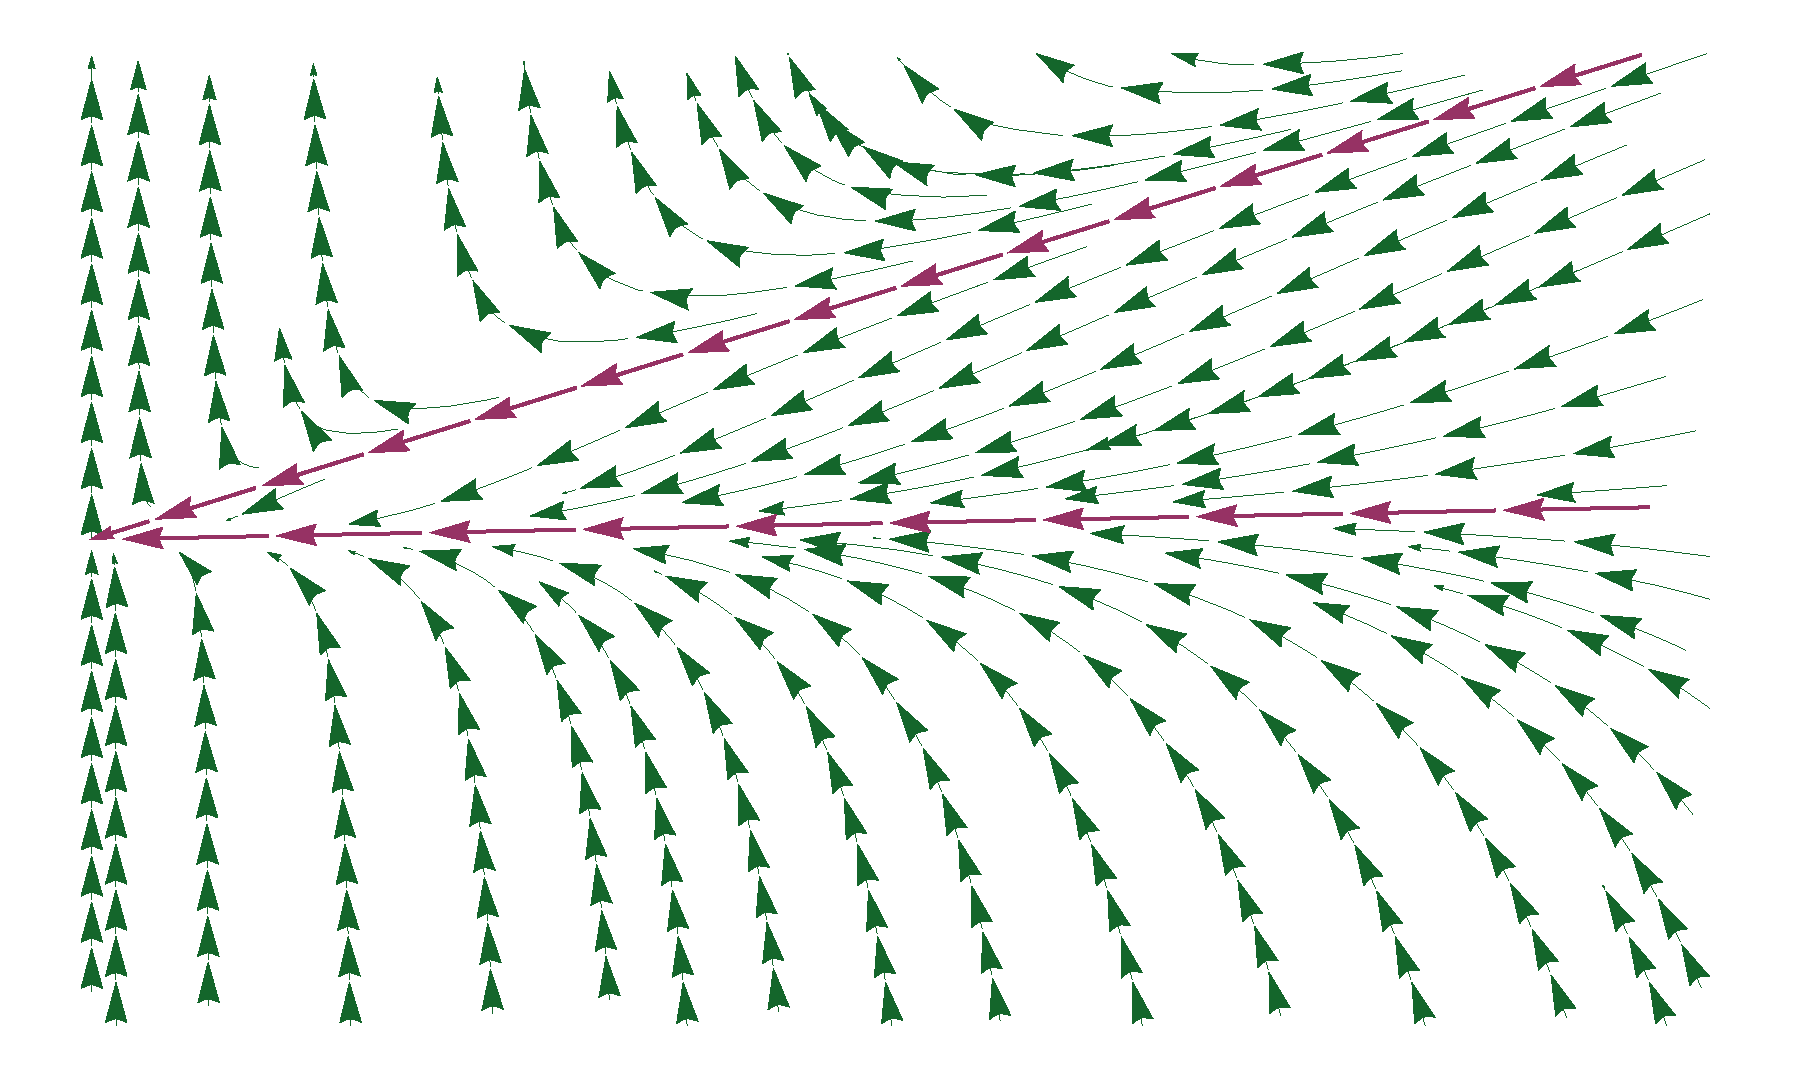
\includegraphics[width=0.9\textwidth]{Cover2.pdf}
        \end{figure}
                
        % 4. Degree Info: Using italics to separate it visually from the names
        {\scshape{Master's Thesis in Physics} \par}
        \vspace{0.1cm}
        
        % 5. Author
        {\slshape\normalsize carried out by \par}
        \vspace{0.1cm}
        {\Large Sophie Lund Wagner \par}
        
        \vspace{0.4cm}
        % 6. Supervisors: Grouped neatly at the bottom
        {\slshape\normalsize under the supervision of \par}
        \vspace{0.1cm}
        {\Large Francesco Sannino \par}
        
        \vspace{0.4cm}
        
        {\slshape\normalsize and co-supervision of \par}
        \vspace{0.1cm}
        {\Large Giacomo Cacciapaglia \par}
        
        %\vspace{1.0cm}
        %{\large May 2026}
        
    \end{center}
\end{titlepage} %<------------ 


\section*{Abstract}

Motivated by the search of possible extensions of the Standard model. We study the conditions for complete asymptotic freedom in a class of chiral gauge theories motivated by grand unified model building and the search for ultraviolet-complete theories. The models are based on the generalised Georgi--Glashow and Bars--Yankielowicz theories with an $\SU(N)$ gauge group. We consider two extensions of these models featuring a scalar field transforming as either a fundamental or an adjoint under the gauge group. In both scenarios, we incorporate multiple chiral fermion families. Using one-loop renormalisation group equations, we systematically analyse the interplay between gauge, Yukawa, and quartic couplings required for all interactions to remain asymptotically free in the ultraviolet. We find that for both representations of scalars, complete asymptotic free models can be found for a specific amount of colours, vector-like families and chiral families. 
\thispagestyle{empty}

\setcounter{tocdepth}{1}

\thispagestyle{empty}
\tableofcontents
\newpage
\section*{Preface and Acknowledgements}

In writing this thesis AI tools were not used to generate text. However, they were utilised in the research progress and for grammatical refinement, alongside the XXX extension on VSCode. Figures were generated using Mathematica, Python and TikZ. Beta functions were generated using the Mathematica package RGBeta \cite{Thomsen:2021ncy}, other packages such as SARAH \cite{Staub:2008uz} and PyR@te \cite{Sartore:2020gou} can also be used for similar purposes. 

The main results of this thesis have been made available as a preprint on arXiv \cite{Cacciapaglia:2026pwh}: Giacomo Cacciapaglia, Francesco Sannino, and Sophie Wagner: \textit{Complete asymptotically free chiral theories}. Chapters \ref{chap:CAF}, \ref{chap:chiralmodels}, \ref{chap:conc}, the abstract, and parts of the appendix is heavily adapted from this preprint. 

I would like to thank\dots
\newpage
\chapter{Introduction}
The most successful model of physics is the Standard Model (SM) of particle physics \cite{Glashow:1961tr, Weinberg:1967tq}. Its description and prediction of elementary particle interactions have been found to be experimentally verified with up to 12 digits of precision \cite{Fan:2022eto}. The predictive power of the SM establishes it as our foundational theory of nature \cite{SLAC-SP-017:1974ind,E598:1974sol,PLUTO:1978jrw, CDF:1995wbb, D0:1995jca,UA1:1983mne, UA1:1983crd, UA2:1983mlz, UA2:1983tsx}. 

Historically, one of the most significant theoretical issues, that the model had to overcome was explaining the generation of mass of force carriers and fermions. A solution to this problem was proposed already in the 1960's by Higgs \cite{Higgs:1964ia, Higgs:1966ev}, which was discovered half a century later \cite{ATLAS:2012yve}, adding to the already successful model. Despite the model's ability to predict physical observables to high accuracy, the model remains an incomplete theory. On the phenomenological side alone, it leaves several fundamental questions unanswered, including: \textit{Why there is a flavour mass hierarchy? Where the matter-antimatter asymmetry comes from? How does Einstein's theory of gravity fit in? And what is dark matter?} 

Furthermore, the model is an effective field theory, meaning the model cannot be valid across all energy scales. This attribute of the model originates from the requirement of having a renormalisable theory as our foundational model. Renormalisation introduces a \textit{running} of the couplings, which greatly affect the Standard Model. The theory of strong interactions (QCD) has a gauge coupling which converges to zero at high energies, however at low energies the coupling diverges, and the famous characteristic of QCD emerges: confinement \cite{Gross:1973id}. This renders perturbative predictions invalid in the IR. In contrast, the electromagnetic interactions (QED) behaves oppositely. Its gauge coupling diverges in the UV leaving us with a incomplete description at high energies. Thus, the Standard Model has neither a free nor an interacting ultraviolet fixed point for all its couplings, leaving us with an effective field theory. 

To address some of these phenomenological questions and extend the SM to higher energies, Grand Unified Theories (GUT)s \cite{Georgi:1974yf, Fritzsch:1974nn, Pati:1974yy, Bai:2021tgl, Langacker:1980js} have been prosed as extensions of the SM. These aim to unify the electromagnetic, weak, and strong force into a single coupling described by a single gauge group. To ensure the validity of these models to energies up to the Planck scale at $10^{19}\,$GeV, where quantum gravitational effects are expected to emerge. The unified gauge coupling in such theories is often \textit{asymptotically free}, while most often the Yukawa and quartic couplings are left untamed in the UV. For gauge-fermion theories without scalars a landscape approach to GUT-model building can be found in \cite{Cacciapaglia:2025nff}.

Theories which are asymptotically free in all couplings, and where the Yukawa and quartic couplings tends to zero at the same rate or faster than the gauge coupling, are known as \textit{complete asymptotically free} (CAF) models \cite{Cheng:1973nv,Gross:1973ju,Holdom_2015,Giudice:2014tma,Pica:2016krb,Callaway:1988ya,Hansen:2017pwe,Zimmermann:1984sx}. These models are valid at arbitrarily high energy, since they have UV fixed points. 

The SM and its extensions are chiral-gauge Yukawa theories, it is therefore paramount to understand UV behaviour of such models. To maintain a general approach, without restricting our focus to one specific model as done in \cite{Giudice:2014tma}, we investigate and construct CAF chiral-gauge Yukawa theories by addressing the following question:

\begin{mdframed}[style=thesisbox]
    \begin{center}
        {\large\textsc{How can we construct chiral-gauge Yukawa theories with different scalar representations such that they remain completely asymptotically free?}}
    \end{center}
\end{mdframed}

In this thesis we will approach this question by considering the generalised Georgi--Glashow (GG)\cite{Georgi:1974sy,Georgi:1974yf} and the Bars--Yankielowicz (BY) \cite{Bars:1981se} models. The IR behaviour of these models in the absences of scalar have been widely investigated in \cite{Appelquist:2000qg,Bolognesi:2020mpe,Csaki:2021xhi,Bolognesi:2021yni,Bolognesi:2021hmg,Bai:2021tgl,Bolognesi:2023xxv,Li:2025tvu,Li:2026ayh}. In this thesis, we will instead consider the high energy behaviour as in \cite{Molgaard:2016bqf}, but extending this work by including a scalar in the adjoint representation. 

We systematically evaluate the impact of adding a single scalar in the fundamental representation and the adjoint representation separately. These two representations of scalars are vital to GUTs. The fundamental scalar plays the role of the Higgs in the SM, breaking the electroweak symmetry and generating massive force carriers and fermions. The adjoint scalar allows us to, at low energies, realise the SM, effectively breaking the gauge group (or a subgroup) of the GUT down to the gauge sector of the SM \cite{Georgi:1974yf, Li:1973mq}. To make the analysis more general, we also consider the changing the number of Chiral families, and the effects of this on the CAF regions. 

This thesis is organised as follows. In Chapter \ref{chap:RG}, we introduce the renormalisation group, and through this beta functions and asymptotic freedom, to lay the ground work of the CAF framework used in this project. In Chapter \ref{chap:GUT}, we further our understanding of the SM, its shortcomings and through this the motivation of GUTs. We will also investigate the $\SU(5)$ GUT to understand the dynamics and principles of GUTs. With this knowledge we can then understand the approach to finding CAF theories described in Chapter \ref{chap:CAF}. Equipped with the CAF framework, we introduce the general Chiral models in Chapter \ref{chap:chiralmodels} and systematically investigate possible CAF regions of the theory. We first consider the models without a scalar in Section \ref{sec:noscalar}, then adding one fundamental scalar in Section \ref{sec:fundscalar}, and finally considering the adjoint scalar in Section \ref{sec:adj}. This analysis leads us to the answer of our question, which is given in Chapter \ref{chap:conc} and includes a summary table stating CAF viability of all considered models.



\chapter{The Renormalisation Group}
\label{chap:RG}
In this chapter we will first study the renormalisation group equations to understand how the couplings change with energy. This is achieved by first introducing the Callan-Symanzik equation \cite{Callan:1970yg, Symanzik:1970rt, Symanzik:1971vw}, followed by the computation of the non-Abelian gauge beta function. From this we will consider different scenarios of the coupling's behaviour when the energy scale is changed. Through this we introduce a core concept of the thesis: \textit{asymptotic freedom}.

\section{Renormalisation}
Quantum Field Theory (QFT) gives us the tools we need to understand the Universe's smallest structures. However, when applying this framework one encounters divergences when computing physical quantities. This raises a fundamental question: \textit{at what scale is the theory valid?} One framework to address this question is the renormalisation group (RG) \cite{Gell-Mann:1954yli}, particularly through \textit{Wilson}'s approach \cite{Wilson:1983xri, Wilson:1974mb}. The formalism provides a physical understanding of one of the key features of QFT, namely, renormalisation \cite{Pernow:2021fvb}.

These divergences arise when computing loop amplitudes, which must yield finite values to correspond to physical observables. The divergences are specifically encountered when integrating over internal momenta when computing Feynman diagrams \cite{Pernow:2021fvb}. To obtain finite amplitudes, one needs to first regularise the divergences. Methods of this include cutoff \cite{Peskin:1995ev}, Pauli-Villars \cite{Pauli:1949zm}, and dimensional regularisation \cite{tHooft:1972tcz}. All of these introduce an energy scale dependence, which we will call $\Lambda$, into the theory. We will see an example of this later in Section \ref{sec:betafunc}. 

The scale dependence introduced through the regularisation is not only a mathematical feature of the approach, but a physical attribute of the model. In Wilson's interpretation, the cutoff $\Lambda$ represents the energy scale at which the effective theory breaks down. The main effect of this approach is that masses and the coupling constants evolve as a function of $\Lambda$. An objective of this approach is therefore to extract how the coupling constants evolve with the energy scale. 

A theory will generally be described by a set of parameters $\{g_i\}$. These are mass parameters and couplings. If we wish to examine different length scales\footnote{Recall that using natural units where $c=\hbar=1$ the de Broglie wavelength is $p\propto1/\lambda$. In the relativistic limit this means that energy scales as one over length. So high energies is equal to short distances and vice versa. }, we can introduce a parameter $h$ to understand how the masses and couplings change with the energy scale at which we probe our theory
\begin{align} 
    g_i(\Lambda)\to g_i(\Lambda/h)\,,
\end{align}
where $h>1$ allows us to consider larger length scales, this is called \textit{coarse-graining} \cite{Lancaster:2014}. The variation of the parameter $h$ ensures rescaling of the cutoff $\Lambda$, and will therefore affect the values of the couplings. 

For a system with two couplings $g_i$ with $i=1,2$, the scale dependence can be visualised by multiple trajectories which change as the energy scale changes. These trajectories are called a renormalisation group trajectory and collection of these depict the renormalisation group flow \cite{Lancaster:2014}. An illustrated example can be found in Figure~\ref{fig:RGflow}. 
\begin{figure}[htbp]
    \centering
        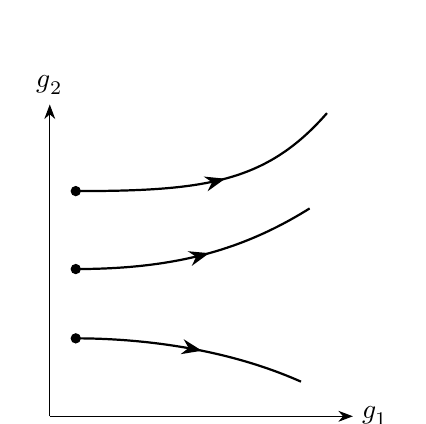
\begin{tikzpicture}[
            scale=1.1,
            >={Stealth[scale=1.1]},
            flow/.style={
                thick,
                postaction={decorate}, 
                decoration={markings, mark=at position 0.55 with {\arrow{>}}}
            }
        ]

            % Axes
            \draw[->] (0,0) -- (3.5,0) node[right] {$g_1$};
            \draw[->] (0,0) -- (0,3.6) node[above] {$g_2$};

            % Top curve (Starts a bit further back, stays flat longer, curves up sharply)
            \filldraw (0.3, 2.6) circle (1.5pt);
            \draw[flow] (0.3, 2.6) .. controls (1.8, 2.6) and (2.5, 2.7) .. (3.2, 3.5);

            % Middle curve (Starts further forward, curves up gently and earlier)
            \filldraw (0.3, 1.7) circle (1.5pt);
            \draw[flow] (0.3, 1.7) .. controls (1.4, 1.7) and (2.2, 1.9) .. (3.0, 2.4);

            % Bottom curve (Starts in between, stays flat then drops off at the end)
            \filldraw (0.3, 0.9) circle (1.5pt);
            \draw[flow] (0.3, 0.9) .. controls (1, 0.9) and (2, 0.8) .. (2.9, 0.4);

        \end{tikzpicture}
        \vspace{0.5cm} % Alignment spacing
        \caption{Illustrative RG trajectories in the $(g_1,g_2)$ parameter space. The black dots mark the initial coupling values, with the arrows showing the RG flow, which point towards the UV.} 
        \label{fig:RGflow}
\end{figure}
% We can also consider the change of the coupling as In this space, \textit{fixed points} can occur. These are points in the multidimensional space defined by the set of couplings, which does not change with coarse-graining. \comment{insert sketch}

Now having reviewed the Wilsonian framework, we will follow the standard QFT approach of renormalising the Lagrangian. It is crucial here to distinguish the Wilsonian approach from the Callan--Symanzik approach (which we follow from now and in the following section). In Wilson's framework, the cutoff $\Lambda$ is a physical scale, and the RG flow describes how the effective theory changes as we integrate out physical high-energy modes. In contrast, the standard QFT approach aims to remove the cutoff entirely by taking the limit $\Lambda\to\infty$. To keep physical quantities finite, we absorb the divergences into counterterms, a process which inherently introduces a new, arbitrary energy scale called the renormalisation scale, $\mu$. Unlike Wilson's $\Lambda$, $\mu$ is strictly a mathematical artefact. Therefore in this approach, physical observables, such as the S-matrix, remain invariant under the change of the arbitrary energy scale $\mu$. 

We do this through renormalisation of the theory. Renormalisation ensures that the parameters of the Lagrangian change with the energy scale, effectively countering the effect of regularisation. Thus, the Lagrangian can be expressed as
\begin{equation}
    \mathcal{L}_{\mathrm{0}}= \mathcal{L}_{\mathrm{Renorm}}+ \mathcal{L}_{\mathrm{ct}}\label{eq:Barelag}
\end{equation} 
where $ \mathcal{L}_{\mathrm{0}}$ is the so-called \textit{bare} Lagrangian, which represent the theory's original Lagrangian containing the bare parameters which are the non-renormalised parameters. On the RHS $\mathcal{L}_{\mathrm{Renorm}}$ describes the renormalised Lagrangian, whose parameters are physical and depend on the energy scale,  and $ \mathcal{L}_{\mathrm{ct}}$ describes the necessary counterterms, which absorb the divergences. In this approach, we have already sent our cutoff to infinity, so how do we extract the RG flows of the parameters? We can use that the renormalisation of the Lagrangian depends on conditions at some renormalisation scale \cite{Peskin:1995ev}. Let us consider an example: a non-Abelian theory consisting of massless fermions. This theory has the bare Lagrangian
\begin{align}
    \mathcal{L}_0 = -\frac{1}{4} F^{a}_{0\mu\nu} F_0^{a\,\mu\nu}
+ \bar{\psi}_0 i \gamma^\mu D_\mu \psi_0\,,\label{eq:LagnonAbelian}
\end{align} 
with
\begin{equation}
D_\mu = \partial_\mu + i g_0 A^a_{0\mu} t^a\,, \qquad F^a_{\mu\nu}=\partial_\mu A_\nu^a-\partial_\nu A^a_\mu+g_0 f^{abc}A_\mu^bA_\nu^c\,,
\end{equation}
where \(g_0\) denotes the bare coupling constant, $\gamma^\mu$ are the Dirac matrices which obey the Clifford algebra, $f^{abc}$ is the structure constant of the concerned gauge group, and the gauge indices of the fermions have been suppressed for clarity. The bare parameters are related to the renormalised parameters as
\begin{equation}
\psi_0 = \sqrt{Z_2}\,\psi, \qquad
A^a_{0\mu} = \sqrt{Z_3}\,A^a_\mu, \qquad
g_0 = \mu^\epsilon Z_g\, g\,, \label{eq:Renormvalue}
\end{equation}
where $\mu^\epsilon$ is added to ensure a dimensionless coupling when using the dimensional regularisation scheme, which will be further explained in the subsequent section.
 
Now that we understand the motivation of the RG, we can use our knowledge to write down and equation which describes how the physical parameters of the theory will change with the energy scale, this is the \textit{Callan-Symanzik equation} \cite{Callan:1970yg,Symanzik:1970rt,Symanzik:1971vw}. 

\section{The Callan-Symanzik Equation}
In the process of dimensional regularisation the energy scale $\mu$ is introduced. This energy scale is not fixed and could just as well be given by $\mu'$. The only thing that needs to remain fixed is the bare Lagrangian $\mathcal{L}_{
\mathrm{0}}$ (see Eq.~\eqref{eq:Barelag}). 
Recall that the fields rescale as $\phi_0 = \sqrt{Z}\,\phi$ (see Eq.~\eqref{eq:Renormvalue}). This can be generalised for $n$ fields, so we can write the renormalised Green's function as a scaling of the bare Green's function
\begin{align}
    \langle \Omega | T\phi(x_1)\phi(x_2)\cdots\phi(x_n) |\Omega \rangle = Z^{-n/2} \langle \Omega | T\phi_0(x_1)\phi_0(x_2)\cdots\phi_0(x_n) |\Omega \rangle\,.
\end{align}
The bare Lagrangian will, by definition, remain scale invariant, since it is describing the underlying theory. Scale-dependency emerges in the renormalised Lagrangian, because it is introduced to remove the cutoff-dependent $\lambda_0$ with a running coupling $\lambda$. As already pointed out, this scale could be chosen as $\mu'$ by mapping $\lambda\to\lambda'$ and $Z\to Z'$ \cite{Peskin:1995ev}. We can perform this shift $\delta\mu$ explicitly, which results in
\begin{align}
    \mu\to \mu+\delta \mu\,,\\\lambda\to\lambda+\delta\lambda\,,\\Z\to Z+\delta Z\,.
\end{align}
The shift of the Green's function is thus only dependent on the shift of the renormalisation constant $Z$
\begin{align}
    G^{(n)}\to G^{(n)}+\delta G^{(n)} = \left(Z^{-n/2}+\delta\left(Z^{-n/2}\right)\right) G_0^{(n)}\,,
\end{align}
where $G^{(n)}(x_1,\dots,x_n)=\langle \Omega | T\phi(x_1)\phi(x_2)\cdots\phi(x_n) |\Omega \rangle $. We can expand the second term
\begin{align}
    \left(\delta\left(Z^{-n/2}\right)\right)= \frac{ \partial \left(Z^{-n/2}\right)}{\partial Z}\delta Z=-\frac{n}{2} Z^{-n/2}\frac{\delta Z}{Z}= n \delta \eta\,, \label{eq:defeta}
\end{align}  
where $\delta\eta:=-\frac{1}{2}\frac{\delta Z}{Z}$. Thus, the shift in a renormalised Green's function is a field scaling 
\begin{align}
    G^{(n)}\to (1+n\delta\eta ) G^{(n)}\,.
\end{align}
We can now use the fact that the $n$-point Green's function $G^{(n)}$ is not only a function of spacetime but also the renormalisation scale and the renormalised coupling. $G^{(n)}(x_1,\dots,x_n;\mu,\lambda)$. Thus, the shift can be rewritten as
\begin{align}
    \delta G^{(n)} = \frac{\partial G^{(n)}}{\partial \mu} \delta \mu + \frac{\partial G^{(n)}}{\partial \lambda} \delta \lambda\,.
\end{align}
We can use the definition from Eq.~\eqref{eq:defeta} to obtain 
\begin{align}
     \left[\frac{\partial}{\partial \mu} \delta \mu + \frac{\partial}{\partial \lambda} \delta \lambda- n\delta\eta \right]G^{(n)}(x_1,\dots,x_n;\mu,\lambda)=0\,,\label{eq:CSeq1}
\end{align}
and by defining 
\begin{align}
    \beta\equiv \frac{\mu}{\delta\mu}\delta\lambda\,, \qquad  \gamma\equiv- \frac{\mu}{\delta\mu}\delta\eta\,,\label{eq:beta0}
\end{align}
the expression in Eq.~\eqref{eq:CSeq1} can be rewritten as 
\begin{align}
     \left[\mu\frac{\partial}{\partial \mu}  + \beta \frac{\partial}{\partial \lambda} + n\gamma \right]G^{(n)}(x_1,\dots,x_n;\mu,\lambda)=0\,.
\end{align}
It is of importance to understand what the parameters $\beta$ and $\gamma$ depend on. First, they cannot depend on $n$ since the expression holds for all $n-point$ functions. Furthermore, they are independent of $x_i$, since the parameters are properties of the theory itself and not kinematic effects. Because the Green's function is renormalised, they cannot depend on the cutoff $\Lambda$. Additionally, the parameters cannot depend explicitly on the energy scale; this can be seen by the fact that both parameters are dimensionless, and the energy scale is not. The only dependency of the parameters are thus the couplings, so we can write 
\begin{align}
     \left[\mu\frac{\partial}{\partial \mu}  + \beta(\lambda) \frac{\partial}{\partial \lambda} + n\gamma(\lambda) \right]G^{(n)}(\{x_i\};\mu,\lambda)=0\,.
\end{align}
This is the Callan--Symanzik equation, which describes how the change of the scale at which we are probing our theory is balanced by changes to the two parameters $\beta$ and $\gamma$. The case above is only for a theory with one massless field and one coupling. An additional coupling translates to an additional $\beta$ parameter, and an additional field ensures that there will be an extra $\gamma$ parameter. Furthermore, it should be noted that this analysis changes when considering a massive theory. Since the mass is also renormalised, the Green's function will also depend on the mass, which runs with the energy scale $\mu$. The general Callan--Symanzik equation is then expressed as \cite{Srednicki2007}
\begin{align}
     \left[\mu\frac{\partial}{\partial \mu}  + \beta(\lambda) \frac{\partial}{\partial \lambda} +\gamma_m\frac{\partial }{\partial \ln m}+ n\gamma(\lambda) \right]G^{(n)}(\{x_i\};\mu,\lambda, m)=0\,,
\end{align}
where $\gamma_m=\frac{\partial \ln m}{\partial \ln \mu}$ is called the \textit{anomalous dimension of the mass} and describes how changing the energy scale affects the renormalised mass \cite{Srednicki2007}. 

With the RG framework established, we shift our focus to the introduced parameter $\beta$. The subsequent section provides a deeper insight into the mechanics of the beta function by considering an example. Through this example we will apply the mathematical tools we have already discussed: first regularisation and then renormalisation. This approach also allows us to understand how the couplings can run.

\section{The beta function} \label{sec:betafunc}
To better understand the new parameters $\beta$ and $\gamma$, we can consider the limit in which $\delta\to\partial$ of Eq.~\eqref{eq:beta0}, from which we obtain
\begin{align}
    \beta\equiv \mu\frac{\partial \lambda}{\partial\mu}\,, \qquad  \gamma\equiv- \mu\frac{\partial\eta}{\partial\mu}=-\frac{\mu}{Z}\frac{\partial Z}{\partial \mu}\,.\label{eq:betafunc}
\end{align}
The parameters are referred to as the \textit{beta function} and \textit{anomalous dimension} \cite{Pernow:2021fvb}. As seen from the formula and explained above, the equation shows the coupling's and the field's reaction to the change of the energy scale, respectively. Our interest lies predominantly in the beta function, because this describes the change of the interaction strength between our fields as the energy scale at which we probe our theory changes. The approach to calculating these Callan--Symanzik functions is through the counterterms originating from the renormalisation. We can relate the beta function directly to these.

\subsection{An example: Non-Abelian Lagrangian}
Let us take the example of the bare Lagrangian $\mathcal{L}_\mathrm{0}$ in Eq.~\eqref{eq:LagnonAbelian} describing non-Abelian gauge theories with massless fermions. To generalise the beta function we will extend the theory to include massive fermionic fields effectively adding a term to the bare Lagrangian, so that the full Lagrangian yields \cite{Peskin:1995ev}
\begin{align}
     \mathcal{L}_\mathrm{0} &= \bar{\psi}(i \slashed{\partial} - m)\psi - \frac{1}{4}(\partial_\mu A_\nu^a - \partial_\nu A_\mu^a)^2 + g_0 A_\mu^a \bar{\psi} \gamma^\mu t^a \psi\nonumber \\&\quad- g_0 f^{abc} (\partial_\mu A_\nu^a) A^{\mu b} A^{\nu c} - \frac{1}{4} g_0^2 (f^{eab} A_\mu^a A_\nu^b)(f^{ecd} A^{\mu c} A^{\nu d})\,.\label{eq:LnonA}
\end{align}
In the Lagrangian the third term is the vertex, which we can write in its renormalised form as
\begin{equation}
    \Gamma_{\bar{\psi} A \psi, r}^{(3)} = \Gamma_{\bar{\psi} A \psi}^{(3)} / Z_1 \,.
\end{equation}
Thus, we can express the renormalised coupling using Eq.~\eqref{eq:Renormvalue} as 
\begin{align}
    Z_1 g_r =\mu^{-\epsilon} \sqrt{Z_2} \sqrt{Z_3} \sqrt{Z_2} g_0 = \mu^{-\epsilon} Z_2 Z_3^{1/2} g_0 \implies g_r = \mu^{-\epsilon}\frac{Z_2 Z_3^{1/2}}{Z_1} g_0 \,,
\end{align}
where $g_r$ is the fermion-gauge coupling. We can then consider the beta function (see Eq.~\eqref{eq:betafunc}) of the coupling
\begin{equation}
    \beta(g_r) = \mu \frac{\dd g_r}{\dd\mu}\,.
\end{equation}
From now on, we will drop the subscript on the coupling and set $g_r = g$. We have
\begin{align}
    \beta(g)  &= \mu \frac{\partial}{\partial\mu} \left(\mu^{-\epsilon} \frac{Z_2 Z_3^{1/2}}{Z_1} g_0 \right)\nonumber \\
    &=-\epsilon g +g_0 \left( \frac{Z_2 Z_3^{1/2}}{Z_1} \mu \frac{\partial}{\partial\mu} \ln\left( \frac{Z_2 Z_3^{1/2}}{Z_1} \right) \right) \nonumber\\
    &= -\epsilon g+g \left( \mu \frac{1}{Z_2} \frac{\partial Z_2}{\partial\mu} + \frac{\mu}{2 Z_3} \frac{\partial Z_3}{\partial\mu} - \frac{\mu}{Z_1} \frac{\partial Z_1}{\partial\mu} \right)\,,
\end{align}
where we used that the derivative of the bare coupling is zero $\frac{\partial}{\partial\mu} g_0 = 0$, since the bare parameters, by definition, do not change with the energy scale. 

We can now use the definition of the anomalous dimensions in Eq.~\eqref{eq:betafunc} to identify
\begin{equation}
    \gamma_i = - \frac{\mu}{Z_1}  \frac{\partial Z_i}{\partial\mu} \sim -\mu  \frac{\partial \delta_i}{\partial \mu}\,,
\end{equation}
where we use that $Z_i=1+\delta_i$ where $1$ is the three level contribution and $\delta_i$ the counterterm, and $\delta_i\ll 1$. This allows us to approximate the beta function as
\begin{align}
    \beta(g) =-\epsilon g+ g  \frac{\partial}{\partial\mu} \left( \gamma_1 - \gamma_2 - \frac{1}{2} \gamma_3 \right) \sim-\epsilon g+ g \mu \frac{\partial}{\partial\mu} \left( -\delta_1 + \delta_2 + \frac{1}{2} \delta_3 \right) \,.
\end{align}
Thus, the process of calculating a beta function boils down to computing counterterms and thereby Feynman loop diagrams. In general, we distinguish between the loop order of the beta function. Let us compute the example we have been considering so far: the one-loop gauge beta function of the non-Abelian theory with one massive fermionic field. 

We will only do one of the calculations here explicitly, as this provides a clear example of how to perform such calculations. The different contributions come from the one-loop diagrams of  the fermion-gauge boson vertex
\begin{align}\delta_1\sim \raisebox{-0.8cm}{\feynmandiagram [vertical=a to b, small] {
        a -- [photon] b ,
        f1 -- [fermion] c -- [fermion] b -- [anti fermion] d -- [fermion] f2,
        c -- [photon] d,
    };}+\raisebox{-0.8cm}{\feynmandiagram [vertical=a to b, small] {
        a -- [photon] b ,
        f1 -- [fermion] c -- [photon] b -- [photon] d -- [fermion] f2,
        c -- [fermion] d,
    };}\,,\label{eq:delta1}
\end{align}
the fermion self-energy
\begin{align}
    % Electron Self-Energy
    \delta_2 &\sim \raisebox{-0.1cm}{
        \begin{tikzpicture}
            \begin{feynman}
                \vertex (a);
                \vertex [right=1cm of a] (c);
                \vertex [right=1.5cm of c] (d);
                \vertex [right=1cm of d] (b);
                \diagram* {
                    (a) -- [plain] (c) -- [fermion] (d) -- [plain] (b),
                    (c) -- [photon, half left, looseness=1.5] (d),
                };
            \end{feynman}
        \end{tikzpicture}
    } \,,\label{eq:delta2}
\end{align}
and the gauge boson self-energy 
\begin{align}
    % Vacuum Polarisation (Fermion Loop)
    \delta_3 \sim \raisebox{-0.6cm}{
        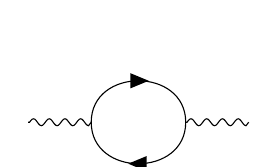
\begin{tikzpicture}
            \begin{feynman}
                \vertex (a);
                \vertex [right=0.8cm of a] (c);
                \vertex [right=1.2cm of c] (d);
                \vertex [right=0.8cm of d] (b);
                \diagram* {
                    (a) -- [photon] (c),
                    (c) -- [fermion, half left, looseness=1.5] (d) -- [fermion, half left, looseness=1.5] (c),
                    (d) -- [photon] (b),
                };
            \end{feynman}
        \end{tikzpicture}
    } + \raisebox{-0.6cm}{
        % Boson/Gauge Loop
        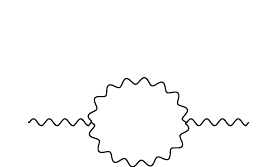
\begin{tikzpicture}
            \begin{feynman}
                \vertex (a);
                \vertex [right=0.8cm of a] (c);
                \vertex [right=1.2cm of c] (d);
                \vertex [right=0.8cm of d] (b);
                \diagram* {
                    (a) -- [photon] (c),
                    (c) -- [photon, half left, looseness=1.5] (d) -- [photon, half left, looseness=1.5] (c),
                    (d) -- [photon] (b),
                };
            \end{feynman}
        \end{tikzpicture}
    }  + \raisebox{-0.6cm}{
        % Scalar Loop
        \begin{tikzpicture}
            \begin{feynman}
                \vertex (a);
                \vertex [right=0.8cm of a] (c);
                \vertex [right=1.2cm of c] (d);
                \vertex [right=0.8cm of d] (b);
                \diagram* {
                    (a) -- [photon] (c),
                    (c) -- [scalar, half left, looseness=1.5] (d) -- [scalar, half left, looseness=1.5] (c),
                    (d) -- [photon] (b),
                };
            \end{feynman}
        \end{tikzpicture}
    } + \raisebox{-0.3cm}{ 
        % Adjusted raisebox because legs are lower now
        
\begin{tikzpicture}
            \begin{feynman}
                % Angled legs: start below the interaction vertex
                \vertex (a) at (0, -0.3); 
                \vertex (c) [dot] at (1.0, 0); % The centre
                \vertex (b) at (2.0, -0.3);
                % The loop anchor
                \vertex (d) at (1.0, 0.8); 
                \diagram* {
                    (a) -- [photon] (c) -- [photon] (b),
                    (c) -- [photon, half left, looseness=1.6] (d) -- [photon, half left, looseness=1.6] (c),
                };
            \end{feynman}
        \end{tikzpicture}
    }\,.\label{eq:delta3}
\end{align}
The diagrams in Eq.~\eqref{eq:delta1} represent the vertex renormalisation. The first diagram is also present in the vertex corrections of Abelian theories. The second diagram is specific to non-Abelian theories, since it includes self-interactions between the gauge bosons. Thus, $\delta_1$ will absorb the divergences of these two one-loop diagrams. In Eq.~\eqref{eq:delta2} $\delta_2$ is defined to renormalise the fermion wave function. Lastly, Eq.~\eqref{eq:delta3} represents the gauge boson wave function corrections, coming from four one-loop diagrams, including a fermion loop, a ghost loop,\footnote{Faddeev--Popov ghosts are unphysical fields and are introduced to combat gauge redundancy \cite{Peskin:1995ev}.} and two including gauge boson self-interactions. The last diagram is generally called a tadpole diagram.\footnote{This diagram can equal zero depending on the chosen regularisation scheme \cite{Peskin:1995ev}.}

We choose to focus on the contributions from the fermion self-energy, $\delta_2$ in Eq.~\eqref{eq:delta2}. The other terms are given by \cite{Peskin:1995ev}
\begin{align}
   \delta_1 &= -\frac{g^2}{(4\pi)^{d/2}} \frac{\Gamma(2 - d/2)}{(\mu^2)^{2-d/2}} [C_2(R) + C_2(G)] \,,\label{eq:delta1expr}\\
   \delta_3& =\frac{g^2}{(4\pi)^{d/2}} \frac{\Gamma(2 - d/2)}{(\mu^2)^{2-d/2}} \left[ \frac{5}{3} C_2(G) - \frac{4}{3} n_f T(R) \right]\,,\label{eq:delta3expr} 
\end{align}
where $n_f$ is the number of different fermion fields. There are three group-theoretical (see Appendix \ref{app:GT}) constants in the equations, two of them depend on the gauge group and the representation $R$ of the fermionic field(s): $T(R)$ is the Dynkin index and $C_2(R)$ is the quadratic Casimir index. The factor $C_2(G)$ is the quadratic Casimir as well, but of the gauge group $G$ (see Appendix~\ref{app:Lie}).

To compute the renormalised fermion's self-energy \(-i \Sigma_R(p^2)\), we need to include the counterterm contributions. These terms absorb the UV divergences of the loop diagrams, rendering the physical quantity finite through a proper choice of  $\delta_2$ and $\delta_m$. Thus, we need to calculate the sum of the two diagrams, the loop diagram and the corresponding counterterm, given by 
\begin{align}
     -i \Sigma_{\mathrm{R}}(p^2)=-i \Sigma_{\text{1 loop}}(p^2)+i(\slashed{p}\delta_2-\delta_m)= \raisebox{-0.1cm}{
        \begin{tikzpicture}
            \begin{feynman}
                \vertex (a);
                \vertex [right=1cm of a] (c);
                \vertex [right=1.5cm of c] (d);
                \vertex [right=1cm of d] (b);
                \diagram* {
                    (a) -- [plain] (c) -- [fermion] (d) -- [plain] (b),
                    (c) -- [photon, half left, looseness=1.5] (d),
                };
            \end{feynman}
        \end{tikzpicture}
    } 
    + 
    \raisebox{-0.1cm}{
        \begin{tikzpicture}
            \begin{feynman}
                \vertex (a) at (0, 0); 
                \node [draw, circle, minimum size=10pt, inner sep=0pt] (c) at (1.2, 0) {};
                \vertex (b) at (2.4, 0);
                % Draw the cross manually
                \draw (c.north west) -- (c.south east);
                \draw (c.north east) -- (c.south west);
                \diagram* {
                    (a) -- [plain] (c) -- [plain] (b),
                };
            \end{feynman}
        \end{tikzpicture}
    }\,,\label{eq:fermselfenergy}
\end{align}
where the structure of the counterterm originates for the kinetic term of fermion in the Lagrangian in Eq.~\eqref{eq:LnonA}. To compute the one-loop diagram, we need the three following Feynman rules \cite{Peskin:1995ev}:
\begin{align}
  &\text{Vertex: } ig \gamma^\mu t^a\label{eq:fey1}\,,\\
  &\text{fermion propagator: } \frac{i(\slashed{p} + m)}{p^2 - m^2 + i \epsilon}\,, \\
  &\text{boson propagator:} -\frac{i g_{\mu\nu}}{q^2 + i \epsilon}\label{eq:fey3}\,,
\end{align}
where the boson propagator is found using the Feynman-'t Hooft gauge.


The diagram has an incoming fermion momentum \(p\), an internal fermion momentum \(k\), and an internal boson momentum \(p-k\). We can use this together with the Feynman rules (Eqs. \eqref{eq:fey1}-\eqref{eq:fey3}) to write
\begin{align}
  -i \Sigma_{\text{1 loop}}(p^2) &=\raisebox{-0.7cm}{
    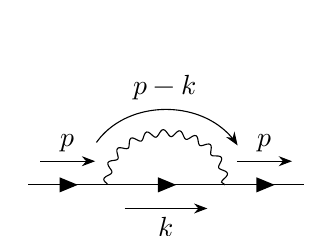
\begin{tikzpicture}
        \begin{feynman}
            \vertex (a);
            \vertex [right=1cm of a] (c);
            \vertex [right=1.5cm of c] (d);
            \vertex [right=1cm of d] (b);
            \diagram* {
                (a) -- [fermion, momentum=\(p\)] (c) -- [fermion, momentum'=\(k\)] (d) -- [fermion, momentum=\(p\)] (b),
                (c) -- [photon, half left, looseness=1.5, momentum=\(p-k\)] (d),
            };
        \end{feynman}
    \end{tikzpicture}
}\nonumber\\&= \int \frac{\dd^4 k}{(2\pi)^4} ig \gamma^\mu t^a \frac{i(\slashed{k} + m)}{k^2 - m^2 + i \epsilon} ig \gamma^\nu t^a \frac{-i g_{\mu\nu}}{(p-k)^2 + i \epsilon}\nonumber\\
  &= -g^2\int \frac{\dd^4 k}{(2\pi)^4} \gamma^\mu t^a \frac{\slashed{k} + m}{k^2 - m^2 + i \epsilon} \gamma_\mu t^a \frac{1}{(p-k)^2 + i \epsilon}\,.
\end{align}
We can now use the group theory relation of the operators \(t^a t^a = C_2(R) \mathbb{1}\) (see Appendix \ref{app:Lie}) to simplify the expression, such that we obtain
\begin{align}
  -i \Sigma_{\text{1 loop}}(p^2)&= -g^2 C_2(R) \int \frac{\dd^4 k}{(2\pi)^4} \gamma^\mu \frac{\slashed{k} + m}{k^2 - m^2 + i \epsilon} \gamma_\mu \frac{1}{(p-k)^2 + i \epsilon}\,.
\end{align}
To simplify the numerator we use the relations $\gamma^\mu\gamma_\mu=d\mathbb{1}$ and $\gamma^\mu\gamma_\mu\gamma^\nu=(2-d)\gamma^\nu$ \cite{Peskin:1995ev}, which yields
\begin{align}
   \gamma^\mu(\slashed{k}+m)\gamma_\mu&=\gamma^\mu\gamma^\nu k_\nu\gamma_\mu+\gamma^\mu m\gamma_\mu=k_\nu\gamma^\mu\gamma^\nu\gamma_\mu+md\mathbb{1}=k_\nu(2-d)\gamma^\nu+md=-((d-2)\slashed{k} - md)\,.
\end{align}
This results in the following integral
\begin{align}
  -i \Sigma_{\text{1 loop}}(p^2) = g^2 C_2(R) \int \frac{\dd^4 k}{(2\pi)^4} \frac{(d-2)\slashed{k} - md}{(k^2 - m^2 + i\epsilon)((p-k)^2 + i\epsilon)} \,.\label{eq:den}
\end{align}
The next step is to use Feynman parameterisation. Utilising this method we can transform the two factors in the denominator in Eq.~\eqref{eq:den} into a single quadratic polynomial in $k$. This polynomial will be squared. Then we can shift the integration momentum $k$ to complete the square leaving us with a spherically symmetric denominator. The price to pay for this is an additional integral over a Feynman parameter. We can write this as
\begin{align}
    \frac{1}{AB} = \int_0^1 \frac{\dd x}{[(1-x)A + xB]^2}\,.\label{eq:Feypar}
\end{align}
To use this method, we first define $A$ and $B$ by considering the denominator in Eq.~\eqref{eq:den}. Then we can expand the expression of the denominator, which yields
\begin{align}
    A &= k^2 - m^2 + i\epsilon \,,\\
    B &= (p-k)^2 + i\epsilon = p^2 + k^2 - 2pk + i\epsilon \,,\\
    D &= (1-x)(k^2 - m^2 + i\epsilon) + x(p^2 + k^2 - 2pk + i\epsilon)\nonumber\\
    &= k^2 - (1-x)m^2 + i\epsilon - i\epsilon x - k^2 x + xp^2 + x k^2 - 2pkx + i\epsilon x \nonumber\\
    &= k^2 + xp^2 - 2pkx - (1-x)m^2 + i\epsilon\,.
\end{align}
We can then complete the square by adding and subtracting $x^2p^2$, allowing us to obtain
\begin{align}
    D&= (k - xp)^2 - x^2p^2 + xp^2 - (1-x)m^2 + i\epsilon \nonumber\\
    &= \ell^2 + x(1-x)p^2 - (1-x)m^2 + i\epsilon \nonumber\\
    &= \ell^2 - \Delta + i\epsilon\,,\label{eq:denny}
\end{align}
with $\Delta = -x(1-x)p^2 + (1-x)m^2$ and $ \ell = k - xp$. Next, the numerator in Eq.~\eqref{eq:den} is rewritten in terms of the new variables, from which we obtain
\begin{align}
    N &= (d-2)\slashed{k} - dm \implies N=(d-2)(\slashed{\ell} + x\slashed{p}) - dm\,.\label{eq:numny}
\end{align}
We can now insert the redefinition of the numerator (Eq.~\eqref{eq:numny}) and the denominator (Eq.~\eqref{eq:denny}) using the Feynman parametrisation (Eq.~\eqref{eq:Feypar}) on our integral in Eq.~\eqref{eq:den}. Then we perform a Wick rotation to perform a spherical integral in four-dimensions. We do this by rotating the temporal component of the momentum four-vector $\ell_E = -i \ell^0$. This effectively transforms Minkowski space into a four-dimensional Euclidean space. This changes our momentum related terms to: 
\begin{align}
    &\dd^4\ell = \dd\ell_0 d^3\vec{\ell} \implies i \dd\ell_E^0 \dd^3\vec{\ell}_E = i \dd^4\ell_E\,,\\
    &\ell^2 - \Delta \implies -\ell_E^2 - \Delta = -(\ell_E^2 + \Delta) \,,
\end{align}
where we have dropped the $i\epsilon$ term, since in Euclidean space the denominator no longer vanishes for on shell particles. This leaves us with the Wick rotated integral
\begin{align}
    -i \Sigma_{\text{1 loop}}(p^2)= g^2 C_2 \int_0^1 \dd x \int \frac{\dd^4(i\ell_E)}{(2\pi)^4} \frac{(d-2)(x\slashed{p}) - dm}{[\ell_E^2 + \Delta]^2}\,,\label{eq:nyint}
\end{align}
where the terms linear in $\slashed{\ell}$ vanish since it is an odd function evaluated over a symmetric interval. To solve the integral, we can use the general relation \cite{Peskin:1995ev} given by
\begin{align}
    \int \frac{\dd^d \ell_E}{(2\pi)^d} \frac{1}{[\ell_E^2 + \Delta]^n} &= \Delta^{-n} \left(\frac{\Delta}{4\pi}\right)^{d/2} \frac{\Gamma(n - \frac{d}{2})}{\Gamma(n)}\,.
\end{align}
This relation can solve the integral over $\ell$ (Eq.~\eqref{eq:nyint}), leaving us with
\begin{align}
    -i \Sigma_{\text{1 loop}}(p^2)= i g^2 C_2 \frac{\Gamma(2 - \frac{d}{2})}{(4\pi)^{d/2}} \int_0^1 \dd x \left( (2-d)x\slashed{p} - dm \right) \Delta^{d/2 - 2}\,,\label{eq:int3}
\end{align}
where it has been used that  $\Gamma(2) = 1$ \cite{Peskin:1995ev}. The next step is to impose the renormalisation condition\footnote{This condition comes from the requirement that the pole in the two-point-function have a residue of one. We impose this condition at the arbitrary scale $\mu$.}
\begin{align}
    \frac{\dd}{\dd\slashed{p}} \left[ -i \Sigma_{\text{1loop}} (p^2) \Big|_{p^2=0, m=\mu} \right] &= 0\,.\label{eq:con}
\end{align}
Recall that the complete expression of the fermion self-energy is given by 
\begin{align}
    -i \Sigma_{\text{R}}(p^2)=-i \Sigma_{\text{1 loop}}(p^2)+i(\slashed{p}\delta_2-\delta_m)\,,
\end{align}
which we can differentiate with respect to $\slashed{p}$
\begin{align}
    \frac{\dd}{\dd\slashed{p}} (-i \Sigma) &= \frac{\dd}{\dd\slashed{p}} (-i \Sigma^{(1)}) + i \delta_2\,.
\end{align}
The condition on the fermion self-energy is found by inserting our integral Eq.~\eqref{eq:int3} and differentiating, which results in
\begin{align}
    0 &= i g^2 C_2 \frac{\Gamma(2 - \frac{d}{2})}{(4\pi)^{d/2}} (2-d) \int_0^1 dx \frac{x}{\Delta^{2 - d/2}} + i \delta_2\,,
\end{align}
where the derivative removes the dependence on the mass since the $dm$ term does not depend on $\slashed{p}$. The condition (see Eq. \eqref{eq:con}) also fixes the momentum and mass to $p^2 = 0$ and $m=\mu$, which allows us to simplify the expression of $\delta_2$, as follows
\begin{align}
    \delta_2 &= -g^2 C_2 \frac{\Gamma(2 - \frac{d}{2})}{(4\pi)^{d/2}} (2-d) \int_0^1 dx \frac{x}{((1-x)\mu^2)^{2 - d/2}} \nonumber\\
    &= g^2 C_2 \frac{\Gamma(2 - \frac{d}{2})}{(4\pi)^{d/2}} \frac{1}{(\mu^2)^{2 - d/2}} \underbrace{(d-2)\int_0^1 dx \frac{x}{(1-x)^{2 - d/2}}}_{K}\,,\label{eq:delta2expr}
\end{align}
where we refrain of simplifying $K$ for now. To obtain the beta function, we need to add all the contributions together using Eq.~\eqref{eq:delta1expr}, \eqref{eq:delta2expr}, and \eqref{eq:delta3expr}, we obtain 
\begin{align}
    -\delta_1 + \delta_2 + \frac{1}{2} \delta_3 &= \frac{g^2}{(4\pi)^{d/2}} \frac{\Gamma(2 - \frac{d}{2})}{(\mu^2)^{2-d/2}} \left[ C_2(R) + C_2(G) + \frac{5}{6} C_2(G) - \frac{4}{6} n_f T(R) + K C_2(R) \right] \\
    &= \frac{g^2}{(4\pi)^{d/2}} \frac{\Gamma(2 - \frac{d}{2})}{(\mu^2)^{2 - d/2}} \left[ C_2(R)(1 + K) + \frac{11}{6} C_2(G) - \frac{2}{3} n_f T(R) \right]\,.\label{eq:d123}
\end{align}
The next step is to regularise the expression. This is done using dimensional regularisation (unlike cutoff regularisation this method does not break gauge invariance \cite{Peskin:1995ev}). This method considers a variable spacetime dimensions and introduces a parameter $\epsilon$ such that $d=4-\epsilon$. Then we take the limit of $\epsilon\to0$ to recover our four dimensional world \cite{tHooft:1972tcz}.

First, we replace $d$ in Eq, \eqref{eq:d123}, which yields
\begin{align}
    -\delta_1+\delta_2+\frac{1}{2}\delta_3=\frac{g^2}{(4\pi)^{2}} \left(\frac{4 \pi}{\mu^{2}} \right)^{\epsilon/2}\Gamma\left(\frac{\epsilon}{2}\right)\left[ C_2(R)(1 + K) + \frac{11}{6} C_2(G) - \frac{2}{3} n_f T(R) \right]\,.
\end{align}
If we now insert this in the expression of the beta function, we have to differentiate the sum with respect to the energy scale, from which we obtain
\begin{align}
    \beta(g)&=\frac{g^3}{16\pi^2} \left( \frac{2}{\epsilon} + \mathcal{O}(\epsilon^0) \right) (4\pi)^{\epsilon/2} \mu (-\epsilon) \frac{1}{\mu^{\epsilon+1}} \left[ C_2(R)(1 + K) + \frac{11}{6} C_2(G) - \frac{2}{3} n_f C(R) \right]\nonumber\\
    &= \frac{-2g^3}{16\pi^2} \left( \frac{4\pi}{\mu^2} \right)^{\epsilon/2} \left[ C_2(R)(1 + K) + \frac{11}{6} C_2(G) - \frac{2}{3} n_f T(R) \right] + \mathcal{O}(\epsilon^0)\,.\label{eq:withoutK}
\end{align}
The remaining integral $K$ can be computed by utilising dimensional regularisation and taking the limit $\epsilon\to0$, we find
\begin{align}
    K &= (2-(4-\epsilon)) \int_0^1 \dd x \frac{x}{(1-x)^{\epsilon/2}} \nonumber\\
    &= (-2+\epsilon) \int_0^1 \dd x \frac{x}{(1-x)^{\epsilon/2}}\nonumber \\
    &= -2 \int_0^1 dx\ x + \mathcal{O}(\epsilon) \nonumber\\
    &= -2 \left[ \frac{1}{2} x^2 \right]_0^1 = -1\,,
\end{align}
where we have used the expansion of the denominator to lowest order in  $\epsilon$
\begin{align}
    (1-x)^{-\epsilon/2} = \exp[-\frac{\epsilon}{2} \ln(1-x)] \sim 1 +\frac{\epsilon}{2}\ln(1-x) + \mathcal{O}(\epsilon^2)\,.
\end{align}    
Inserting this back into Eq.~\eqref{eq:withoutK} and recalling the limit of $\epsilon\to0$, we obtain
\begin{align}
    \beta(g)&= \lim_{\epsilon\to0}\frac{-2g^3}{16\pi^2} \left( \frac{4\pi}{\mu^2} \right)^{\epsilon/2}\left[ C_2(R) (1 + (-1)) + \frac{11}{6} C_2(G) - \frac{2}{3} n_f C(R) \right] \nonumber\\&=
     \frac{-g^3}{16\pi^2} \left[ \frac{11}{3} C_2(G) - \frac{4}{3} n_f C(R) \right]\label{eq:derivedbetag}
\end{align}
where for $\SU(N)$ these values are given by $C_2(H) = N$, $T(R) = 1/2$ (see Appendix \ref{app:GT}). 

The general one-loop gauge beta function \cite{Gross:1973ju}, when including scalars as well as fermions, is given by
\begin{equation}
    \beta(\alpha_g)=-{2\alpha_g^2}\left[\frac{11}{3}C_2(G)-\frac{2}{3}\kappa_f\sum_f T(R_f)-\frac{1}{3}\kappa_s\sum_s T(R_s)\right]=:b_0\alpha_g^2\,, \label{eq:betagaugeformula}
\end{equation} 
with the coefficient to one-loop order
\begin{align}
    b_{0}= -2\left[\frac{11}{3}C_2(G)-\frac{2}{3}\kappa_f\sum_f T(R_f)-\frac{1}{3}\kappa_s\sum_s T(R_s)\right]\,.\label{eq:b0def}
\end{align}
The first term is similar to that of Eq.~\eqref{eq:derivedbetag} and describes the gauge boson contribution to the running of the coupling. The second term describes the fermionic contribution; here, we have replaced the number of fermions $n_f$ with a sum over fermionic degrees of freedom and added an index $f$ to the Dynkin index to specify that it relates to the fermionic degrees of freedom. The factor $\kappa_f$ has also been introduced. This factor changes based on whether Weyl $(\kappa_f=1)$ or Dirac $(\kappa_f=2)$ fermions are considered. The difference originates from the degrees of freedom: Dirac fermions have two degrees of freedom, where Weyl fermions have one. 

The remaining term comes from the scalar vacuum polarisation one-loop diagrams and describes the scalar contribution to the gauge beta function. Similar to the fermionic term, this contribution is negative and include a sum over the scalar degrees of freedom. It depends on the Dynkin index of the scalar representation, and has the factor $\kappa_s$, which accounts for the type of scalar. Specifically, $\kappa_s=1$ for complex scalars and $\kappa_s=1/2$ for real scalars. This again stems from the fact that complex scalars have twice the number of degrees of freedom as real scalars. Furthermore, a re-definition of the coupling has been made $\alpha_g=g^2/(4\pi)^2$, effectively introducing a factor $2$ into the beta function\footnote{This can be seen by computing the derivative of the beta function 
\begin{align*}\beta(\alpha_g) \equiv \mu \frac{\dd \alpha_g}{\dd \mu} = \frac{\dd \alpha_g}{\dd g} \left( \mu \frac{\dd g}{\dd \mu} \right)=\frac{2g}{(4\pi)^2} \beta(g)\,.\end{align*} 
Inserting $\beta(g)$:
\begin{align*}\beta(\alpha_g) = \frac{2g}{(4\pi)^2}(-b_0 g^3) = -2(4\pi)^2 b_0 \alpha_g^2\,.\end{align*} 
}.

Now that we have derived the beta function for a gauge coupling in a non-Abelian theory with fermions, it is time to better understand the significance of the function. The beta function describes how the coupling changes with the energy scale and it is therefore useful in determining how the coupling behaves at high energies. When considering short distances, the behaviour of the coupling has three possible outcomes. Either the coupling goes to infinity, which defines a Landau pole \cite{Landau:1954nau}. The coupling grows infinite at a finite energy scale, which signals an end of the perturbative regime. The second outcome is that the value of the coupling converges to a finite non-zero value. Lastly, the value of the coupling converges to zero. The latter two cases correspond to \textit{asymptotic safety} \cite{Weinberg:1980gg} and \textit{asymptotic freedom} \cite{Gross:1973id,Politzer:1973fx}, respectively. Unlike the case of a Landau pole at a finite scale, these scenarios yield ultraviolet complete theories by guaranteeing that the coupling remains small at arbitrarily high-energies, ensuring that perturbation theory can be applied. 

Asymptotic freedom effectively reduces the theory to a free field theory, i.e.\ a non-interacting theory at short distances. To have an asymptotically free coupling, the beta function has to be negative at high energies. Therefore, as shown in Eq.~\eqref{eq:betagaugeformula}, gauge bosons drive asymptotic freedom, while fermions and scalars counteract it. We will see examples of this in the SM, in following section.  

\subsection{Solutions to the beta function and asymptotic freedom}
We are now in a position to analyse the dynamical behaviour of the beta function. Specifically, we will determine the limit of fermion flavours, which can be added to the theory while remaining asymptotically free. Furthermore, we will see the running of the coupling for both an asymptotically free theory and one which has a Landau pole. 

Let us consider Eq.~\eqref{eq:derivedbetag} describing a theory with the gauge symmetry $\SU(N)$. We can consider it for $n_f$ fermions (and no scalars), which results in 
\begin{align}
    \beta(\alpha_g)&= -2\alpha_g^2 \left[ \frac{11}{3} N - \frac{2}{3} n_f \right]\,.\label{eq:betafindnf}
\end{align}
For the beta function to be asymptotic free, it needs to be negative. We thus require $b_0<1$, for Eq.~\eqref{eq:betafindnf}, that condition is given by
\begin{align}
    b_0 =-2\left[ \frac{11}{3} N - \frac{2}{3} n_f \right]<0\,.
\end{align}
To find the limit of the number of fermions we can add to the theory, we consider $b_0=0$, which yields
\begin{align}
    n_f < \frac{11}{2}N\,.
\end{align} 
To ensure that the theory remains asymptotically free, this limit constrains the maximum number of fermions allowed.

Next, we consider the specific case of $N=3$. This allows us to investigate the gauge coupling of QCD. The beta function is
\begin{align}
    \beta(\alpha_g) &= -2\alpha_g^2 \left( 11 - \frac{2}{3}n_f \right)\,,
\end{align}
with the limit of the number of fermions
\begin{align}
    n_f &> 33/2 \quad,\quad \beta > 0\,, \\
    n_f &< 33/2 \quad , \quad \beta < 0\,.
\end{align}
In Figure~\ref{fig:QCDBeta} the impact of this limit on flavour is apparent. The trajectory corresponding to $n_f=27$ results in a positive beta function, resulting in a Landau pole at high energies, evident in Figure~\ref{fig:runningcoupling}. In contrast, the $n_f=6$ trajectory is negative. The specific flavour count demonstrates the $6$ quark flavours in QCD. 
\begin{figure}[ht]
   \centering
   \begin{subfigure}[b]{0.48\textwidth}
       \centering
       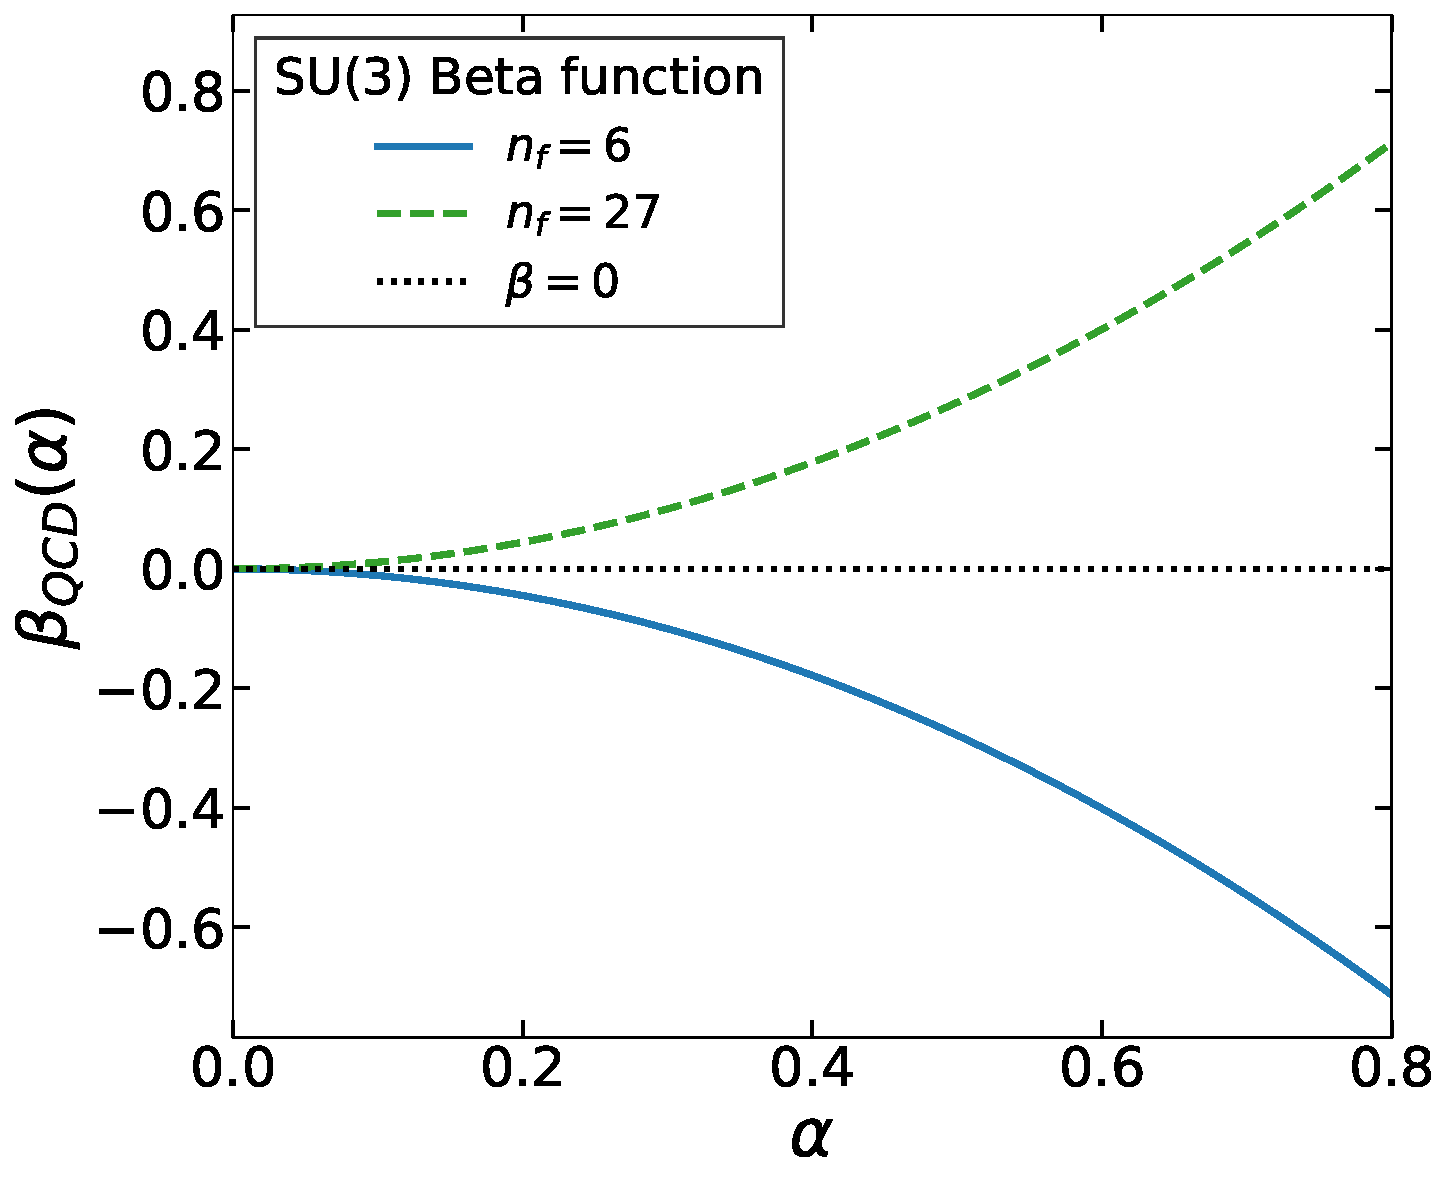
\includegraphics[width=\textwidth]{Figures/beta_function_alpha_pretty.pdf}
       \caption{QCD beta function}
       \label{fig:QCDBeta}
   \end{subfigure}
   \hspace{0.1cm}
   \begin{subfigure}[b]{0.49\textwidth}
       \centering
       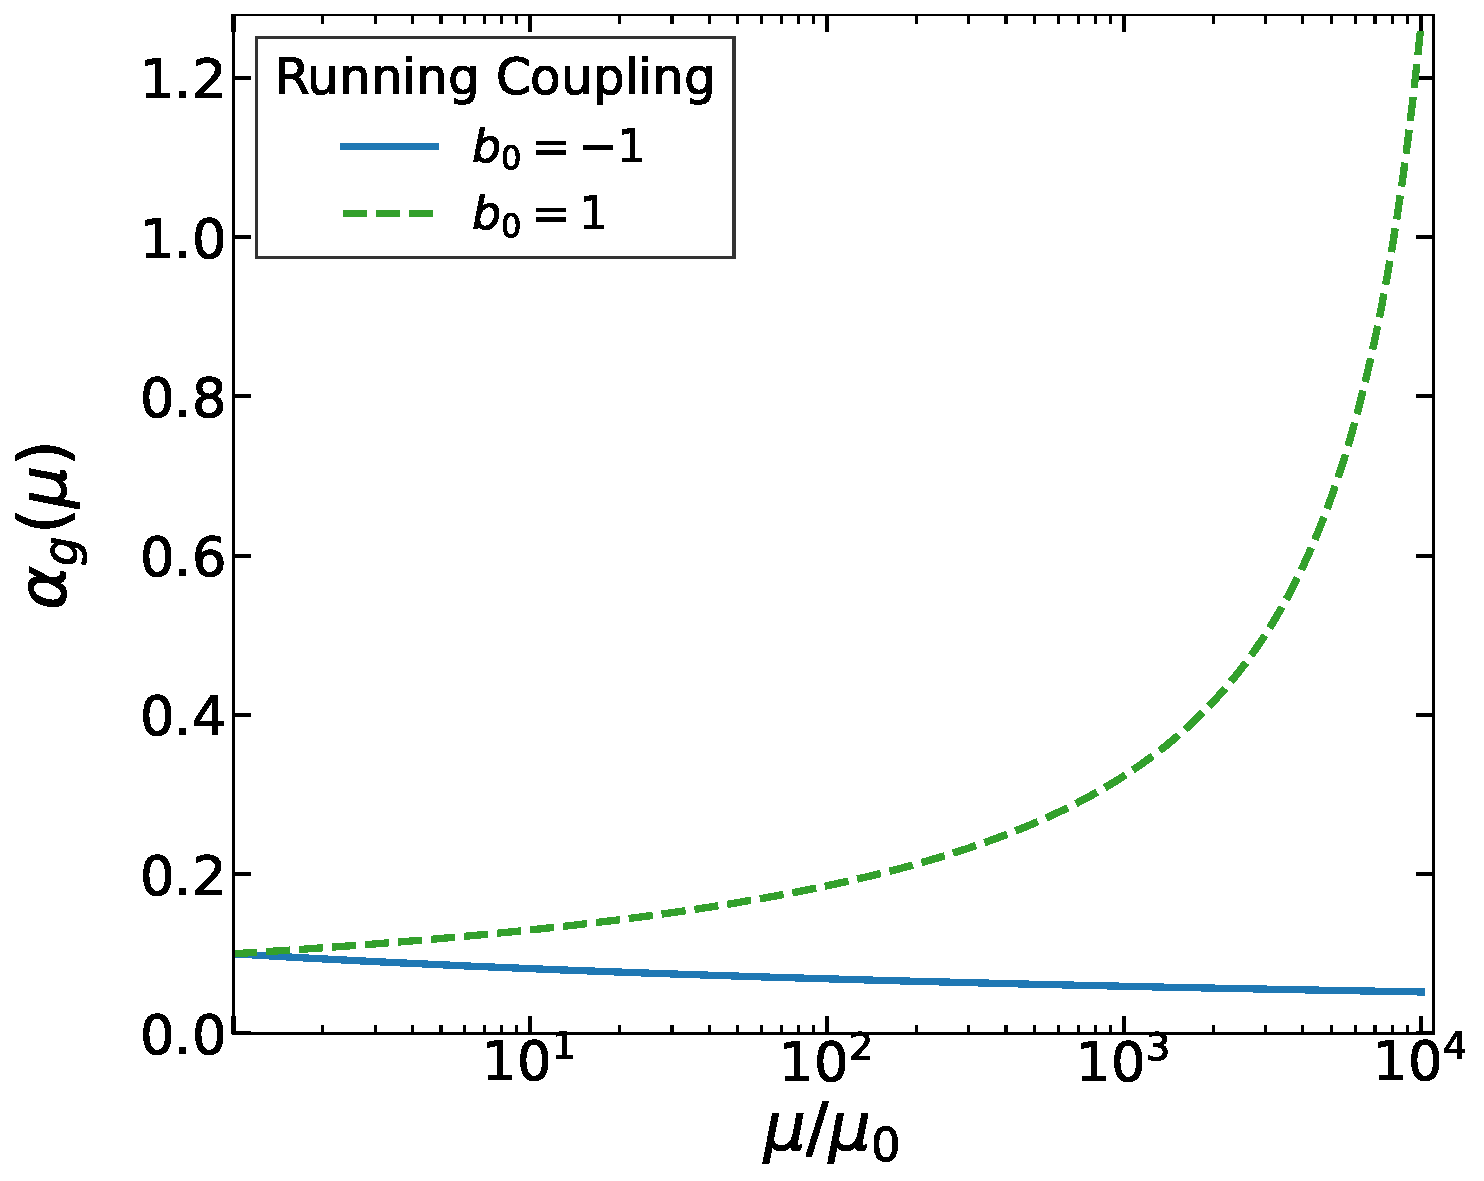
\includegraphics[width=\textwidth]{Figures/running_coupling_pretty-1.pdf}
       \caption{Running of coupling}
       \label{fig:runningcoupling}
   \end{subfigure}
   \caption{The $\SU(3)$ beta function and its corresponding solution. The left panel (A) displays the one-loop beta function for $n_f=6$ (solid blue) and $n_f=27$ (dashed green). The right panel (B) displays the running of the coupling for the two corresponding cases: negative $b_0$ (solid blue) and positive $b_0$ (dashed green).}
   \label{fig:betafunctheory}
\end{figure} 

To understand the dynamical behaviour of our couplings, we must find a solution to the corresponding beta function. We can do this by using separation of variables to solve the RG equation of the gauge coupling. We have the ordinary differential equation  
\begin{align}
    \mu\frac{\dd}{\dd\mu}\alpha_g=b_0\alpha_g^2\,,
\end{align}
where we can separate the variables and integrate
\begin{align}
    \frac{\dd\alpha_g}{\alpha_g^2}=\frac{\dd\ln(\mu)}{\mu}b_0\implies
    \int^{\alpha_g(\mu)}_{\alpha_g(\mu_0)}\frac{\dd\alpha_g}{\alpha_g}=b_0\int^{\mu}_{\mu_0}\frac{\dd\mu}{\mu}\,,
\end{align}
from which we obtain the solution  
\begin{align}
    \alpha_g=\frac{\alpha_{g_0}}{1-b_0 \alpha_{g_0} \ln \left(\frac{\mu}{\mu_0 }\right)}\,,
\end{align}
where $\alpha_{g_0}=\alpha_g(\mu_0)$ and $\mu_0$ is a chosen RG reference scale. The running of the coupling is depicted in Figure~\ref{fig:runningcoupling}, for the two non-trivial scenarios: $b_0>0$ and $b_0<0$. The former case implies a Landau pole at high energies, a characteristic of QED, and matches the fate of the dashed green trajectory in Figure~\ref{fig:QCDBeta}. The latter case demonstrates asymptotically freedom, where the blue solid line converges to zero at high energies, illustrating QCD behaviour.   

It will prove useful in Chapter \ref{chap:GUT} to consider the dependence on $\mu$ of the inverse coupling:
\begin{align}
    \alpha^{-1}_g(\mu)=\frac{1-b_0 \alpha_{g_0} \ln \left(\frac{\mu}{\mu_0 }\right)}{\alpha_{g}(\mu_0)}=\alpha_g^{-1}(\mu_0)-b_0\ln\frac{\mu}{\mu_0}\,.\label{eq:RGinversecoupling}
\end{align}
Now that we have reviewed the renormalisation group, beta functions, and asymptotic freedom, we can move onto discussing the SM and the motivations of GUTs. 
\chapter{Grand Unified Theories}
\label{chap:GUT}
This chapter expands our theoreitcal framework, beginning with an exploration of chiral theories. Because the SM is chiral, this provides the foundation needed to briefly review it in Section \ref{sec:SM}. Motivated by the shortcomings of the SM, we will motivate extenstions in Section \ref{sec:Motiv}, before considering the $\SU(5)$ GUT in Section \ref{sec:SU5} as an example.
\section{Chiral theories} \label{sec:chiral}
To understand the SM, we need to grasp understand \text{chirality}. This attribute of a theory arises from the Dirac equation 
\begin{equation}
    (i\gamma^\mu \partial_\mu - m)\psi (x) =0\;,
\end{equation}
where $\gamma^\mu$ is the gamma matrices. This can be rewritten, by moving to momentum space using the operator $\slashed{p}=\gamma^\mu(i\partial_\mu)$ and working in the Weyl representation, yields the matrix equation
\begin{equation}
\begin{pmatrix}
-m & p^0 - \vec{\sigma} \cdot \vec{p} \\
p^0 + \vec{\sigma} \cdot \vec{p} & -m
\end{pmatrix}
\begin{pmatrix}
\psi_L \\
\psi_R
\end{pmatrix}
= 0\;.
\end{equation}
The equation reveals that for massless particles the left- and right-handed Weyl spinors $\psi_L$ and $\psi_R$ do not mix \cite{Lancaster:2014}. For massless fermions, an additional symmetry also applies for the field, namely the chiral symmetry $\psi\to e^{i\gamma^5\phi}\psi$ \cite{Zee:2010}. 

In a \textit{chiral theory}, like the SM, the left- and right handed fermions transform differently under the gauge group. Consequently, you cannot combine left- and right-handed fermions to form a gauge-invariant mass term in the Lagrangian, such as 
\begin{equation}
    \mathcal{L}_{\text{mass}} = -m\bar{\psi}\psi = -m(\bar{\psi}_L\psi_R + \bar{\psi}_R\psi_L) \;,\label{eq:Chiralmass}
\end{equation}
Thus, in chiral theories, fermions obtain mass via spontaneous symmetry breaking (SSB), as in the Higgs mechanism (see Section \ref{sec:SMHiggs}).

\section{Standard Model} \label{sec:SM} 
Having established the implications of a chiral theory, we will in this section review the core components of the SM and motivate the work of physics beyond the Standard Model (BSM) particularly Grand Unified Theories (GUT)s. 

The SM is governed by two main types of symmetries. The first describes the symmetry of spacetime, which mathematically is described by the Lorentz and Poincaré group. The second of these is the gauge symmetry, which has the semi-simple group structure
\begin{equation}
    \mathcal{G}_{\mathrm{SM}}=\mathrm{SU}(3)_C\times\mathrm{SU}(2)_L\times\mathrm{U}(1)_Y\,,
\end{equation}
where the subscripts refer to $C$ colour, $L$ left, and $Y$ hypercharge. These indicates the defining properties of the group. The $\mathrm{SU}(3)_C$ describes the strong interaction \cite{Politzer:1973fx,Gross:1973id,Weinberg:1973un}, and $\mathrm{SU}(2)_L\times\mathrm{U}(1)_Y$ the electroweak interaction \cite{Glashow:1961tr,Salam:1964ry,Weinberg:1967tq}. The SM can be described by denoting the fields and thereby the particle content of the model, which transforms under these gauge groups. The conditions on the model are only that it adheres to Lorentz symmetry, the gauge symmetries $\mathcal{G}_{\mathrm{SM}}$, and renormalisability \cite{Pernow:2021fvb}. 

\subsection{Gauge bosons}
The gauge bosons are spin $1$ particles, and they act as the force carriers of the SM interactions. They are described by the generators of the gauge groups, such that each generator of a group corresponds to a gauge boson. The gauge bosons appear from promoting global symmetries to local and thus gauge symmetries \cite{Peskin:1995ev}. The SM gauge sector consists of three different gauge groups, where one is abelian $\U(1)_Y$, and two are non-abelian $\SU(2)_L$ and $\SU(3)_C$. The emergence of gauge bosons can be demonstrated by promoting a global symmetry to a local symmetry \cite{Pich:2007vu}. We will do this explicitly for abelian group $\U(1)$. 

The Lagrangian of a free Dirac field can be expressed as
\begin{align}
    \mathcal{L}=\bar\psi(i\gamma^\mu\partial_\mu-m)\psi\,,\label{eq:Lg}
\end{align}
where $\gamma^\mu$ are the Dirac matrices satisfying the Clifford algebra. This term is invariant under the global phase transformation
\begin{align}
    \psi\to\psi'=e^{-iq\alpha}\psi\,.
\end{align}
Since the phase angle $\alpha$ does not depend on spacetime coordinates, the derivative does not see the phase and only interacts with the fermion, leaving the Lagrangian unchanged. However, the invariance is lost if we promote the symmetry to be a local gauge transformation by allowing the phase angle to depend on spacetime
\begin{align}
    \psi\to\psi'=e^{-iq\alpha(x)}\psi\,.
\end{align}
Applying this local transformation does not leave the Lagrangian in Eq. \eqref{eq:Lg} invariant. Because of the spacetime dependence of the phase angle, the partial derivative yields two terms, given by
\begin{align}
    \partial_\mu \psi'=\partial_\mu\left(e^{-iq\alpha(x)}\psi\right)=e^{-iq\alpha(x)}\left(\partial_\mu\psi-iq(\partial_\mu \alpha(x)\psi)\right)\,.
\end{align}
Plugging this back into the Lagrangian, we obtain
\begin{align}
    \mathcal{L}'=\mathcal{L}+q(\partial_\mu \alpha(x)\psi)\,,
\end{align}
which breaks the gauge invariance of the Lagrangian. This can, however, be fixed by introducing a covariant derivative
\begin{align}
    D_\mu=\partial_\mu+iqA_\mu \,.\label{eq:Atrans}
\end{align}
To leave the covariant derivative of the Dirac field invariant the transformation rule of the gauge field needs to be $A_\mu\to A_\mu'=A_\mu+\partial_\mu\alpha(x)$. The field $A_\mu$ is the gauge field of the $\U(1)_Y$ group. To ensure that the field is dynamical, we need to include a kinetic term in the Lagrangian. This is constructed using the gauge-invariant field strength tensor $F_{\mu\nu}=\partial_\mu A_\nu-\partial_\nu A_\mu$. The full gauge invariant Lagrangian therefore reads 
\begin{align}
    \mathcal{L} = \bar{\psi}(i\slashed{D} - m)\psi - \frac{1}{4}F_{\mu\nu}F^{\mu\nu} = \bar{\psi}(i\slashed{\partial} - m)\psi - q\bar{\psi}\gamma^\mu\psi A_\mu-\frac{1}{4}F_{\mu\nu}F^{\mu\nu}\,.
\end{align}
 A similar approach can be followed for non-abelian groups, yielding an analogous result. However, there is one difference: The generators of non-abelian groups do not commute, hence, the gauge field exhibits self-interactions \cite{Yang:1954ek}. This self-coupling becomes explicit when we square the field strength tensor $F^a_{\mu\nu}$, resulting in terms proportional to
\begin{align}
    \mathcal{L}_{\mathrm{gauge,kin}}\supset (\partial_\mu A^a_\nu-\partial_\nu A^a_\mu)^2+gf^{abc}(\partial_\mu A^a_\nu)A^{\mu b}A^{\nu c}+g^2 f^{abc} f^{ade}A_{\mu}^{b}A_{\nu}^{c}A^{\mu d}A^{\nu e}\,.
\end{align}
The last two terms generate cubic and quartic self-interactions among the gauge bosons. This is a feature of the weak and strong interactions \cite{Pernow:2021fvb}. 

The SM is governed by the product gauge group $\mathrm{SU}(3)_C\times\mathrm{SU}(2)_L\times\mathrm{U}(1)_Y$. Demanding gauge invariance under all these three groups, give us the covariant derivative of the SM
\begin{align}
    D_\mu = \partial_\mu + ig_3 T^a G^a_\mu + ig_2 \tau^i W^i_\mu + ig_1 Y B_\mu\,,\label{eq:CovarD}
\end{align}
with the gauge fields
\begin{align}
    B_{\mu\nu} &= \partial_\mu B_\nu - \partial_\nu B_\mu, \\
    W_{\mu\nu}^i &= \partial_\mu W_\nu^i - \partial_\nu W_\mu^i + g_2 \epsilon^{ijk} W_\mu^j W_\nu^k, \\
    G_{\mu\nu}^a &= \partial_\mu G_\nu^a - \partial_\nu G_\mu^a + g_3 f^{abc} G_\mu^b G_\nu^c,\,,
\end{align}
where $B_\mu$ is the gauge boson of $\U(1)_Y$, $W_{\mu\nu}^i$ are the gauge bosons of $\SU(2)_L$, and $G_{\mu\nu}^a$ are the gauge bosons of $\SU(3)_C$. The generators of $\SU(2)_L$ correspond to $t^i=\frac{\sigma^i}{2}$ where $\sigma^i$ is the Pauli matrices and the superscript index is $i=1,2,3$ resulting in three gauge bosons. The generators of the strong interaction are $t^a=\frac{\lambda^a}{2}$ where $\lambda^a$ is the Gell-Mann matrices and $a=1,\dots,8$, and thus we have eight gauge bosons.

We can therefore write the gauge part of the Lagrangian as 
\begin{align}
    \mathcal{L}_{\mathrm{gauge}} = -\frac{1}{4} B_{\mu\nu} B^{\mu\nu} - \frac{1}{4} W_{\mu\nu}^i W^{i,\mu\nu} - \frac{1}{4} G_{\mu\nu}^a G^{a,\mu\nu}\,. \label{eq:LGauge}
\end{align}
Having now gone through the force carriers of the model, we can focus on the matter content.


\subsection{Fermionic matter}
In the SM model, the matter is composed of spin $1/2$ fermions, which we can categorise as either quarks or leptons. Furthermore, they come in three generations. We describe the particles by spinors, which can be decomposed into left- and right-handed components using the projection operators
\begin{align}
    P_{\mathrm{L}} = \frac{\mathds{1} - \gamma^5}{2}, \quad P_{\mathrm{R}} = \frac{\mathds{1} + \gamma^5}{2}\,,
\end{align}
where $\gamma^5=i\gamma^0\gamma^1\gamma^2\gamma^3$. The operators can be used to decompose the spinor, yielding 
\begin{align}
    \psi=P_L \psi+P_R\psi=\psi_L+\psi_R\,.
\end{align}
This is a crucial point since the SM is a chiral theory, which indicates that the two chiral components are treated differently in the SM. Mathematically, this means that the fermions transform differently under the gauge symmetry $\mathcal{G}_{\mathrm{SM}}$.

Let us first consider the quarks: They carry quantum numbers of all the three gauge groups, and transform as a fundamental. This means that quarks come in three colour charges: red, green, and blue. Because the fundamental representation of $\SU(3)_C$ is the $\mathbf{3}$ representation, we refer to it as a triplet under $\SU(3)_C$. Furthermore, the SM is a chiral theory, meaning that the $\SU(2)_L$ weak interaction exclusively couples to left-handed particles. Thus, right-handed quarks are singlets under $\SU(2)_L$ , and the left-handed quarks transform as doublets under $\SU(2)_L$ Consequently, we denote the quarks as
\begin{align}
    Q_{\mathrm{L}} = \begin{pmatrix} u_{\mathrm{L}}^c  \\ d_{\mathrm{L}}^c \end{pmatrix} \sim (\mathbf{3}, \mathbf{2})_{1/6}\,,\\
    u_{\mathrm{R}}^c  \sim (\mathbf{3}, \mathbf{1})_{2/3}\,,\qquad d_{\mathrm{R}}^c \sim (\mathbf{3}, \mathbf{1})_{-1/3}\,,
\end{align}
where $c=red,green,blue$. The representation under the gauge groups is denoted by $(p,q)_n$ where $p$ is the $p$-dimensional representation of the $\mathrm{SU}(3)_C$ group, $q$ is the $q$-dimensional representation of the $\mathrm{SU}(2)_L$ group, and finally the $n$ index denotes the charge under the $\mathrm{U}(1)_Y$ group. The hypercharge $Y=1/6$ stems from the SSB of the electroweak force, and will be explained in the following section. In the notation, the generation index is suppressed. The next generations follow a similar structure where $u$ and $d$ are replaced by $c$ and $s$ or $t$ and $b$. 

The leptons differ from the quarks because they do not have a colour charge and are thus singlets under $\SU(3)_C$. The left and right-handed components transform differently under $\SU(2)_L$, similar to the quarks. Additionally, there are no right-handed neutrinos. We can therefore organise the leptons as:
\begin{align}
    L_{\mathrm{L}} &= \begin{pmatrix} \nu_{e_\mathrm{L}} \\ e_{\mathrm{L}} \end{pmatrix} \sim (\mathbf{1}, \mathbf{2})_{-1/2}\,, \\
    \ell_\mathrm{R}&=e_{\mathrm{R}} \sim (\mathbf{1}, \mathbf{1})_{-1}\,.
\end{align}  
Again, the generation index is not written, but the next generations follow a similar structure where $e$ and $\nu_e$ are replaced by $\mu$ and $\nu_\mu$ or $\tau$ and $\nu_\tau$. 
We can now write the Dirac part of the Lagrangian as 
\begin{align}
    \mathcal{L}_{\mathrm{Dirac}} = i \overline{\Psi} \gamma^\mu D_\mu \Psi\,,\label{eq:LDirac}
\end{align}
where $\Psi$ are multiples containing all the fermions and the covariant derivative is given by Eq. \eqref{eq:CovarD}. 

With the matter and gauge sectors established, the next step will be to introduce mass terms. However, the chiral structure of $\SU(2)_L$ complicates this process and explicitly forbids including fermion mass terms in the Lagrangian (see Eq. \eqref{eq:Chiralmass}). 

The gauge fields are also massless. Recall the transformation rules of the gauge fields, defined in Eq. \eqref{eq:Atrans}, this makes mass terms $\sim m^2A_\mu A^\mu$ break gauge symmetries. This puzzle leads us to the Brout-Englert-Higgs mechanism \cite{Englert:1964et,Higgs:1964pj}. 

\subsection{The Higgs mechanism and Yukawa terms}
Particle masses in the SM are generated through SSB of the electroweak group, as described by the Glashow--Weinberg--Salam theory \cite{Glashow:1961tr, Weinberg:1967tq, Salam:1964ry}. The mechanism responsible for this was first proposed by Brout, Englert and Higgs in the 1960's \cite{Englert:1964et,Higgs:1964pj}. Decades later in 2012 the particle responsible for this mechanism, the Higgs, was found experimentally by ATLAS \cite{ATLAS:2012yve} and CMS \cite{CMS:2012qbp} collaborations. 

The Higgs is a singlet under $\SU(3)_C$ and a doublet under $\SU(2)_L$ with a hypercharge $Y=1/2$ \cite{Georgi:1999wka}. We thus have a complex scalar, on the form
\begin{align}
    \Phi = \begin{pmatrix} \phi^+ \\ \phi^0 \end{pmatrix} = \frac{1}{\sqrt{2}} \begin{pmatrix} \phi_1 + i\phi_2 \\ \phi_3 + i\phi_4 \end{pmatrix} \sim (\mathbf{1}, \mathbf{2})_{1/2}\,,\label{eq:Higgs1}
\end{align}
where $\psi^+$ indicates an electrically positively charged component, and $\phi^0$ a neutral. 

It has both a kinetic and a potential term in the Lagrangian 
\begin{align}
    \mathcal{L}_{\mathrm{Higgs}} = (D_\mu \Phi)^\dagger (D^\mu \Phi) - V(\Phi)\,.\label{eq:LHiggs}
\end{align}
The potential being the most general renormalisable potential, which takes the form:
\begin{align}
    V(\Phi) = -\mu^2 (\Phi^\dagger \Phi) + \frac{\lambda}{4} (\Phi^\dagger \Phi)^2.
\end{align}
The minus in front of the first term ensures that the potential has the famous Mexican hat shape \comment{add plot}. This further ensures that the minimum is not given by $\Phi=0$, but rather this will be an unstable local maximum. 
\begin{figure}[htbp]
    \centering
    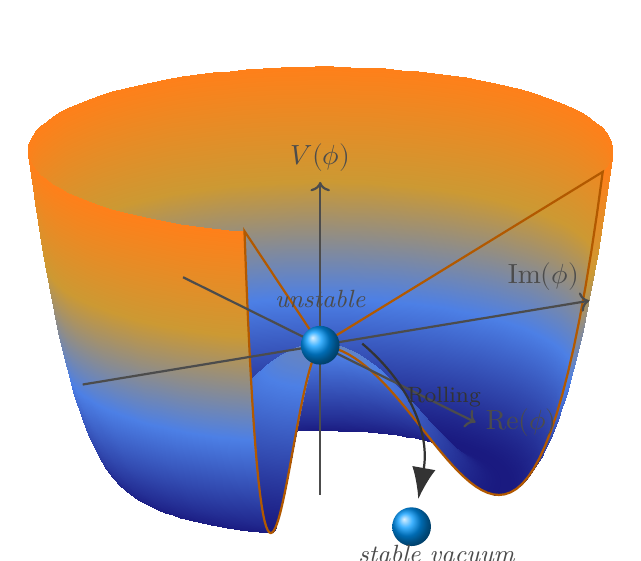
\begin{tikzpicture}
    \begin{axis}[
        view={60}{30},
        axis lines=none,
        width=13cm,
        height=9cm,
        colormap={viridis-like}{
            rgb(0)=(0.1,0.1,0.5)
            rgb(1)=(0.3,0.5,0.9)
            rgb(2)=(0.8,0.6,0.2)
            rgb(3)=(1,0.5,0.1)
        },
        xmin=-1.8, xmax=1.8,
        ymin=-1.8, ymax=1.8,
        zmin=-1.2, zmax=1.2,
        clip=false
    ]

    % Surface with cutout from 315° to 45° (i.e., missing a 90° wedge)
    \addplot3[
        surf,
        domain=45:315,         % missing wedge from 315° to 45° (across 0°)
        y domain=0:1.6,
        samples=80, samples y=40,
        z buffer=sort,
        shader=interp,
        faceted color=black!30,
    ] ({y*cos(x)}, {y*sin(x)}, {y^4 - 2*y^2});

    % Thick edges along the cut boundaries
    \addplot3[thick, orange!70!black, domain=0:1.6, samples=50]
        ({x*cos(45)}, {x*sin(45)}, {x^4 - 2*x^2});
    \addplot3[thick, orange!70!black, domain=0:1.6, samples=50]
        ({x*cos(315)}, {x*sin(315)}, {x^4 - 2*x^2});

    % Axes
    \draw[->, thick, black!70] (axis cs: 0,0,-1.1) -- (axis cs: 0,0,1.2) node[above] {$V(\phi)$};
    \draw[->, thick, black!70] (axis cs:-1.5,0,0) -- (axis cs:1.7,0,0) node[right] {$\operatorname{Re}(\phi)$};
    \draw[->, thick, black!70] (axis cs:0,-1.5,0) -- (axis cs:0,1.7,0) node[above left] {$\operatorname{Im}(\phi)$};

    % Balls with larger size and better shading
    \node[circle, shading=ball, ball color=cyan!60!blue, minimum size=14pt] at (axis cs:0,0,0) {};
    \node[circle, shading=ball, ball color=cyan!60!blue, minimum size=14pt] at (axis cs:1.0,0,-1) {};

    % Rolling arrow with a more curved path
    \draw[->, thick, black!80, -{Latex[length=4mm]}, bend left=30]
        (axis cs:0.2,0.15,0.05) to (axis cs:0.9,0.1,-0.85);
    \node[black!80, font=\footnotesize, anchor=south west] at (axis cs:0.5,0.2,-0.4) {Rolling};

    % Labels
    \node[font=\small\itshape, black!70, anchor=south] at (axis cs:0,0,0.2) {unstable};
    \node[font=\small\itshape, black!70, anchor=north] at (axis cs:1.1,0.1,-1.05) {stable vacuum};

    \end{axis}
    \end{tikzpicture}   
    \caption{The Higgs potential $V(\Phi)$ with a section removed to reveal the inner structure. The blue spheres represent the scalar field, showing the transition from the unstable symmetric state ($V=0$) to the stable broken-symmetry vacuum state.}
    \label{fig:mexican_hat_balls}
\end{figure}
To find the minimum, we minimise the potential 
\begin{align}
    \frac{\partial V}{\partial(\Phi^\dagger \Phi)} = -\mu^2 + \frac{\lambda}{2} \Phi^\dagger \Phi\,,
\end{align}
which yields the minimum 
\begin{align}
    (\Phi^\dagger \Phi)_{\min} = \frac{2\mu^2}{\lambda}.
\end{align}
The vacuum expectation value (VEV) of the Higgs can now be chosen along the $\phi^0$ direction (see Eq. \eqref{eq:Higgs1}) \cite{Pernow:2021fvb}. This choice ensures that the vacuum remains neutral, resulting in the VEV
\begin{align}
    \langle \Phi \rangle = \sqrt{\frac{2\mu^2}{\lambda}} \equiv \frac{1}{\sqrt{2}}\begin{pmatrix}
        0\\v
    \end{pmatrix}\,,\label{eq:VEVhiggs}
\end{align}
where $v=\sqrt{4\mu^2/\lambda}$.
Having defined the VEV, we can asses the influence on the electroweak gauge group. This is necessary to learn what symmetries are broken, and if any survives. Consider the general transformation of the Higgs field
\begin{align}
    \Phi \rightarrow \Phi' = e^{i\alpha^a T^a} e^{i\beta/2} \Phi\,,
\end{align}
where $T^a=\sigma^a/2$. For the specific parameter values $\alpha^1=\alpha^2=0$ and $\alpha^3=\beta$ \cite{Peskin:1995ev} this results in
\begin{align}
\Phi \rightarrow \Phi'&=\exp \left[ i \beta T^3 + i \beta / 2 \right] \Phi \\
&= \exp \left\{ i \beta \left[ \frac{1}{2} \begin{pmatrix} 1 & 0 \\ 0 & -1 \end{pmatrix} + \begin{pmatrix} 1/2 & 0 \\ 0 & 1/2 \end{pmatrix} \right] \right\} \Phi \\
&= \exp \left[ i \beta \begin{pmatrix} 1 & 0 \\ 0 & 0 \end{pmatrix} \right] \Phi \,.
\end{align}
We can now insert the VEV from Eq. \eqref{eq:VEVhiggs} into the expression, which yields
\begin{align}
    \Phi'= \begin{pmatrix} e^{i\beta} & 0 \\ 0 & 1 \end{pmatrix} \frac{1}{\sqrt{2}} \begin{pmatrix} 0 \\ v \end{pmatrix} = \frac{1}{\sqrt{2}} \begin{pmatrix} 0 \\ v \end{pmatrix}\,.\label{eq:VEVinvariant}
\end{align}
Because the VEV is unchanged by the symmetry generated by this specific parameter combination ($Q=T^3+Y$) is not broken by the vacuum. Thus, the gauge boson, associated with this symmetry, the photon, will remain massless. This combination is the only possible combination which will leave the VEV invariant under the gauge transformation \cite{Peskin:1995ev}. The remaining three gauge bosons will thus gain mass. 

We can write the SSB as
\begin{align}
    \SU(2)_{\mathrm{L}} \times \U(1)_{Y} \rightarrow \U(1)_{Q}\,,
\end{align}
where the surviving generator is given by the Gell-Mann Nishijima formula \cite{Gell-Mann:1956iqa,Nishijima:1955gxk} 
\begin{align}
    Q=T^3+Y\,,\label{eq:chargedef}
\end{align}
which is the same generator that left the VEV invariant, as shown in Eq. \eqref{eq:VEVinvariant}.

During the SSB, we have lost three degrees of freedom, these are the so-called \textit{Goldstone bosons} \cite{Goldstone:1961eq,Goldstone:1962es}. These become evident when expanding around the VEV \cite{Pernow:2021fvb}
\begin{align}
    \Phi = \frac{1}{\sqrt{2}} \begin{pmatrix} \phi_1+i\phi_2 \\ v + h + i\sigma \end{pmatrix}\,,
\end{align}
where $\phi_1,\phi_2$, and $\sigma$ is the Goldstone bosons, and $h$ is the Higgs. The gauge bosons corresponding to the broken generators \textit{eat} the Goldstone bosons. By absorbing the scalar fields the gauge bosons acquire a longitudinal degree of freedom, effectively acquiring mass \cite{Pernow:2021fvb}. 

This can also be visualisation of this can be found in Figure \ref{fig:mexihat}. A change along the radial component, allow us to "climb" up the potential wall, corresponding to a massive Higgs boson. However, rotations around the bottom of the hat, requires no extra energy, giving rise to the massless Goldstone bosons ($\phi_1,\phi_2$, and $\sigma$). 

\paragraph{Gauge boson masses: } The mass of the gauge bosons come from the kinetic term of the Higgs field, where the covariant derivative of the VEV is 
\begin{align}
D_\mu \Phi &= \left( \partial_\mu - i g_2 W_\mu^a \tau^a - i \frac{1}{2} g_1 B_\mu \right) \Phi \\D_\mu \langle\Phi\rangle\implies
&= -i \left( g_2 W_\mu^a \frac{\sigma^a}{2} + g_1 \frac{1}{2} B_\mu \right) \frac{1}{\sqrt{2}} \begin{pmatrix} 0 \\ v \end{pmatrix} \,,\label{eq:gmass}
\end{align}
where the derivative of the VEV vanishes. Inserting the Pauli matrices, the first term simplifies to
\begin{align}
    g_2 W_\mu^a \frac{\sigma^a}{2} &= \frac{g_2}{2} \left[ W_\mu^1 \begin{pmatrix} 0 & 1 \\ 1 & 0 \end{pmatrix} + W_\mu^2 \begin{pmatrix} 0 & -i \\ i & 0 \end{pmatrix} + W_\mu^3 \begin{pmatrix} 1 & 0 \\ 0 & -1 \end{pmatrix} \right] \\
&= \frac{g_2}{2} \begin{pmatrix} W_\mu^3 & W_\mu^1 - i W_\mu^2 \\ W_\mu^1 + i W_\mu^2 & -W_\mu^3 \end{pmatrix} \,.\label{eq:1g}
\end{align}
The second term of Eq. \eqref{eq:gmass} is given by
\begin{align}
    g_1 \frac{1}{2} B_\mu &= \frac{g_1}{2} \begin{pmatrix} B_\mu & 0 \\ 0 & B_\mu \end{pmatrix} \,.\label{eq:2g}
\end{align}
Combining the terms from Eq. \eqref{eq:1g} and \eqref{eq:2g}, we obtain the covariant derive of the VEV 
\begin{align}
   D_\mu \langle\Phi\rangle= -i \frac{1}{2\sqrt{2}} &\begin{pmatrix} g_2 W_\mu^3 + g_1 B_\mu & g_2 (W_\mu^1 - i W_\mu^2) \\ g_2 (W_\mu^1 + i W_\mu^2) & -g_2 W_\mu^3 + g_1 B_\mu \end{pmatrix} \begin{pmatrix} 0 \\ v \end{pmatrix} = -i \frac{v}{2\sqrt{2}} \begin{pmatrix} g_2 (W_\mu^1 - i W_\mu^2) \\ -g_2 W_\mu^3 + g_1 B_\mu \end{pmatrix}\,.
\end{align}
From this, we can construct the kinetic terms of the Higgs field, given by
\begin{align}
\mathcal{L}_{\mathrm{Higgs, kin}} &= \frac{v^2}{8} \left[ g_2^2 (W_\mu^1 - i W_\mu^2)(W^{1\mu} + i W^{2\mu}) + (-g_2 W_\mu^3 + g_1 B_\mu)^2 \right] \\
&= \frac{v^2}{8} \left[ g_2^2 W_\mu^1 W^{1\mu} + g_2^2 W_\mu^2 W^{2\mu} + (-g_2 W_\mu^3 + g_1 B_\mu)^2 \right]\,,
\end{align}
We can thus write the massive gauge bosons as \cite{Peskin:1995ev}
\begin{align}
    W_\mu^\pm &= \frac{1}{\sqrt{2}} (W_\mu^1 \mp iW_\mu^2), \quad Z_\mu^0 = \frac{1}{\sqrt{g_1^2 + g_2^2}} (g_2 W_\mu^3 - g_1 B_\mu)\,,
    \\M_W &= \frac{g_2 v}{2}, \quad M_Z = \sqrt{g_1^2 + g_2^2} \frac{v}{2}\,,
\end{align}
and the massless mode as 
\begin{align}
    A_\mu = \frac{1}{\sqrt{g_1^2 + g_2^2}} (g_1 W_\mu^3 + g_2 B_\mu)\,,
\end{align}
where $A_\mu$ represents the photon, $W^{\pm}_\mu$ are the two charged force carriers of the weak interaction, and $Z^0_\mu$ is the neutral gauge boson. 
Further, the Weinberg angle \cite{Pernow:2021fvb} can be defined 
\begin{align}
    \tan\theta_w=\frac{g_1}{g_2}\,,
\end{align}
where the masses of the gauge bosons are related through the angle as \cite{Peskin:1995ev}
\begin{align}
    \frac{M_W}{M_Z}=\cos\theta_w\,.
\end{align}
Now that the gauge bosons responsible for the weak interaction have received a mass, we can redirect our focus to the fermions.

\paragraph{Hypercharge of fermions: }Let us first consider the hypercharges as previously promised. Right-handed fermions transform as singlets under the weak interaction, thus the have an isopsin of zero. According to the Gell--Mann--Nishijima relation (see Eq. \eqref{eq:chargedef}), this reduces to the condition $Y=Q$. Conversely, the left-handed fermions transform as doublets under $\SU(2)_L$, carrying an isospin of $\pm1/2$. The left-handed neutrinos and up quarks will have positive isospin, while electrons and down quarks have negative isospin.  

We can use Eq. \eqref{eq:chargedef} to compute the hypercharge, using the isospin of the different particles, which yields 
\begin{align}
L_L &= \begin{pmatrix} \nu_{eL} \\ e_L \end{pmatrix}_{-1/2} \,,\\
Q_L &= \begin{pmatrix} u_L \\ d_L \end{pmatrix}_{1/6} \,,
\end{align}
where the subscript denotes the hypercharge. These specific assignments ensures the familiar charges: neutrinos are neutral, electrons have $Q=-1$, up quarks $Q=+2/3$, and down quarks $Q=-1/3$. 

\paragraph{Fermion masses: } Having established the hypercharges of the fermions, we can now address the mass generation for the fermions. 

The generation of masses stems from the Yukawa terms in the Lagrangian. These can be written, because of the addition of a scalar into our theory. The Yukawa terms combine two fermions and one scalar, for the SM they are given by
\begin{align}
    \mathcal{L}_{\mathrm{Yukawa}} = -y_d^{\gamma\delta} \overline{Q_{\mathrm{L}}^\gamma} \Phi d_{\mathrm{R}}^\delta - y_u^{\gamma\delta} \overline{Q_{\mathrm{L}}^\gamma} \tilde{\Phi} u_{\mathrm{R}}^\delta - y_\ell^{\gamma\delta} \overline{L_{\mathrm{L}}^\gamma} \Phi \ell_{\mathrm{R}}^\delta + \mathrm{h.c.}\,,\label{eq:LYukawa}
\end{align} 
where we have introduced the generation index $\gamma,\delta=(1,2,3)$ and $y_d,\,y_u,\,y_\ell$ represent the $3\times3$ Yukawa matrices. 

The first term couples the right-handed down-type quarks with the left-handed quarks. Similarly, the third term relates the right-handed electrons with the left-handed leptons. Lastly, the second term relates the right-handed up quarks with the left-handed quarks by introducing $\tilde\Phi=i\sigma_2\Phi^*$. The $\tilde\Phi$ rotates the VEV (Eq. \eqref{eq:VEVhiggs}) such that the particles of isospin $1/2$ also acquire mass. 

When the Higgs field acquires the VEV, the fermion mass is given by the minimum of the Higgs potential (see Eq. \eqref{eq:VEVhiggs}) multiplied by the Yukawa matrix
\begin{align}
    M_d = Y_d \frac{v}{\sqrt{2}}\,, \quad M_u = Y_u \frac{v}{\sqrt{2}}\,, \quad M_\ell = Y_\ell \frac{v}{\sqrt{2}}\,.
\end{align}
To ensure that the Yukawa matrices describe physical mass eigenstates the mass matrices needs to be diagonalised using the unitary operators \cite{Pernow:2021fvb}. We need two types of unitary operators, for the difference in chirality, yielding
\begin{align}
    M_d = U_{d_{\mathrm{L}}}^\dagger \tilde{M}_d U_{d_{\mathrm{R}}}, \quad M_u = U_{u_{\mathrm{L}}}^\dagger \tilde{M}_u U_{u_{\mathrm{R}}}, \quad M_\ell = U_{\ell_{\mathrm{L}}}^\dagger \tilde{M}_\ell U_{\ell_{\mathrm{R}}}\,,
\end{align}
where $\tilde{M}$ is the diagonalised mass matrices. Writing the fermionic fields in this basis, yields 
\begin{align}
(d'_{\mathrm{L}})^i &= (U_{d_{\mathrm{L}}})^{ij}(d_{\mathrm{L}})^j\,, \quad (d'_{\mathrm{R}})^i = (U_{d_{\mathrm{R}}})^{ij}(d_{\mathrm{R}})^j\,, \\
(u'_{\mathrm{L}})^i &= (U_{u_{\mathrm{L}}})^{ij}(u_{\mathrm{L}})^j\,, \quad (u'_{\mathrm{R}})^i = (U_{u_{\mathrm{R}}})^{ij}(u_{\mathrm{R}})^j\,, \\
(L'_{\mathrm{L}})^i &= (U_{\ell_{\mathrm{L}}})^{ij}(L_{\mathrm{L}})^j\,, \quad (\ell'_{\mathrm{R}})^i = (U_{\ell_{\mathrm{R}}})^{ij}(\ell_{\mathrm{R}})^j\,.
\end{align}
This gives rise to observable physical consequences, which manifests in the kinetic term of the fermions. Let us consider the dynamic term of the left-handed quark doublet
\begin{align}
    \mathcal{L} \supset i \overline{Q}_L \gamma^\mu D_\mu Q_L \supset \frac{g_2}{2} \begin{pmatrix} \overline{u}_L & \overline{d}_L \end{pmatrix} \gamma^\mu \sigma^a W_\mu^a \begin{pmatrix} u_L \\ d_L \end{pmatrix}\,.
\end{align} 
The off-diagonal terms of the first two Pauli matrices result in mixing of $\bar{u}_L$ and $d_L$. In the basis where $u'_\mathrm{L}=U_{u_{\mathrm{L}}}u_\mathrm{L}$ and $d'_\mathrm{L}=U_{d_{\mathrm{L}}}d_\mathrm{L}$, the mixing results in 
\begin{align}
    \overline{u}'_L U^\dagger_{u_L} \gamma^\mu U_{d_L} d'_L \,,\label{eq:CKMLterm}
\end{align}
from which the Cabibbo--Kobayashi--Maskawa (CKM) matrix \cite{Cabibbo:1963yz,Kobayashi:1973fv} is defined
\begin{align}
    V_{\mathrm{CKM}} = U_{u_{\mathrm{L}}} U_{d_{\mathrm{L}}}^\dagger\,.
\end{align}
The dimensions of the matrix depends on the generations of the matter particles. Let us first consider the case of two generations. 

For two generations, the matrix has four degrees of freedom: three phases and one angle. As there are four available quarks, all three phases can be absorbed by the quarks by performing phase rotations of three of the quark fields \cite{Peskin:1995ev}. Note that we cannot perform phase rotations for all quark fields, as this would simply cancel out and not absorb any phases\footnote{Consider the general Lagrangian term $\overline{u}_i V_{ij} d_j$, if we shift the quarks with a global phase $d_i\to e^{i\theta_i}d_i$ and $u_i\to e^{i\phi_i}u_i$. The CKM matrix is only affected by the difference of the phases and since the exponent yields a global phase. Thus, no phase is absorbed. This is a global $U(1)$ symmetry, which ensures preservation of baryon number\cite{Pernow:2021fvb}. }. This implies that the $\mathcal{CP}-$symmetry is not violated with two generations, since the mixing matrix is real. Only for a real mixing matrix would a $\mathcal{CP}-$transformation leave the terms involving the CKM matrix invariant. Thus, a complex mixing matrix breaks $\mathcal{CP}-$symmetry. 

In the SM, we have a $\mathcal{CP}-$violation, which was first discovered in 1964 through decays of neutral kaons \cite{Christenson:1964fg}. This forces us to introduce at least one extra generation to ensure CP violation, which was the motivation originally for the CKM matrix \cite{Cabibbo:1963yz,Kobayashi:1973fv}. It was only later that the third generation was discovered experimentally. 

The difference between two and three generations is that we cannot remove all the phases in the CKM matrix by phase rotation of the quark fields. For three generations, there would be nine degrees of freedom, where three would be rotation angles, and six would be phases. This time, we have six available quark fields, and therefore, it will only be possible to remove five of the phases from the CKM matrix. The remaining phase will therefore be responsible for $\mathcal{CP}-$violation.

\subsection{The SM and problems}
After going through the different components of the SM, we can write the Lagrangian of the SM as 
\begin{align}
    \mathcal{L}_{\mathrm{SM}} = \mathcal{L}_{\mathrm{gauge}} + \mathcal{L}_{\mathrm{Dirac}} + \mathcal{L}_{\mathrm{Higgs}} + \mathcal{L}_{\mathrm{Yukawa}}\,,
\end{align}
where the different terms can be found in Eq. \eqref{eq:LGauge}, \eqref{eq:LDirac}, \eqref{eq:LHiggs}, and \eqref{eq:LYukawa}. 

Now that we have briefly considered the different parts and parameters of the SM, we can count the number of parameters in the Lagrangian: There are 3 gauge couplings, the Weinberg angle, the Higgs VEV and its quartic coupling, 9 Yukawa couplings of the quarks and leptons, and 4 CKM parameters (3 rotation angles and one phase). Summing this up we arrive at 19 parameters, which seems like a lot of parameters for a minimal elementary model \cite{Pernow:2021fvb}. The complete particle content of the SM can be seen in Table \ref{tab:SMparticle}.

\begin{table}[h]
\centering
\renewcommand{\arraystretch}{1.8} 
\begin{tabular}{llcccc}
\toprule
\textbf{Category} & \textbf{Field} & \textbf{Hypercharge ($Y$)} & \textbf{Representation} & \textbf{Charge ($Q$)} \\
\midrule
\textbf{Gauge Bosons} & $B_\mu$ & 0 & $(\mathbf{1}, \mathbf{1})_0$ & 0 \\
                      & $W_\mu$ & 0 & $(\mathbf{1}, \mathbf{3})_0$ & $0, \pm 1$ \\
                      & $G_\mu$ & 0 & $(\mathbf{8}, \mathbf{1})_0$ & 0 \\
\midrule
\textbf{Fermions}     &  & & & \\
\textit{Leptons}      & $L_{\text{L}}^i$    & $-1/2$ & $(\mathbf{1}, \mathbf{2})_{-1/2}$ & $0, -1$ \\
                      & $\ell_{\text{R}}^i$ & $-1$   & $(\mathbf{1}, \mathbf{1})_{-1}$   & $-1$ \\
\cline{2-5} % Adjusted line coordinates to match the new column count (columns 2 to 5)
\textit{Quarks}
                      & $Q_{\text{L}}^i$    & $1/6$  & $(\mathbf{3}, \mathbf{2})_{1/6}$  & $2/3, -1/3$ \\
                      & $u_{\text{R}}^i$    & $2/3$  & $(\mathbf{3}, \mathbf{1})_{2/3}$  & $2/3$ \\
                      & $d_{\text{R}}^i$    & $-1/3$ & $(\mathbf{3}, \mathbf{1})_{-1/3}$ & $-1/3$ \\
\midrule
\textbf{Scalar Boson} & $\Phi$ & $1/2$  & $(\mathbf{1}, \mathbf{2})_{1/2}$ & $1, 0$ \\
\bottomrule
\end{tabular}
\caption{Particle content of the Standard Model including their representation under $\mathcal{G}_{\mathrm{SM}}$ and their charges.}
\label{tab:SMparticle}
\end{table}

Despite the SM's predictive abilities, the SM still suffers from some challenges \cite{Pernow:2021fvb}. We will briefly mention these here: 
\begin{itemize}
    \item \textbf{Neutrinos are massless} in the SM, since we cannot write down a mass term without a right-handed neutrino. Consequently, the neutrinos should not be able to change flavour. This prediction of the SM, is directly in conflict with the observations of neutrino oscillations \cite{Pontecorvo:1967fh}. Therefore, a complete theory of particle physics would have to include an explanation of the mass generation of the neutrinos.
    \item \textbf{Missing description of dark matter} which has been predicted through cosmological \cite{WMAP:2012fli,Planck:2018vyg} and astrophysical \cite{Zwicky:1933gu,Rubin:1970zza, Clowe:2006eq} observations. From these it is estimated that the around $25\%$ of the content in the Universe consists of dark matter \cite{Planck:2018vyg}. None of the particles in the SM is dark matter candidates, and thus to find dark matter particles one has to search for physics beyond the SM \cite{Pernow:2021fvb}.
    \item \textbf{Gravity} is not described by the SM. Thus, a successful, truly fundamental theory would also have to include a quantum description of gravity.
    \item \textbf{Matter-antimatter asymmetry} is a well known puzzle. The fact that the Universe manly consists of matter requires a violation of baryon number, $\mathcal{C}$- and $\mathcal{CP}$-symmetry, and out-of-equilibrium interactions \cite{Sakharov:1967dj}. Baryon number is violated \cite{Kuzmin:1985mm}. The $\mathcal{C}$-symmetry is maximally violated in the weak sector, and that $\mathcal{CP}$-symmetry is violated through the CKM matrix. However, the violation of $\mathcal{CP}$-symmetry is not strong enough to explain the ratio of baryon to photons \cite{Gavela:1993ts}. Lastly, the out-of-equilibrium condition is not satisfied through the smooth phase transition at the electroweak scale \cite{Kajantie:1996mn}. 
    \item \textbf{Charge assignments} in the SM, the hypercharges of the quarks and leptons are assigned arbitrary values. However, these values are chosen in such a way that the anomalies\footnote{Classical symmetries which are not conserved in QFT results in an \textit{anomaly} \cite{Bilal:2008qx}. Even though the term anomaly suggest a fault of the theory \cite{Zee:2010} in a global symmetry it makes processes which are not possible at the classical level possible at the quantum level. However, an anomaly in a gauge symmetry is detrimental to the theory and breaks unitarity \cite{Bilal:2008qx}.} precisely cancel \cite{Adler:1969gk,Bell:1969ts,Pernow:2021fvb}. There is no explanation in the SM why the charges are perfectly chosen to cancel. Additionally, there is no reason why the charge of the proton (composite particle composed of three quarks) is exactly equal to and opposite to that of the electron (lepton).
    \item \textbf{The flavour puzzle} is related to the origin of the generations. The masses of the fermions are hierarchical and span multiple orders of magnitude through the three generations. The CMK matrix is almost diagonal, working against mixing of the different generations of quarks, whereas the mixing of leptons is more probable due to the similar size of the mixing elements. All this is encapsulated in the so-called flavour puzzle \cite{Feruglio:2015jfa}. 
    \item \textbf{Naturalness} describes the issue of the need to fine tune parameters in the SM. The Higgs mass has been measured to be $125\,$GeV \cite{ATLAS:2012yve,CMS:2012qbp}. However, a well-known problem arises, when adding a scalar into the theory: The mass will be affected by large quantum corrections \cite{Gaillard:1998ui}. The scale of the mass of the Higgs is low compared to the Planck scale at $10^{19}\,$GeV. If the SM is valid up until this scale, the quantum corrections should increase the Higgs mass to that scale \cite{Susskind:1978ms,Vieira:2012ex}. Thus, to give the Higgs particle its low mass, one needs to subtract two numbers with a precision of 30 digits. This is one part of the naturalness problem. \\
    Another parameter which requires fine-tuning in the SM relates to the strong $\mathcal{CP}$ problem \cite{tHooft:1976rip,tHooft:1976snw,Wilczek:1977pj}. This problem arises from a topological term in the Lagrangian, with a physical implication of the introduction of an electric dipole moment of the neutron \cite{Sannino:2026wgx} through the parameter $\theta$. However, experimental observations impose an upper bound of $|\theta|\le 10^{-10}$ \cite{Abel:2020pzs}. The small size of the angle cannot be explained by the particle content of the SM\footnote{A possible solution to this is the addition of an axion field \cite{Peccei:1977hh,Peccei:1977ur,}, which could also possibly explain dark matter \cite{Preskill:1982cy, Abbott:1982af,Dine:1982ah}. However, such a field is yet to be discovered experimentally \cite{ParticleDataGroup:2024cfk}.} and thus requires fine-tuning \cite{Pernow:2021fvb}.   
\end{itemize}

These challenges suggest that the SM is an effective field theory, only valid a low energies. Further, they motivate physics beyond the SM (BSM) to address these shortcomings. A branch of BSM physics explores the idea of unification of the three forces at some energy scale. This type of framework and the motivation for it will be examined in the next section.

\section{Motivation of Standard Model extensions}\label{sec:Motiv}
Grand Unified Theories (GUT)s aim to resolve some of the shortcomings of the SM by unifying the three gauge groups to a single gauge group at some energy above the energy scale $M_\mathrm{GUT}$ \cite{Langacker:1994vf}. At this scale, the GUT would break down to the gauge groups of the SM, so that at low energies, the effective particle model describing our universe would be the SM. This scale $M_X$ would have to be below the Planck scale $M_p\sim G_N^{-1/2}\sim10^{19}\,$GeV and at a scale where the gauge couplings meet \cite{Georgi:1974yf}.  

The motivation for GUTs is also often made by plotting the inverse gauge coupling and observing that they intertwine at high energies around $10^{13}-10^{17}\,$GeV. This can be demonstrated explicitly by utilising Eq. \eqref{eq:RGinversecoupling}, which describes the running of the gauge couplings
\begin{align}
    \alpha^{-1}_{g_i}(\mu)=\alpha_{g_i}^{-1}(\mu_0)-b_{0_i}\log\frac{\mu}{\mu_0}\,,
\end{align}
where the $i$ index runs over the three couplings of the SM. First, we need values of the couplings at a certain energy scale $\alpha_{g_i}^{-1}(\mu_0)$. A convenient choice is the electroweak scale\footnote{Given by the mass of the Z-boson.} $\mu_0\simeq 91.1876\,$GeV, where the values of the gauge couplings are known from experiments \cite{ParticleDataGroup:2024cfk} to be 
\begin{align}
    g_1(\mu_0) \simeq 0.461, \quad g_2(\mu_0) \simeq 0.652, \quad g_3(\mu_0) \simeq 1.22\,, \label{eq:electroweakgaugeval}
\end{align}
where the couplings are the hypercharge, weak, and strong, and the rescaled values can be found by $\alpha_{g_i}(\mu_0) =  (g_i(\mu_0)  / (4 \pi))^2$. 

To plot the inverse couplings, we also need to compute the $b_{0}$ value for each coupling. The general expression of $b_{0_i}$ with rescaled couplings is given by (see Eq. \eqref{eq:b0def})
\begin{align}
    b_{0_i}= -2\left[\frac{11}{3}C_2(G_i)-\frac{2}{3}\kappa_f\sum_f T(R_{f_i})-\frac{1}{3}\kappa_s\sum_s T(R_{s_i})\right]\,,\label{eq:b0GUTs}
\end{align}
where we consider Weyl fermions $(\kappa_f=1)$ and complex scalars $(\kappa_s=1)$. The coefficient does not only describe non-Abelian groups but also Abelian gauge groups. For the hypercharge which obeys the Abelian group $\U(1)_Y$, the quadratic Casimir must be zero, since there are no gauge self-interactions. Thus, the first term in Eq. \eqref{eq:b0GUTs} vanishes. The second term requires us to sum over the fermions' hypercharge squared\footnote{This comes from the vacuum polarisation diagram, which has two vertices, and thus two factors of the hypercharge, since each vertex contributes with a factor $g_1Y$. In the Abelian case the generator is just a number $Y$, where in a non-Abelian group the generator will carry an adjoint index: $T^a$. Thus, for an abelian theory, the generator is simply squared, whereas in the non-Abelian case it leaves us with a trace factor $\tr(T^aT^b)\sim T(R)$. }
\begin{align}
    \sum Y^2&=6Y_{Q_L}^2+3Y_{u_R}^2+3Y_{d_R}^2+2Y_{L_L}^2+Y_{e_R}^2\\&=6\left(\frac16\right)^2+3\left(-\frac23\right)^2+3\left(\frac13\right)^2+2\left(-\frac12\right)^2+(1)^2=\frac{10}{3}\,,
\end{align}
Further, we need to sum over all three generations, leaving us with $3\sum Y^2=10$. 

The last term in Eq. \eqref{eq:b0GUTs} considers scalars. The only scalar we have is the Higgs doublet, which has two states with hypercharge $1/2$. Thus, we obtain
\begin{align}
    b_{0_1}=0+\frac{2}{3}(10)+\frac{2}{3}\left(\frac{1}{2}\right)^2=\frac{41}{6}\,,
\end{align}
This coefficient also has to be normalised, since the $\U(1)_Y$ group is embedded in a larger group. Thus, the generator of the hypercharge must be normalised consistently with the generators of $\SU(2)_L$ and $\SU(3)_C$ \cite{Pernow:2021fvb}. We can therefore compare the trace of two squared operators. A smart choice is to consider the hypercharge alongside the isospin $T_3$ generator, since they are both diagonal matrices. This yields
\begin{align}
    \tr(T_3^2)&=3\left(\frac{1}{2}\right)^2+3\left(-\frac{1}{2}\right)^2+\left(\frac{1}{2}\right)^2+\left(-\frac{1}{2}\right)^2=2\,,\\
    \tr(Y^2)&=6\left(\frac{1}{6}\right)^2+3\left(-\frac{2}{3}\right)^2+3\left(\frac{1}{3}\right)^2+2\left(-\frac{1}{2}\right)^2+(1)^2=\frac{10}{3}\,,
\end{align}
The charges can all be found in Table \ref{tab:SMparticle}. The normalisation of the hypercharge, results in a normalisation of the gauge coupling of the EM interaction, to ensure that the covariant derivative terms in the Lagrangian, such as
\begin{align}
    \mathcal{L}_{\text{SM}}\subset ig_1YB_\mu\,,
\end{align}
remains invariant. Thus the normalised hypercharge and the bare coupling is given by
\begin{align}
    Y_{\text{GUT}}:=\sqrt{\frac{3}{5}}Y_{\text{SM}}^2\,\qquad g_{1_{\text{GUT}}}:=\sqrt{\frac{5}{3}}g_{1_\text{SM}}
\end{align}
Thus, with the normalisation, we obtain the beta function coefficient for the hypercharge
\begin{align}
    b_{0_1}=\frac{41}{10}\,. \label{eq:b01}
\end{align}
Next, we consider $b_{0_2}$. The Casimir index for $\SU(N)$ gauge groups are given by $N$, thus in the case of the weak interactions, we have $C_2(G_2)=2$. The only fermion $\SU(2)_L$ doublets are the left-handed quarks and leptons. They both transform in the fundamental representation of $\SU(2)_L$. Therefore, the group theory value is $T(R_f)=\frac{1}{2}$ for all the $\SU(2)_L$ doublets. Furthermore, we have to take the generations into account. Lastly, the scalar contribution comes from the Higgs and has a similar Dynkin index to that of the fermions $T(R_s)=\frac{1}{2}$. We thus have
\begin{align}
    b_{0_2}=-\frac{11}{3}(2)+\frac{2}{3}\left(12\frac{1}{2}\right)+\frac{1}{3}\left(\frac{1}{2}\right)=-\frac{19}{6}\,,\label{eq:b02}
\end{align} 
The remaining coupling's coefficient can be computed analogously to the two prior. The Casimir index is given by $C_2(G_3)=3$. The only fermions which cary colour are the quarks, which are all in the fundamental representation of $\SU(3)_C$. Thus, $T(R_f)=\frac{1}{2}$. Hence the strong interaction does not see chirality, there will be $12$ fermions. There is no scalars that interact strongly. We thereby obtain
\begin{align}
    b_{0_3}=-\frac{11}{3}(3)+\frac{2}{3}\left(12\frac{1}{2}\right)+0=-7\,.\label{eq:b03}
\end{align} 
Using these values of $b_{0_i}$ (Eqs. \eqref{eq:b01}, \eqref{eq:b02}, and \eqref{eq:b03}), the electroweak scale $\mu_0=91,1876\,$GeV, and the values of the couplings at this scale given in Eq. \eqref{eq:electroweakgaugeval}, we obtain Figure \ref{fig:SM_unification}. In Figure \ref{fig:uni} the evolution of the inverse gauge couplings. This result is one of the motivation for discussing GUTs. The intersection of the gauge couplings at high energies around $(10^{13}-10^{17}\,$GeV) indicates that at this scale the couplings might unify. For a valid unification all the lines would have to intersect. In Figure \ref{fig:uni_diff} the energy scale has been limited around the scale at which the couplings intersect. Further, the differences of the the couplings are plotted, thus when the lines cross zero, we have an intersection. The GUT scale is often set to be $10^{15}$. 
\begin{figure}[t]
    \centering
    \begin{subfigure}[b]{0.49\textwidth}
        \centering
        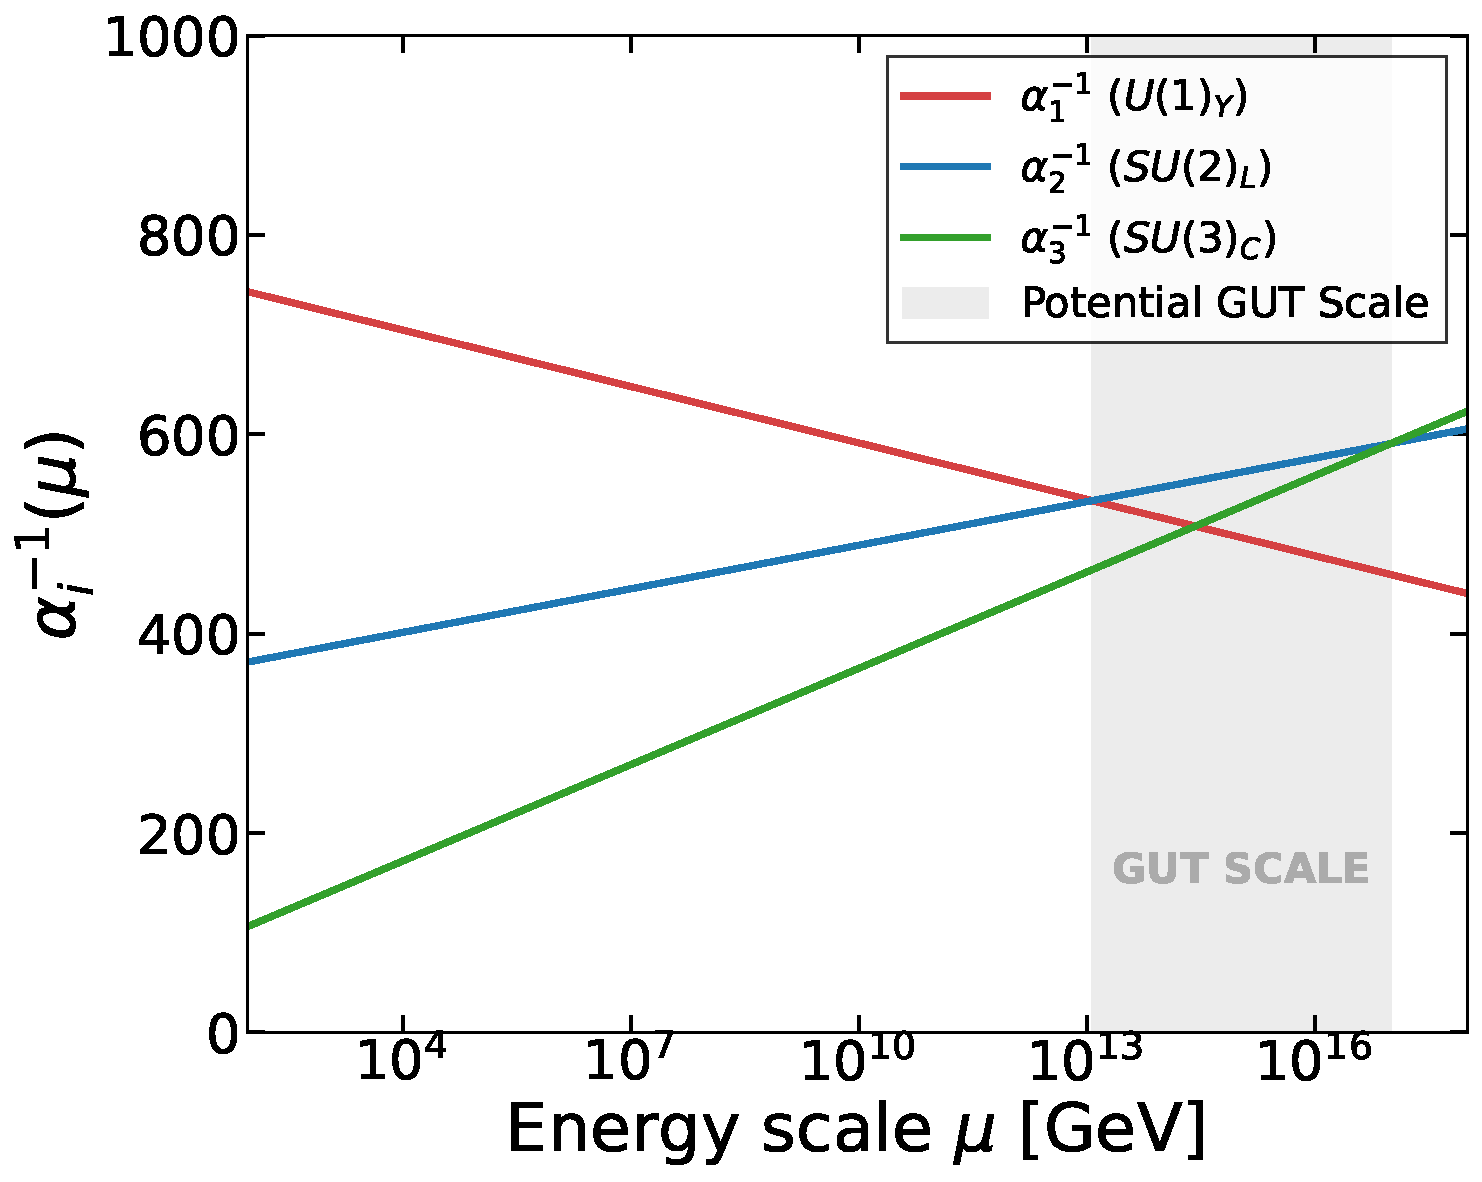
\includegraphics[width=\textwidth]{Figures/sm_unification.pdf}
        \caption{Inverse gauge coupling's dependence on energy scale} % 
        \label{fig:uni}
    \end{subfigure}
    \hspace{0.1cm}
    \begin{subfigure}[b]{0.49\textwidth}
        \centering
        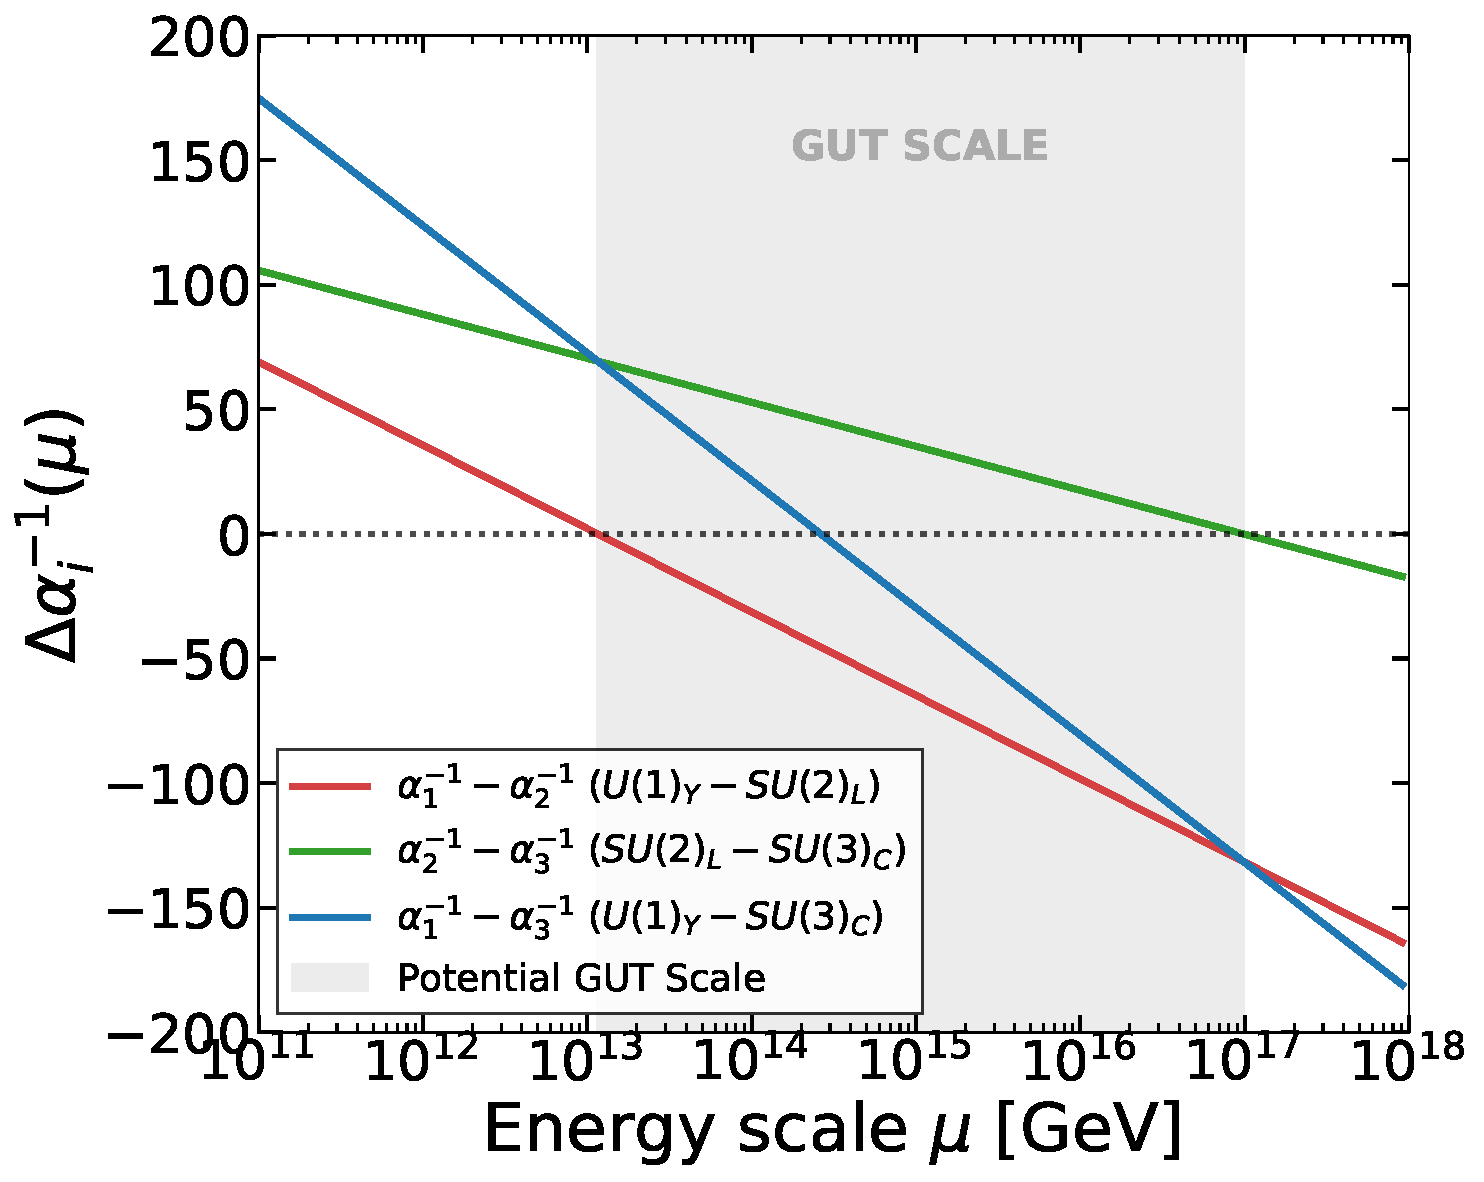
\includegraphics[width=\textwidth]{Figures/sm_unification_differences.pdf}
        \caption{Difference of gauge couplings} 
        \label{fig:uni_diff}
    \end{subfigure}
    \caption{The inverse gauge couplings (Eq. \eqref{eq:RGinversecoupling}) of $\U(1)_Y$ (red), $\SU(2)_L$ (blue), and $\SU(3)_C$ (green) are plotted in (a) against the energy scale in GeV. In (b) the difference of the couplings are shown, where the intersection with zero shows the intersection of (a). }
    \label{fig:SM_unification}
\end{figure}

We define a GUT to be a simple unifying group. However, there are also plenty of examples of product groups as unifying theories. A GUT has two main criteria: It needs to contain the SM gauge sector as a subgroup, and it must have complex representations such that the chiral structure of the SM can be reproduced \cite{Croon:2019kpe}. 

The model we will consider here is the first attempt of unifying the SM, namely the model proposed by H. Georgi and S. Glashow back in 1974 \cite{Georgi:1974yf}. This model is based on the smallest simple group $\SU(5)$, which contains the SM as a subgroup and has complex representations. 

\section{SU(5)}\label{sec:SU5}
\comment{OBS! Make the notation of the particles match the previous section (u,d,e,v vs u,d,Q,L)...}
To consider a possible simple group, which contains the SM gauge sector $\mathrm{SU}(3)_c\times\mathrm{SU}(2)_L\times\mathrm{U}(1)_Y$ as a subgroup, the rank of the group must be at least four, since $\SU(3)_c$ has rank $2$, $\SU(2)_L$ has rank $1$, $\U(1)_Y$ has rank $1$ as well. The simplest group that does this and has complex representations is $\SU(5)$ \cite{Georgi:1999wka}
\begin{equation}
    \mathrm{SU}(3)\times\mathrm{SU}(2)\times\mathrm{U}(1)\subset \mathrm{SU}(5)\,.
\end{equation}
Consider first the particles of the right-handed sector of the SM
\begin{equation}
    u_R^i : (\mathbf{3}, \mathbf{1})_{2/3} \,,\quad 
    d_R^i : (\mathbf{3}, \mathbf{1})_{-1/3} \,,\quad 
    \ell_R^i : (\mathbf{1}, \mathbf{1})_{-1} \,,\quad 
    (Q_L^i)^c : (\bar{\mathbf{3}}, \mathbf{2})_{-1/6} \,,\quad 
    (L_L^i)^c : (\mathbf{1}, \mathbf{2})_{1/2} \,, \label{eq:RparticlesSM}
\end{equation}
where the $c$ indicates the charge conjugated, and $i$ the generation. These particles represent the up quark, down quark, electron, anti-quarks and anti-leptons and can be found in Table \ref{tab:SMparticle}. These representations can be added through a direct sum
\begin{align}
    (3,1)_{2/3}\oplus (3,1)_{-1/3}\oplus (1,1)_{-1}\oplus(\bar{3},2)_{-1/6}\oplus(1,2)_{1/2} \,,
\end{align}
where we can write the complex conjugate of this expression as
\begin{align}
    (\bar{3},1)_{-2/3}\oplus (\bar{3},1)_{1/3}\oplus  (1,1)_{1}\oplus(3,2)_{1/6}\oplus(1,2)_{-1/2} \,.
\end{align}
It has been used that the $\SU(2)_L$ representation is real \cite{Georgi:1999wka}. 

The $\SU(5)$ group has two five-dimensional representations, namely $\bar{\mathbf{5}}$ and $\mathbf{5}$. Thus, we need to determine if the right-handed particles of the SM in Eq. \eqref{eq:RparticlesSM} can be grouped such that they fit in the $\mathbf{5}$ or $\bar{\mathbf{5}}$ multiplet of the $\SU(5)$ group. It is necessary to examine whether the generator of the $\U(1)_Y$ group $Y$ remains traceless\footnote{All the $\SU(N)$ groups are "special" groups, which means that the trace of the generators must be 0. However, the Abelian group $\U(1)_Y$ in the SM is not special and ensuring that the trace of the generator is zero is non-trivial. }. 

To build a $5\times 5$ matrix, we have two options
\begin{align}
    (3,1)_{2/3}\oplus(1,2)_{1/2}\,,\quad\text{or} \quad  (3,1)_{-1/3}\oplus(1,2)_{1/2}\,.\label{eq:irreps5}
\end{align}
To determine whether the combination is valid, we consider the trace of the generator $Y$ for the first option
\begin{align}
    \tr(S)=\tr\begin{pmatrix}
        \frac{2}{3}&0&0&0&0\\
        0&\frac{2}{3}&0&0&0\\
        0&0&\frac{2}{3}&0&0\\
        0&0&0&\frac{1}{2}&0\\
        0&0&0&0&\frac{1}{2}\\
    \end{pmatrix}=3\,.
\end{align}
Since this is not zero, this is not an option. The other case, however, evaluates to zero $(-1/3-1/3-1/3+1/2+1/2=0)$. The $\mathbf{5}$ can now be written as a column vector in terms of the particles of the SM from Eq. \eqref{eq:RparticlesSM}, it will consists of 
\begin{equation}
    \mathbf{5}\leftrightarrow \begin{pmatrix}
        d_1^\dagger\\d_2^\dagger\\d_3^\dagger\\\bar{e} ^\dagger\\\bar{\nu}^\dagger 
    \end{pmatrix}\,. \label{eq:5rep}
\end{equation}
The remaining particles from Eq. \eqref{eq:RparticlesSM} are 
\begin{equation}
     (3,1)_{2/3}\oplus (1,1)_{-1}\oplus(\bar{3},2)_{-1/6} \,,
     \label{eq:5repSU5}
\end{equation}
resulting in a ten-dimensional representation. $\SU(5)$ has two ten-dimensional representations $\overline{\mathbf{10}}$ and $\mathbf{10}$. This can be found by constructing the Young tableau of different direct products of representations of the group (see Appendix \ref{app:youngtab} and \ref{app:youngtabSUN}). We can construct the ten-representation by utilising the product of two fives
\begin{align}
    \mathbf{5} \otimes \mathbf{5} &= \mathbf{15} \oplus \mathbf{10} \,, \\[0.5ex] 
    \vcenter{\hbox{\ydiagram{1}}} \otimes \vcenter{\hbox{\ydiagram{1}}} &= \vcenter{\hbox{\ydiagram{2}}} \oplus \vcenter{\hbox{\ydiagram{1,1}}}\,.
\end{align}
As seen from the computation the symmetric part of the direct product is a $\mathbf{15}$ representation. Thus, we can take the anti-symmetric product of Eq. \eqref{eq:5repSU5} with itself to obtain the $\mathbf{10}$ representation \comment{expand the calulcation like down below}
\begin{align}
    \left[(3,1)_{-1/3}\oplus(1,2)_{1/2}\right]\otimes \left[(3,1)_{-1/3}\oplus(1,2)_{1/2}\right]_{AS}=\left[(\bar{3},1)_{-2/3}\oplus(1,1)_{1}\oplus(3,2)_{1/6}\right]\label{eq:irreps10}
\end{align}
where the hypercharge simply add \cite{Georgi:1999wka}. This gives us the complete conjugate of remaining particles from Eq. \eqref{eq:RparticlesSM}. We can thus write the remaining particles as the $\overline{\mathbf{10}}$ representation.
\begin{align}
\bar{\mathbf{10}} \leftrightarrow 
\begin{pmatrix}
    0 & u_3^\dagger & -u_2^\dagger & \bar{u}^{1\dagger} & \bar{d}^{1\dagger} \\
    -u_3^\dagger & 0 & u_1^\dagger & \bar{u}^{2\dagger} & \bar{d}^{2\dagger} \\
    u_2^\dagger & -u_1^\dagger & 0 & \bar{u}^{3\dagger} & \bar{d}^{3\dagger} \\
    -\bar{u}^{1\dagger} & -\bar{u}^{2\dagger} & -\bar{u}^{3\dagger} & 0 & e^\dagger \\
    -\bar{d}^{1\dagger} & -\bar{d}^{2\dagger} & -\bar{d}^{3\dagger} & -e^\dagger & 0
\end{pmatrix}\,,\label{eq:10barrep}
\end{align}
where $u_a^\dagger$ is right-handed up quarks, $\bar{u}_a^\dagger$ the right-handed anti-up quark, $\bar{d}_a^\dagger$ the right-handed anti-down quark, and $e^\dagger$ is right-handed electrons, where the index $a=1,2,3$ and describes the three colours.   
Note that the anti-symmetric part also ensures that the diagonal entries are trivial and thus that a particle cannot interact with itself. This removes five degrees of freedom from the twenty-five of the $5\times 5$ matrix. Furthermore, the definition of an anti-symmetric matrix also ensures that the entries are mirrored around the diagonal, leaving us with ten degrees of freedom, equal to the ten particles we had yet to describe. Thus, the two representations $\mathbf{5}$ (Eq. \eqref{eq:5rep}) and $\overline{\mathbf{10}}$ (Eq. \eqref{eq:10barrep}) hold all the particles of the SM (seen in Table \ref{tab:SMparticle}).
The same analysis can be done with the left-handed particles, which leaves one with the following representations 
\begin{align}
    \bar{\mathbf{5}}\leftrightarrow \begin{pmatrix}
        \bar{d}_1 \\ \bar{d}_2 \\ \bar{d}_3 \\ e \\ -\nu 
    \end{pmatrix}\quad \mathbf{10}\leftrightarrow \begin{pmatrix}
    0 & \bar{u}_3 & -\bar{u}_2 & u_1 & d_1 \\
    -\bar{u}_3 & 0 & \bar{u}_1 & u_2 & d_2 \\
    \bar{u}_2 & -\bar{u}_1 & 0 & u_3 & d_3 \\
    -u_1 & -u_2 & -u_3 & 0 & \bar{e} \\
    -d_1 & -d_2 & -d_3 & -\bar{e} & 0
\end{pmatrix}
\end{align} 
\subsection{Breaking of the GUT group to the SM gauge groups}
For $\SU(5)$ to be a valid GUT, we need a way of breaking the simple group down to the gauge sector of the SM $\mathrm{SU}(3)\times\mathrm{SU}(2)\times\mathrm{U}(1)$. The $\SU(5)$ group has $N^2-1=24$ gauge bosons, which transforms under the adjoint representation $\mathbf{24}$. The decomposition of this representation into irreducible representations (irreps) (see Appendix \ref{app:repersentations}) SM gauge group can be found by computing
\begin{align}
    \mathbf{5}\otimes\overline{\mathbf{5}}-1_{\SU(5)}\,,
\end{align}
using Eq. \eqref{eq:5rep}, we can write this as 
\begin{align}
    \left[(3,1)_{-1/3}\oplus(1,2)_{1/2}\right]\otimes \left[(\bar{3},1)_{1/3}\oplus(1,2)_{-1/2}\right]-(1,1)_0\,.
\end{align}
To compute this, we use the fact that the hypercharges add. There is only two non-trivial direct products that we have to compute, we will do these explicit. The first one is given by
\begin{align}
    (3,1)_{-1/3}\otimes(\bar{3},1)_{1/3}=(3\otimes\bar{3},1\otimes1)_0=(1,1)_0+(8,1)_0\,,
\end{align}
where
\begin{align}
    (3\otimes{\bar{3}})_{\SU(3)}=\vcenter{\hbox{\ydiagram{1}}} \otimes \vcenter{\hbox{\ydiagram{1,1}}}=\vcenter{\hbox{\ydiagram{1,1,1}}}\oplus \vcenter{\hbox{\ydiagram{2,1}}}\,,
\end{align}
where the $(1,1,1)$ Young tableau is the $\mathbf{1}$ representation, and $(2,1)$ is the $\mathbf{8}$ representation. The other non-trivial term is
\begin{align}
    (1,2)_{1/2}\otimes(1,2)_{-1/2}=(1\otimes1,2\otimes2)_0=(1,1)_0+(1,3)_0\,,
\end{align}
where
\begin{align}
    (2\otimes2)_{\SU(2)}=\vcenter{\hbox{\ydiagram{1}}} \otimes \vcenter{\hbox{\ydiagram{1}}}=\vcenter{\hbox{\ydiagram{1,1}}}\oplus \vcenter{\hbox{\ydiagram{2}}}\,,
\end{align}
where the $(1,1)$ Young tableau is the $1$ representation, and $(2)$ is the $3$ representation. Putting all the terms together, we obtain
\begin{align}
    \mathbf{24}\leftrightarrow (8,1)_0\oplus(1,3)_0\oplus(1,1)_0\oplus (3,2)_{-5/6}\oplus(\bar{3},2)_{5/6}\,. \label{eq:24irrep}
\end{align}
The field content of the adjoint representation of $\SU(5)$ is summarised in Table \ref{tab:adjSU5}. The first three terms in Eq. \eqref{eq:24irrep} is gauge bosons known from the SM (see Table \ref{tab:SMparticle}). The last two terms are however gauge bosons which are not a part of the SM. These force carriers is thus particles, which gain mass at the GUT scale through SSB, and therefore have not been observed experimentally. 
\begin{table}[ht]
\centering
\renewcommand{\arraystretch}{1.4}

\begin{tabularx}{\textwidth}{@{} >{\centering\arraybackslash}X >{\centering\arraybackslash}X >{\centering\arraybackslash}X @{}}
\toprule
\multicolumn{1}{c}{} & \multicolumn{1}{c}{\textbf{Part of the SM}} & \multicolumn{1}{c}{\textbf{Identification}} \\
\midrule
$(8,1)_0$           & \checkmark  & $G_\beta^\alpha$ \\
$(1,3)_0$           & \checkmark  & $W^\pm, W^0$ \\
$(1,1)_0$           & \checkmark  & B \\
$(3,2)_{-5/6}$      & X & $A_\alpha^\tau = (X_\alpha, Y_\alpha)$ \\
$(\bar{3},2)_{5/6}$ & X & $A_\tau^\alpha = (X_\alpha, Y_\alpha)^T$ \\
\bottomrule
\end{tabularx}
\caption{Gauge boson of the $\SU(5)$ GUT from the $24$ representation (Eq. \eqref{eq:24irrep}) and their identifications.}
\label{tab:adjSU5}
\end{table}

We can understand the SSB by writing the adjoint representation as a matrix using the generator $t^a$ 
\begin{align}
    \Phi=\phi^at^a\,,
\end{align}
where $a=1,2,\dots,24$ is the adjoint index \cite{Pernow:2021fvb}. Thus, the adjoint representation can be expressed as
\begin{equation}
    \Phi=\begin{pmatrix}
        A_{3\times3}&B_{3\times 2}\\
        C_{2\times3}&D_{2\times 2}
    \end{pmatrix}\,,
\end{equation}
where the subscript refers to the dimension of the submatrix. The upper left submatrix $A_{3\times3}$ acts like the strong force, $D_{2\times2}$ is equivalent to the weak force, and $B_{3\times2}$ and $C_{2\times3}$ mixes the strong and the weak force and are generally called the $X$ and $Y$ bosons, these are the ones which will eat the Goldstone bosons and require mass \cite{Peskin:1995ev}. 

The breaking of the $\SU(5)$ group is done analogously to the Higgs mechanism of the SM \cite{Pernow:2021fvb}. A scalar field transforming in the adjoint representation of the gauge group acquires a VEV. In this breaking we do not wish to break down the gauge structure of the SM. Thus the VEV needs to commute with the generators of $\mathcal{G}_{\mathrm{SM}}$. It is therefore useful to take a VEV which is proportional to the traceless $Y$ generator \cite{Georgi:1999wka}.    

To understand the SSB of $\SU(5)$, we consider the general renormalisable potential for the adjoint scalar
\begin{align}
    V=-\mu_1^3\tr\Phi-\mu_2^2\tr\Phi^2-\mu_3\tr\Phi^3+\lambda_1(\tr\Phi^2)^2+\lambda_2\tr\Phi^4\,,
\end{align}
where we can simplify the potential using that the generators $t^a$ of $\SU(N)$ are traceless and that we can impose parity symmetry. This yields
\begin{align}
    V=-\mu^2\tr\Phi^2+\lambda_1(\tr\Phi^2)^2+\lambda_2\tr\Phi^4\,.\label{eq:SU5pot}
\end{align}

We can now find a VEV of the potential. However, we must ensure that it commutes with the $Y$ generator. For convenience we consider $(-6)$ times the hypercharge
\begin{align}
    \langle\Phi\rangle=v\,\mathrm{diag}(2,2,2,-3,-3)\,.\label{eq:VEVdiag}
\end{align}
Before specifying the value of $v$, we first need to constrain our values of $\lambda_1,\,\lambda_2$ by considering all possible breaking of $\SU(5)$ \comment{check Peskin exercise}
\begin{align*}
    &\begin{pmatrix} a & & & & \\ & a & & & \\ & & a & & \\ & & & b & \\ & & & & b \end{pmatrix} \to \begin{matrix} 3a + 2b = 0 \\ \SU(3) \times \SU(2) \end{matrix} 
    & \begin{pmatrix} a & & & & \\ & b & & & \\ & & c & & \\ & & & d & \\ & & & & e \end{pmatrix} \to \begin{matrix} a+b+c+d+e = 0 \\ \U(1)\times \U(1)\times\U(1)\times\U(1)\times\U(1) \end{matrix} \\[15pt]
    &\begin{pmatrix} a & & & & \\ & a & & & \\ & & a & & \\ & & & a & \\ & & & & b \end{pmatrix} \to \begin{matrix} 4a + b = 0 \\ SU(4) \times U(1) \end{matrix} 
    &\begin{pmatrix} a & & & & \\ & a & & & \\ & & a & & \\ & & & b & \\ & & & & c \end{pmatrix} \to \begin{matrix} 3a + b + c = 0 \\ SU(3) \times U(1) \times U(1) \end{matrix} \\[15pt]
    &\begin{pmatrix} a & & & & \\ & a & & & \\ & & b & & \\ & & & b & \\ & & & & c \end{pmatrix} \to \begin{matrix} 2(a + b) + c = 0 \\ SU(2) \times SU(2) \times U(1) \end{matrix} 
    &\begin{pmatrix} a & & & & \\ & a & & & \\ & & b & & \\ & & & c & \\ & & & & d \end{pmatrix} \to \begin{matrix} 2a + b + c + d = 0 \\ SU(2) \times U(1) \times U(1) \times U(1) \end{matrix}
\end{align*}
As already noted, the desired breaking is the first which successfully breaks $\SU(5)$ to the SM. To ensure this is the VEV the model actually realises, we need to ensure that it is the minimal VEV. In general, when theories break down to more complex group structures, the VEV becomes larger. We can thus focus on the two simplest sets of eigenvalues, where there are only two variables. First, we can write the derivative of the potential (Eq. \eqref{eq:SU5pot}) in a general form
\begin{align}
    \frac{\partial V}{\partial v}=-2\mu^2 v A+4v^3(\lambda_1A^2+\lambda_2B)\,,
\end{align}
where $A=\tr\Phi^2/v^2$ and $B=\tr\Phi^4/v^4$. If we now minimise the potential, the expression for $v^2$ yields
\begin{align}
    v^2=\frac{\mu^2 A}{2(\lambda_1A^2+\lambda_2B)} \label{eq:VEVvalue}
\end{align}
Let us plug this back into the potential Eq. \eqref{eq:SU5pot} and simplify 
\begin{align}
    V_{\min}&=-\mu^2A\frac{\mu^2 A}{2(\lambda_1A^2+\lambda_2B)}+\lambda_1A^2\left(\frac{\mu^2 A}{2(\lambda_1A^2+\lambda_2B)}\right)^2+\lambda_2B\left(\frac{\mu^2 A}{2(\lambda_1A^2+\lambda_2B)}\right)^2\nonumber
    \\
    &=-\frac{\mu^4 A^2}{2(\lambda_1A^2+\lambda_2B)}+\lambda_1\frac{\mu^4 A^4}{4(\lambda_1A^2+\lambda_2B)^2}+\lambda_2\frac{\mu^4 A^2B}{4(\lambda_1A^2+\lambda_2B)^2}\nonumber
    \\
    &=\frac{-2(\lambda_1A^2+\lambda_2B)\mu^4 A^2+\mu^4 A^4\lambda_1+\mu^4 A^2B\lambda_2}{4(\lambda_1A^2+\lambda_2B)^2}\nonumber
     \\
    &=\frac{-\mu^4A^2}{4(\lambda_1A^2+\lambda_2B)^2}\left[2(\lambda_1A^2+\lambda_2B)-A^2\lambda_1-B\lambda_2\right]\nonumber
    \\
    &=\frac{-\mu^4A^2}{4(\lambda_1A^2+\lambda_2B)}
\end{align}
Thus the minimal potential depends on $\lambda_{\text{eff}}$ as
\begin{align}
    V_{{\min}}\sim-\frac{\mu^4}{\lambda_{\text{eff}}}\,,\label{eq:1/lambdaeff}
\end{align}
where $\lambda_{\text{eff}}=\lambda_1+\lambda_2\frac{B}{A^2}$. 

To ensure that we obtain the $\SU(3) \times \SU(2)$ breaking rather than the $\SU(4) \times \U(1)$ breaking, we can compute the values of $A$ and $B$ in both cases. For the first case 
\begin{align}
    A_{(3,2)} &= \frac{\tr(\Phi^2)}{v^2} = 3a^2 + 2\left(-\frac{3}{2}a\right)^2 = \frac{15}{2} a^2 \,, \label{eq:VEVA_32} \\
    B_{(3,2)} &= \frac{\tr(\Phi^4)}{v^4} = 3a^4 + 2\left(-\frac{3}{2}a\right)^4 = \frac{105}{8} a^4 \,. \label{eq:VEVB_32}
\end{align}
where the condition $b=-\frac{3}{2}a$ has been used. In the second case, we obtain 
\begin{align}
    A_{(4,1)} &=  4a^2 + (-4a)^2 = 20a^2 \,, \label{eq:VEVA_41} \\
    B_{(4,1)} &= 4a^4 + (-4a)^4 = 260a^4 \,. \label{eq:VEVB_41}
\end{align}
where $b=-4a$ has been used. To ensure that the VEV is smaller in the case of $\SU(3) \times \SU(2)$ breaking, a boundary on the quartic coupling, using Eq. \eqref{eq:1/lambdaeff}, is obtained
\begin{align}
    V_{(3,2)}&<V_{(4,1)}\\
    \lambda_{\text{eff}_{(3,2)}}&<\lambda_{\text{eff}_{(4,1)}}
    \\\lambda_2 \frac{7}{30}&<\lambda_2\frac{13}{20}\,.
\end{align}
This is only the case for $\lambda_2>0$. 

Now to ensure a bounded potential from below, we also require $\lambda_{\text{eff}}>0$. From this, we obtain a boundary on $\lambda_1$
\begin{align}
    \lambda_{\text{eff}}&>0\\
    \lambda_1&>-\lambda_2\frac{7}{30}\,.
\end{align}
This effectively breaks down our gauge group from $\SU(5)\to\SU(3)\times\SU(2)\times\U(1)$, since $\U(1)_Y$ by construction commutes with the VEV. This ensures that the X and Y bosons gain mass at the GUT scale. After symmetry-breaking, eight of the twenty-four gauge bosons are the gluons, three are the weak gauge bosons, and one is the hypercharge gauge boson \cite{Pernow:2021fvb} as seen in Table \ref{tab:adjSU5}.

With the constraints on $\lambda_2$ and $\lambda_1$, the VEV can be found by combining Eqs. \eqref{eq:VEVvalue} and \eqref{eq:VEVdiag}
\begin{align}
    \langle \Phi\rangle=\frac{\mu^2}{2(30\lambda_1+7\lambda_2)}\mathrm{diag}(2,2,2,-3,-3)\,,
\end{align}
where the values of $A$ and $B$ are given by Eqs. \eqref{eq:VEVA_32} and \eqref{eq:VEVB_32}.

\subsection{The Higgs boson in SU(5)}
With the GUT broken down to the SM, the next step is to introduce a scalar field which can break the electroweak symmetry, playing the role of the Higgs boson in the SM. The Higgs transforms as $(1,2)_{\pm1/2}$ under $\mathcal{G}_\mathrm{SM}$. This scalar is required to  generate mass for the right-handed positron $(\bar{e})$ and the down type quarks $(d)$.  These specific states reside in the $\mathbf{5}$ representation (see Eq. \eqref{eq:5repSU5}), and their corresponding anti-particles in $\overline{\mathbf{10}}$ (see Eq. \eqref{eq:10barrep}). Their mass term must arise from the tensor product of these representations \cite{Georgi:1999wka}
\begin{align}
     (\overline{\mathbf{10}}\otimes{\mathbf{5}})_{\SU(5)}=\vcenter{\hbox{\ydiagram{1,1,1}}} \otimes \vcenter{\hbox{\ydiagram{1}}}=\vcenter{\hbox{\ydiagram{2,1,1}}}\oplus \vcenter{\hbox{\ydiagram{1,1,1,1}}} =\overline{\mathbf{45}}\otimes \overline{\mathbf{5}}\,, 
\end{align} 
Besides from the positron and down type quarks, the scalar must also generate masses for the ${u}$ and $\overline{u}$ states, both of which is contained in the $\overline{\mathbf{10}}$ representation. Let us consider the product of the representation with itself
\begin{align}
     (\overline{\mathbf{10}}\otimes{\overline{\mathbf{10}}})_{\SU(5)}&=\vcenter{\hbox{\ydiagram{1,1,1}}} \otimes \vcenter{\hbox{\ydiagram{1,1,1}}}\\&\implies
\begin{ytableau} ~ \\ ~ \\ ~ \end{ytableau} \otimes \begin{ytableau} a \\ b \\ c \end{ytableau} 
= \left(
\begin{ytableau} ~ \\ ~ \\ ~ \\ a \end{ytableau} \oplus 
\begin{ytableau} ~ & a \\ ~ \\ ~ \end{ytableau}
\right) \otimes \begin{ytableau} b \\ c \end{ytableau} 
= \left(
\begin{ytableau} ~ \\ ~ \\ ~ \\ a \\ b \end{ytableau} \oplus 
\begin{ytableau} ~ & a \\ ~ & b \\ ~ \end{ytableau} \oplus 
\begin{ytableau} ~ & a \\ ~ \\ ~ \\ b \end{ytableau}
\right) \otimes \begin{ytableau} c \end{ytableau} \\
&= \begin{ytableau} ~ \\ ~ \\ ~ \\ a \\ b \\ c \end{ytableau} \oplus 
\begin{ytableau} ~ & a \\ ~ & b \\ ~ \\ c \end{ytableau} \oplus 
\begin{ytableau} ~ & a \\ ~ & b \\ ~ & c \end{ytableau}=\begin{ytableau} ~ \\ \end{ytableau} \oplus 
\begin{ytableau} ~ & ~ \\ ~ & ~ \\ ~ \\ ~ \end{ytableau} \oplus 
\begin{ytableau} ~ & ~ \\ ~ & ~ \\ ~ & ~ \end{ytableau}={\mathbf{5}}\oplus {\mathbf{45}}\oplus {\mathbf{50}}
\end{align}
To determine the allowed representations, the decomposition of the representations need to contain a multiplet with the same quantum numbers of the SM Higgs $(1,2)_{\pm1/2}$. The Higgs like scalar can reside in either the ${\mathbf{5}}$ or ${\mathbf{45}}$ \cite{Georgi:1999wka} (see Eq. \eqref{eq:irreps5} for the ${\mathbf{5}}$ representation). To confirm that this is also the case for the ${\mathbf{45}}$ representation we can compute the direct product of the two representations ${\mathbf{5}}\otimes\overline{{\mathbf{10}}}$. We will demonstrate this by utilising the decomposition in Eq. \eqref{eq:irreps5} and \eqref{eq:irreps10}, which yields
 \begin{align}
    &\left( (3,1)_{-1/3} \oplus (1,2)_{1/2} \right) \otimes \left( (3,1)_{2/3} \oplus (1,1)_{-1} \oplus (\bar{3},2)_{-1/6} \right) \\&= (6,1)_{1/3} \oplus (\bar{3},1)_{1/3} \oplus (3,1)_{-4/3} \oplus (\bar{8},2)_{-1/2} \oplus (1,2)_{-1/2} \nonumber\\&\quad\oplus (3,2)_{7/6} \oplus (1,2)_{-1/2}\oplus (\bar{3},3)_{1/3}\oplus (\bar{3},1)_{1/3}\,.
\end{align}
We can now remove the irreps which make out the $\mathbf{5}$ representations (see Eq. \eqref{eq:irreps5}), effectively revealing the decomposition of the $\mathbf{45}$ representation
 \begin{align}
    \mathbf{45}\leftrightarrow&\left( (3,1)_{-1/3} \oplus (1,2)_{1/2} \right) \otimes \left( (3,1)_{2/3} \oplus (1,1)_{-1} \oplus (\bar{3},2)_{-1/6} \right) \\&= (6,1)_{1/3} \oplus (\bar{3},1)_{1/3} \oplus (3,1)_{-4/3} \oplus (\bar{8},2)_{-1/2} \oplus (1,2)_{-1/2} \oplus (3,2)_{7/6} \oplus (\bar{3},3)_{1/3}\,,
\end{align}
which includes the Higgs like irrep $(1,2)_{-1/2} $. Thus both ${\mathbf{5}}$ or ${\mathbf{45}}$ can be used to introduce a Higgs like scalar into the GUT.  

While conceptually compelling, the minimal $\SU(5)$ model encounters fundamental issues. A theoretical limitation of the model is the so-called \textit{doublet-triplet splitting} \cite{Croon:2019kpe}. This issue arises from the embedding the Higgs scalar within the $\mathbf{5}$ representation. This choice requires fine-tuning of the masses of the multiplets coloured components compared to the uncoloured components. The colour-triplet states needs to be heavy (around GUT scale) to avoid proton decay with a low decay rate. In contrast to the uncoloured doublet needs to be relatively light to ensure that the Higgs mass is in agreement with the measured mass of the Higgs $m_H=125.18\,$GeV \cite{Croon:2019kpe}. 

A further shortcoming of the model is its lack of generating neutrino mass. Different attempts to fix this have been proposed see \cite{FileviezPerez:2007bcw, Zee:1980ai,FileviezPerez:2016sal}. 

Lastly, the biggest challenge of the model is its prediction of rapid proton decay. The mixing of quarks and leptons in the representations successfully explains the neutralness of the atom. However, this mixing also results the $X$ and $Y$ gauge bosons, which mediate the proton decay and estimates the proton lifetime at \cite{Croon:2019kpe}
\begin{align}
    \tau_p\sim\frac{M_X^4}{m_p^5}\,,
\end{align}
where $m_p$ is the mass of the proton and $M_X$ is the scale of unification. As seen in Figures \ref{fig:uni} above, the assumed unification scale is around $\mu\sim10^{15}\,$GeV. This results in a proton decay rate of $\sim10^{31}\,$years. Since proton decay has not (yet) been observed, there is an experimental lower bound on the decay time of proton at the order of $10^{34}\,$years \cite{Takenaka:2020cmb}. This bound is the results of the experiment the Super-Kamiokande and is thus in disagreement with the estimate from the $\SU(5)$ GUT. Changes to the Higgs sector of the model can help this problem, see \cite{Dorsner:2005fq,Dorsner:2006dj,Fornal:2017xcj,FileviezPerez:2018dyf}. 

\section{Alternative GUTs}
The unification of the SM gauge groups does not necessarily need to be restricted to be the simplest embedding. Investigating larger symmetry groups provides alternative frameworks, with on of them being the $\mathrm{SO}(10)$ group. This group has the $\SU(5)$ GUT as a subgroup \cite{Georgi:1999wka}
\begin{equation}
    \mathrm{SU}(5)\times \U (1)\subset \mathrm{SO}(10)\,.
\end{equation}
The $\SO (10)$ GUT also suffer from the prediction of proton decay, however it resolves several of $\SU(5)$'s issues. Most notably, the $\SO(10)$ generates neutrino masses, through the inclusion of a right-handed neutrino. Furthermore, it fits the entire particle content of the SM into one single $\mathbf{16}$ representation \cite{Fritzsch:1974nn}. 

Besides the $\SU (5)$ and $\SO(10)$ GUTs, there are multiple other possibilities, such as the exceptional Lie group \cite{Gursey:1975ki}
\begin{equation}
    \SU(5)\subset\SO(10)\subset\E_6\,.
\end{equation}
This embedding of the SM is particularly studied within the string theory community, because the group structure of $\E_6$ is a subgroup of $\E_8\times\E_8$, which is the group structure of \textit{heterotic string theory} \cite{Witten:1985xc,Candelas:1985en}. This would essentially introduce a possible theory of everything, which would break down to an $\E_6$ GUT. This model, however, suffers from a large fundamental representation of $\mathbf{27}$, which introduces a lot of new particles, besides the particles from the SM. Furthermore, the Higgs sector is based on large representations and the breaking of the model down to the SM introduces an extra gauge boson, which has not been discovered experimentally \cite{Langacker:2008yv}. 

Another set of models are semi-simple groups, such as Pati--Salam \cite{Pati:1974yy} $\SU(4)_C\times \SU(2)_L\times\SU(2)_R$. This GUT restores the left-right symmetry at high energies and at low energies, the $\SU(2)_R$ is broken, ensuring the left-handed bias that we have in the SM. Additionally, it gauges the lepton number as a symmetry. 

Another semi-simple GUT is the so-called Flipped $\SU(5)$ \cite{Barr:1981qv,DeRujula:1980qc} which has the gauge structure $\SU(5)\times\U(1)$. This model solves the doublet-triplet splitting problem of the minimal $\SU(5)$ discussed above \cite{Croon:2019kpe}. 

Other models such as Trinification $\SU(3)\times\SU(3)\times\SU(3)$ has also been explored \cite{Achiman:1978rv}.

Despite the models individual shortcomings and differing particle additions, all GUTs share the same core requirements. They must include the necessary fermion generations, supply the scalar fields required to break the unified group down to the SM, and a scalar to play the role of the Higgs.

Another possibility is supersymmetric (SUSY) GUTs \cite{Dimopoulos:1981zb}. This introduces a symmetry between bosons and fermions, resulting in twice the number of particles in the SM. Every particle would have a supersymmetric counterpart; for instance: quarks would have \textit{squarks}, and leptons would have \textit{sleptons}. One of the models shortcomings is that none of the supersymmetric particles has been found yet. A quality of the SUSY GUT is that the Figure \ref{fig:uni} will change, and have an actual intersection of all three couplings at the SUSY GUT scale $10^{16}\,$GeV. This ensures a higher decay time for protons and thus the $\SU(5)$ GUT would not be ruled out based on the prediction of proton decay. 

In this thesis, we will focus on simple GUTs based on non-SUSY $\SU(N)$ groups. In the next chapter, we will explore \textit{complete asymptotic freedom} of the $\SU(N)$ groups.  


\chapter{CAF Framework}
\label{chap:CAF}
When constructing viable GUTs, it is necessary to ensure that the model remains consistent at small distances. One possible approach to this is to ensure that all the couplings are asymptotically free at high energies, this leads us to the framework of \textit{complete asymptotic freedom} (CAF) \cite{Giudice:2014tma, Pica:2016krb}. CAF requires that the Yukawa and quartic couplings vanish faster than or at the same rate as the gauge coupling, which has to be asymptotically free. 

The analysis within this framework can be split into two primary approaches. The first involves solving the system of coupled beta functions analytically to evaluate the evolution of the coupling with the energy scale. This approach will be considered in the first Section \ref{sec:CAFODE} in this chapter.

The second approach is a polynomial method, which is useful when dealing with multiple couplings of various types. By assuming \textit{fixed flow}, the beta functions can be transformed from coupled ODEs into coupled algebraic equations. Depending on the polynomial order, these can be solved numerically or analytically, as explained in Section \ref{sec:CAF2}. 

\section{ODE approach}\label{sec:CAFODE}
To constrain the coefficients of the RG equations of a gauge-Yukawa theory with scalars, we will start by considering a pure gauge theory and work our way to the full model, following a similar approach to \cite{Giudice:2014tma, Pica:2016krb}. The introduction of scalars are necessary to realise a physical GUT as reviewed in Section \ref{sec:SU5}. As we seek to find vanishing values of the couplings, we only consider one-loop beta functions. 
\subsection{Gauge Coupling}\label{sec:CAFgauge}
Consider first the gauge coupling's beta function $\beta_g$ to one-loop order (defined in Eq. \eqref{eq:betafunc})
\begin{equation}
    \beta_g:=\mu\frac{\text{d}\alpha_g}{\text{d}\mu}\implies \beta _g= b_0\alpha_g^2\,,\label{eq:betag1loopcaf}
\end{equation}
where $\mu$ is the RG scale, $\alpha_g=\frac{g^2}{(4\pi)^2}$. The coefficient $b_0$ is given in Eq.~\eqref{eq:b0def} for a non-Abelian gauge group. We will consider $b_0$ a constant in the CAF analysis below. For the pure gauge theory to be asymptotically free \cite{Politzer:1974fr}, the beta function must be negative, i.e.\ with our definition\footnote{Note that some authors define $\beta_g:=-b_0\alpha_g^2$, which changes the overall sign in the subsequent analysis.} in Eq.~\eqref{eq:betag1loopcaf}, $b_0<0$. 
The solution of the differential equation is
\begin{equation}
    \alpha_g=\frac{\alpha_{g_0}}{1-b_0 \alpha_{g_0} \ln \left(\frac{\mu}{\mu_0 }\right)}\,,
    \label{eq:solbetag1loop}
\end{equation}
where the initial condition is $\alpha(\mu_0)=\alpha_{g_0}$, with $\mu_0$ as the reference RG scale. 

In the case where $\mu<\mu_L$, with $\mu_L=\mu_0\exp(1/{b_0\alpha_{g_0}})$, the denominator is negative since $b_0<0$, resulting in a negative coupling, which will be a non-physical branch. In the case where $\mu=\mu_L$, we have a Landau pole in the infrared (IR). Finally, when $\mu>\mu_L$, the coupling is positive and will vanish as $\mu\to\infty$ signifying asymptotic freedom.
\subsection{Yukawa Coupling }\label{sec:CAFYukawa}
An analogous analysis can be carried out using the RG equations governing the Yukawa couplings, which depend on the gauge coupling at one loop. For simplicity, we will consider a single Yukawa coupling $\alpha_y$ with the following beta function
\begin{equation}
    \beta_y:=\mu \frac{\text{d}\alpha_y}{\text{d}\mu}=\alpha_y(c_1\alpha_g+c_2\alpha_y)\,,\label{eq:betay1loop}
\end{equation}
where $\alpha_y=\frac{y^2}{(4\pi)^2}$, and $c_1$, $c_2$ are constants, where in general $c_1<0$ and $c_2>0$. First, let us consider the case of a vanishing gauge coupling, i.e.\ $\alpha_g=0$. In this case, the solution is analogous to that of the pure gauge theory (see Eq.~\eqref{eq:solbetag1loop}), 
\begin{equation}
    \alpha_y=\frac{\alpha_{y_0}}{1-c_2 \alpha_{y_0} \ln \left(\frac{\mu}{\mu_0 }\right)}\,,
\end{equation}
with the crucial difference being that the constant $c_2$ is positive. Therefore, in the high energy limit $\mu\to\infty$ the denominator becomes negative, resulting in a non-physical branch. For $\mu<\mu_L$ with $\mu_L=\mu_0\exp(1/{c_2\alpha_{y_0}})$ the coupling is positive. Thus, the coupling flows to the Gaussian fixed point in the IR and flows towards a Landau pole in the UV. This establishes that the Yukawa coupling can never be asymptotically free in the absence of a gauge coupling. Thus, when the gauge coupling flows to zero in the UV, so must the Yukawa coupling as fast as $\alpha_g$ or faster, to ensure that the contribution of the gauge coupling to the Yukawa beta function (Eq.~\eqref{eq:betay1loop}) remains sizeable. 

Let us turn to the case of $\alpha_g\neq0$. We now have a system of two coupled differential equations. A solution can be found utilising the ratio method \cite{Pendleton:1980as} on the Yukawa (Eq.~\eqref{eq:betay1loop}) and gauge (Eq.~\eqref{eq:betag1loopcaf}) beta functions 
\begin{align}
    \frac{\beta_y}{\beta_g}=\frac{\text{d}\alpha_y}{\text{d}\alpha_g}&= \frac{\alpha_y(c_1 \alpha_g + c_2 \alpha_y)}{b_0 \alpha_g^2} = \frac{\alpha_y}{b_0 \alpha_g} \left( c_1 + c_2 \frac{\alpha_y}{\alpha_g} \right)\,.\label{eq:betayfrac}
\end{align}
The solutions to the differential equation depend on $b_0$ and $c_1$. 

\paragraph{Case 1 $b_0=c_1$:} In this case the solution is given by 
\begin{equation}
    \alpha_y=\frac{\alpha_{y_0}}{\alpha_{g_0}\left(1+\frac{c_2}{c_1}\frac{\alpha_{y_0}}{\alpha_{g_0}}\ln\alpha_{g_0}\right)-\frac{c_2}{c_1}\alpha_{y_0}\ln \alpha_g }\alpha_g\,,\label{eq:ysolb0c1}
\end{equation}
with the initial condition $\alpha_y(\alpha_{g_0})=\alpha_{y_{0}}$. As $\alpha_g\to0$ the denominator will be dominated by the second term  $(-\frac{c_2}{c_1}\alpha_{y_0}\ln \alpha_g) $, since the logarithm of the gauge coupling will go towards negative infinity. Because the constant in front will always be negative $\frac{c_2}{c_1}<0$, the $\alpha_y$ coupling will be negative. Thus, we have no CAF solution in this case, since the Yukawa coupling follows a non-physical branch as the gauge coupling goes to zero, and we approach the UV. 

\paragraph{Case 2 $b_0\neq c_1$:} The solution changes to
\begin{equation}
    \alpha_y=\frac{\alpha_{y_0}}{ \alpha_g^{1-\frac{c_1}{b_0}}\alpha_{g_0}^{\frac{c_1}{b_0}}\left(1-\frac{c_2}{b_0-c_1}\frac{\alpha_{y_0}}{\alpha_{g_0}}\right)+\frac{c_2}{b_0-c_1}\alpha_{y_0} }\alpha_g\,.\label{eq:sol2g}
\end{equation}
The equation can be divided into two parts, one which will be dependent on $\alpha^{\frac{c_1}{b_0}}_g$ and one on $\alpha_g$. If $\frac{c_1}{b_0}>1$, the first term will dominate and for $\frac{c_1}{b_0}<1$ the second term will dominate. The case of $\frac{c_1}{b_0}=1$ has already been ruled out by the analysis of Eq.~\eqref{eq:ysolb0c1}. In the case of $\frac{c_1}{b_0}<1$, the coupling will go as 
\begin{equation}
    \alpha_y\sim\frac{b_0-c_1}{c_2}\alpha_g\,,\quad\quad 0>{c_1}>b_0\,,
\end{equation}
which is always negative, since $b_0-c_1<0$. Therefore, this scenario does not yield an asymptotically free Yukawa coupling. 

The final possibility is the regime where $\frac{c_1}{b_0}>1$. Here, the coupling behaves as
\begin{equation}
    \alpha_y\sim\frac{\alpha_{y_0}}{ \alpha_{g_0}^{\frac{c_1}{b_0}}\left(1-\frac{c_2}{b_0-c_1}\frac{\alpha_{y_0}}{\alpha_{g_0}}\right)}\alpha_g^{\frac{c_1}{b_0}}\,,\quad\quad \frac{\alpha_{g_0}}{\alpha_{y_0}}>\frac{c_2}{b_0-c_1}\,,\quad\quad c_1<b_0<0\,.\label{eq:Yukawacondoff}
\end{equation}
To ensure that the coupling will be positive, we need to constrain the values of the couplings at the RG reference scale: $\frac{c_2}{b_0-c_1}\frac{\alpha_{y_0}}{\alpha_{g_0}}<1$. In the UV, where $\alpha_g\to 0$, the Yukawa coupling will also be asymptotically free, and because $\frac{c_1}{b_0}>1$, the Yukawa coupling will go faster to zero than the gauge coupling at high energies. 

Another possibility is that the values of the couplings at the arbitrary energy level are fine-tuned $\frac{\alpha_{g_0}}{\alpha_{y_0}}=\frac{c_2}{b_0-c_1}$. In this case, the first term in the denominator in Eq.~\eqref{eq:sol2g} vanishes, and the previously dominated term is now the only one left:
\begin{equation}
    \alpha_y=\frac{b_0-c_1}{ c_2 }\alpha_g\,,\quad\quad \frac{\alpha_{g_0}}{\alpha_{y_0}}=\frac{c_2}{b_0-c_1}\,,\quad\quad b_0-c_1>0\,.\label{eq:ygfixed}
\end{equation}
This case is known as fixed flow \cite{Giudice:2014tma}. Along this trajectory, the Yukawa coupling vanishes with the same rate as the gauge coupling, i.e.\ the ratio $\alpha_y/\alpha_g$ flows to a constant. 

Thus, there are two ways to obtain a CAF regime for a system with a single gauge and Yukawa coupling: the couplings must follow either a fixed-flow trajectory (Eq.~\eqref{eq:ygfixed}) or an off-fixed-flow trajectory (Eq.~\eqref{eq:Yukawacondoff}). This distinction is illustrated by the RG flow plot in Figure~\ref{fig:gYCAFplot}. The values of the coefficients $b_0$ and $c_1$ are chosen such that they satisfy the CAF conditions (see Eq.~\ref{eq:Yukawacondoff}). The couplings exhibit fixed-flow behaviour only along the green trajectory. In this scenario, the values of the gauge and Yukawa couplings at the reference RG scale are more tightly constrained than in the off-fixed-flow regime, which corresponds to the region below the green line. Finally, trajectories above the green line do not exhibit CAF. This demonstrates the requirements on $\alpha_{g_0}$ as well as $\alpha_{y_0}$ to realise a CAF region, in addition to the constraints on the coefficients of the beta function (see Eq.~\eqref{eq:ygfixed}). 

\begin{figure}[h!]
    \centering
    \begin{subfigure}[b]{0.48\textwidth}
        \centering
        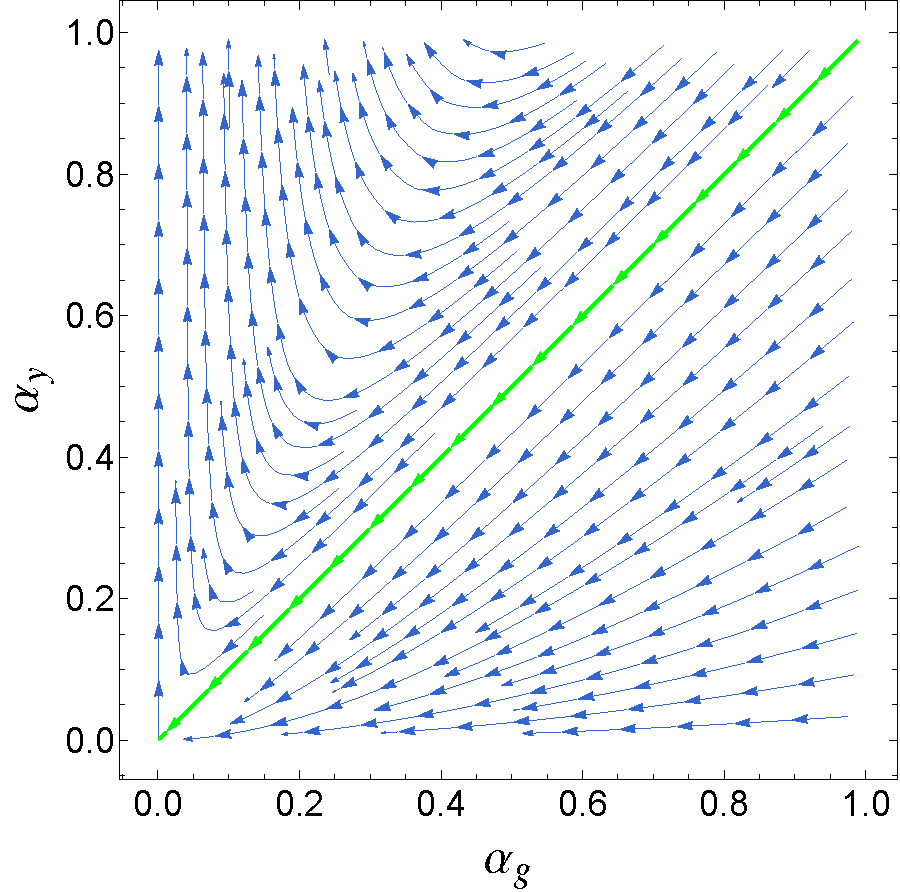
\includegraphics[width=\textwidth]{Figures/Flowplottest2.pdf}
        \caption{$(\alpha_g,\alpha_y)$} 
        \label{fig:gYCAFplot}
    \end{subfigure}%
    \hfill
    \begin{subfigure}[b]{0.48\textwidth}
        \centering
        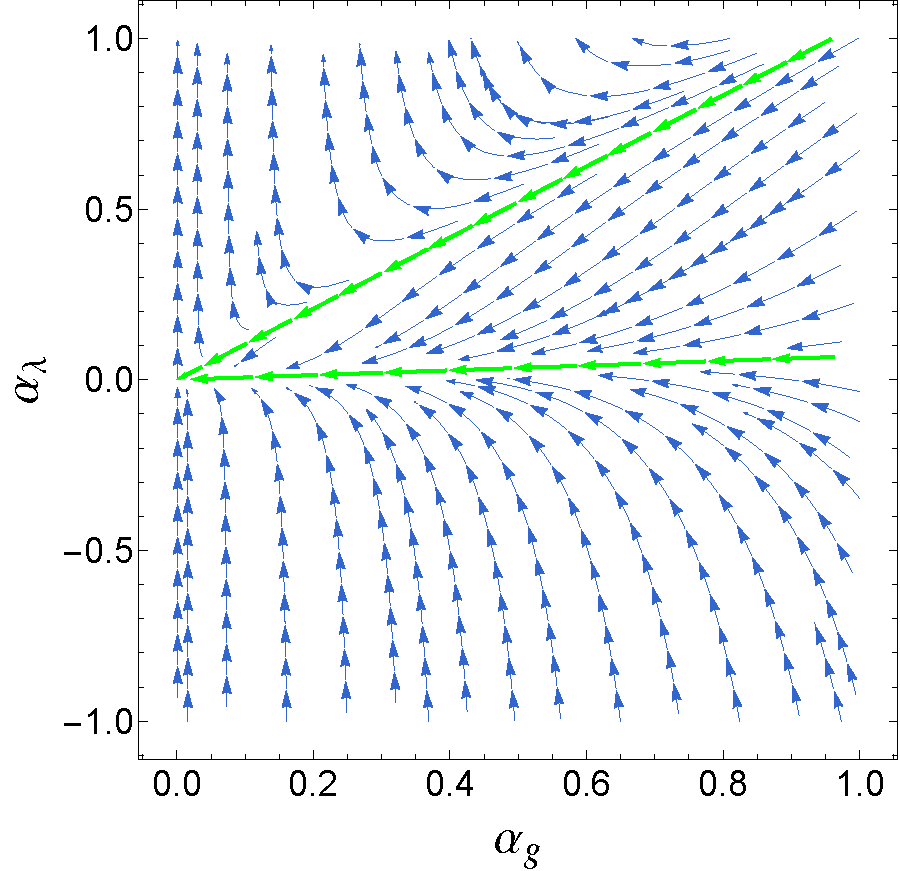
\includegraphics[width=\textwidth]{Figures/Scalarflow.pdf}
        \caption{$(\alpha_g,\alpha_\lambda)$}
        \label{fig:glamCAFplot}
    \end{subfigure}
    \caption{The RG flow of a CAF solution for all three couplings when the Yukawa coupling is off-fixed flow, thus upholding Eq.~\eqref{eq:CAF}. Panel (A) is in the $(\alpha_g,\alpha_y)$ parameter space and panel (B) is in the $(\alpha_g,\alpha_\lambda)$ parameter space. The green flow lines illustrate the fixed-flow of the couplings in the respective coupling space. All arrows point towards the UV and the values used were $b_0 = -2.0$, $c_1 = -4.0$, $c_2 = 0.9$, $d_1 = 7.0$, $d_2 = -12.0$, $d_3 = 1.0$, $d_4 = 1.0$, and $d_5 = -0.1$}
\label{fig:flowplottheory}
\end{figure}

\subsection{Quartic Scalar Coupling}\label{sec:CAGquartic}
A similar analysis can now be made for the quartic scalar coupling, with the general beta function 
\begin{equation}
    \beta_\lambda:=\mu \frac{\text{d} \alpha_\lambda}{\text{d}\mu}=\alpha_\lambda\left(d_1\alpha_\lambda + d_2\alpha_g+d_3\alpha_y\right)+d_4\alpha_g^2+d_5\alpha_y^2\;,\label{eq:betalam1loop}
\end{equation}
where $d_1,d_3,d_4\ge0$ and $d_2,d_5\le 0$. The quartic coupling, unlike the gauge beta function in Eq.\ \eqref{eq:betag1loopcaf} and the Yukawa beta function in Eq.\ \eqref{eq:betay1loop}, has terms that are not proportional to the coupling itself. Consequently, setting the quartic coupling to zero does not yield a trivial solution. 

Like the Yukawa and gauge couplings, we can first consider whether the quartic coupling can be asymptotically free on its own. In this case, the solution will be similar to that of the two other couplings
\begin{equation}
    \alpha_\lambda=\frac{\alpha_{\lambda_0}}{1-d_1 \alpha_{\lambda_0} \log \left(\frac{\mu}{\mu_0 }\right)}\;.
\end{equation}
The logarithmic term in the denominator is positive $d_1>0$, thus, the analysis is similar to that of the Yukawa coupling in isolation. At the energy scale $\mu_L=\mu_0\exp(1/{d_1\alpha_{\lambda_0}})$ the coupling will approach an UV Landau pole, while at energies $\mu<\mu_L$, the coupling is positive with a trivial Gaussian fixed point in the IR. Finally, above the Landau pole, $\mu>\mu_L$, the coupling is negative and runs to zero in the UV. We consider this a non-physical branch, since the potential would be unbounded from below. Consequently, the quartic coupling cannot exhibit asymptotic freedom without the gauge and Yukawa couplings. 

Let us now consider a theory with both gauge, Yukawa, and a quartic scalar coupling. The beta equation of the quartic coupling Eq.\ \eqref{eq:betalam1loop} can be solved using a similar approach to Eq.\ \eqref{eq:betayfrac} by taking the ratio $\frac{\beta_\lambda}{\beta_g}$ and we find
\begin{equation}
    \frac{\text{d} \alpha_\lambda}{\text{d}\alpha_g}=\frac{\alpha_\lambda}{b_0\alpha_g}\left(d_1\frac{\alpha_\lambda}{\alpha_g} + d_2+d_3\frac{\alpha_y}{\alpha_g}\right)+\frac{d_4}{b_0}+\frac{d_5 \alpha_y^2}{b_0\alpha_g^2}\;.
\end{equation}
To find the CAF conditions in a theory with a gauge, Yukawa, and quartic coupling, it is important to consider whether the Yukawa and gauge coupling are on or off fixed flow. This gives two different differential equations to solve and thus two sets of CAF conditions.

First, we consider the case of the Yukawa coupling off fixed flow. Then the differential equation simplifies to
\begin{equation}
    \frac{\text{d} \alpha_\lambda}{\text{d}\alpha_g}=\frac{\alpha_\lambda}{b_0\alpha_g}\left(d_1\frac{\alpha_\lambda}{\alpha_g} + d_2\right)+\frac{d_4}{b_0}\;.
    \label{eq:betalamfracapp}
\end{equation}
To find solutions, we will first define $k = (b_0 - d_2)^2 - 4d_1 d_4$, and $k_0 = (b_0 - d_2)\alpha_{g_0} - 2d_1\alpha_{\lambda0}$.
This will be useful for finding $\alpha_\lambda$ as a function of $\alpha_g$ for cases $k<0$, $k>0$, and $k=0$. 
\paragraph{Case 1 $k < 0$:}
We start with the general solution to the differential equation of $\alpha_\lambda(\alpha_g)$ (Equation \ref{eq:betalamfracapp}):
\begin{equation}
    \alpha_{\lambda} = \frac{\alpha_{g}}{2d_{1}} \left[ b_0 - d_2 + \sqrt{-k} \tan\left( \frac{\sqrt{-k}}{2b_0} \log\frac{\alpha_g}{\alpha_{g_0}} - \tan^{-1}\frac{k_0}{\sqrt{-k\alpha_{g_0}}} \right) \right] , \quad k<0 \,.
    \label{eq:alphalamkl0}
\end{equation}
This solution only holds for $k<0$. In this case the coupling will reach a Landau pole, because of the nature of the tangent function as one varies the gauge coupling. Thus, no possible CAF regions are found when $k<0$.

\paragraph{Case 2 $k > 0$:}
For $k>0$ the solution is given by
\begin{equation}
    \alpha_{\lambda} = \frac{\alpha_g}{2d_1} \left( b_0 - d_2 - \sqrt{k} \, \frac{ (k_0 + \sqrt{k}\alpha_{g_0}) + (k_0 - \sqrt{k}\alpha_{g_0}) \left( \frac{\alpha_g}{\alpha_{g_0}} \right)^{\sqrt{k}/b_0} }{ (k_0 + \sqrt{k}\alpha_{g_0}) - (k_0 - \sqrt{k}\alpha_{g_0}) \left( \frac{\alpha_g}{\alpha_{g_0}} \right)^{\sqrt{k}/b_0} } \right) , \quad k>0 \,,
    \label{eq:alphalamkg0}
\end{equation}
see Appendix \ref{app:caf} for derivation. 

Let us now do the CAF analysis for this case. From Eq.\ \eqref{eq:alphalamkg0}, it can be seen that there are two possible fixed flows between the gauge and self-coupling. Namely, when $k_0+\sqrt{k}\alpha_g=0$ or when $k_0-\sqrt{k}\alpha_g=0$ which gives us the expression
\begin{equation}
    \alpha_\lambda =\frac{b_0-d_2\pm\sqrt{k}}{2d_1}\alpha_g\;.\label{eq:lamgfixed}
\end{equation}
If we only consider solutions for $\alpha_\lambda>0$ to be relevant solutions, we will see that these fixed-flow lines also create the boundaries of the asymptotically free region of the quartic coupling. First, if $\frac{b_0-d_2-\sqrt{k}}{2d_1}>0$, then it is asymptotically free along both fixed-flow lines. If $\frac{b_0-d_2+\sqrt{k}}{2d_1}>0$ and $\frac{b_0-d_2-\sqrt{k}}{2d_1}<0$, it will only be asymptotically free along one direction. Lastly, if $\frac{b_0-d_2+\sqrt{k}}{2d_1}<0$, it will not be asymptotically free along any of the fixed-flow directions. 

To ensure that no Landau poles are encountered within the fixed-flow lines, we consider the denominator of Eq.\ \eqref{eq:alphalamkg0} to find other possible asymptotically free flows. Take the denominator to be zero, then the gauge coupling has to uphold
\begin{equation}
    \left(\frac{\alpha_g}{\alpha_{g_0}}\right)^{-\frac{\sqrt{k}}{b_0}}=\frac{k_0+\sqrt{k}\alpha_{g_0}}{k_0-\sqrt{k}\alpha_{g_0}}\;.
\end{equation}
Thus, if there are any solutions, there will be Landau poles. First, the solution of $k_0+\sqrt{k}\alpha_{g_0}=0$ is not relevant, because this zero will be cancelled by a zero in the numerator, as shown by the fixed-flow analysis. Thus, for $\alpha_g=0$ there are no Landau poles. However, for $\alpha_g>0$ there still might be poles. Since the LHS will be positive, so must the RHS, this means that both the numerator and denominator must have the same sign. Furthermore, we have $\alpha_g\to0$, ensuring that the LHS is less than one. Essentially, for a pole in the UV, the RHS will have to be less than one, and if the RHS is larger than one, we have a pole in the IR. Thus, for a pole in the UV
\begin{equation}
    0<\frac{k_0+\sqrt{k}\alpha_{g_0}}{k_0-\sqrt{k}\alpha_{g_0}}<1\;,
\end{equation}
For this to be the case, both the denominator and the numerator would have to be negative, for the numerator to be less than the denominator. Thus, to ensure no poles in the UV, we require that $k_0+\sqrt{k}\alpha_{g_0}>0$. Considering possible poles in the IR, the condition for a pole will be
\begin{equation}
    1<\frac{k_0+\sqrt{k}\alpha_{g_0}}{k_0-\sqrt{k}\alpha_{g_0}}\;.
\end{equation}
For this to be the case, we need both numerator and denominator to be positive. Since the numerator needs to be positive for no poles in the UV, we can ensure no poles in the IR by constraining the denominator $k_0-\sqrt{k}\alpha_{g_0}<0$. The reason why we need to have no poles in the IR, even though we are only interested in asymptotic freedom, is that the coupling would blow up at minus infinity, creating a potential which is unbounded from below. To ensure a bounded potential when having only one quartic coupling, we need the coupling to be positive at all RG scales. 

Thus, combining this analysis with Eq.\ \eqref{eq:lamgfixed} the restriction on $\alpha_{\lambda_0}$ and $\alpha_{g_0}$ is given by
\begin{equation}
    \frac{b_0-d_2-\sqrt{k}}{2d_1}\le \frac{\alpha_{\lambda_0}}{\alpha_{g_0}}\le \frac{b_0-d_2+\sqrt{k}}{2d_1}\;.
\end{equation}
We also need to ensure a positive quartic coupling at all scales, resulting in the condition of a positive upper boundary
\begin{equation}
    {b_0-d_2+\sqrt{k}}>0\;.
\end{equation}
Thus, the quartic coupling will be asymptotically free within the boundary of the fixed-flow lines and have at least one positive asymptotically free solution if
\begin{equation}
    k>0\;,\quad\quad  \frac{b_0-d_2-\sqrt{k}}{2d_1}\le \frac{\alpha_{\lambda_0}}{\alpha_{g_0}}\le \frac{b_0-d_2+\sqrt{k}}{2d_1}, \quad\quad {b_0-d_2+\sqrt{k}}>0\;.
\end{equation}


\paragraph{Case 3 $k = 0$:}
The solution is given by
\begin{equation}
    \alpha_{\lambda} = \frac{\alpha_g}{2d_1} \frac{ 4b_0 d_1 \alpha_{\lambda0} + k_0 (b_0 - d_2) \ln\frac{\alpha_g}{\alpha_{g_0}} }{ 2b_0 \alpha_{g_0} + k_0 \ln\frac{\alpha_g}{\alpha_{g_0}} } , \quad k=0 \,,
    \label{eq:alphalamkeq0}
\end{equation}
see Appendix \ref{app:caf} for derivation.

We have now obtained the last of the analytic solutions to Eq.\ \eqref{eq:betalamfracapp}, and we can move forward with the final CAF analysis. 

First, consider the denominator to be zero, this requirement yields
\begin{equation}
    \ln\frac{\alpha_g}{\alpha_{g_0}}=-\frac{2b_0\alpha_{g_0}}{k_0}\;,
\end{equation}
for $\alpha_g\ge0$ we again have two possible solutions, which will give Landau poles. For $\alpha_g<\alpha_{g_0}$, the RHS has to be negative, for a pole in the UV. To ensure no poles $k_0>0$. The situation is reversed for the IR, thus we require $k_0<0$. Inserting the only possible solution $(k_0=0)$ back into Eq.\ \eqref{eq:alphalamkeq0}, we obtain the restrictions for an asymptotically free quartic coupling in this case to be
\begin{equation}
    \alpha_{\lambda} = \frac{ \alpha_{\lambda0}  }{ \alpha_{g_0}  } \alpha_g\;,\quad\quad k_0=0\;, \quad\quad k=0\;.
\end{equation}
Thus for $k=0$, only one flow line would be asymptotically free. 

We have now considered the case of the gauge and Yukawa coupling off fixed flow. However, for the gauge and Yukawa coupling on fixed flow, the ratio of the beta function of the quartic and gauge coupling does not reduce
\begin{equation}
    \frac{\text{d} \alpha_\lambda}{\text{d}\alpha_g}=\frac{\alpha_\lambda}{b_0\alpha_g}\left(d_1\frac{\alpha_\lambda}{\alpha_g} + d_2+d_3\frac{\alpha_y}{\alpha_g}\right)+\frac{d_4}{b_0}+\frac{d_5\alpha_y^2}{b_0\alpha_g^2}\;.
\end{equation}
The CAF conditions in this case can be found by removing the Yukawa dependency using the fixed-flow relation of the Yukawa and gauge coupling in Eq.\ \eqref{eq:ygfixed2}. This lets us replace $\frac{\alpha_y}{\alpha_g}=\frac{b_0-c_1}{c_2}$ 
\begin{equation}
    \frac{\text{d} \alpha_\lambda}{\text{d}\alpha_g}=\frac{\alpha_\lambda}{b_0\alpha_g}\left(d_1\frac{\alpha_\lambda}{\alpha_g} + d_2+d_3\frac{b_0-c_1}{c_2}\right)+\frac{d_4}{b_0}+\frac{d_5(b_0-c_1)^2}{b_0c_2^2}\;.
\end{equation}
Now the equation can be rewritten as
\begin{equation}
    \frac{\text{d} \alpha_\lambda}{\text{d}\alpha_g}=\frac{\alpha_\lambda}{b_0\alpha_g}\left(d_1\frac{\alpha_\lambda}{\alpha_g} + d_2'\right)+\frac{d_4'}{b_0}\;,
\end{equation}
where 
\begin{align}
    d_2'=d_2+d_3\frac{b_0-c_1}{c_2}\;,\quad\quad d_4'&={d_4}+d_5\frac{(b_0-c_1)^2}{c_2^2}\;.
\end{align}

Now that we have done the full CAF analysis, we can briefly sum up the results: The conditions when the Yukawa and gauge couplings are not on fixed flow (derived in Eq.\ \eqref{eq:CAF1con}) are found to be
\begin{equation}
    b_0<0,\quad\quad b_0-c_1>0,\quad\quad k\geq 0,\quad\quad b_0-d_2+\sqrt{k}>0\;,\label{eq:CAF}
\end{equation}
where $k=(b_0-d_2)^2-4d_1d_4$. Additionally, the constraints on the gauge, Yukawa, and quartic coupling at the reference energy scale (derived in Eqs. \eqref{eq:ke0con} and \eqref{eq:kg0con}) are given by
\begin{align}
    &\text{For }k=0: \quad \alpha_{\lambda} = \frac{ \alpha_{\lambda0}  }{ \alpha_{g_0}  } \alpha_g\;,\quad\quad k_0=0\;,\label{eq:CAFalpha}\\&
    \text{For }k>0: \quad 
    \frac{b_0-d_2-\sqrt{k}}{2d_1}\le \frac{\alpha_{\lambda_0}}{\alpha_{g_0}}\le \frac{b_0-d_2+\sqrt{k}}{2d_1}\;, \label{eq:CAFalphafixed}
\end{align}
where $k_0 = (b_0 - d_2)\alpha_{g_0} - 2d_1\alpha_{\lambda0}$. 

With the CAF conditions off fixed flow out of the way, the CAF conditions on fixed flow (see Eq.\ \eqref{eq:appCAF1conon}) are given by
\begin{align}
    &b_0<0,\quad\quad b_0-c_1>0,\quad\quad k'\geq 0,\quad \quad  b_0-d_2'+\sqrt{k'}>0\;,\label{eq:CAFfixed}
\end{align}  
where 
\begin{align}
    d_2'&=d_2+d_3\frac{b_0-c_1}{c_2}\;,\quad
    d_4'=d_4+d_5\left(\frac{b_0-c_1}{c_2}\right)^2\;,\quad
    k'= \left(b_0-d_2'\right)^2-4d_1d_4'\;.
\end{align}
It is important to note that for the CAF conditions on fixed flow, the primed coefficients can change sign. This point was missing from the analysis in \cite{Pica:2016krb}. As noted above, the $d$ coefficients satisfy $d_2\le0$ and $d_4\ge0$. However, on fixed flow, this will change since we obtain
\begin{align}
     &d_2'>0 \quad \text{  if}\quad d_3\frac{b_0-c_1}{c_2}>|d_2|\;,
     \\&d_4'<0 \quad \text{  if}\quad |d_5|\frac{(b_0-c_1)^2}{c_2^2}>d_4\;.
\end{align}
A sign change on the primed coefficients can, in some cases, ensure that $k'$ and $b_0-d_2'+\sqrt k$ are positive for all parameter values. Consequently, only the first two conditions may restrict the possibility of the theory exhibiting CAF. We will see the effect of this in later sections.

Similar to the case of the Yukawa coupling, we can visualise the quartic and gauge coupling off- and on-fixed-flow regimes. This can be seen in Figure~\ref{fig:glamCAFplot}, where values are shown, such that the condition in Eq. \eqref{label} are upheld. Note that this plot is for the case of the gauge and Yukawa coupling off fixed flow. Again the fixed-flow condition, this time between the quartic and the gauge coupling, is more restrictive in the values of the couplings at some reference scale, since they only occur along the two green trajectories. In between these the couplings will be asymptotically free, and a CAF regime can be realised.  

The analysis has thus far been restricted to simple scenarios involving either a single gauge, Yukawa, or quartic scalar coupling or combinations thereof. We now generalise this approach to the case of multiple couplings, where, as it will turn out, the CAF conditions cannot always be found analytically from the coupled differential equations. 
\section{Polynomial approach}\label{sec:ODEpoly}
\subsection{Interplay of Multiple Couplings}\label{sec:CAF2}
To address the complexity of multiple couplings  we follow the framework of \cite{Giudice:2014tma} to derive the CAF conditions. First, we introduce RG time $t$ so that the beta functions can be rewritten as
\begin{equation}
    \beta_n:=\frac{\text{d}\alpha_n}{\text{d}t}\;,
\end{equation}
where $t=\ln(\mu^2/\mu_0^2)$ and $n=({g_i},{y_a},{\lambda_m})$. Then, we redefine the couplings so that the coupled differential equations can be rewritten as coupled algebraic equations \cite{Zimmermann:1984sx}. This is done by introducing shifted couplings
\begin{equation}
    \alpha_{g_i} = \frac{\tilde \alpha_{g_i}}{t}, \quad \quad  \alpha_{y_a} = \frac{\tilde \alpha_{y_a}}{t}, \quad \quad \alpha_{\lambda_m} = \frac{\tilde \alpha_{\lambda_m}}{t} \;.
\end{equation}
It should be noted that at $t\to0$ the couplings blow up. However, since we are not interested in the IR behaviour of the theory, this redefinition is not a problem. 
This lets us define the rescaled coupling vector 
\begin{equation}
    \boldsymbol{x}^T=(\tilde\alpha_{g_1},\dots,\tilde\alpha_{g_{N_g}},\tilde\alpha_{y_1},\dots\,\tilde\alpha_{y_{N_y}},\tilde\alpha_{\lambda_1},\dots,\tilde\alpha_{\lambda_{N_\lambda}})=:(\tilde\alpha_{\boldsymbol{g}},\tilde\alpha_{\boldsymbol{y}},\tilde\alpha_{\boldsymbol{\lambda}})\;,
\end{equation}
which obeys the differential equation
\begin{equation}
    \frac{\text{d}\boldsymbol{x}}{\text{d}\ln t}=\boldsymbol{V}(\boldsymbol{x})\;,\quad
    \boldsymbol{V}(\boldsymbol{x})=\begin{pmatrix}
        \tilde \alpha_{\boldsymbol{g}}+\beta_{\boldsymbol{g}}(\tilde\alpha_{g})\\\tilde \alpha_{\boldsymbol{y}}+\beta_{\boldsymbol{y}}(\tilde\alpha_{g},\tilde\alpha_{y})\\\tilde \alpha_{\boldsymbol{\lambda}}+\beta_{\boldsymbol{\lambda}}(\tilde\alpha_{g},\tilde\alpha_{y},\tilde\alpha_{\lambda})
    \end{pmatrix}\;,\label{eq:CAF2V}
\end{equation}
The fixed-flow terminology from the first CAF analysis can be extended to this case to help in solving the coupled differential equations. That is, if they all go as $1/t$, then the differential in Eq.\ \eqref{eq:CAF2V} will be zero. Then the fixed flows are determined by the solutions to $\boldsymbol{V}(\boldsymbol{ x}_\infty)=0$ yielding 
\begin{equation}
     \boldsymbol{x}_\infty=\begin{pmatrix}
        -\beta_{{\boldsymbol{g}}}(\tilde\alpha_{g\infty})\\-\beta_{{\boldsymbol{y}}}(\tilde\alpha_{g\infty},\tilde\alpha_{y\infty})\\-\beta_{\boldsymbol{\lambda}}(\tilde\alpha_{g\infty},\tilde\alpha_{y\infty},\tilde\alpha_{\lambda\infty})
    \end{pmatrix}\label{eq:solCAF2}\;.
\end{equation}
As in previous CAF analyses, the equations couple in such a way that we can start by only considering the gauge coupling, then the Yukawa and gauge, and finally all three couplings. 

In the case of multiple gauge couplings, we can start by finding the possible solutions to Eq.\ \eqref{eq:solCAF2}. Using the gauge beta function in Eq.\ \eqref{eq:betag1loopcaf}, the possible solutions are
\begin{equation}
   (\tilde\alpha_{g\infty})_i= \left\{0,-\frac 1{(b_0)_i}\right\}
        \;,
\end{equation}
It should be noted that the non-zero solution $-\frac{1}{(b_0)_i}$ exists only for $(b_0)_i<0$. Thus, it is only under this condition that the theory admits a non-trivial solution. Additionally, and unsurprisingly, the CAF condition coincides with the first CAF analysis (see Section \ref{sec:CAFgauge}) .

Let us continue with the case of one gauge coupling and multiple Yukawa couplings. For this we use the Yukawa beta function from Eq.\ \eqref{eq:betay1loop}. The fixed-flow trajectories of the Yukawa couplings are given by
\begin{equation}
   \tilde\alpha_{\boldsymbol{y}\infty}= - \beta_{\boldsymbol y}(-b_0^{-1}, \tilde\alpha_{y\infty})\;. \label{eq:CAF2y}
\end{equation}
We can find a solution to Eq.\  \eqref{eq:CAF2y} for the case of one Yukawa. Only for $c_1-b_0<0$ will there be non-trivial solutions. As expected, the CAF condition matches that obtained in the first CAF analysis (see Eq.\ \eqref{eq:ygfixed}):
\begin{align} 
    (\tilde\alpha_{y\infty})_a=\begin{cases}
       0\\\frac {(c_1)_{a}-b_0}{b_0(c_2)_a}
    \end{cases}.
\end{align}
Finally, the case of one gauge, one Yukawa and multiple quartic scalar couplings can be considered. The beta equation of the quartic couplings can be written as
\begin{equation}
    \beta_{{\lambda_m}} = d^{\lambda}_{mnp} \alpha_{\lambda_n} \alpha_{\lambda_p} + \alpha_{\lambda_m} \left( d^{\lambda_y}_{ma} \alpha_{y_a} + d^{\lambda_g}_{mi} \alpha_{g_i} \right) + d^{y}_{mab} \alpha_{y_a} \alpha_{y_b}+ d^{g}_{mij} \alpha_{g_i} \alpha_{g_j}\;,\label{eq:multquartic}
\end{equation}
where $m$ indicates the $m$th quartic coupling. This can be rewritten by setting Eq.\ \eqref{eq:CAF2V} equal to zero ensuring that all the couplings are on fixed flow, which yields
\begin{equation}
    \tilde\alpha_{\lambda _{m\infty}} + d^{\lambda}_{mnp}\tilde\alpha_{\lambda _{m\infty}}\tilde\alpha_{\lambda _{p\infty}}+ \tilde\alpha_{\lambda _{m\infty}}(d^{\lambda y}_m \tilde\alpha_{y _{\infty}} +d^{\lambda_g}_m\alpha_{y _{\infty}}) + d^{y}_m\alpha_{y\infty}^2+ d^{g}_m \alpha_{g\infty}^2 = 0    \;.\label{eq:CAF2quartic}
\end{equation}
Next, we will use this approach on a specific case of one gauge, one Yukawa and two quartic couplings.

\subsubsection{Two quartic scalar couplings}
We consider the case of $m=1,2$ corresponding to two quartic couplings. In this case, the algebraic equation \eqref{eq:CAF2quartic} can be written as two coupled quadratic equations
\begin{equation}
    a  {x}^2 + b  {z}^2 + c  {x}{z} + d  {x} + e = 0\;,
\end{equation}
\begin{equation}
    f  {z}^2 + g  {x}^2 + h  {x}{z} + i  {z} + j = 0\;,\label{eq:CAF2poly2}
\end{equation}
where $x=\alpha_{\lambda_{1\infty}}$ and $z=\alpha_{\lambda_{2\infty}}$. The coefficients are given by
\begin{align}
    a=d^{\lambda}_{mmm},\quad b=d^{\lambda}_{mnn},\quad c=d^{\lambda}_{mmn},\quad d=(d^{\lambda y}_m \tilde\alpha_{y _{\infty}} +d^{\lambda_g}_m\tilde\alpha_{g _{\infty}}),\quad e=d^{y}_m\alpha_{y\infty}^2+ d^{g}_m \alpha_{g\infty}^2\;,\label{eq:coef2quartic}
\end{align}
where $m=1$ and $n=2$. For Eq.\ \eqref{eq:CAF2poly2}, the coefficients $f$, $g$, $h$, $i$, and $j$ are defined analogously by exchanging the indices $m\Longleftrightarrow n$ of the coefficients in Eq.\ \eqref{eq:coef2quartic}. The two coupled polynomial equations can be rewritten as a single fourth-degree polynomial:
\begin{equation}
    \alpha x^4+ \beta x^3 +\gamma x^2 +\delta x+\epsilon=0\;,\label{eq:fourthdegpoly}
\end{equation}
where $x=\tilde\alpha_{\lambda \infty}$. The definitions of the coefficients can be found in Appendix \ref{sec:appCafadj}. 

To extract the CAF region we need real solutions to the polynomial equation. Therefore we consider the nature of the roots by using Rees' approach in \cite{Rees1922}. Furthermore, we can exploit Descartes' rule of signs \cite{Wang2004} to identify positive real-valued quartic scalar couplings that satisfy CAF conditions. This CAF analysis will prove useful in the case of a chiral model with one adjoint scalar (see Section \ref{sec:adj}). 

We have now considered all the couplings on fixed flow. Similar to the CAF analyses in Sections \ref{sec:CAFgauge}, \ref{sec:CAFYukawa} and \ref{sec:CAGquartic} we can also consider couplings to be off fixed flow. 

\paragraph{Yukawa off fixed flow}
We first consider the Yukawa coupling off fixed flow. This can be done by using that couplings off fixed flow must vanish faster than the rest of the couplings i.e.\ ${\alpha_y}\sim\frac{1}{t^a}$, with $a>1$. Consequently, the beta functions of the quartic couplings Eq.\ \eqref{eq:multquartic} simplify to
\begin{align}
    \beta_{{\lambda_m}} = d^{\lambda}_{mnp} \alpha_{\lambda_n} \alpha_{\lambda_p} + \alpha_{\lambda_m}  d^{\lambda_g}_{mi} \alpha_{g_i} + d^{g}_{mij} \alpha_{g_i} \alpha_{g_j}\;,
\end{align}
at significantly high energies. 

% \paragraph{One quartic scalar off fixed flow}
% Analogously to the case of the Yukawa coupling off fixed flow, we consider one quartic coupling off fixed flow. The general beta functions for the two quartic couplings are 
% \begin{align}
%     \beta_{\lambda_1}&=\alpha_{\lambda_1}\left(d_{1}\alpha_{\lambda_1} + d_{2}\alpha_g+d_3\alpha_y\right)+d_4\alpha_g^2+d_5\alpha_y^2+d_6\alpha_{\lambda_1}\alpha_{\lambda_2}+d_7\alpha_{\lambda_2}^2\;,\\
%     \beta_{\lambda_2}&=\alpha_{\lambda_2}\left(e_1\alpha_{\lambda_2} + e_2\alpha_g+e_3\alpha_y\right)+e_4\alpha_g^2+e_5\alpha_y^2+e_6\alpha_{\lambda_2}\alpha_{\lambda_1}+e_7\alpha_{\lambda_1}^2\;,
% \end{align}
% where the notation of the coefficients follow the first CAF analysis in Section \ref{sec:CAGquartic}, since that analysis will be utilised to obtain the conditions.

% Let us first discuss the case of $\alpha_{\lambda_1}$ off fixed flow. This leaves us with the decoupled quartic beta functions
% \begin{align}
%     \beta_{\lambda_1}&=d_4\alpha_g^2+d_5\alpha_y^2+d_6\alpha_{\lambda_1}\alpha_{\lambda_2}+d_7\alpha_{\lambda_2}^2\;,\label{eq:lam1off}\\
%     \beta_{\lambda_2}&=\alpha_{\lambda_2}\left(e_1\alpha_{\lambda_2} + e_2\alpha_g+e_3\alpha_y\right)+e_4\alpha_g^2+e_5\alpha_y^2\;.\label{eq:lam2off}
% \end{align}
% Now decoupled, we simply apply the CAF analysis derived in Sections \ref{sec:CAFgauge}, \ref{sec:CAFYukawa}, and \ref{sec:CAGquartic}. It is important to note that the approach described in the beginning of Section \ref{sec:CAF2} fails in this case compared to the Yukawa coupling off fixed flow. This is because all terms of the first order RG equation for the Yukawa coupling are dependent on $\alpha_y$. However, this is not the case for the quartic couplings, here some of the terms are independent of the quartic coupling. Thus, the step $\boldsymbol{V}( \boldsymbol{x}_\infty)=0$ we used to create algebraic equations fails for one quartic coupling off fixed flow. 

% As before, we can solve the coupled ODE's analytically using the ratio method. The full derivation can be found in Appendix \ref{app:CAFnolam}. 

% We solve the two ODE's from the quartic couplings' beta functions Eq.\ \eqref{eq:lam1off} and Eq.\ \eqref{eq:lam2off} and obtain the CAF conditions 
% \begin{align}
%     &b_0<0,\quad\quad b_0-c_1>0,\quad\quad d_4''<0,\quad\quad k_e'\geq 0,\quad \quad  b_0-e_2'+\sqrt{k_e'}>0\;,\label{eq:CAFfixednolam1}
% \end{align}  
% where 
% \begin{align}
%     e_2'&=e_2+e_3\frac{b_0-c_1}{c_2}\;,\\
%     e_4'&=e_4+e_5\left(\frac{b_0-c_1}{c_2}\right)^2\;,\\
%     d_4''&=d_4+d_5\left(\frac{b_0-c_1}{c_2}\right)^2+d_7\left(\frac{b_0-e_2\pm\sqrt{k_e}}{2e_1}\right)^2\;,\\
%     k_e'&= \left(b_0-e_2'\right)^2-4e_1e_4'\;.
% \end{align}
% In the case of both $\alpha_{\lambda_1}$ and $\alpha_{y}$ off fixed flow, the new condition on $d_4''$ reduces to that of the unprimed parameter, as for the other coefficients Eq.\ \eqref{eq:CAF}. Thus, we obtain
% \begin{align}
%     &b_0<0,\quad\quad b_0-c_1>0,\quad\quad d_4<0,\quad\quad k_e\geq 0,\quad \quad  b_0-e_2+\sqrt{k_e}>0\;,\label{eq:CAFnotfixednolam1}
% \end{align}  
% where $k_e= \left(b_0-e_2\right)^2-4e_1e_4$. 

% The conditions are similar when considering $\alpha_{\lambda_2}$ off fixed flow and can be found by exchanging $d\Longleftrightarrow e$ in equations \eqref{eq:CAFfixednolam1}-\eqref{eq:CAFnotfixednolam1}.

% We are now equipped with the CAF conditions needed to analyse the models we will encounter in the next sections, and we are ready to study different chiral models. In the next section, we will start by applying these conditions to two chiral models without scalars.

\chapter{Chiral models}
\label{chap:chiralmodels}
The SM is chiral, meaning that left- and right-handed particles transform differently under the weak interaction, as we learned in Section \ref{sec:SM}. This prevents us from writing fermionic mass terms in the Lagrangian, resulting in the need to introduce a scalar to spontaneously break the gauge symmetry to generate massive fermions (and gauge bosons). Therefore, to better understand the high-energy behaviour of SM extensions, it is necessary to apply the CAF framework from Chapter \ref{chap:CAF} to chiral gauge-Yukawa theories with scalars. To follow a top-down approach, the goal is to identify minimal CAF models, that can serve as viable high-energy theories.

In this chapter we will introduce two chiral models. The generalised Georgi--Glashow (GG) \cite{Georgi:1974yf} and the Bars--Yankielowicz (BY) \cite{Bars:1981se} model. In Section \ref{sec:noscalar} we consider both models separately without scalars. Then in Section \ref{sec:fundscalar}, we introduce a fundamental scalar. Finally we introduce an adjoint scalar in Section \ref{sec:adj}. These two representations of scalars follow from the general need of a scalar to break the gauge group down to the SM gauge structure and one to play the role of the Higgs, as reviewed in Section \ref{sec:SU5}. 


\section{Introduction of the Chiral Models} \label{sec:noscalar}
The models we will consider consist both of vector-like fermions and chiral fermions transforming under the same non-Abelian gauge group $\SU(N)$. We thus have: the anti-fundamental fermion $\tilde\psi$, the fundamental fermion $\psi$, and the two-index fermion $\Lambda$. The two-index fermion is chiral and therefore lacks a corresponding anti-fermionic field to generate a bare mass term. To extrapolate the models' behaviour at high energies, we need to compute beta functions, which are derived directly from the Lagrangian. 

The fundamental first step is to write down a Lagrangian that respect both the gauge symmetry and the global symmetries. Then, we generalise the model by allowing for $p$ fundamental and $q$ anti-fundamental fermions. The number of flavours will directly affect the gauge anomaly calculation. To ensure a viable quantum theory, the gauge symmetry must be anomaly-free, a condition that is not automatically satisfied for Weyl fermions as it is for Dirac fermions \cite{Peskin:1995ev}. The anomaly arises from triangle diagrams \cite{tong}, which impose the following conditions (see Appendix \ref{app:Lie})
\begin{align}
    \tr(T^a_R\{T^b_R,T^c_R\})&=A(R)d^{abc}\,,\\\sum \mu_i A(R_i)&\overset{!}{=}0\,,\label{eq:gaugeanomaly}
\end{align}
where $\mu_i$ is the multiplicity of each representations $R_i$ and $A(r)$ is the anomaly coefficient. The condition of the anomaly cancellation effectively introduces a relation between $p$, $q$, and the number of colours $N$.

Besides the two global flavour symmetries, the fields will also have charges under the two Abelian groups $\U_1(1)$ and $\U_2(1)$. Classically, one would expect that we would have three charges, since we have three fermionic fields. However, at the quantum level for $\SU(N)$ gauge groups the Adler--Bell--Jackiw (ABJ) anomaly \cite{Adler:1969gk,Bell:1969ts} will break one if these $\U(1)$ symmetries, and leaves us with two independent, anomaly-free global $\U(1)$ symmetries. These charges also need to be computed, and the Lagrangian will have to be charge-neutral to not break the Abelian global symmetries of the model. 

The charges are assigned by demanding that the ABJ anomaly coefficient vanishes. This is a similar procedure to that of the gauge anomaly cancellation, where one of the $\SU(N)$ currents are swapped out for an $\U(1)$ in the triangle diagram. The condition for a $\U(1)$ charge, is given by 
\begin{align}
    \sum \mu_i Q_i T(R_i)\overset{!}{=}0\,,
\end{align}
where $T(R_i)$ is the Dynkin index of the representation. For our field configuration this leads to the expression
\begin{align}
     Q_\Lambda T(\Lambda) + p Q_\psi T(\psi) + q Q_{\tilde{\psi}} T(\tilde{\psi}) = 0\,.
\end{align}
Inserting the Dynkin index of the fundamental and anti-fundamental representation the equation simplifies it to 
\begin{align}
     2Q_\Lambda T(\Lambda) + p Q_\psi + q Q_{\tilde{\psi}} = 0\,.\label{eq:chargeeq}
\end{align}
To complete the charge assignment, one needs to choose two charges, and then choose the last one to ensure anomaly cancellation. We will see this in the next section. 

Now we can write the Lagrangian. This is done in multiple steps: First, we consider the free Lagrangian, ensuring that all terms will be invariant under $\U_1(1)$ and $\U_2(1)$ and that no indices remain open we can write
\begin{equation}
    \mathcal{L}_{\text{free}}= i \bar \Lambda^{ij}\gamma^\mu \partial_\mu\Lambda_{ij}+i \bar \psi^i_\alpha\gamma^\mu \partial_\mu\psi_i^\alpha+i \bar {\tilde{\psi}}_i^\beta\gamma^\mu \partial_\mu{\tilde{\psi}}^i_\beta\,,
\end{equation}
where the following index conventions are adopted: The Lorentz index is denoted by $\mu$, the fundamental gauge indices from $\mathrm{SU}(N)$ are denoted by $i,j=1,\dots,N$, and the flavour indices are given by $\alpha=1,\dots, p$ and $\beta=1,\dots,q$. Next, we want to consider the interacting theory, which we do by promoting the global $\SU(N)$ symmetry of the Lagrangian to a local symmetry. To ensure gauge invariance we introduce the covariant derivative $\partial_\mu \to D_\mu= \partial_\mu - ig(T^a)^i_{\,j}A_\mu^a$ (see Eq. \eqref{eq:CovarD})
\begin{equation}
    \mathcal{L}_{\text{kin}}= -\frac{1}{4} F_{\mu\nu}^a F^{a\mu\nu}+ i \bar{\Lambda}^{ij} \slashed{D} \Lambda_{ij} 
    + i \bar{\psi}^i_\alpha \slashed{D} \psi_i^\alpha 
    + i \bar{\tilde{\psi}}_i^\beta \slashed{D} \tilde{\psi}^i_\beta \,,\label{eq:freeL}
\end{equation}
where $F_{\mu\nu}^a=\partial_\mu A_\nu^a-\partial_\nu A_\mu ^a+g f^{abc}A_\mu^bA_\nu^c$, with $A_\mu$ being the connection. The adjoint gauge index $a=1,\dots,N^2-1$. 

This results in a gauge coupling $g$. If we expand the first term of Eq.~\ref{eq:freeL}, we get three types of terms
\begin{equation}
    F_{\mu\nu}^a F^{\mu\nu\,a}\sim(\partial_\mu A_\nu^a)^2+ g f^{abc}(\partial_\mu A_\nu^a)A_\mu^bA_\nu^c +g^2 f^{abc}f^{def}A_\mu^bA_\nu^cA_\mu^dA_\nu^e\,,\label{eq:generalL}
\end{equation}
which provides the gauge boson propagator, the three-point gauge boson vertex, and the four-point gauge vertex, respectively. The three remaining terms in $\mathcal{L}_{\text{kin}}$ yields the three fermion propagators, and their gauge interactions. 

This establish the Lagrangian of a general Chiral model with three fermionic fields. To familiarise ourselves with the GG and BY models we will for now focus on the models without scalars.

\subsection{Scalar-Free Georgi--Glashow model}
We start by considering the generalised GG model \cite{Georgi:1974yf}. This model contains both chiral fermions and vector-like fermions, as described in the previous section. In this model the chiral fermion, $\Psi_{ij}$, is in the two-index antisymmetric representation.  To ensure the gauge anomaly cancellation we will first utilise Eq.~\eqref{eq:gaugeanomaly}
\begin{align}
    \sum \mu_i A(R_i)\overset{!}{=}0 \Longleftrightarrow (N-4)+p(1)+q(-1)=0\implies q=N-4+p\,,\label{eq:anomSU}
\end{align}
where we use the standard normalisation of the anomaly coefficients, letting $A(\ytableausetup{boxsize=0.2cm, centertableaux}\begin{ytableau}{}\end{ytableau})=1$. Then the complex conjugate representation has the coefficient $A(\overline{\begin{ytableau}{}\end{ytableau}\rule{0pt}{6.5pt}})=-1$, and the two index anti-symmetric representation has the coefficient $A(\begin{ytableau}{}\\{}\end{ytableau})=(N-4)$. Thus, we have two non-Abelian global symmetries $\SU(N-4+p)$ and $\SU(p)$. 

Next we need to assign the charges under $\U_1(1)$ and $\U_2(1)$. Using the Dynkin index of the two-index anti-symmetric representation, $T(\begin{ytableau}{}\\{}\end{ytableau})=(N-2)/2$ and substituting $q=N-4+p$, we can use Eq.~\eqref{eq:chargeeq} to write
\begin{align}
     Q_\Psi (N-2) + p Q_\psi + (N-4+p) Q_{\tilde{\psi}} = 0\,.
\end{align}
Now let us consider the charges of $\U_1(1)$, and let the charges of the vector-like fermions be $Q_{1_\psi}=N-2$ and $Q_{1_{\tilde{\psi}}}=-(N-2)$. The resulting charge of $\Psi$ is given by
\begin{align}
     &Q_{1_\Psi} (N-2) + p (N-2) - (N-4+p) (N-2) = 0\quad\implies\quad Q_{1_\Psi}=N-4\,.
\end{align}
The same procedure is followed for $\U_2(1)$, where we take $Q_{2_\Psi}=2p$ and $Q_{2_{\tilde{\psi}}}=-p$,\footnote{Where one needs to ensure that the two choice of charges are linearly independent. We have $Q_1=(N-4,N+2,-(N+2))$ and $Q_2=(2p,-N+p,-p)$, which are linearly independent if we cannot write $\alpha Q_1+\beta Q_2=0\implies \alpha=\beta=0$. Computing this, one finds that $\alpha=\beta=0$ is the only solution, thus the two charge assignments are linearly independent.} leaving us with
\begin{align}
     &2p(N-2) + p Q_\psi - (N-4+p) p = 0\quad\implies\quad Q_{2_\psi}=-N+p\,.
\end{align}
Before writing the Lagrangian of the GG model, we first consider the lower boundary on the number of colours of the model. This can be found by considering the dimensions of the two-index anti-symmetric representation given by $\frac{N(N-1)}{2}$ for different $N$. For $\SU(2)$, the dimension is $1$. This results in a trivial singlet under the gauge group, thus not a chiral two-index anti-symmetric fermion. A similar conclusion can be found for $\SU(3)$, for which the dimension would equal $3$. This is the dimensions of the fundamental representation of the group. For $\SU(4)$, the dimension is $6$. However, for this group the $\mathbf{6}$ representation is real \cite{Georgi:1999wka}. A real fermion cannot be chiral because a bilinear invariant exists, and thus one can write a Majorana mass term to the Lagrangian.\footnote{If a theory includes only a left-handed fermion transforming in a real representation $R=\bar{R}$, we can couple the field to itself to form a gauge-invariant Majorana mass term: \begin{align} \mathcal{L}_{\text{mass}}\subset m(\psi^T\psi)+\text{h.c}.\,,\end{align} This breaks the chiral nature of the theory without needing a right-handed partner \cite{Lancaster:2014}.} For the case of $N=5$ the dimension is $10$. The $\mathbf{10}$ representation is a complex anti-symmetric two-index representation, as seen in Section \ref{sec:SU5}. Thus, we have a lower boundary of the number of colours $N\ge5$ for the GG model.

Now that the global symmetries of the model have been specified, anomaly cancellation is ensured, and charge assignment is complete, we can summarise the model's transformation properties: The three fermions all transform under $\mathrm{SU}(N)$. The anti-fundamental fermion also transforms under the global symmetry group $\mathrm{SU}(N-4+p)$ and the fundamental fermion under $\mathrm{SU}(p)$. All fields are charged under the $\mathrm{U}_1(1)$ and $\mathrm{U}_2(1)$ symmetries. These transformation properties can be found in Table~\ref{tab:GG}.

In terms of these fields, we can write the Lagrangian using Eq.~\eqref{eq:generalL}, which yields
\begin{equation}
    \mathcal{L}= -\frac{1}{4} F_{\mu\nu}^a F^{a\mu\nu}+ i \bar{\Psi}^{ij} \slashed{D} \Psi_{ij} 
    + i \bar{\psi}^i_\alpha \slashed{D} \psi_i^\alpha 
    + i \bar{\tilde{\psi}}_i^\beta \slashed{D} \tilde{\psi}^i_\beta\,,\label{eq:lGGnoscalar}
\end{equation}
where we use similar index conventions as in Eq.~\eqref{eq:freeL}: The Lorentz indices are denoted by $\mu,\nu$, the adjoint gauge index $a=1,\dots,N^2-1$, the fundamental gauge indices from $\mathrm{SU}(N)$ are denoted by $i,j=1,\dots,N$, and the flavour indices are given by $\alpha=1,\dots, p$ and $\beta=1,\dots,N-4+p$. 

This theory has one gauge coupling, with a beta function (see Eq.~\eqref{eq:betagaugeformula}), given by
\begin{equation}
    \beta_g=-{2\alpha_g^2}\left[\frac{11}{3}C_2(G)-\frac{2}{3}\sum_f T(R_f)-\frac{1}{3}\sum_s T(R_s)\right]\,, 
\end{equation}
where the sums are taken over fermions $f$ and scalars $s$.
Since there are no scalars in this model, the one-loop coefficient is given by
\begin{equation}
b_0 = -2 \left[ \frac{11}{3} C_2(G) - \frac{2}{3} \sum_f T(R_f)\right] \,.
\end{equation}
The second term requires us to sum over the fermions of the model, the model content can be seen in Table~\ref{tab:GG}, with the group theory values given in Appendix \ref{app:Lie}, from which we obtain
\begin{align}
\sum T(R_f) &= 1 \cdot T(A) + (N-4+p) \cdot T(\bar{F}) + p \cdot T(F)  = N - 3 + p\,.
\end{align}
Therefore, we find
\begin{equation}
    b_0=-\frac{2}{3}\left({9}N+6-2p\right)\,. \label{eq:betagauge}
\end{equation}
The model contains only a single gauge coupling. Consequently, the theory is constrained solely by the condition on the gauge beta function coefficient: $b_0<0$. In this particular model, this translates into a constraint on the parameters $N$ and $p$, which can be rewritten as a function $p(N)$. This function describes the upper limit of vector-like fermions needed to be added in an $\mathrm{SU}(N)$ theory to ensure CAF, and is given by
\begin{equation}
    p_{\text{max}}(N)=\frac{9N+6}{2} \,.
    \label{eq:pNnoscalarGG}
\end{equation} 
\begin{table}[t!]
    \centering
    \renewcommand{\arraystretch}{1.5} 
    \begin{tabular}{|c|c|c|c|c|c|}
    \hline
    Fields & $\mathrm{SU}(N)$ & $\mathrm{SU}(N - 4 + p)$ & $\mathrm{SU}(p)$ & $\mathrm{U}_1(1)$ & $\mathrm{U}_2(1)$ \\
    \hline
    $\Psi$ & $\ytableausetup{boxsize=0.25cm, centertableaux}\begin{ytableau}{}\\{}\end{ytableau}$ & $1$ & $1$ & $N - 4$ & $2p$ \\

    $\tilde\psi$ & $\overline{\begin{ytableau}{}\end{ytableau}\rule{0pt}{7.5pt}}$ & $\overline{\begin{ytableau}{}\end{ytableau}\rule{0pt}{7.5pt}}$ & $1$ & $-(N - 2)$ & $-p$ \\

    $\psi$ & ${\begin{ytableau}{}\end{ytableau}}$ & $1$ & ${\begin{ytableau}{}\end{ytableau}}$ & $N - 2$ & $-(N - p)$ \\
    \hline
    \end{tabular}
    \caption{Field content of the GG model. The table shows how the fields transform under the gauge and global symmetry groups, and their charges under the $\mathrm{U}_1(1)$ and $\mathrm{U}_2(1)$ symmetries.}
    \label{tab:GG} 
\end{table}
\begin{figure}[ht]
   \centering
   \begin{subfigure}[b]{0.49\textwidth}
       \centering
       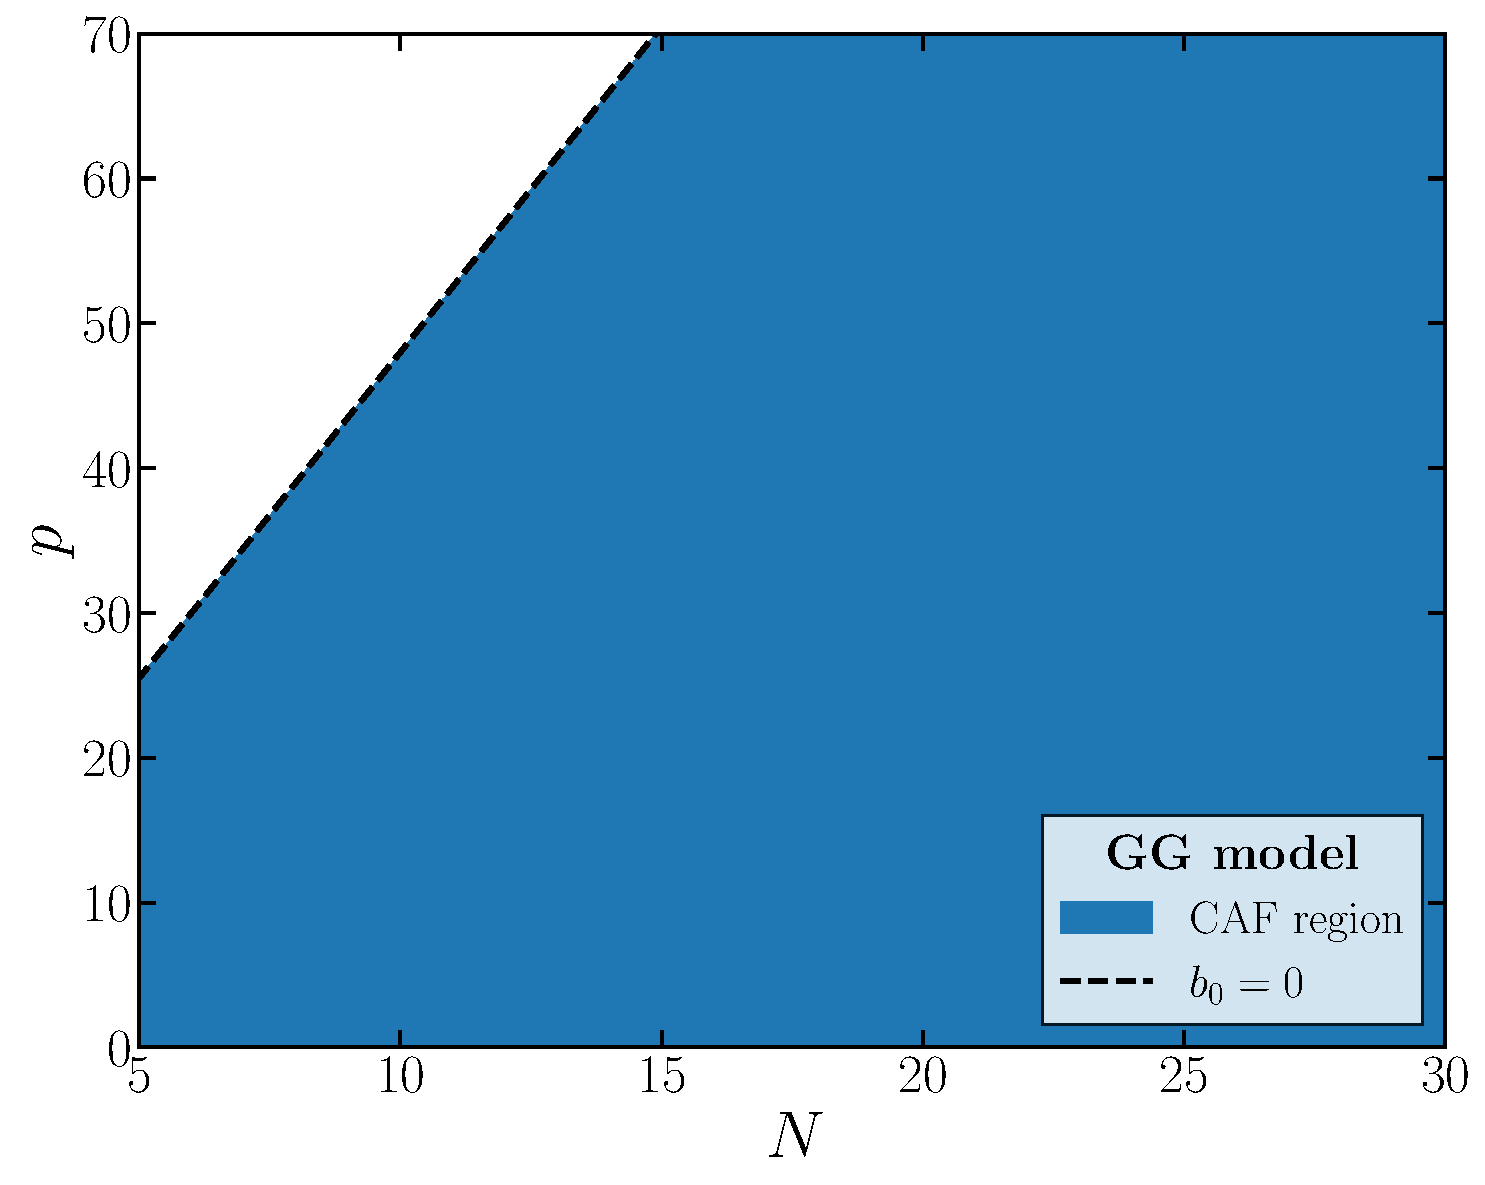
\includegraphics[width=\textwidth]{Figures/CAFGG_noscalar.pdf}
       \caption{GG model}
       \label{fig:noscalarGG}
   \end{subfigure}
   \hspace{0.1cm}
   \begin{subfigure}[b]{0.49\textwidth}
       \centering
       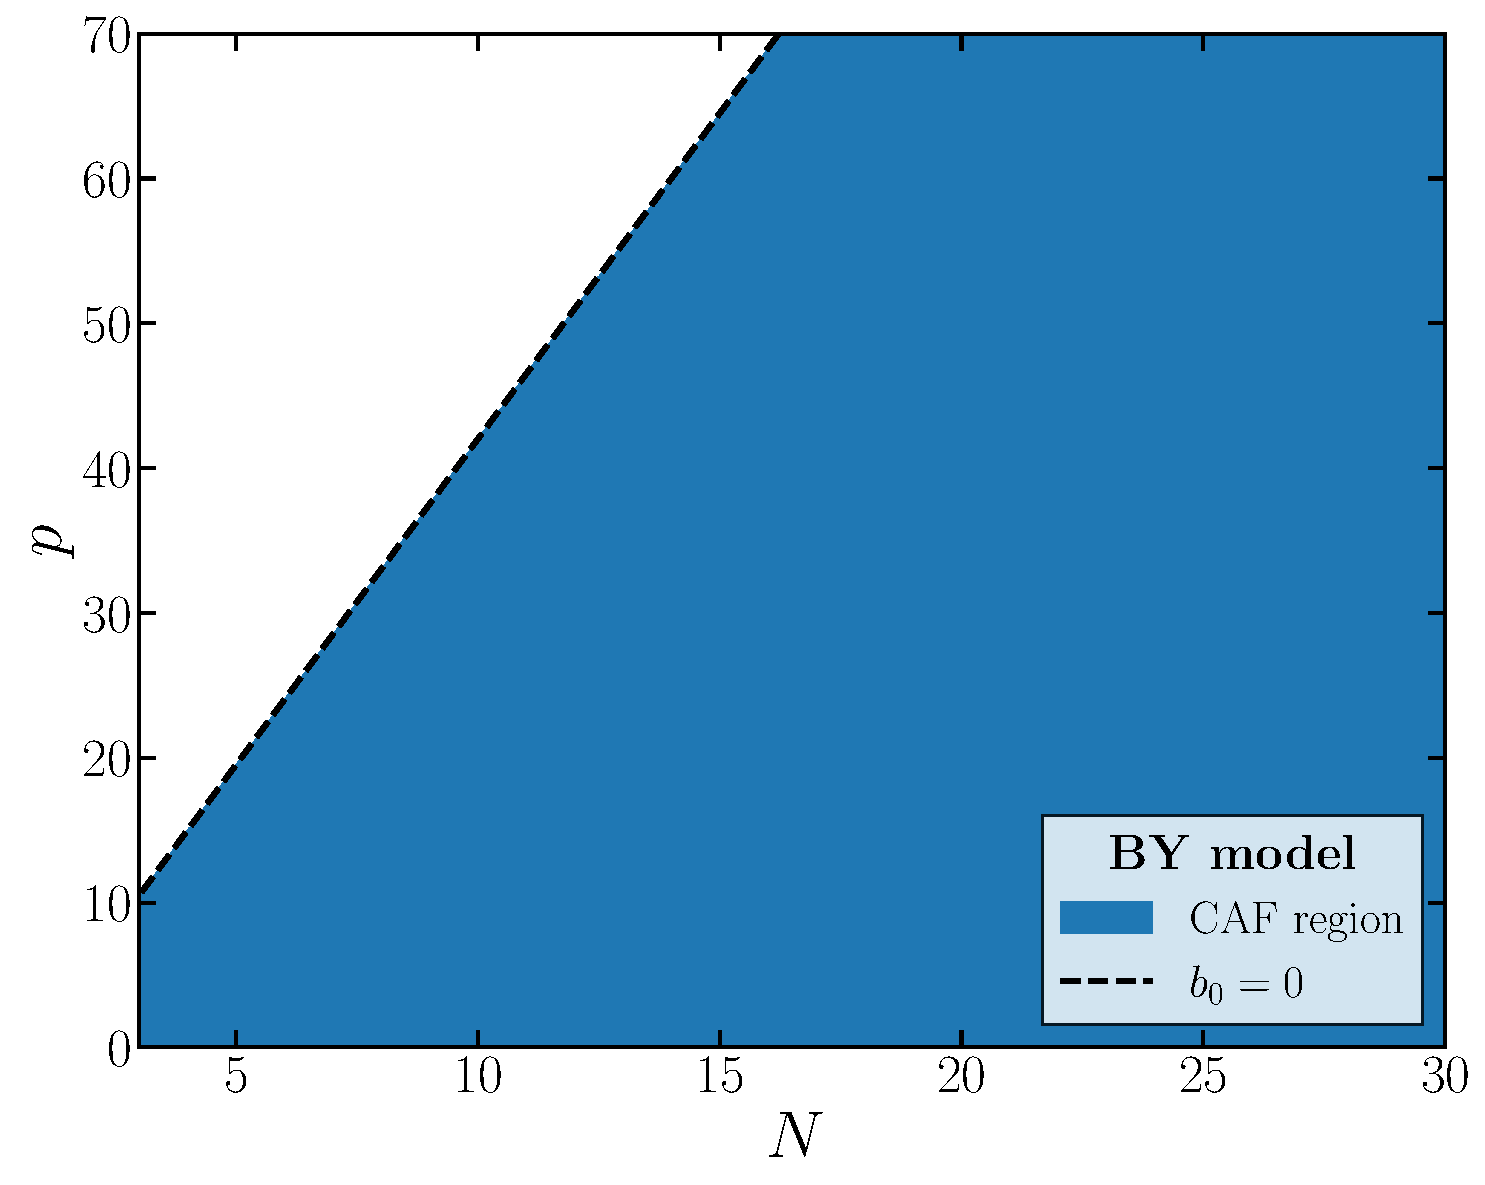
\includegraphics[width=\textwidth]{Figures/CAFBY_noscalar.pdf}
       \caption{BY model}
       \label{fig:noscalarBY}
   \end{subfigure}
   \caption{The figure illustrates the CAF region in parameter space ($N,p$) for (a) the GG model and (b) the BY model, without any scalars. The shaded blue area represents the CAF region, bounded by the dashed black line corresponding to the condition $b_0=0$. This boundary is given by the $p_{\max}$ function  Eq.~\eqref{eq:pNnoscalarGG} for the GG model and Eq.~\eqref{eq:pNnoscalarBY} for the BY model.}
   \label{fig:noscalar}
\end{figure} 
The gauge coupling thus creates an upper limit for the CAF region of the model and the GG model without scalars can therefore be CAF for all $N$, as seen in Figure~\ref{fig:noscalarGG}. 

\subsection{Scalar-Free Bars--Yankielowicz model}
We now focus on the BY model \cite{Bars:1981se}. Like the GG model, the BY model is a chiral model, the difference from the GG model is that the chiral fermion is in the two-index symmetric representation, i.e.\ $\chi_{ij}=\chi_{ji}$. This affects the anomaly coefficient of the field $A(\ytableausetup{boxsize=0.25cm}\begin{ytableau}{}&{}\end{ytableau})=(N+4)$. Effectively changing the copies of the anti-fundamental vector-like fermion to $q=N+4+p$, which ensures anomaly cancellation. This also changes the Dynkin index $T(\ytableausetup{boxsize=0.25cm}\begin{ytableau}{}&{}\end{ytableau})=\frac{N+4}{2}$, effectively changing the computation of the charges and will introduce a sign change to the $\U_1(1)$ charges, as seen in Table~\ref{tab:BY}.

Similar to the GG model, the BY model also has a lower boundary of the number of colours of the gauge group. The dimension of the two-index symmetric representation is $\frac{N(N+1)}{2}$. For $N=2$ this yields a dimension of $3$, which is the adjoint representation of the group, and thus is real \cite{Georgi:1999wka}, allowing for a Majorana mass term in the Lagrangian. For $\SU(3)$ the dimension is $6$ which is a complex representation. Resulting in a lower boundary of number of colours for the BY model: $N\ge3$. 

Thus, the Lagrangian is similar to that of the GG model and can be expressed as
\begin{align}\mathcal{L}= -\frac{1}{4} F_{\mu\nu}^a F^{a\mu\nu}+ i \bar{\chi}^{ij} \slashed{D} \chi_{ij} 
    + i \bar{\psi}^i_\alpha \slashed{D} \psi_i^\alpha 
    + i \bar{\tilde{\psi}}_i^\beta \slashed{D} \tilde{\psi}^i_\beta
    \,,
\end{align}
with similar index definitions as in Eq.~\eqref{eq:lGGnoscalar} except for the flavour index of the anti-fundamental fermion now given by $\beta=1,\dots, N+4+p$.

The gauge beta function can be found similarly to the GG model. The computation only differs in the number of anti-fundamental fermions: $N+4+p$, and the Dynkin index of the chiral fermion, yielding
\begin{align}
\sum T(R_f) &= \frac{N+2}{2} + \frac{N+4+p}{2} + \frac{p}{2} = N + 3 + p\,.
\end{align}
\begin{table}[b]
    \centering
    \renewcommand{\arraystretch}{1.5} 
    \begin{tabular}{|c|c|c|c|c|c|}
    \hline
    Fields & $\mathrm{SU}(N)$ & $\mathrm{SU}(N + 4 + p)$ & $\mathrm{SU}(p)$ & $\mathrm{U}_1(1)$ & $\mathrm{U}_2(1)$ \\
    \hline
    $\chi$ & $\ytableausetup{boxsize=0.25cm}\begin{ytableau}{}&{}\end{ytableau}$ & $1$ & $1$ & $N + 4$ & $2p$ \\

    $\tilde\psi$ & $\overline{\begin{ytableau}{}\end{ytableau}\rule{0pt}{7.5pt}}$ & $\overline{\begin{ytableau}{}\end{ytableau}\rule{0pt}{7.5pt}}$ & $1$ & $-(N + 2)$ & $-p$ \\

    $\psi$ & ${\begin{ytableau}{}\end{ytableau}}$ & $1$ & ${\begin{ytableau}{}\end{ytableau}}$ & $N +2$ & $-(N - p)$ \\
    \hline
    \end{tabular}
    \caption{Field content of the BY model. The table shows how the fields transform under the gauge and global symmetry groups, and their charges under the $\mathrm{U}_1(1)$ and $\mathrm{U}_2(1)$ symmetries.}
    \label{tab:BY} 
\end{table}
Thus, we obtain
\begin{equation}
    b_0=-\frac{2}{3}\left({9}N-6-2p\right) \,. \label{eq:betagaugeBY}
\end{equation}
This is similar the $b_0$ coefficient of the GG model in Eq.~\eqref{eq:betagauge}, up to the sign of the second term. Therefore the CAF region for the BY model is similar to that of the GG model. The conditions on the gauge beta function creates a comparable upper boundary which is given by
\begin{equation}
    p_{\text{max}}(N)=\frac{9N-6}{2} \,.\label{eq:pNnoscalarBY}
\end{equation} 
Thus, a CAF region exist for any N, as can be seen in Figure~\ref{fig:noscalarBY}.

Having now seen the two considered chiral models: the GG and the BY, it is time to introduce scalars into the mix. 

\section{Adding a Single Anti-Fundamental Scalar} \label{sec:fundscalar}
We first extend the GG and BY models with one scalar field in the anti-fundamental representation. Thus, we introduce the scalar field $\phi$ to theory, which changes our Lagrangian. We will denote the chiral fermionic field as $\Lambda_{ij}$, referring either to $\Psi_{ij}$ for the case of the antisymmetric two-index tensor of the GG model or $\chi_{ij}$ in the case of the two-index symmetric tensor of the BY model. 

These field will also have charges under the $U_1(1)$ and the $\U_2(1)$ groups. These can be found by ensuring that we can write a Yukawa term for the chiral fermion, given by
\begin{equation}
    \mathcal{L}_{\text{Yukawa}}= y^\beta\Lambda_{ij} \tilde\psi ^{i}_{\beta} \phi^j + \mathrm{h.c.}\,.\label{eq:YukawaL}
\end{equation}
For this term to be charge-neutral, the total charge under each gauge group must vanish. For the first charge, $Q_1$, we have:
\begin{align}
     Q_{1_\Lambda} + Q_{1_{\tilde{\psi}}} + Q_{1_\phi} &= 0  \\
     (N \mp 4) - (N \mp 2) + Q_{1_\phi} &= 0 \quad \implies \quad Q_{1_\phi} = \pm 2 \,,
\end{align}
where the upper (lower) sign refers to the GG (BY) model. We will use this convention henceforth. Similarly, for the second charge, $Q_2$:
\begin{align}
     Q_{2_\Lambda} + Q_{2_{\tilde{\psi}}} + Q_{2_\phi} &= 0 \notag \\
     2p - p + Q_{2_\phi} &= 0 \quad \implies \quad Q_{2_\phi} = -p \,.
\end{align}
This charge assignment prohibits Yukawa terms mixing the vector-like fermions, since they are not invariant under $\U_1(1)$ and $\U_2(1)$. We will therefore have the Yukawa coupling written in \eqref{eq:YukawaL}.

The Lagrangian will also include self-interaction of the scalars. Ensuring renormalisability and symmetry invariance, we can write terms like
\begin{equation}
    \mathcal{L}_{\text{quartic}}\sim 
    \lambda \phi^\dagger_i \phi^i \phi^\dagger_j \phi^j + (\phi_i^\dagger (T^A)^i_{\,j}\phi^j)(\phi_k^\dagger (T^A)^k_{\,l}\phi^l)\,.\label{eq:quaritcL}
\end{equation}
However, for a scalar in the (anti-)fundamental representation, the terms are not linearly independent. This can be proved by considering that the generators $T^A$ satisfy the Fierz identity (see Appendix \ref{app:Fierz} for the derivation)
\begin{align}
    T_i ^{\,A\,j}T_k ^{\,A\,l}=\frac{1}{2}\left(\delta_i^{\,l}\delta_k^{\,j}-\frac{1}{N}\delta_i^{\,j}\delta_k^{\,l}\right) \,.
\end{align}
Applying this to the second term of \eqref{eq:quaritcL} yields
\begin{align}
    \frac{1}{2} (\phi_i^\dagger \phi^j)(\phi_k^\dagger \phi^l)\left(\delta_i^{\,l}\delta_k^{\,j}-\frac{1}{N}\delta_i^{\,j}\delta_k^{\,l}\right)=\frac{1}{2}\left[\phi^{\dagger}_i \phi^j \phi^{\dagger}_j \phi^i-\frac{1}{N}\phi^{\dagger}_i \phi^i \phi^{\dagger}_k \phi^k\right]=\frac{1}{2}\left(1-\frac{1}{N}\right) (\phi^{\dagger}_i \phi^i)^2\,,
\end{align}
Thus, the two quartic terms in the Lagrangian in Eq.~\eqref{eq:quaritcL} are not linearly independent, resulting in only one quartic term. 

Having collected all the pieces we can write the full Lagrangian as
\begin{align}
    \mathcal{L}= &-\frac{1}{4} F_{\mu\nu}^a F^{a\mu\nu}+ i \bar{\Lambda}^{ij} \slashed{D} \Lambda_{ij} 
    + i \bar{\psi}^i_\alpha \slashed{D} \psi_i^\alpha 
    + i \bar{\tilde{\psi}}_i^\beta \slashed{D} \tilde{\psi}^i_\beta\\\nonumber& +(D_\mu \phi)_i^\dagger (D^\mu\phi)^i+(y^\beta\Lambda_{ij} \tilde\psi ^{i}_{\beta} \phi^j + \mathrm{h.c.})+\lambda (\phi^\dagger_i \phi^i)^2 
    \,,
\end{align}
An overview of the model and the transformation of the fields can be seen in Table~\ref{tab:fund}.
\begin{table}[ht]
    \centering
    \renewcommand{\arraystretch}{1.5} 
    \begin{tabular}{|c|c|c|c|c|c|}
    \hline
    Fields & $\mathrm{SU}(N)$ & $\mathrm{SU}(N \mp 4 + p)$ & $\mathrm{SU}(p)$ & $\mathrm{U}_1(1)$ & $\mathrm{U}_2(1)$ \\
    \hline
    $\Lambda$ & $\ytableausetup{boxsize=0.25cm, centertableaux}\begin{ytableau}{}\\{}\end{ytableau} \;\, / \;\, \begin{ytableau}{}&{}\end{ytableau}$ & 1 & 1 & $N \mp 4$ & $2p$ \\

    $\tilde\psi$ & $\overline{\begin{ytableau}{}\end{ytableau}\rule{0pt}{7.5pt}}$ & $\overline{\begin{ytableau}{}\end{ytableau}\rule{0pt}{7.5pt}}$ & 1 & $-(N \mp 2)$ & $-p$ \\

    $\psi$ & ${\begin{ytableau}{}\end{ytableau}}$ & 1 & ${\begin{ytableau}{}\end{ytableau}}$ & $N \mp 2$ & $-(N - p)$ \\
    \hline
    $\phi$ & $\overline{\begin{ytableau}{}\end{ytableau}\rule{0pt}{7.5pt}}$ & 1 & 1 & $\pm 2$ & $-p$ \\
    \hline
    \end{tabular}
    \caption{Field content of the GG (upper signs, antisymmetric $\Lambda$) and BY (lower signs, symmetric $\Lambda$) models with an anti-fundamental scalar $\phi$.  The table shows how the fields transform under the gauge and global symmetry groups, and their charges under the $\mathrm{U}_1(1)$ and $\mathrm{U}_2(1)$ symmetries. }
    \label{tab:fund} 
\end{table}

It should be noted that the Yukawa term explicitly breaks the global symmetry $\mathrm{SU}(N\mp 4+p)$. The Yukawa couplings are a vector $y^\beta$ in the flavour space and, without loss of generality, it can be rotated using a $\mathrm{SU}(N\mp4+p)$ transformation so that only its first component is non-zero.\footnote{The flavour symmetry group is therefore broken following $\mathrm{SU}(N\mp4+p) \to \mathrm{SU}(N\mp 4+p-1)$, since the rotation of the Yukawa vector to one non-zero, is the same as selecting a specific component. Thus, only the remaining perpendicular components leaves the term invariant. } Hence, physically there is a single coupling constant, which we define as $y$, which greatly simplifies the computation of the beta functions since $y_\beta y^\beta=y^2$.

We begin with the RG equation for the gauge coupling. The only change from the computation done in the previous section is the inclusion of the anti-fundamental scalar, which contributes with $T(S) = 1/2$. Using \eqref{eq:betagauge}, we obtain 
\begin{equation}
\Delta b_0^{\text{scalar}} =  \frac{2}{3} T(S) =  \frac{1}{3}\,,\label{eq:scaleff}
\end{equation}
Thus, the beta function of the gauge coupling is given by
\begin{equation}
    \beta_g=-\frac{\alpha_g^2}{3}\left(18N-4p\pm{12}-1\right)\,.\label{eq:betagwithp}
\end{equation}
 The $(-1)$ inside the bracket corresponds to the scalar contribution.

The remaining beta functions are computed using the \texttt{RGBeta} library in Mathematica \cite{Thomsen:2021ncy}. Using similar rescaled couplings as for the gauge coupling $\alpha_y=y^2/(4\pi)^2$, $\alpha_\lambda=\lambda/(4\pi)^2$, the beta functions are given by
\begin{align}
    \beta_y&= \frac{\alpha_y}{2}\left[(3 N+2\mp3)\alpha_y+6 \alpha_g\left(-3 N\pm2+\frac 5N\right) \right]\,,\label{eq:betaywithp}
   \\
   \beta_\lambda&=\alpha_\lambda\left[2(N\mp1)\alpha_y-\frac{6 \alpha_g 
   \left(N^2-1\right)}{N}+4 \alpha_\lambda (N+4)\right]\nonumber\\&\;\;\;\;\;\;-\frac{1}{2} (N+1\mp 2 )
  \alpha_y^2+\frac{3 \alpha_g^2 \left(N^3+N^2-4 N+2\right)}{4 N^2}\,. \label{eq:betalamwithp}
\end{align}
\begin{figure}[b!]
    \centering
    \begin{subfigure}[b]{0.49\textwidth}
        \centering
        
\includegraphics[width=\textwidth]{Figures/CAFGG_fund_Ng1.pdf}
        \caption{GG model} 
        \label{fig:cafgg_fund}
    \end{subfigure}
    \hspace{0.1cm}
    \begin{subfigure}[b]{0.49\textwidth}
        \centering
        
\includegraphics[width=\textwidth]{Figures/CAFBY_fund_Ng1.pdf}
        \caption{BY model} 
        \label{fig:cafby_fund}
    \end{subfigure}
    \caption{CAF regions in parameter space $(N,p)$ for (a) the GG model and (b) the BY model, with one scalar in the anti-fundamental representation. The dark blue area represents the fixed-flow CAF region, bounded above by $b_0=0$ condition (dashed black line) and for the GG model the $b_0-d_2'+\sqrt{k'}=0$ below (dotted black line). The light blue region highlights the CAF region off fixed flow bounded by the $b_0=0$ condition above and the $k=0$ (dash-dotted black line) condition below. The striped region indicates that the model exhibits CAF both on and off fixed flow.  The boundaries are given by the $p_{\max}$ and $p_{\min}$ functions  Eqs. \eqref{eq:pmaxfundoff}, \eqref{eq:pminfundoff}, and  \eqref{eq:pminfundon}.}
    \label{fig:cafby}
\end{figure}
The limits of the CAF regions can be found by considering the boundary of the three conditions $b_0=0$, $k=0$, and $b_0-d_2'+\sqrt{k'}=0$ (see Eq.s \eqref{eq:CAF} and \eqref{eq:CAFfixed}). In the off-fixed-flow regime, the two former conditions give us 
\begin{align}
    p_{\text{max}}(N)&=\frac{18N\pm12-1}{4}\label{eq:pmaxfundoff}\,,\\
   p_{\text{min}}^\text{off}(N) &= -\frac{1}{4}  \pm 3  + \frac{9}{2N}  + \frac{3}{2N} \sqrt{ 3 (N+4)(N^3 + N^2 - 4N + 2) }\,.\label{eq:pminfundoff}
\end{align}
There is also an alternative branch of the $p_{\text{min}}^\text{off}(N)$ with a minus in front of the final term, which does not border the CAF region because the change results in a negative $p \,\forall\, N$. 

The boundary functions on fixed flow has the same upper boundary as in the off-fixed-flow regime (see Eq.~\eqref{eq:pmaxfundoff}). The lower boundary found from the $b_0-d_2'+\sqrt{k'}=0$ condition (see Eq. \eqref{eq:CAFfixed}) is given by
\begin{align}
    p_{\text{min}}^\text{on}(N)&= \frac{-720 + 4N(19 + 168N + 2N^2 - 9N^3)}{16N(N - 1)(N + 4)}\nonumber\\&\quad\;+\frac{ 3\sqrt{6}\sqrt{(1 - 3N)^2(N - 1)^2(N + 4)^2(N^2 + 2N - 2)}}{16N(N - 1)(N + 4)}\label{eq:pminfundon}\,,
\end{align}
where $p_{\text{min}}^\text{on}(N)$ only bounds the GG model, as can be seen from Figure~\ref{fig:cafgg_fund}.

We have now obtained the necessary beta functions and can continue the analysis of the models by performing a CAF analysis using the conditions mentioned in Eq.~\eqref{eq:CAF} and Eq.~\eqref{eq:CAFfixed}. We deploy these conditions on the beta functions Eqs. \eqref{eq:betagwithp}, \eqref{eq:betaywithp}, and \eqref{eq:betalamwithp}. It should be noted that the CAF regions found in this analysis \textit{may} correspond to fully asymptotically free theories. Whether these solutions correspond to CAF regions also depends on initial conditions of the couplings at a given RG scale (see Figure~\ref{fig:flowplottheory}). These conditions are provided in Eqs. \eqref{eq:Yukawacondoff}, \eqref{eq:ygfixed}, \eqref{eq:CAFalpha} and \eqref{eq:CAFalphafixed}, only when these are satisfied does one realise a genuine CAF regime. 

In Figure~\ref{fig:cafby}, the results of the CAF analysis are shown in the parameter space $(N,p)$. The light blue region in both figures represents the region where the coefficients of the beta functions satisfy the CAF conditions, when the Yukawa and gauge couplings are not on fixed flow. In other words, terms proportional to the Yukawa coupling have only a subleading effect in the beta function of the quartic couplings in this region.

Another feature of Figure~\ref{fig:cafby} is the dark blue region, which extends all the way up to the dashed black line. This is the region where the CAF conditions are satisfied for the Yukawa and gauge coupling on fixed flow. Thus, in this region, neither of the couplings is subleading. As mentioned in Section \ref{chap:CAF}, on fixed flow, the coefficients $d_2'$ and $d_4'$ can change sign. This is exactly what we observe in these models, effectively rendering the CAF conditions coming from the quartic coupling trivially satisfied. Thus, the fixed-flow region closely resembles that of the models without a scalar. 

To better understand these conditions and these regions, flow diagrams have been made both within and outside of each region. These can be found in Appendix \ref{app:flow}. The analysis gives the same result as the CAF analysis and clearly illustrates how the values of the couplings at the RG scale are restricted. 

\subsection{Inclusion of Chiral Families }\label{sec:fundscalarNg}
To further explore the GG  and BY models with a scalar in the fundamental representation, we now extend the analysis to include multiple chiral families. The transformation rules of the models will be similar to those before, as shown in Table~\ref{tab:fund_Ng}. The global symmetry group due to the multiplicity of anti-fundamental fermions $\mathrm{SU}(N\mp4+p)$ will change to $\mathrm{SU}(N_g(N\mp4)+p)$ ensuring anomaly cancellation (see Eq. \eqref{eq:anomSU}). Furthermore, another group, $\mathrm{SU}(N_g)$, is added, under which the chiral fermionic field transforms, effectively adding chiral families. This will also change the terms involving the (anti-)symmetric two-index fermionic field in the Lagrangian, by introducing a new flavour index $\gamma=1,\dots,N_g$, where $N_g$ is the number of chiral families. Putting this together, we find the following Lagrangian
\begin{align}
    \mathcal{L}&=  -\frac{1}{4} F_{\mu\nu}^a F^{a\mu\nu}+ i \bar \Lambda^{ij\gamma}\slashed{D}\Lambda_{ij\gamma}
    + i \bar{\psi}^i_\alpha \slashed{D} \psi_i^\alpha 
    + i \bar{\tilde{\psi}}_i^\beta \slashed{D} \tilde{\psi}^i_\beta +(D_\mu \phi)_i^\dagger (D^\mu\phi)^i\nonumber\\&\,\quad+(y^{\beta\gamma}\Lambda_{ij\gamma} \tilde\psi ^{i}_{\beta} \phi^j + \mathrm{h.c.})+\lambda (\phi^\dagger_i \phi^i)^2 
    \,,
\end{align}
where the Yukawa coupling is a $N_g\times (N_g(N\mp4)+p)$ matrix in flavour space.

We begin by considering the gauge beta function, which is given by
\begin{equation}
    \beta_g=-\frac{22N-1\pm 12 N_g-4N_gN -4p}{3}\alpha_g^2\,,
\end{equation}
where the beta function now depends on the number of chiral families $N_g$, together with $p$ and $N$. Hence, we can derive an upper limit on $p$ as a function of $N$ and $N_g$, namely
\begin{equation} \label{eq:pmaxfundNg}
    p_{\max} (N,N_g) = \frac{22N-1\pm12N_g-4N_g N}{4}\,.
\end{equation}
When $p_{\max} < 0$, no CAF region can exist as the gauge coupling is not asymptotically free, giving an upper bound on the number of chiral generations
\begin{equation}
    N_{g} \leq \frac{22N-1}{4(N\mp 3)}\,. 
\end{equation}
\begin{table}[ht]
    \centering
    \renewcommand{\arraystretch}{1.5} 
    \begin{tabular}{|c|c|c|c|c|c|c|}
    \hline
    Fields & $\mathrm{SU}(N)$ & $\mathrm{SU}(N_g(N \mp 4) + p)$ & $\mathrm{SU}(p)$ & $\mathrm{SU}(N_g)$ & $\mathrm{U}_1(1)$ & $\mathrm{U}_2(1)$ \\
    \hline
    $\Lambda$ & $\ytableausetup{boxsize=0.25cm, centertableaux}\begin{ytableau}{}\\{}\end{ytableau} \;\, / \;\, \begin{ytableau}{}&{}\end{ytableau}$ & $1$ & $1$ &$\overline{\begin{ytableau}{}\end{ytableau}\rule{0pt}{7.5pt}}$ & $N \mp 4$ & $2p$ \\

    $\tilde\psi$ & $\overline{\begin{ytableau}{}\end{ytableau}\rule{0pt}{7.5pt}}$ & $\overline{\begin{ytableau}{}\end{ytableau}\rule{0pt}{7.5pt}}$ & 1&1 & $-(N \mp 2)$ & $-p$ \\

    $\psi$ & ${\begin{ytableau}{}\end{ytableau}}$ & 1 & ${\begin{ytableau}{}\end{ytableau}}$ & 1&$N \mp 2$ & $-(NN_g - p)$ \\
    \hline
    $\phi$ & $\overline{\begin{ytableau}{}\end{ytableau}\rule{0pt}{7.5pt}}$ & 1 & 1 &1& $\pm 2$ & $-p$ \\
    \hline
    \end{tabular}
    \caption{Field content of the GG (upper signs, antisymmetric $\Lambda$) and BY (lower signs, symmetric $\Lambda$) models with $N_g$ chiral families and one anti-fundamental scalar $\phi$.  The table shows how the fields transform under the gauge and global symmetry groups, and their charges under the $\mathrm{U}_1(1)$ and $\mathrm{U}_2(1)$ symmetries. }
    \label{tab:fund_Ng} 
\end{table}
\begin{equation}
    \beta_{y}={\alpha_y}
    \left(3\alpha_g\left(\frac{5}{N}\pm2-3N\right)
    +\alpha_y\left(\mp N_g+N_gN+\frac{2\mp1+N}{2}\right)\right)\,,
\end{equation} 
where $N_g$ comes from the trace over Yukawa couplings in the beta function.\footnote{The trace factor is $N_g$ since $N_g \le N_gN\mp N_g4+p$ for all relevant  $N$ and $p$. } Using the same assumptions, the beta function of the quartic coupling is given by
\begin{align}
    \beta_{\lambda}=&\alpha_\lambda\left[2N_g(N\mp1)\alpha_y+\left(\frac{6}{N}-6N\right)\alpha_g+4 \alpha_\lambda (N+4)\right]-\frac{N_g}{2} (N+1\mp2)
  \alpha_y^2\nonumber\\&\,+\frac{3 \alpha_g^2 \left(N^3+N^2-4 N+2\right)}{4 N^2}\,.
\end{align}
These beta functions now include a dependency on the number of chiral families, effectively changing the CAF regions from the case of one chiral family in Section \ref{sec:fundscalar}.

We can again describe the boundaries of the CAF regions using maximal and minimum $p$ functions. The $p_{\max}$ function is given by the boundary of asymptotic freedom of the gauge coupling (see Eq.~\eqref{eq:pmaxfundNg}). For off-fixed-flow regimes the minimum is found from the $k=0$ condition (Eq. \eqref{eq:CAF}), which yields
\begin{align}
    p_{\min}^\text{off}(N,N_g)&= -\frac{1}{4} + N + \frac{3\left(3 + \sqrt{3}\sqrt{8 - 14N + 5N^3 + N^4}\right)}{2N} \pm 3N_g - N N_g\,.\label{eq:pminfundNg}
\end{align}
In the case of fixed flow we have the same $p_{\max}(N,N_g)$ function, i.e.\ Eq.~\eqref{eq:pmaxfundNg}, however the lower boundary differs between the two models. The BY models CAF regions extend all the way down to $p=0$. However, for the GG model the lower boundary from the condition $b_0-d_2'+\sqrt{k'}=0$ is found to be
\begin{align}
    p_{\min}^\text{on}(N,N_g)& = \frac{1}{16} \left( 68 + \frac{180}{N} - 20N + 48N_g - 16NN_g + \frac{3\sqrt{6}\sqrt{\frac{-2 + N(2+N)}{N_g}}(1 + N + 2(-1+N)N_g)}{N} \right)\label{eq:pminfundNgon}
\end{align}
The CAF region is demonstrated for both models in Figures  \ref{fig:CAFGGNG9} and \ref{fig:CAFNG9} in the $(N,p)$ parameter space.

\begin{figure}[t!]
    \centering
    % --- Top Row ---
    \begin{subfigure}[b]{0.49\textwidth}
        \centering
        \includegraphics[width=\textwidth]{Figures/CAFGG_NG1.pdf}
        \caption{$N_g=1$} 
        \label{fig:gg_ng1}
    \end{subfigure}%
    \hspace{0.1cm}
    \begin{subfigure}[b]{0.49\textwidth}
        \centering
        \includegraphics[width=\textwidth]{Figures/CAFGG_NG3.pdf}
        \caption{$N_g=3$}
        \label{fig:gg_ng3}
    \end{subfigure}
    
    \vspace{0.5cm} 
    % --- Bottom Row ---
    \begin{subfigure}[b]{0.49\textwidth}
        \centering
        \includegraphics[width=\textwidth]{Figures/CAFGG_NG6.pdf}
        \caption{$N_g=5$} 
        \label{fig:gg_ng6}
    \end{subfigure}%
    \hspace{0.1cm}
    \begin{subfigure}[b]{0.49\textwidth}
        \centering
        \includegraphics[width=\textwidth]{Figures/CAFGG_NG9.pdf}
        \caption{$N_g=6$}
        \label{fig:gg_ng9}
    \end{subfigure}
    
    \caption{CAF regions in the ($N$, $p$) parameter space for the GG model with $N_g \in \{1, 3, 5, 6\}$ with one anti-fundamental scalar. The dark blue area indicates the region of CAF on the fixed flow, which is bounded above by the $b_0=0$ condition (dashed black line) and below by the $b_0-c_1>0$ condition (dotted black line). The light blue area highlights the region of CAF off the fixed flow, bounded strictly between $b_0=0$ (above) and $k=0$ (dash-dotted black line, below) where the striped region indicates both cases exhibit CAF. The theoretical boundary curves correspond to the $p_{\max}$ and $p_{\min}$ functions detailed in Eqs. \eqref{eq:pmaxfundNg}, \eqref{eq:pminfundNg}, and \eqref{eq:pminfundNgon}.}
\label{fig:CAFGGNG9}
\end{figure}

\begin{figure}[t!]
    \centering
    % --- Top Row ---
    \begin{subfigure}[b]{0.49\textwidth}
        \centering
        \includegraphics[width=\textwidth]{Figures/CAFplotBY_NG1.pdf}
        \caption{$N_g=1$} 
        \label{fig:by_ng1}
    \end{subfigure}% <-- Keep this % sign!
    \hspace{0.1cm}
    \begin{subfigure}[b]{0.49\textwidth}
        \centering
        \includegraphics[width=\textwidth]{Figures/CAFplotBY_NG2.pdf}
        \caption{$N_g=2$} 
        \label{fig:by_ng2}
    \end{subfigure}
    
    \vspace{0.5cm} 
    
    % --- Bottom Row ---
    \begin{subfigure}[b]{0.49\textwidth}
        \centering
        \includegraphics[width=\textwidth]{Figures/CAFplotBY_NG3.pdf}
        \caption{$N_g=3$} 
        \label{fig:by_ng3}
    \end{subfigure}% <-- Keep this % sign!
    \hspace{0.1cm}
    \begin{subfigure}[b]{0.49\textwidth}
        \centering
        \includegraphics[width=\textwidth]{Figures/CAFplotBY_NG4.pdf}
        \caption{$N_g=4$} 
        \label{fig:by_ng4}
    \end{subfigure}
    
    \caption{CAF regions in the ($N$, $p$) parameter space for the BY model for $N_g \in \{1, 2, 3, 4\}$ with one anti-fundamental scalar. The dark blue area indicates the region of CAF on the fixed flow, which is bounded above by the $b_0=0$ condition (dashed black line). The light blue area highlights the region of CAF off the fixed flow, bounded strictly between $b_0=0$ (above) and $k=0$ (dash-dotted black line, below) where the striped region indicates both cases exhibit CAF. The theoretical boundary curves correspond to the $p_{\max}$ and $p_{\min}$ functions detailed in Eqs. \eqref{eq:pmaxfundNg} and \eqref{eq:pminfundNg}}
    \label{fig:CAFNG9}
\end{figure}

As visualised in Figure~\ref{fig:CAFGGNG9} the CAF region becomes smaller as $N_g$ becomes larger, due to the positive contribution of the fermions to the $b_0$ coefficient. While the GG model is explicitly shown for $N_g=(1,3,5,6)$ it can accommodate CAF regimes with integer solutions up to $N_g={13}$. 

It is of interest to consider the case of $\mathrm{SU}(5)$ with three chiral families, which corresponds to a GUT with the Higgs multiplet scalar \cite{Georgi:1974yf} (see Section \ref{sec:SU5}). In this setup the fundamental scalar $\phi$ can break the electroweak symmetry. Our analysis shows that the GG model possesses CAF regions both on and off fixed flow. Specifically, when the Yukawa coupling is on fixed flow the smallest amount of vector-like fermions needed to realise CAF is $p=4$. However, when the Yukawa coupling is off fixed flow the requirement increases to $p=18$. This highlights the viability of the $\mathrm{SU}(5)$ GUT when supplied with a sufficient vector-like sector. 

The BY model is shown in Figure~\ref{fig:CAFNG9}. The figure displays four values of $N_g=(1,2,3,4), $ where for $N_g\ge 5$ the CAF region vanishes contrary to the GG model. In all the cases the theory exhibits CAF both on and off fixed flow. 












\section{Adding a Single Adjoint scalar} \label{sec:adj}
Consider now the case of the scalar in the adjoint representation of $\mathrm{SU}(N)$. These scalars will be $N\times N$ matrices and can be written as $\Phi=\phi^bT^b$ where the scalar field transforms as $\Phi(x)\to U(x)\Phi(x)U^\dagger(x)$ with $U(x)=e^{\alpha^a(x)T^a}\in \mathrm{SU}(N)$. The adjoint representation is a real representation, consequently rendering it neutral under Abelian groups. It has $N^2-1$ degrees of freedom. 

Including an adjoint scalar when extending the SM is particularly useful for implementing spontaneous symmetry breaking. That is, if the scalar field acquires a VEV, it can lead to spontaneous symmetry breaking, e.g.\ $\mathrm{SU}(N)\to \mathrm{SU}(N-M)\times \mathrm{SU}(M)\times \mathrm{U}(1)$ \cite{Georgi:1974yf, Li:1973mq}. 


The new representation of the scalar changes the Lagrangian to
\begin{align}
    \mathcal{L}= &-\frac{1}{4} F_{\mu\nu}^a F^{a\mu\nu}+ i \bar{\Lambda}^{ij} \slashed{D} \Lambda_{ij} 
    + i \bar{\psi}^i_\alpha \slashed{D} \psi_i^\alpha 
    + i \bar{\tilde{\psi}}_i^\beta \slashed{D} \tilde{\psi}^i_\beta\nonumber\\&+\tr((D^\mu\Phi)(D_\mu\Phi))+ (y^\beta_\alpha \tilde\psi_\beta \Phi\psi^{\alpha}+h.c.)+\lambda_1\tr(\Phi^2)^2+\lambda_2\tr(\Phi^4)
    \;.\label{eq:Ladj}
\end{align}
In comparison to the previous model in Section \ref{sec:fundscalar}, an additional quartic term can be written\footnote{For $N\in\{2,3\}$ there are completeness identities which contract the indices and make the two quartic terms proportional. This is because the determinant goes as $(\Phi^2)^N$. The result of the BY model for $N=3$ can be seen in Appendix \ref{app:BYN3}, where it is shown that the change to the Lagrangian does not effect the final conclusion, the for $N=3$ the BY model is never CAF independently of the number of chiral generations. }. The transformation rules of the model can be seen in Table \ref{tab:adj}. Note that the $\mathrm{U}_2(1)$ symmetry (depending on $p$) is explicitly broken by the Yukawa term in the Lagrangian, since the adjoint scalar is neutral under Abelian groups and thus cannot render the term invariant under $\mathrm{U}_2(1)$.  

From Eq.\ \eqref{eq:Ladj} we see that the structure of the Yukawa term is changed, compared to the previous model. It no longer includes the chiral fermionic sector, but instead couples the vector-like fermions. Similar to the model in Section \ref{sec:fundscalarNg}, the Yukawa coupling is a matrix since $\tilde\psi$ and $\psi$ transform under two different groups. The dimensions of the Yukawa matrix is $p\times (N\mp 4+p)$, assuming universality as done in Section \ref{sec:fundscalarNg}, the trace factor is given by $\min(p,(N\mp 4+p))=p$ for all relevant $N$ of the two models. With this, we find the beta functions of the model to be 
\begin{align}
    \beta_g&=-\frac{1}{3}\,\alpha_g^2\left(17N \pm 12 -4p\right)\;,\\
    \beta_{y}&=\alpha_y\left[\left(\frac 6N-6N\right) \alpha_g+ 2p \alpha_{y}+ \left(N-\frac 3N\right )\alpha_y\right]\;,\\
    \beta_{\lambda_1} &=4\frac{N^2-9}{N}\alpha_{\lambda_1}^2+12\alpha_{\lambda_1}\alpha_{\lambda_2}+4(p\alpha_{y}-3\alpha_{g})\alpha_{\lambda_1}+3N\alpha_g^2-2p\alpha_{y}^2\;,
    \\
    \beta_{{\lambda_2}}&=(7+N^2)\alpha_{\lambda_2}^2+\frac{12(3+N^2)}{N^2}\alpha_{\lambda_1}^2+\frac{4(2N^2-3)}{N}\alpha_{\lambda_1}\alpha_{\lambda_2}+4(p\alpha_{y}-3N\alpha_{g})\alpha_{\lambda_2}+18\alpha_{g}^2\;.
\end{align}
 \begin{table}[ht]
    \centering
    \renewcommand{\arraystretch}{1.5} 
    \begin{tabular}{|c|c|c|c|c|}
    \hline
    Fields & $\mathrm{SU}(N)$ & $\mathrm{SU}(N \mp 4 + p)$ & $\mathrm{SU}(p)$ & $\mathrm{U}_1(1)$  \\
    \hline
    $\Lambda$ & $\ytableausetup{boxsize=0.25cm, centertableaux}\begin{ytableau}{}\\{}\end{ytableau} \;\, / \;\, \begin{ytableau}{}&{}\end{ytableau}$ & 1 & 1 & $N \mp 4$  \\

    $\tilde\psi$ & $\overline{\begin{ytableau}{}\end{ytableau}\rule{0pt}{7.5pt}}$ & $\overline{\begin{ytableau}{}\end{ytableau}\rule{0pt}{7.5pt}}$ & 1 & $-(N \mp 2)$ \\

    $\psi$ & ${\begin{ytableau}{}\end{ytableau}}$ & 1 & ${\begin{ytableau}{}\end{ytableau}}$ & $N \mp 2$  \\
    \hline
     $\phi$ & \textbf{adj} & $1$ & $1$ & $0$  \\
    \hline
    \end{tabular}
    \caption{Field content of the GG (upper signs, antisymmetric $\Lambda$) and BY (lower signs, symmetric $\Lambda$) models with an adjoint scalar $\phi$.  The table shows how the fields transform under the gauge and global symmetry groups, and their charges under the $\mathrm{U}_1(1)$ symmetry. Note that the $\mathrm{U}_2(1)$ is explicitly broken by the Yukawa term in the Lagrangian and is therefore not added to the table. }
    \label{tab:adj} 
\end{table}

In this section we will focus on the analysis for the GG model. A similar analysis applies to the BY model with results shown in Figures  \ref{fig:gg_combined_ng1} and \ref{fig:DeltaadjGG}.

Having two quartic couplings makes the CAF analysis different from the previous models and requires root analysis of fourth degree polynomials. We use the approach described in Section \ref{sec:CAF2} and Appendix \ref{sec:appCafadj}. This framework converts the task of solving coupled differential equations to an exercise of finding real positive solutions to a fourth-degree polynomial. There are three possible scenarios of real or complex roots, depending on the parameters $N$ and $p$. In Figure \ref{fig:roots_fixed}, it is evident that only complex roots are possible when the gauge coupling is asymptotically free, i.e.\ under the dashed line. In conclusion, there are no CAF solutions for the theory. 

In the regime where the Yukawa coupling vanishes faster than $1/t$, its contribution to the scalar beta functions is subleading. The UV behaviour of the theory may then be analysed by solving the gauge–scalar subsystem on fixed flow, effectively reducing the quartic beta equations to
\begin{align}
    \beta_{{\lambda_1}} &=4\frac{N^2-9}{N}\alpha_{\lambda_1}^2+12\alpha_{\lambda_1}\alpha_{\lambda_2}-12N\alpha_{g}\alpha_{\lambda_1}+3N\alpha_g^2 \;,\label{eq:beta1yoff}
    \\
    \beta_{{\lambda_2}}&=(7+N^2)\alpha_{\lambda_2}^2+\frac{12(3+N^2)}{N^2}\alpha_{\lambda_1}^2+\frac{4(2N^2-3)}{N}\alpha_{\lambda_1}\alpha_{\lambda_2}-12N\alpha_{g}\alpha_{\lambda_2}+18\alpha_{g}^2\;.\label{eq:beta12yoff}
\end{align}
This approach was explained in Section \ref{sec:CAF2}. 

\begin{figure}[ht]
    \centering
    \begin{subfigure}[b]{0.49\textwidth}
        \centering
        
\includegraphics[width=\textwidth]{Figures/CAFplotGG_1_RootsFixed_Ng1.pdf}
        \caption{All couplings on fixed flow} 
        \label{fig:roots_fixed}
    \end{subfigure}
    \hspace{0.1cm}
    \begin{subfigure}[b]{0.49\textwidth}
        \centering
        
\includegraphics[width=\textwidth]{Figures/CAFplotGG_2_RootsNoY_Ng1.pdf}
        \caption{$\alpha_y$ off fixed flow} 
        \label{fig:roots_noy}
    \end{subfigure}
    
    \caption{ Root structure of the fourth-degree polynomial for the GG model, for (a) all couplings on fixed flow and (b) the Yukawa coupling off fixed flow. The shaded regions denote four complex roots (white), and two real and two complex roots (light green). The dashed black line illustrates the $b_0=0$ condition, underneath which the gauge coupling is asymptotic free.} 
    \label{fig:Deltaadj}
\end{figure}
We can now perform a CAF analysis of these beta functions, leading to conditions for the quartic couplings and well-defined CAF regions. This can be seen in Figure \ref{fig:roots_noy}. In this case, there is a region where both the gauge coupling is asymptotically free and there are two real and two complex roots. To have a CAF region, we also require a potential bounded from below. Thus, the quartic couplings must be positive as well as real. To determine this, we can use Descartes' rule of signs. For the region shaded in Figure \ref{fig:BYposroots} there are three sign changes resulting in one positive real root, ensuring that the theory has a CAF region.

\begin{figure}[t!]
    \centering
    
\includegraphics[width=0.5\textwidth]{Figures/CAFplotGG_3_FinalCombined_Ng1.pdf}
    \caption{CAF regions for the GG model with the Yukawa coupling $\alpha_y$ off fixed flow (light blue). The dashed black line illustrates the $b_0=0$ condition (Eq.\ \eqref{eq:pmaxadj}), and the solid black line the $\Delta=0$ for $\alpha_y$ off fixed flow \eqref{eq:Delta0noY}.}
    \label{fig:BYposroots}
\end{figure}
In Figure \ref{fig:BYposroots}, the shaded region illustrates the models CAF region with the Yukawa coupling off fixed flow. A similar result can be seen for the BY model in Figure \ref{fig:gg_combined_ng1}. 

The CAF region is bounded from the top by the condition of $b_0=0$, from which we obtain the following function
\begin{align}
    p_{\max}(N)&=\frac{17N\pm12}{4}\;. \label{eq:pmaxadj}
\end{align}
The $p_{\min}$ function comes from the condition of $\Delta=0$ (see Eqs. \eqref{eq:Delta0noY} and \eqref{eq:Delta0}), where $\Delta$ is the discriminant of the fourth degree polynomial in Eq.\ \eqref{eq:fourthdegpoly}.  

As in the case of the anti-fundamental scalar, we can extend our model to include multiple chiral families. We will do this in the following section.
\subsection{Inclusion of Chiral Families}\label{sec:adjNg}
 Let us now upgrade the model with an adjoint scalar to include chiral generations. As done in Section \ref{sec:fundscalarNg}, the gauge group will depend on the number of families $\mathrm{SU}(N_g(N\mp4)+p)$. This also changes the transformation table, see Table \ref{tab:adj_Ng}. 

We obtain the Lagrangian 
\begin{align}
   \mathcal{L}= &-\frac{1}{4} F_{\mu\nu}^a F^{a\mu\nu}+ i \bar{\Lambda}^{ij\gamma} \slashed{D} \Lambda_{ij\gamma } 
    + i \bar{\psi}^i_\alpha \slashed{D} \psi_i^\alpha 
    + i \bar{\tilde{\psi}}_i^\beta \slashed{D} \tilde{\psi}^i_\beta\nonumber\\&+\tr((D^\mu\Phi)(D_\mu\Phi))+ (y^\beta_\alpha \tilde\psi_\beta \Phi\psi^{\alpha}+h.c.)+\lambda_1\tr(\Phi^2)^2+\lambda_2\tr(\Phi^4)
    \;,
\end{align}
where again the $\mathrm{U}_2(1)$ symmetry is explicitly broken.
\begin{table}[ht]
    \centering
    \renewcommand{\arraystretch}{1.5} 
    \begin{tabular}{|c|c|c|c|c|c|}
    \hline
    Fields & $\mathrm{SU}(N)$ & $\mathrm{SU}(N_g(N \mp 4) + p)$ & $\mathrm{SU}(p)$ & $\mathrm{SU}(N_g)$ & $\mathrm{U}_1(1)$  \\
    \hline
    $\Lambda$ & $\ytableausetup{boxsize=0.25cm, centertableaux}\begin{ytableau}{}\\{}\end{ytableau} \;\, / \;\, \begin{ytableau}{}&{}\end{ytableau}$ & $1$ & $1$ &$\overline{\begin{ytableau}{}\end{ytableau}\rule{0pt}{7.5pt}}$ & $N \mp 4$ \\

    $\tilde\psi$ & $\overline{\begin{ytableau}{}\end{ytableau}\rule{0pt}{7.5pt}}$ & $\overline{\begin{ytableau}{}\end{ytableau}\rule{0pt}{7.5pt}}$ & 1&1 & $-(N \mp 2)$  \\

    $\psi$ & ${\begin{ytableau}{}\end{ytableau}}$ & 1 & ${\begin{ytableau}{}\end{ytableau}}$ & 1&$N \mp 2$ \\
    \hline
    $\phi$ & \textbf{adj} & $1$ & $1$ & $1$ & $0$  \\
    \hline
    \end{tabular}
    \caption{Field content of the GG (upper signs, antisymmetric $\Lambda$) and BY (lower signs, symmetric $\Lambda$) models with $N_g$ chiral families and adjoint scalar $\phi$.  The table shows how the fields transform under the gauge and global symmetry groups, and their charges under the $\mathrm{U}_1(1)$ symmetry. Note that the $\mathrm{U}_2(1)$ is explicitly broken by the Yukawa term in the Lagrangian and is therefore not added to the table. }
    \label{tab:adj_Ng} 
\end{table}

Since, the Yukawa interaction is does not include the chiral fermions in the case of an adjoint scalar; only the gauge beta function will change
\begin{equation}
     \beta_g=-\frac{1}{3}\left(21N \pm 12 N_g-4p-4N_gN)\right)\alpha_g^2\;.\\
\end{equation} 
\begin{figure}[t!]
    \centering
    \begin{subfigure}[b]{0.49\textwidth}
        \centering
        
\includegraphics[width=\textwidth]{Figures/CAFplotGG_1_RootsFixed_Ng3.pdf}
        \caption{Real roots on fixed flow} 
        \label{fig:roots_fixed_ng2}
    \end{subfigure}
    \hspace{0.1cm}
    \begin{subfigure}[b]{0.49\textwidth}
        \centering
        
\includegraphics[width=\textwidth]{Figures/CAFplotGG_3_FinalCombined_Ng3.pdf}
        \caption{CAF region} 
        \label{fig:final_combined_ng2}
    \end{subfigure}
    
    \caption{ Properties of the GG model with $N_g=3$ chiral families. (a) Root structure of the fourth-degree polynomial with all the couplings on fixed flow. The shaded regions denote four complex roots (white) or two real and two complex roots (light green). (b) CAF regions with the Yukawa coupling $\alpha_y$ off fixed flow (light blue). The dashed black line illustrates the $b_0=0$ condition (Eq.\ \eqref{eq:pmaxadj}), and the solid black line the $\Delta=0$ for $\alpha_y$ off fixed flow \eqref{eq:Delta0noY}.} 
    \label{fig:Ng2}
\end{figure}

It is only possible to express the upper boundary in a compact analytic form, analogous to the case of a single chiral family. In this analysis, we obtain
\begin{align}
    p_{\max}(N,N_g)=\frac{21N\pm12 N_g-4NN_g}{4}\label{eq:padjscalar}
\end{align}
where the lower boundary is described by $\Delta=0$ (see Eqs. \eqref{eq:Delta0noY} and \eqref{eq:Delta0}).

Now we can perform a CAF analysis. First, consider the case of $N_g=3$. In Figure \ref{fig:Ng2}, a similar result can be seen as that for one chiral family: we need to go off fixed flow to obtain a CAF region. Figure \ref{fig:roots_fixed_ng2} illustrates that on fixed-flow, the roots will all be complex, when considering solutions below the dashed line, i.e.\ for asymptotic free gauge coupling. In Figure \ref{fig:final_combined_ng2}, the light blue region represents the CAF region for the Yukawa coupling off fixed flow. 

\begin{figure}[t!]
    \centering
    \begin{subfigure}[b]{0.49\textwidth}
        \centering
        
\includegraphics[width=\textwidth]{Figures/CAFplotGG_1_RootsFixed_Ng5.pdf}
        \caption{Real roots on fixed flow with $N_g=5$} 
        \label{fig:roots_fixed_ng3}
    \end{subfigure}
    \hspace{0.1cm}
    \begin{subfigure}[b]{0.49\textwidth}
        \centering
        
\includegraphics[width=\textwidth]{Figures/CAFplotGG_3_FinalCombined_Ng5.pdf}
        \caption{CAF region with $N_g=5$} 
        \label{fig:final_combined_ng3}
    \end{subfigure}

     \vspace{0.5cm} 
    \begin{subfigure}[b]{0.49\textwidth}
        \centering
        
\includegraphics[width=\textwidth]{Figures/CAFplotGG_3_FinalCombined_Ng6.pdf}
        \caption{CAF region with $N_g=6$} 
        \label{fig:gg_combined_ng5}
    \end{subfigure}
    \hspace{0.1cm}
    \begin{subfigure}[b]{0.49\textwidth}
        \centering
        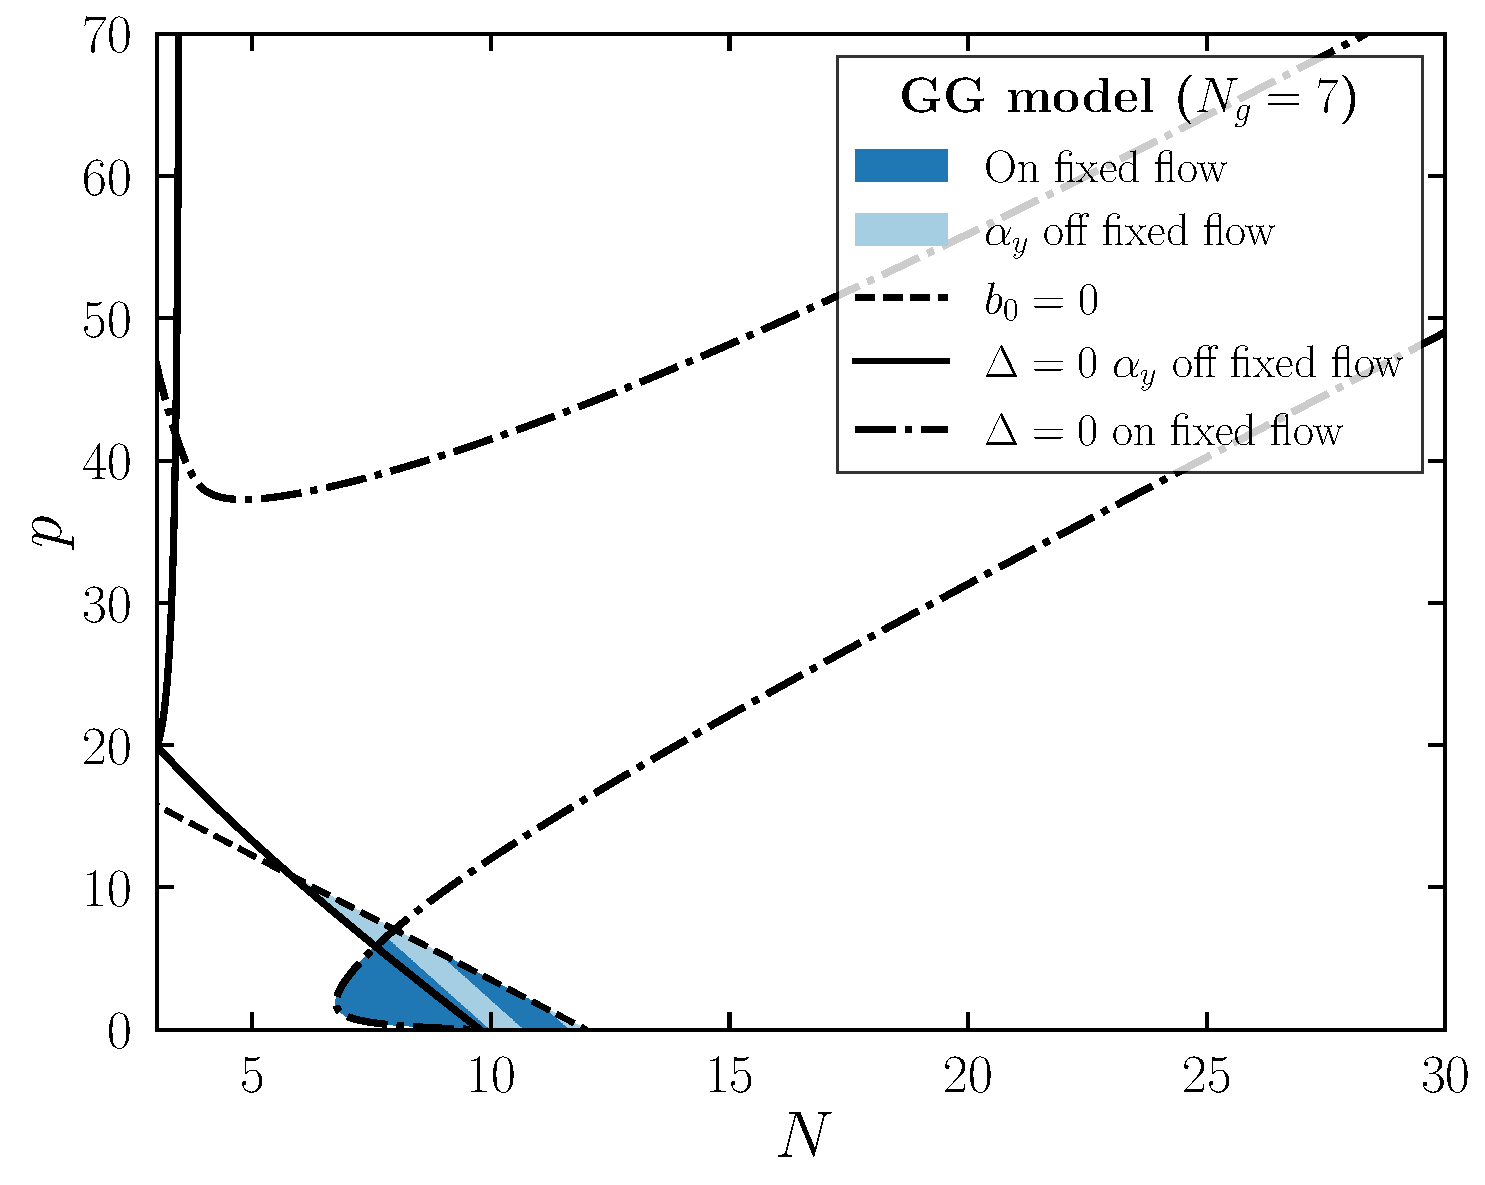
\includegraphics[width=\textwidth]{Figures/CAFplotGG_3_FinalCombined_Ng7.pdf}
        \caption{CAF region with $N_g=7$}
        \label{fig:gg_combined_ng6}
    \end{subfigure}
    
    \caption{Properties of the GG model with $N_g=5$ chiral families. (a) Root structure of the fourth-degree polynomial with all the couplings on fixed flow. The shaded regions denote four complex roots (white) or two real and two complex roots (light green). (b,c,d) CAF regions with all couplings on fixed flow (dark blue) and for the Yukawa coupling $\alpha_y$ off fixed flow (light blue). The dashed black line illustrates the $b_0=0$ condition (Eq.\ \eqref{eq:pmaxadj}), the solid black line the $\Delta=0$ for $\alpha_y$ off fixed flow \eqref{eq:Delta0noY} and the dash dotted line illustrates $\Delta=0$ on fixed flow \eqref{eq:Delta0}. } 
    \label{fig:Ng3}
\end{figure}

\begin{figure}[t!]
    \centering
    \begin{subfigure}[b]{0.49\textwidth}
        \centering
        
\includegraphics[width=\textwidth]{Figures/CAFplot_3_FinalCombined_Ng1.pdf}
        \caption{$N_g=1$} 
        \label{fig:gg_combined_ng1}
    \end{subfigure}
    \hspace{0.1cm}
    \begin{subfigure}[b]{0.49\textwidth}
        \centering
        
\includegraphics[width=\textwidth]{Figures/CAFplot_3_FinalCombined_Ng2.pdf}
        \caption{$N_g=2$} 
        \label{fig:gg_combined_ng3}
    \end{subfigure}
    
    \vspace{0.5cm} 
    \begin{subfigure}[b]{0.49\textwidth}
        \centering
        
\includegraphics[width=\textwidth]{Figures/CAFplot_3_FinalCombined_Ng3.pdf}
        \caption{$N_g=3$} 
        \label{fig:by_combined_ng5}
    \end{subfigure}
    \hspace{0.1cm}
    \begin{subfigure}[b]{0.49\textwidth}
        \centering
        
\includegraphics[width=\textwidth]{Figures/CAFplot_3_FinalCombined_Ng4.pdf}
        \caption{$N_g=4$}
        \label{fig:by_combined_ng6}
    \end{subfigure}
    
    \caption{CAF regions in the ($N$, $p$) parameter space for the BY model with $N_g \in \{1, 2, 3, 4\}$. The dark blue area indicates the region of CAF on the fixed flow, which is bounded above by the $b_0=0$ condition (dashed black line) \eqref{eq:padjscalar} and below by $\Delta=0$ (black dash dotted line) with $\alpha_y$ on fixed flow \eqref{eq:Delta0}. The light blue area highlights the region of CAF with the Yukawa coupling $\alpha_y$ off the fixed flow, bounded by the $b_0=0$ above and $\Delta=0$ below (solid black line) for $\alpha_y$ off fixed flow \eqref{eq:Delta0noY}. } 
    \label{fig:GGadjNG37}
\end{figure}
Matters change when the number of families is $N_g=5$. In Figure \ref{fig:roots_fixed_ng3}, the nature of the roots is shown, which has a region of two real and two complex roots within the region of an asymptotically free gauge coupling. Further, the polynomial has one sign change in this area, and thus has one positive real root as a consequence of Descartes' rule of signs. As seen in Figure \ref{fig:final_combined_ng3}, there is a CAF region on fixed flow.

Off fixed flow, we have a similar region to the case of $N_g=(1,2)$ and the combined CAF regions are shown in Figure \ref{fig:final_combined_ng3}, where the light blue region is the region off fixed flow and the dark blue region is on fixed flow. A similar case is that of $N_g=6,7$, which can be seen in Figure \ref{fig:gg_combined_ng5} and \ref{fig:gg_combined_ng6}. For $N_g>13$, the gauge coupling loses asymptotic freedom.

As we saw in Section \ref{sec:fundscalarNg}, the BY model exhibited CAF for $N_g<5$. The same is the case when adding an adjoint scalar. In Figure \ref{fig:GGadjNG37}, the CAF region can be seen for the case of $N_g\in\{1,2,3,4\}$.

Having examined the consequences of the Yukawa coupling off fixed flow, we now turn to a complementary scenario in the scalar sector. Specifically, we consider one quartic coupling off fixed flow and analyse whether this model exhibits CAF trajectories. Furthermore, we consider the case of both one quartic and one Yukawa coupling off fixed flow. 

% \subsection{One Quartic Scalar Coupling off Fixed Flow}
% Let us turn our focus to the scalar sector and consider one quartic coupling off fixed flow. We first take $\alpha_{\lambda_1}$ off fixed flow, effectively decoupling the quartic beta functions, we obtain
% \begin{align}
%     \beta_{{\lambda_1}} &=3N\alpha_g^2-2p\alpha_{y}^2\;,
%     \\
%     \beta_{{\lambda_2}}&=(7+N^2)\alpha_{\lambda_2}^2+4(p\alpha_{y}-3N\alpha_{g})\alpha_{\lambda_2}+18\alpha_{g}^2\;.
% \end{align}
% We can use the CAF conditions from Section \ref{sec:CAGquartic}, in Eqs. \eqref{eq:CAFfixednolam1} and \eqref{eq:CAFnotfixednolam1}. The new condition introduced in this CAF analysis for $\alpha_{\lambda_1}$ is $d_4''<0$ or $d_4<0$, depending on whether the Yukawa coupling is on or off fixed flow, respectively. In this case, $d_4=3N$, which will never be negative. Thus, a model with one adjoint scalar, which has both $\alpha_{\lambda_1}$ and $\alpha_y$ off fixed flow, cannot be CAF.
% In the case of only $\alpha_{\lambda_1}$ off fixed flow, the new condition in this model will be
% \begin{align}
%     d_4''=3N-2K\left(\frac{b_0-c_1}{c_2}\right)^2<0\;.
% \end{align}
% This condition will only be satisfied in regions where the CAF condition $k_e'<0$ holds. Thus, the theory cannot be CAF in the case of only $\alpha_{\lambda_1}$ off fixed flow. 

% In the case of $\alpha_{\lambda_2}$ off fixed flow, the condition is $e_4''<0$ and $e_4<0$. For this theory, we have the constraints
% \begin{align}
%     18&=e_4<0\;,\\
%     18&+\frac{12(3+N^2)}{N^2}\left(\frac{b_0-e_2\pm\sqrt{k_e}}{2e_1}\right)^2=e''_4<0\;.
% \end{align}
% Neither of these conditions will be satisfied for any $(N,p)$. 

% In conclusion, only with all the couplings or the Yukawa coupling $\alpha_{y}$ off fixed flow can the theory exhibit CAF. 



\chapter{Conclusion}
\label{chap:conc}
\begin{table}[ht]
\centering
\renewcommand{\arraystretch}{1.4}
\renewcommand{\tabularxcolumn}[1]{m{#1}} 

\begin{tabularx}{\textwidth}{@{}ccc >{\centering\arraybackslash}X >{\centering\arraybackslash}m{1.8cm} @{}}
\toprule
\multicolumn{1}{c}{\textbf{Model}} & \multicolumn{1}{c}{\textbf{CAF}} & \multicolumn{1}{c}{\textbf{$p(n)$}} & \multicolumn{1}{c}{\textbf{$(N,p)_{N_g}$}} & \multicolumn{1}{c}{\textbf{Figures}} \\
\midrule

\multicolumn{5}{c}{\textit{without scalars}} \\
\midrule
\rowcolor{myDarkerBlue} GG & CAF & \eqref{eq:pNnoscalarGG} & $(5,0)_1$ &--- \\

\rowcolor{myLightBlue} BY & CAF & \eqref{eq:pNnoscalarBY} & $(3,0)_1$ &--- \\


\midrule
\multicolumn{5}{c}{\textit{with one scalar in the anti-fundamental representation - all on fixed flow}} \\
\midrule
\rowcolor{myDarkerBlue} & Not CAF: $N_g > 13$ & --- & --- & --- \\
\rowcolor{myDarkerBlue} \multirow{-2}{*}{GG} & CAF: $N_g\in\{1,\dots,13\}$ &\eqref{eq:pmaxfundNg} \& \eqref{eq:pminfundNgon} & $(5,6)_1$ $(5,5)_2$ $(5,4)_3$ $(5,3)_4$ $(5,2)_5$ $(5,0)_6$ $(5,0)_7$ $(5,0)_8$ $(5,0)_9$ $(5,0)_{10}$ $(5,0)_{11}$ $(5,0)_{12}$ $(5,0)_{13}$ &\ref{fig:cafgg_fund} \& \ref{fig:CAFGGNG9}  \\

\rowcolor{myLightBlue} & Not CAF: $N_g > 4$ & --- & --- & --- \\
\rowcolor{myLightBlue} \multirow{-2}{*}{BY} & CAF: $N_g\in\{1,\dots,4\}$  & \eqref{eq:pmaxfundNg}  & $(3,0)_1$ $(3,0)_2$ $(4,0)_3$ $(9,0)_4$ &\ref{fig:cafby_fund} \& \ref{fig:CAFNG9} \\


\midrule
\multicolumn{5}{c}{\textit{with one scalar in the anti-fundamental representation - Yukawa off fixed flow}} \\
\midrule
\rowcolor{myDarkerBlue} & Not CAF: $N_g > 13$ & --- & --- & --- \\
\rowcolor{myDarkerBlue} \multirow{-2}{*}{GG} &CAF: $N_g\in\{1,\dots,13\}$  & \eqref{eq:pmaxfundNg} \& \eqref{eq:pminfundNg}& $(5,22)_1$ $(5,20)_2$ $(5,18)_3$ $(5,16)_4$ $(5,14)_5$ $(5,12)_6$ $(5,10)_7$ $(5,8)_8$ $(5,6)_9$ $(5,4)_{10}$ $(5,2)_{11}$ $(5,0)_{12}$ $(5,0)_{13}$ &\ref{fig:cafgg_fund} \& \ref{fig:CAFGGNG9} \\

\rowcolor{myLightBlue} & Not CAF: $N_g > 4$ & --- & --- & --- \\
\rowcolor{myLightBlue} \multirow{-2}{*}{BY} & CAF: $N_g\in\{1,\dots,4\}$  &\eqref{eq:pmaxfundNg} \& \eqref{eq:pminfundNg} & $(3,10)_1$ $(3,4)_2$ $(4,0)_3$ $(9,0)_4$   &\ref{fig:cafby_fund} \& \ref{fig:CAFNG9} \\

\bottomrule
\end{tabularx}
\caption{Summary of CAF possibilities for the BY and GG models for different numbers of chiral families ($N_g$). The table shows the CAF status, the boundary functions $p(N,N_g)$ for vector-like fermions, and the minimal $N$ for each $N_g$ and the required minimal $p$ displayed as as $(N,p)_{N_g}$.\label{tab:conc_part1}}
\end{table}

Chiral gauge-Yukawa theories are the cornerstone of modern particle physics, exemplified by the Standard Model (SM). Even so, the understanding of their dynamics remains out of reach in various aspects. This thesis has closed some gaps in characterising their short-distance behaviour. We  considered the generalised Georgi--Glashow (GG) and the Bars--Yankielowicz (BY) models. Their high-energy dynamics was explored with a goal of realising complete asymptotic freedom (CAF) of the couplings. To evaluate physically relevant models, we added a single scalar in either the fundamental or the adjoint representation of $\SU(N)$. Exploiting the freedom to vary these parameters, we systematically evaluated the CAF conditions of the models, distinguishing between fixed-flow and off-fixed-flow regimes. The former describes the scenario where all the couplings vanishing at the same rate as the gauge coupling in the UV, while the latter describes the case where the Yukawa coupling vanishes faster than the gauge coupling. Through this analysis we varied the multiplicity of chiral families, as well as the vector-like fermions. The additional degrees of freedom originating from this later multiplicity proved necessary to realise CAF regimes in the models. 

Through this analysis, we discovered that the possible CAF regimes can be categorised only by the relation of the Yukawa and gauge couplings, and whether they exhibit "fixed-flow" or "off-fixed-flow" behaviour. The quartic coupling cannot be off-fixed-flow alone, since this will not be physically self-consistent, due to its beta functions term proportional to $\alpha_g^2$.

The CAF analysis demonstrates that all the considered classes of models can exhibit CAF regions within specific parameter spaces defined by the number of colours, chiral families, and vector-like families. These results are summarised in Table~\ref{tab:conc_part1} for models with no scalars or one fundamental scalar and in Table~\ref{tab:conc_part2} for models with an adjoint scalar. These tables detail the model type, the flow-trajectory type, the multiplicity of chiral families, the $p$-functions describing the upper and lower bounds on the needed vector-like fermions, the minimal models (in terms of the number of colours and required vector-like families for each viable chiral family), and lastly, references to related figures. 

This classification of the chiral gauge-Yukawa models provides a framework for identifying Grand Unified Theories (GUT)s that are UV complete. A model of particular interest is the $\SU(5)$ generalised Georgi--Glashow model with three chiral families. For this model, we found that when including one fundamental scalar, CAF regimes can be achieved by adding at least 4 vector-like fermions. This ensures fixed-flow CAF-dynamics, whereas 18 vector-like fermions are required for off-fixed-flow dynamics. In contrast, no such dynamics are found when the fundamental scalar is replaced with an adjoint scalar, in this case, the minimal model with three families would be $\SU(7)$ with at least 32 vector-like fermions. Recall, that a realistic GUT must include both a Higgs like scalar (represented here by the fundamental scalar) and a scalar that breaks the gauge group down to the Standard Model gauge sector, $\SU(3)_C\times\SU(2)_L\times \U(1)_Y$. Thus, the findings of this thesis serve as a preliminary step, as a complete, realistic model would require inclusion of both scalars. Such an analysis would be complicated by the extension of the Yukawa and quartic sector.

A complete understanding of chiral gauge-Yukawa models requires an analysis of their low-energy behaviour. While the conformal window has been investigated for purely fermionic models in \cite{Appelquist:2000qg,Pica:2016krb}, further analysis is needed to understand these dynamics when scalars are introduced. 


\begin{table}[ht]
\centering
\renewcommand{\arraystretch}{1.4}
\renewcommand{\tabularxcolumn}[1]{m{#1}} 

\begin{tabularx}{\textwidth}{@{}ccc >{\centering\arraybackslash}X >{\centering\arraybackslash}m{1.8cm} @{}}
\toprule
\multicolumn{1}{c}{\textbf{Model}} & \multicolumn{1}{c}{\textbf{CAF}} & \multicolumn{1}{c}{\textbf{$p(n)$}} & \multicolumn{1}{c}{\textbf{$(N,p)_{N_g}$}} & \multicolumn{1}{c}{\textbf{Figures}} \\
\midrule
\multicolumn{5}{c}{\textit{with one scalar in the adjoint representation - all on fixed flow}} \\
\midrule
\rowcolor{myDarkerBlue} & Not CAF: $N_g \in \mathbb{N} \setminus \{5,\dots,12\}$ &--- &--- &--- \\
\rowcolor{myDarkerBlue} \multirow{-2}{*}{GG} & CAF: $N_g\in\{5,\dots,12\}$ &\eqref{eq:padjscalar} \& \eqref{eq:Delta0} & $(13,2)_5$ $(9,1)_6$ $(7,1)_7$ $(6,1)_8$ $(6,1)_9$ $(6,1)_{10}$ $(5,1)_{11}$ $(5,1)_{12}$ & \ref{fig:final_combined_ng3}, \ref{fig:gg_combined_ng5} \& \ref{fig:gg_combined_ng6}\\

\rowcolor{myLightBlue} &Not CAF: $N_g \in \mathbb{N} \setminus \{3,4\}$ &--- &--- &--- \\
\rowcolor{myLightBlue} \multirow{-2}{*}{BY} & CAF: $N_g\in\{3,4\}$ & \eqref{eq:padjscalar} \& \eqref{eq:Delta0} &$(5,1)_3$ $(10,0)_4$ &\ref{fig:by_combined_ng5} \& \ref{fig:by_combined_ng6} \\


\midrule
\multicolumn{5}{c}{\textit{with one scalar in the adjoint representation - Yukawa coupling off fixed flow}} \\
\midrule
\rowcolor{myDarkerBlue} & Not CAF: $N_g > 9$ & --- & --- & --- \\
\rowcolor{myDarkerBlue} \multirow{-2}{*}{GG} & CAF: $N_g \in \{1,\dots,9\}$ & \eqref{eq:padjscalar} \& \eqref{eq:Delta0noY} & $(7,32)_1$ $(7,28)_2$ $(7,24)_3$ $(7,20)_4$ $(7,16)_5$ $(7,12)_6$ $(7,8)_7$ $(7,4)_8$ $(7,0)_9$ & \ref{fig:BYposroots}, \ref{fig:final_combined_ng2}, \ref{fig:final_combined_ng3}, \ref{fig:gg_combined_ng5} \& \ref{fig:gg_combined_ng6}\\

\rowcolor{myLightBlue} & Not CAF: $N_g > 4$ & --- & --- & --- \\
\rowcolor{myLightBlue} \multirow{-2}{*}{BY} & CAF: $N_g \in \{1,\dots,4\}$ & \eqref{eq:padjscalar} \& \eqref{eq:Delta0noY} & $(7,26)_1$ $(7,16)_2$ $(7,6)_3$ $(10,0)_4$ &  \ref{fig:GGadjNG37} \\


% \midrule
% \multicolumn{5}{c}{\textit{with one scalar in the adjoint representation - one quartic off fixed flow}} \\
% \midrule
% \rowcolor{myDarkerBlue} GG & Not CAF: $N_g\in\mathbb{N}$ & ---&--- & ---\\ 

% \rowcolor{myLightBlue} BY & Not CAF: $N_g\in\mathbb{N}$ &--- & ---&--- \\

\bottomrule
\end{tabularx}
\caption{Summary of CAF possibilities for the BY and GG models for different numbers of chiral families ($N_g$). The table shows the CAF status, the boundary functions $p(N,N_g)$ for vector-like fermions, and the minimal $N$ for each $N_g$ and the required minimal $p$ displayed as $(N,p)_{N_g}$. \label{tab:conc_part2}}
\end{table}


\printbibliography[heading=bibintoc]
%\newpage


% --- NEW APPENDIX SEPARATOR PAGE ---
\clearpage
% Adds "Appendices" to the Table of Contents as a Chapter-level item
\addcontentsline{toc}{chapter}{Appendices} 

% Creates the physical separator page
\thispagestyle{empty} % Removes the page number from this specific page
\vspace*{\fill}
\begin{center}
    \fontsize{50}{48}\selectfont\textbf{\textcolor{chaptercolour2}{Appendices}}
\end{center}
\vspace*{\fill}
\clearpage
\clearpage
% -----------------------------------
\addtocontents{toc}{\protect\setcounter{tocdepth}{0}}
\appendix
\chapter{Group theory}
\label{app:GT}
\section{Groups}\label{app:groups}
\textit{Groups} are used as a fundamental mathematical language to describe, understand and predict symmetries and physical phenomena within physics, particularly in quantum field theory. A group $G$  is a set of elements $\{g\}$ with an operation that assigns to every pair of elements a third element within that same set. The third element must satisfy \cite{Georgi:1999wka}
\begin{enumerate}
    \item Closure: If $f,g \in G$ then $h=fg\in G$.
    \item Associativity: For all $g,\,h,\,k,\in G$, $(gh)k=g(hk)$.
    \item Identity element: There exist an element, $e\in G$ such that for all $f\in G$ we have $ef=fe=f$.
    \item Inverse element: For every $f\in G$ there exist an inverse element such that $gg^{-1}=g^{-1}g=e$.
\end{enumerate}
Groups can be interpreted more visually as a multiplication table, as seen in Table \ref{tab:Z3} (for discrete group elements), this example is for the group $\mathrm{Z}_3$.
\begin{table}[h]
    \centering
    $
    \begin{array}{c||c|c|c} % Removed the last '|' here
        \backslash & e & a & b \\
        \hline\hline
        e & e & a & b \\
        \hline
        a & a & b & e \\
        \hline
        b & b & e & a  % Removed the \hline here
    \end{array}
    $
    \caption{Multiplication table of the finite group $\mathrm{Z}_3$.}
    \label{tab:Z3}
\end{table}
A group can be both finite and infinite. $\mathrm{Z}_3$ is a \textit{finite group} because it has a finite number of group elements, whereas an \textit{infinite group} will have an infinite number of group elements. The number of elements in a finite group is called the order of the group. Thus, $\mathrm{Z}_3$ is of order $3$ \cite{Georgi:1999wka}. Groups can also be categorised by being \textit{abelian} or \textit{non-abelian}. The operation of an abelian group has an extra axiom, restricting the multiplication law
\begin{enumerate}
    \item Commutative: For all $g,h\in G$, $gh=hg$.
\end{enumerate}
From the multiplication table for $Z_3$ \ref{tab:Z3} it can be seen that the group is abelian as well. 

\section{Representation} \label{app:repersentations}
A \textit{representation} of a group $G$ is a mapping, $D$ of the elements of the group onto a set of linear operators acting on a vector space $V$. This makes the abstract group easier to realise, hence representations are matrices (for finite groups). This is useful because without this a mathematical abstract object like a group, cannot directly be understood. However, through a representation of the group, we can realise it using one of the things we understand well: matrices \cite{Georgi:1999wka}. 

The group representations are useful because they live in linear space. This also means that we can always change the representation by performing a linear transformation. The mapping $D$ need to uphold two conditions \cite{Georgi:1999wka}
\begin{itemize}
    \item The representation of the identity element $e\in G$ must yield the identity operator in the respective vector space: $D(e)=1$. 
    \item The group's multiplication law is mirrored by the multiplication of their corresponding linear operators on the vector space: $D(g_1)D(g_2)=D(g_1g_2)$.
\end{itemize}
An example of this is the 3D rotation group: $\SO(3)$. The group has a representation that consist of $3\times 3$ matrices. The dimension of a representation is defined by the dimensions of the space that it acts upon \cite{Georgi:1999wka}. In this example the dimensions is thus $3$. Each group has multiple different representations and they don't have to have the same dimensions. A representation is regular if the dimensions of the representation is the order of the group \cite{Georgi:1999wka}. 

Representations can also be described by being \textit{reducible},\textit{ completely reducible} and \textit{irreducible}. To understand these definitions, we need to first understand invariant subspaces. An invariant subspace is when all mappings $D(g)$ on any vector $w$ in the subspace $W\subset V $ maps the vector back into the subspace $W$ \cite{Georgi:1999wka}
\begin{equation}
    D(g)w\in W\quad \forall\; g\in G, w\in W\;.
\end{equation}
A representation is reducible if it has a non-trivial invariant subspace. Non-trivial meaning that it has to be an invariant subspace which is not just $\{0\}$ or the entire set of $V$. An irreducible representation (irrep) is when the representation has no non-trivial invariant subspaces. Thus you cannot "break" the representation further down. A completely reducible representation is on block diagonal form 
\begin{align}
    \begin{pmatrix}
        D_1(g) & 0      & \dots  \\
        0      & D_2(g) & \dots  \\
        \vdots & \vdots & \ddots
    \end{pmatrix}
\end{align}
and can thus be written as a direct sum of irreducible representations
\begin{equation}
    D_1\oplus D_2 \oplus \cdots\;.
\end{equation}
An important property of finite groups is that their representations always is completely reducible \cite{Georgi:1999wka}.

Another feature of representations is that they can be unitary. A representation is unitary if all $D(g)$'s are unitary, where unitarity means that the operator upholds $\mathrm{O}^\dagger=\mathrm{O}^{-1}$. All representations of finite groups are equivalent to unitary representations \cite{Georgi:1999wka}.

\section{Subgroups}
A \textit{subgroup} $H$ is a group with a set of elements which all is a part of a group $G$. Then $H$ will be a subgroup of $G$. There are two trivial subgroups of $G$, namely the identity and the group itself. Subgroups thus capture a smaller symmetry structure inside a larger symmetry \cite{Georgi:1999wka}.

\section{Young Tableaux} \label{app:youngtab}
To enable us to index and construct irreducible representation of a group we utilise permutations and combinatorics through Young tableaus. We will start by considering it for the symmetry group, before utilising it for $\SU(N)$ groups. 

The goal is thus to index a simple representation of the symmetry group $\mathrm{S}_n$ which describes all possible permutation of $n$ different objects. Let us consider the symmetry group $\mathrm{S}_4$. This groups permutes the four numbers $1,2,3,4$. It is a non-abelian group. To consider their representation theory, we can describe it using combinatorics. To do this we can use conjugacy classes of the symmetric group which has a one-to-one correspondence with the simple representations. So we need to be able to label the conjugated classes. The definition is that conjugate classes consists of all permutations with the same cycle type. A cycle type is the length of a permutation. So for an example
\begin{align}
    (1)(234)
    \label{eq:cycle}
\end{align}
would leave the first number unchanged. The second number would be changed to the third, the third to the fourth and the fourth to the second. So $1234$ would change to $1342$. This is a combination of a 1-cycle and a 3-cycle. The conjugacy classes can be used to find the irreducible representations of the group. This can be done using Young tableaux \cite{Georgi:1999wka}
\begin{align}
    \ytableausetup{boxsize=0.5cm}
    \begin{ytableau}
        {} & {}\\
        {}\\
        {}
    \end{ytableau}
\end{align}
This is the same cycle as Eq. \ref{eq:cycle}. Each cycle type is represented in columns. Here we have the first row of length three and the second has of length one. This tableau thus represents the conjugacy class $(2,1^2)$, where the first denotes the boxes in first row, and that the two following rows have one box in each . Each tableau represents a different conjugacy class, another example could be the identity element $(4)$
\begin{align}
    \ytableausetup{boxsize=0.5cm}
    \begin{ytableau}
        {} & {}& {}&{}
    \end{ytableau}
\end{align}
which is four 1-cycles. The constructions of these diagrams are bounded by 
\begin{align}
    \lambda_1\ge\lambda_2\ge...\ge\lambda_n, \quad \sum_{i=1}^n\lambda_i=n\;,
\end{align}
for $\mathrm{S}_n$ where $\lambda_i$ denotes the row considered. Each tableau not only corresponds to a conjugacy class but also an irreducible representation \cite{YoungTableaux}. The dimension of the irreducible representation can be determined from the Young tableau,by dividing $n!$ with the product of the hook-lengths $h$ of all the boxes together 
\begin{align}
   f^\lambda=\frac{n!}{\prod_{(i,j)\in \lambda}h_ij} \;,
\end{align}
where the hook-length is calculated by adding $1$ (for the box it self) with all the boxes to the right and all the boxes below. So for $\mathrm{S}_4$ with $n!=4!$ the tableaus are
\begin{align}
    \ytableausetup{boxsize=0.5cm}
    &\begin{ytableau}
        {4} & {3}& {2}&{1}
    \end{ytableau}
    \quad\quad \quad
    \begin{ytableau}
        {4} & {2}&{1}\\
        {1}
    \end{ytableau}
    \quad\quad \quad\quad
    \begin{ytableau}
        {3} & {2}\\
        {2}&{1}
    \end{ytableau}
     \quad\quad \quad\quad\quad
    \begin{ytableau}
        {4} & {1}\\
        {2}\\
        {1}
    \end{ytableau}
    \quad\quad \quad\quad
    \begin{ytableau}
        {4} \\
        {3}\\
        {2}\\
        {1}
    \end{ytableau}
    \\
    &\quad\frac{4!}{4!}=1,\quad \quad\quad\frac{4!}{4\cdot 2\cdot 1\cdot 1}=3,\quad\frac{4!}{3\cdot 2\cdot 2\cdot 1}=2,\quad\frac{4!}{4\cdot 1\cdot 2\cdot 1}=3,\quad\frac{4!}{4!}=1,
\end{align}
where the numbers inside denotes the hook-length of that box \cite{westrich2011young}. 
Now if we instead of finite groups consider the continuos groups $\SU(N)$ the Young tableaux will prove to still be useful for finding the irreps of a specific group, we will come back to this after considering the basics of Lie groups. 

\section{Lie groups} \label{app:Lie}
\textit{Lie groups} serve as an important group within physics, because they describe continuous symmetries. Unlike the some of the discrete groups which we have discussed prior to this Lie groups allow for smooth and infinitesimal transformations. Considering Noether's theorem \cite{Peskin:1995ev} this continuous symmetries will result in physical conservation laws. Additionally, if the symmetries are promoted to become local gauge symmetries, they explain structure of the interactions of the theory such as the Standard Model and Grand Unified Theories \cite{Peskin:1995ev}. 
\subsection{Non-abelian group representations}
Lie groups are continuously generated groups, where "continuously" indicates that using infinitesimal elements of the group a general element can be reached. This also requires, that the group elements are arbitrarily close to the identity. An infinitesimal element can be written \cite{Georgi:1999wka}
\begin{equation}
    g(\alpha)=1+i\alpha^aT^a + \mathcal{O}^a\;,\label{eq:inftetrans}
\end{equation}
where $T^a$ is the \textit{generators} of the group and $\alpha^a$ is the infinitesimal group parameters. The generators span the space of the infinitesimal group transformations and they obey the commutation relation
\begin{equation}
    [T^a,T^b]=if^{abc}T^c\label{eq:comTa}
\end{equation}
which is a linear combination of generators. The vector space spanned by the generators, which obey commutation are called the \textit{Lie Algebra} \cite{Peskin:1995ev}. The structure constants $f^{abc}$ obey the \textit{Jacobi identity}
\begin{equation}
    f^{ade}f^{bcd}+f^{bde}f^{cad}+f^{cde}f^{abd}=0\;.\label{eq:jacobi}
\end{equation}
The commutation relations of the Lie algebra completely defines how the group element multiply close to the identity. This is the infinitesimal transformation. Thus, gauge theories, which only consider local transformations, the physics is fully determined by its algebra. However, two different Lie groups can share their Lie algebra, thus the commutation relations are shared but they have topological differences \cite{Peskin:1995ev}. When interested in gauge theories, these global difference can be ignored. 

To ensure that we have unitary representation, we consider \textit{compact} groups. This type of groups will have a finite number of generators \cite{Peskin:1995ev}.

As previously defined a group can be both non-Abelian and Abelian (see Section \ref{app:groups}). Thus if one of the generators of the group commutes with all other generators, it generates an independent continuous Abelian group \cite{Peskin:1995ev}. This type of group is called $\U(1)$ and describes phase rotations 
\begin{align}
    \psi\to e^{i\alpha}\psi\,.
\end{align}
If the algebra cannot be divided into mutually commuting subsets of generators, then the the Lie algebra is simple and belongs to a non-Abelian group. If it is possible to divide the generators in such subsets, then we have a semi-simple algebra, and can write the group structure as a product such as $\SU(4)\times\SU(2)\times\SU(2)$ \cite{Peskin:1995ev}.  

The so-called Cartan--Killing classification of simple, compact Lie algebras lead to the discovery of few possible groups which nearly all belong to the three infinite families of \textit{classical groups} \cite{Peskin:1995ev}
\begin{enumerate}
    \item \textbf{Unitary groups} $\SU(N)$ which are unitary transformations of complex $N-$dimensional vectors. It consists of $Ñ\times N$ unitary transformations with determinant one, and has $N\times N$ Hermitian matrices $t^a$ as generators. These have to satisfy $\tr t^a=0$. There are $N^2-1$ independent matrices satisfying this \cite{Peskin:1995ev}.
    \item \textbf{Orthogonal Groups} $\SO(N)$ also known as the rotation group in $N$ dimensions, this is a subgroup of unitary $N\times N$ transformations, which preserves the symmetric inner product. There are $N(N-1)/2$ generators. 
    \item \textbf{Symplectic Groups} $\mathrm{Sp}(N)$ this is a subgroup of unitary $N\times N$ transformations, which preserves the anti-symmetric inner product.  There are $N(N+1)/2$ generators. 
\end{enumerate}
Besides these there are the \textit{exceptional} Lie algebras $\mathrm{G}_2, \mathrm{F}_4, \E_6, \E_7,$ and $\E_8$. 

We will focus on the unitary groups, as these are the focus of the thesis. 

Let us consider the trace of the product of two generators
\begin{align}
    \tr T^a_R T^b_R\equiv D^{ab}\,.
\end{align}
where the subscript $R$ denotes the irrep. We choose a basis such that the $D^{ab}$ is proportional to the identity \cite{Peskin:1995ev}
\begin{equation}
    \tr{T^a_R T^b_R}=T(R)\delta^{ab}\;,\label{eq:Dynkinindex}
\end{equation}
where $T(R)$ is the Dynkin index \cite{srednicki2006qft}, and is a constant for each irrep $R$. By multiplying Eq. \eqref{eq:comTa} with another generator $T^c_R$ on the right and evaluating the trace, we obtain an expression for the structure constant, which we can write in terms of the normalisation from Eq. \eqref{eq:Dynkinindex}
\begin{equation}
    T(R)f_{abc}=-i\tr{[T^a_R ,T^b_R]T^C_R}\,,\label{eq:stuctureconstant}
\end{equation}
because of trace cyclicity
\begin{align}
    \tr{[T^a_R ,T^b_R]T^C_R}=\tr(T^a_RT^b_RT^C_R-T^b_RT^a_RT^C_R)=\tr(T^b_RT^c_RT^a_R-T^c_RT^b_RT^a_R)=\tr{[T^b_R ,T^c_R]T^a_R}\,,
\end{align}
permutations of the indices of structure constant does not change the sign. However, interchanging indices does (due to the nature of the commutator, evident from \eqref{eq:comTa}). Thus, the structure constant is completely anti-symmetric \cite{Georgi:1999wka}.

For each irrep of the group, there will be a conjugate representation. This will be noted with a bar: $\overline R$. Using the infinitesimal transformation defined in Eq. \eqref{eq:inftetrans} we can write the complex conjugate 
\begin{align}
    \psi\to(1+i\alpha^a(T^a_R))\psi\\ \psi^*\to(1+i\alpha^a(T^a_R)^*)\psi^*\,.
\end{align}
Thus we can write the conjugate representation as $T^a_{\overline R}=-(T^a_R)^T$. This ensures that combinations of a field with its complex conjugates transforms as singlet under the gauge group \cite{Peskin:1995ev}.

The unitary group has a so-called \textit{fundamental} representation. This will be the $N-$dimensional complex vector. Hence, for $N\ge2$ this irrep will be complex, there is a corresponding independent anti-fundamental representation, which will be the $\overline N-$dimensional complex vector. 

Another type of representation which is irreducible is the adjoint representation of the group. This representation is generated from the structure constants \cite{Georgi:1999wka}
\begin{align}
    (T^a_\text{adj})_{bc}=-if_{abc}\,.
\end{align}  
This can be seen from considering the condition on the generator to satisfy the Lie algebra in Eq. \eqref{eq:comTa}. For the adjoint representation, this is just a rewriting of the Jacobi identity in Eq. \eqref{eq:jacobi} \cite{Georgi:1999wka}. Thus, the Jacobi identity proves that the adjoint representation is a valid representation. Additionally, as an artefact of the structure constants being completely anti-symmetric the representation is real. The dimensions of this representation for the unitary group is $d(\text{adj})=N^2-1$ \cite{Peskin:1995ev}.

A characteristic of the representations besides the Dynkin index is the  \textit{quadratic Casimir operator} $C_2(R)$. This factor arises when considering the operator
\begin{align}
    T^2=T^a T^a\,,
\end{align}
which commute with all generators
\begin{align}
    [T^2,T^b]=0\,.
\end{align}
This means that it is an invariant of the algebra and thus a constant for each irrep. Thus, we can write the operator as 
\begin{align}
    T^a_R T^a_R=C_2(R)\mathbb{I}\,,
\end{align}
with the dimensions of the unit matrix being the dimensions of the irrep. The two constants of the irreps are related as \cite{Peskin:1995ev}
\begin{align}
    C_2(R)=\frac{d(\text{adj})}{d(R)}T(R)\,.
\end{align}
Using the convention that 
\begin{equation}
    \tr{T^a_N T^b_N}=\frac{1}{2}\delta^{ab}\;.
    \label{eq: Dynkin index fund. rep}
\end{equation}
we can write the values of these constants for $\SU(N)$. An overview can be seen in Table \ref{tab:SUN}
\begin{table}[h]
    \centering
    \renewcommand{\arraystretch}{2.2} % Prevents fractions from looking squished
    \ytableausetup{boxsize=0.25cm, centertableaux} % Set globally once to clean up the rows
    $
    \begin{array}{c||c|c|c} % Changed lc|| to c|| to remove the ghost column
        \text{Representation} & d(R) & T(R) & C_2(R) \\
        \hline\hline
        \begin{ytableau}{}\end{ytableau} \,\;/\,\; \overline{\begin{ytableau}{}\end{ytableau}\rule{0pt}{7.5pt}} & N & \dfrac{1}{2} & \dfrac{N^2 - 1}{2N} \\
        \hline
        \mathbf{adj} & N^2 - 1 & N & N \\
        \hline
        \begin{ytableau}{}&{}\end{ytableau} & \dfrac{N(N+1)}{2} & \dfrac{N+2}{2} & \dfrac{(N-1)(N+2)}{N} \\
        \hline
        \begin{ytableau}{} \\ {}\end{ytableau} & \dfrac{(N-1)N}{2} & \dfrac{N-2}{2} & \dfrac{(N-2)(N+1)}{N} % Fixed to vertical boxes for anti-symmetric
    \end{array}
    $
    \caption{Dimensions $d(R)$, Dynkin indices $T(R)$, and quadratic Casimir invariants $C_2(R)$ for the fundamental, adjoint, two-index symmetric, and two-index anti-symmetric representations.}
    \label{tab:SUN}
\end{table}

If we now consider anti-commutator relations in place of the commutator in Eq. \eqref{eq:stuctureconstant} we have another invariant symbol 
\begin{equation}
    A(R)d^{abc}\equiv \frac 12 \tr{T^a_R\{T^b_R,T^c_R\}}\;,
\end{equation}
with $A(R)$ being the anomaly coefficient \cite{srednicki2006qft} and $d^{abc}$ being a symmetric tensor. Using the cyclic property of the trace, we have
\begin{equation}
    A(R)=-A(\bar R)\;.
    \label{eq:anomaly coefficient}
\end{equation}
For real or pseudoreal representation the anomaly coefficient is thus $A(R)=0$. Thus, for chiral theories it is non-trivial for this coefficient to vanish, ensuring an anomaly free gauge sector.


\subsection{Young tableaux for SU(N)} \label{app:youngtabSUN}
As mentioned in Section \ref{app:youngtab} the Young tableau approach can be generalised to be used to find irreps of a Lie Algebra. This is done by considering the highest weight vector, $\Lambda$ \cite{Georgi:1999wka}. This weight vector is defined from the fundamental weights $\{\eta^k\}^r_{k=1}$, which is related to the root space basis vectors \footnote{The vector-space basis of the root space is written in terms of the simple roots $\{\alpha_i\}^r_{i=1}$. This root space comes from the subalgebra of a Lie algebra: The Cartan subalgebra. This vector-space basis together with the alternative basis $\{\eta^k\}^r_{k=1}$, showing that the fundamental weights are dual with the simple roots \cite{YoungTableaux}.}
\begin{align}
    \Lambda\equiv m_1\eta^1 +...+m_r\eta^r\;,
\end{align} 
where $(m_1,..,m_r)$ are the Dynkin integers. These integers is what we use to distinguish between different irreps. Each irrep will have its own distinct values of $(m_1,..,m_r)$, where the Dynkin integers must be non-negative. To understand the irreps of a certain Lie Algebra, we can now use Young tableaux, to determine the dimensions of these irreps and the decomposition of a direct product of two irreps. We can do this by considering the value of the $m_j$'s as the number of columns of length $j$. For one single box $\begin{ytableau}{} \end{ytableau}$ we will have $m_1=1$ and $m_2,...,m_r=0$. This can also be written as $(1,0,0,...,0)$. For $(0,2,0,0,...,0)$ we would have two columns of two boxes each \cite{YoungTableaux}
\begin{align}
    \ytableausetup{boxsize=0.5cm}
    \begin{ytableau}
        {} & {}\\ {}&{}
    \end{ytableau}
\end{align}
The number of rows is restricted by the group
\begin{align}
    \text{\# of boxes} =\sum^r_{j=1}j m_j\;,
\end{align}
for $SU(N)$, $r=N-1$, this means that for $SU(4)$ e.g. the maximum number of boxes will be 3 in each column for non-trivial representations. This is because a column of $n$ boxes would correspond to the determinant representation which is simply 1 \cite{YoungTableaux}. $SU(N)$ has two invariant tensors $\delta^k_l$ and $e^{abc...n}$, this is different from other Lie algebras, and therefore the Young tableaux scheme is mostly used for $SU(N)$ \cite{YoungTableaux}. The rows describe symmetric indices, and the columns describe the antisymmetric indices.   

Now to compute the dimensions of the irrep, the hook length $h_{ij}$ is used \cite{YoungTableaux}
\begin{align}
    \dim(\Lambda)=\prod_{i,j\in \Lambda}\frac{N+j-i}{h_ij}\;,
\end{align}
where $j$ denotes column and $i$ denotes row. Using this formula, we consider an example, let us focus on the Young tableau $(1,1,0,0,...,0)$
\begin{align}
    \ytableausetup{boxsize=0.5cm}
    \dim\left(\begin{ytableau}
        {} & {}\\ {}
    \end{ytableau}\right)=\begin{ytableau}
        {N} & {M}\\ {P}
    \end{ytableau}\; \text{ divided by } \;\begin{ytableau}
        {3} & {1}\\ {1}
    \end{ytableau}=\frac{1}{3}N(N^2-1)\;,
\end{align}
where $M=N+2-1=N+1$ and $P=N+1-2=N-1$. Now that we can compute the dimensions of a specific irrep from the Young tableau, the next step is to use the Young tableaux to compute direct products. Understanding how to decompose two or more representations into a direct sum of irreps, is best shown by an example. Let us consider the direct product of $(0,0,1,0,...,0)$ and $(1,1,0,0,...,0)$
\begin{align}
    \ytableausetup{boxsize=0.5cm}
    \begin{ytableau}
        {} \\ {}\\{}
    \end{ytableau}
    \otimes \begin{ytableau}
        {a} &{a}\\ {b}
    \end{ytableau}\;,
\end{align}    
the first step is to write up the two Young tableaux for the representations in the direct product. In the second Young tableau one writes a new letter in each row, so $a,b$ in the first two, in the third row $c$, and so on. For a row with multiple boxes, all boxes in the row gets the same letter. Next, the first box (the box furthest to the top and to the right) is attached to the three boxes of the first tableau, in all possible combinations \cite{YoungTableaux}
 \begin{align}
    \ytableausetup{boxsize=0.5cm}
    \begin{ytableau}
        {} \\ {}\\{}
    \end{ytableau}
    \otimes \begin{ytableau}
        {a} &{a}\\ {b}
    \end{ytableau}=\left(
        \begin{ytableau}
        {} &{a}\\ {}\\ {}
        \end{ytableau}\oplus 
        \begin{ytableau}
        {} \\ {}\\ {}\\{a}
        \end{ytableau} 
    \right)
    \otimes \begin{ytableau}
        {a}\\ {b}
    \end{ytableau}\;.
\end{align} 
After this the next box can be attached,
 \begin{align}
    \ytableausetup{boxsize=0.5cm}
    \begin{ytableau}
        {} \\ {}\\{}
    \end{ytableau}
    \otimes \begin{ytableau}
        {a} &{a}\\ {b}
    \end{ytableau}=\left(
        \begin{ytableau}
        {} &{a}&{a}\\ {}\\ {}
        \end{ytableau}\oplus
        \begin{ytableau}
        {} &{a}\\ {}\\ {}\\{a}
        \end{ytableau}\oplus  
        \begin{ytableau}
        {} &{a}\\ {}\\ {}\\{a}
        \end{ytableau}\oplus
        \begin{ytableau}
        {} \\ {}\\ {}\\{a}\\{a}
        \end{ytableau} 
    \right)
    \otimes \begin{ytableau}
        {b}
    \end{ytableau}\;.
\end{align} 
however not all of these tableaux is allowed. Having the same letter in the same column is prohibited, thus rendering the last tableau wrong \cite{YoungTableaux}. The two middle tableaux is identical \footnote{This is where the notation of $a,b$ is important. If two tableaux have the same shape, but different letters in different boxes. They would both be kept. }, and we will only keep one, thus the expression reduces to
 \begin{align}
    \ytableausetup{boxsize=0.5cm}
    \begin{ytableau}
        {} \\ {}\\{}
    \end{ytableau}
    \otimes \begin{ytableau}
        {a} &{a}\\ {b}
    \end{ytableau}=\left(
        \begin{ytableau}
        {} &{a}&{a}\\ {}\\ {}
        \end{ytableau}\oplus
        \begin{ytableau}
        {} &{a}\\ {}\\ {}\\{a}
        \end{ytableau}
    \right)
    \otimes \begin{ytableau}
        {b}
    \end{ytableau}\;.
\end{align}
Continuing, with the last box
 \begin{align}
    \ytableausetup{boxsize=0.5cm}
    \begin{ytableau}
        {} \\ {}\\{}
    \end{ytableau}
    \otimes \begin{ytableau}
        {a} &{a}\\ {b}
    \end{ytableau}=
        \begin{ytableau}
        {} &{a}&{a}&{b}\\ {}\\ {}
        \end{ytableau}\oplus
        \begin{ytableau}
        {} &{a}&{a}\\ {}&{b}\\ {}
        \end{ytableau}\oplus
        \begin{ytableau}
        {} &{a}&{a}\\ {}\\ {}\\{b}
        \end{ytableau}\oplus
        \begin{ytableau}
        {} &{a}&{b}\\ {}\\ {}\\{a}
        \end{ytableau}\oplus
        \begin{ytableau}
        {} &{a}\\ {}&{b}\\ {}\\{a}
        \end{ytableau}\oplus
        \begin{ytableau}
        {} &{a}\\ {}\\ {}\\{a}\\{b}
      \end{ytableau}\;,
\end{align}
once again not all diagrams are allowed. The additional rule is that, when adding a box, one needs to make sure that from the right, the letter from a higher row number does not precede that of a lower row number \cite{YoungTableaux}. So in this case of $a$'s and $b$'s, we need to count the number of boxes with each letter, staring from the first row at the right, moving to the left and doing the same in the following rows. If at any point in this counting, there are more $b$'s than $a$'a, the tableau should be removed. This is the same for more $c$'s than $b$'s and so on. This also means that the first and the fourth tableau should be deleted  
\begin{align}
\begin{ytableau}
        {} \\ {}\\{}
    \end{ytableau}
    \otimes \begin{ytableau}
        {a} &{a}\\ {b}
    \end{ytableau}=
    \ytableausetup{boxsize=0.5cm}
        \begin{ytableau}
        {} &{a}&{a}\\ {}&{b}\\ {}
        \end{ytableau}\oplus
        \begin{ytableau}
        {} &{a}&{a}\\ {}\\ {}\\{b}
        \end{ytableau}\oplus
        \begin{ytableau}
        {} &{a}\\ {}&{b}\\ {}\\{a}
        \end{ytableau}\oplus
        \begin{ytableau}
        {} &{a}\\ {}\\ {}\\{a}\\{b}
      \end{ytableau}\;,
\end{align}
one continues attaching the boxes of the second tableau in the direct product onto the first, until none remains. Thus, in this example we end up with four irreps, and to check that the dimensions fit, we can calculate the dimensions of the irreps. To do this, we need to assume a group, let us take $\SU(5)$. This also, changes on of the diagrams. As mentioned previously the maximum length of a column should be $N-1$. Thus, the last diagrams first column would be invariant under $\SU(5)$, and we therefore delete it 
\begin{align}
\begin{ytableau}
        {} \\ {}\\{}
    \end{ytableau}
    \otimes \begin{ytableau}
        {} &{}\\ {}
    \end{ytableau}=
    \ytableausetup{boxsize=0.5cm}
        \begin{ytableau}
        {} &{}&{}\\ {}&{}\\ {}
        \end{ytableau}\oplus
        \begin{ytableau}
        {} &{}&{}\\ {}\\ {}\\{}
        \end{ytableau}\oplus
        \begin{ytableau}
        {} &{}\\ {}&{}\\ {}\\{}
        \end{ytableau}\oplus
        \begin{ytableau}
        {} 
      \end{ytableau}\;,
\end{align}
with the dimensions
\begin{align}
    10 \times 40 = 280+70 + 45+5 \;,
\end{align} 
where on both sides the dimension is equal to $400$, thus it is consistent. Using the Dynkin integer notation the direct product can be written as
\begin{align}
    (0,0,1) \otimes (1,2) = (1,1,1)\oplus (2,0,0,1) \oplus (0,1,0,1)\oplus (1) \;.
\end{align} 
This method is useful within physics, because it is a systematic way to decompose direct products of representations. This is especially useful GUTs, where it is needed to decompose large representations into the representations of the Standard Model.


\chapter{CAF framework}
\label{app:CAF}

\section{Detailed CAF analysis}
\subsection{CAF Analysis from Solving ODE's} \label{app:caf}
This approach considers coupled ODE's governing the beta functions, which admit analytic solutions. 
\subsubsection{Yukawa Coupling}
The RG equation, which governs the Yukawa coupling, is given by
\begin{equation}
    \mu \frac{\text{d}\alpha_y}{\text{d}\mu}=\alpha_y(c_1\alpha_g+c_2\alpha_y)\;, \label{eq:betay1loopapp}
\end{equation}
where $\alpha_y=\frac{y^2}{(4\pi)^2}$, and $c_1$, $c_2$ are constants, where in general $c_1<0$ and $c_2>0$.  


\subsubsection{Quartic Scalar Coupling}
The remaining coupling can now be added to the analysis, the self-coupling
\begin{equation}
    \mu \frac{\text{d} \alpha_\lambda}{\text{d}\mu}=\alpha_\lambda\left(d_1\alpha_\lambda + d_2\alpha_g+d_3\alpha_y\right)+d_4\alpha_g^2+d_5\alpha_y^2\;.
\end{equation}
This coupling is dependent on both the other two couplings, with the coefficients $d_1,d_3,d_4\ge0$ and $d_2,d_5\le 0$.

To solve the coupled differential equations we consider the ratio $\frac{\beta_\lambda}{\beta_g}$:
\begin{equation}
    \frac{\text{d} \alpha_\lambda}{\text{d}\alpha_g}=\frac{\alpha_\lambda}{b_0\alpha_g}\left(d_1\frac{\alpha_\lambda}{\alpha_g} + d_2+d_3\frac{\alpha_y}{\alpha_g}\right)+\frac{d_4}{b_0}+\frac{d_5\alpha_y^2}{b_0\alpha_g^2}\;.\label{eq:appodelam}
\end{equation}
Recall that the Yukawa coupling can be asymptotically free in two cases: on or off fixed flow with the gauge coupling. 

\paragraph{Case 1 $k < 0$:}
We start with the general solution to the differential equation of $\alpha_\lambda(\alpha_g)$ (Equation \ref{eq:betalamfracapp}):
\begin{align}
    \alpha_{\lambda} (\alpha_{g}) = \frac{\alpha_{g}}{2\alpha_{1}}\Bigg[ b_0& - d_2 + 
    \sqrt{-k} \tan \bigg( \frac{1}{2} \bigg( \frac{\sqrt{-k} \log (\alpha_{g})}{b_0} 
    \\-&\sqrt{-k} \bigg( 2b_0 \sqrt{-k} \tan^{-1} \bigg( \frac{(b_0 - d_2) \alpha_{g} \sqrt{-k} - 2d_1 \sqrt{-k} \alpha_{\lambda_0}}{k \alpha_{g_0}} \bigg) + k \log (\alpha_{g_0}) 
    \bigg)\bigg) \frac{1}{b_0 k} \bigg) \Bigg]\;,\nonumber
\end{align}
where the definition of $k_0$ can be used to simplify the expression, we obtain:
\begin{equation}
    \boxed{\alpha_{\lambda} = \frac{\alpha_{g}}{2d_{1}} \left[ b_0 - d_2 + \sqrt{-k} \tan\left( \frac{\sqrt{-k}}{2b_0} \log\frac{\alpha_g}{\alpha_{g_0}} - \tan^{-1}\frac{k_0}{\sqrt{-k\alpha_{g_0}}} \right) \right] , \quad k<0 }
    \label{eq:appalphalamkl0}
\end{equation}
This solution only holds for \( k < 0 \), because we want a real result. For \( k > 0 \), a different approach is required. In this case the coupling will reach a Landau pole, because of the nature of the tangent function as one varies the gauge coupling. Thus, no possible CAF regions are found when $k<0$.

\paragraph{Case 2 $k > 0$:}
For $k>0$, we rewrite the square root $\sqrt{-k} = i\sqrt{k}$ which can be inserted in the solution for $k<0$
\begin{align}
    \alpha_{\lambda}(\alpha_g) = \frac{\alpha_g}{2\alpha_1} \left[ b_0 - d_2 + i\sqrt{k} \tan \left( \frac{i\sqrt{k}}{2b_0} \log \left( \frac{\alpha_g}{\alpha_{g_0}} \right) + \tan^{-1} \left( \frac{k_0}{i\sqrt{k} \alpha_{g_0}} \right) \right) \right].
\end{align}
Using the identities \(\tan(iz) = i\tanh(z)\) and \(\tan^{-1}(iz) = i\tanh^{-1}(z)\), we rewrite the argument of the tangent. Let
\begin{align}
z = \frac{\sqrt{k}}{2b_0} \log \left( \frac{\alpha_g}{\alpha_{g_0}} \right) + \tanh^{-1} \left( \frac{k_0}{\sqrt{k} \alpha_{g_0}} \right).
\end{align}
Using the identity and substituting back in, we obtain:
\begin{align}
\alpha_{\lambda}(\alpha_g) = \frac{\alpha_g}{2\alpha_1} \left[ b_0 - d_2 - \sqrt{k} \tanh(z) \right],
\end{align}
To express the hyperbolic tangent of a sum, the following relation is used
\begin{align}
\tanh(A+B) = \frac{\tanh(A) + \tanh(B)}{1 + \tanh(A)\tanh(B)}\;,
\end{align}
where
\begin{align}
A = \frac{\sqrt{k}}{2b_0} \log \left( \frac{\alpha_g}{\alpha_{g_0}} \right), \quad 
B = \tanh^{-1} \left( \frac{k_0}{\sqrt{k}\alpha_{g_0}} \right)\;.
\end{align}
Further, using the definition of $\tanh\left(x\right)=\frac{e^{2x}-1}{e^{2x}+1}$, the hyperbolic tangent of $A+B$ is thus
\begin{align}
    \tanh(A+B)=&\frac{ \frac{ \left( \frac{\alpha_g}{\alpha_{g_0}}\right)^{\frac{\sqrt{k}}{b_0}} - 1 }{ \left(\frac{\alpha_g}{\alpha_{g_0}} \right)^{\frac{\sqrt{k}}{b_0}} + 1 } + \frac{k_0}{\sqrt{k} \alpha_{g_0}} }{ 1 +\frac{ \left( \frac{\alpha_g}{\alpha_{g_0}} \right)^{\frac{\sqrt{k}}{b_0}} - 1 }{ \left(\frac{\alpha_g}{\alpha_{g_0}} \right)^{\frac{\sqrt{k}}{b_0}} + 1 }  \frac{k_0}{\sqrt{k} \, \alpha_{g_0}} }
    = \frac{
  \left( \left( \frac{\alpha_g}{\alpha_{g_0}}  \right)^{\frac{\sqrt{k}}{b_0}} - 1 \right) 
  + \frac{k_0}{\sqrt{k}\alpha_{g_0}} \left( \left( \frac{\alpha_g}{\alpha_{g_0}} \right)^{\frac{\sqrt{k}}{b_0}} + 1 \right)
}{
  \left( \left( \frac{\alpha_g}{\alpha_{g_0}}  \right)^{\frac{\sqrt{k}}{b_0}} + 1 \right) 
  + \frac{k_0}{\sqrt{k} \, \alpha_{g_0}} \left( \left( \frac{\alpha_g}{\alpha_{g_0}}  \right)^{\frac{\sqrt{k}}{b_0}} - 1 \right)
}.\nonumber
\\&=  \frac{
   (k_0+\sqrt{k}\alpha_{g_0})+(k_0- \sqrt{k}\alpha_{g_0})\left(  \frac{\alpha_g}{\alpha_{g_0}}  \right)^{-\frac{\sqrt{k}}{b_0}}
}{
  (k_0+\sqrt{k}\alpha_{g_0})-(k_0- \sqrt{k}\alpha_{g_0} )\left(  \frac{\alpha_g}{\alpha_{g_0}}  \right)^{-\frac{\sqrt{k}}{b_0}} 
}.
\end{align}
Which gives the solution for $k>0$
\begin{equation}
    \boxed{\alpha_{\lambda} = \frac{\alpha_g}{2d_1} \left( b_0 - d_2 - \sqrt{k} \, \frac{ (k_0 + \sqrt{k}\alpha_{g_0}) + (k_0 - \sqrt{k}\alpha_{g_0}) \left( \frac{\alpha_g}{\alpha_{g_0}} \right)^{\sqrt{k}/b_0} }{ (k_0 + \sqrt{k}\alpha_{g_0}) - (k_0 - \sqrt{k}\alpha_{g_0}) \left( \frac{\alpha_g}{\alpha_{g_0}} \right)^{\sqrt{k}/b_0} } \right) , \quad k>0 }
    \label{eq:appalphalamkg0}
\end{equation}



\paragraph{Case 3 $k = 0$:}
To find the solution of the last case $\lim_{k \to 0^-}(\alpha_\lambda)$ we consider the solution $k<0$ (see Eq.\ \eqref{eq:alphalamkg0}), with the approximation $\sqrt{-k} =\epsilon\ll1$. The argument of $\tan^{-1}$ is then
\begin{align}
z &= -\tan^{-1}\left( \frac{k_0}{\epsilon\alpha_{g_0}} \right) + \frac{\epsilon}{2b_0} \log\frac{\alpha_g}{\alpha_{g_0}} .
\end{align}
Using that for large $z$, $\tan^{-1}(z) = \frac{\pi}{2} - \frac{1}{z} + O(z^{-3})$, we have
\begin{align}
z = -\frac{\pi}{2} +\epsilon\left( \frac{\alpha_{g_0}}{k_0} + \frac{1}{2b_0}\log\frac{\alpha_g}{\alpha_{g_0}}\right) + O(\epsilon^3) .
\end{align}
Let us call the second term for $\epsilon A$ where $A = \frac{\alpha_{g_0}}{k_0} + \frac{1}{2b_0}\log\frac{\alpha_g}{\alpha_{g_0}}$. Then for $\epsilon$ small
\begin{align}
\tan z = \tan\left(-\frac{\pi}{2} + \epsilon A\right) = -\cot\epsilon A = -\frac{1}{\epsilon A} + O(\mu) = -\frac{1}{\epsilon A} + O(\epsilon) .
\end{align}
Using that in front of tangent, there is a factor $\sqrt {-k}=\epsilon$
\begin{align}
\epsilon \tan z = \epsilon \left( -\frac{1}{\epsilon A} + O(\epsilon) \right) = -\frac{1}{A} + O(\epsilon^2) .
\end{align}
Inserting this back in the expression for $\alpha_\lambda$, we find
\begin{align}
\alpha_{\lambda} = \frac{\alpha_g}{2d_1} \left( b_0 - d_2 - \frac{1}{A} \right) = \frac{\alpha_g}{2d_1} \left( b_0 - d_2 - \frac{1}{ \frac{\alpha_{g_0}}{k_0} + \frac{1}{2b_0}\ln\frac{\alpha_g}{\alpha_{g_0}} } \right) .
\end{align}
From this we can impose the initial condition $\alpha_{\lambda} (\alpha_{g_0}) = \alpha_{\lambda0}$ to be
\begin{align}
\alpha_{\lambda0} = \frac{\alpha_{g_0}}{2d_1} \left( b_0 - d_2 - \frac{k_0}{\alpha_{g_0}} \right) .
\end{align}
This gives us an expression for $\frac{\alpha_{g_0}}{k_0}$ which we find to be
\begin{align}
    \frac{\alpha_{g_0}}{k_0} = \frac{1}{b_0 - d_2 - \frac{2d_1\alpha_{\lambda0}}{\alpha_{g_0}}} \;.\label{eq:appk0def}
\end{align}
Inserting this back into the expression for $\alpha_\lambda$ and simplifying, we obtain
\begin{align}
    \alpha_\lambda &= \frac{\alpha_g}{2d_1} \left[ b_0 - d_2 - \frac{1}{\frac{1}{\frac{-2d_1\alpha_{\lambda_0}}{\alpha_{g_0}} + b_0 - d_2}+ \frac{1}{2b_0} \ln \frac{\alpha_q}{\alpha_{g_0}}}  \right]\;,\nonumber
    \\&=\frac{\alpha_g}{2d_1} \left[ \frac{\frac{4b_0d_1\alpha_{\lambda_0}}{\alpha_{g_0}}+\left(\frac{-2d_1\alpha_{\lambda_0}}{\alpha_{g_0}} + b_0 - d_2\right)\ln \frac{\alpha_g}{\alpha_{g_0}}(b_0-d_2)}{{2b_0} + \left(\frac{-2d_1\alpha_{\lambda_0}}{\alpha_{g_0}} + b_0 - d_2\right) \ln \frac{\alpha_g}{\alpha_{g_0}}} \right]\label{eq:appk0}
\end{align}
Using the definition of $k_0$ in Eq.\ \eqref{eq:appk0def}, Eq.\ \eqref{eq:appk0} simplifies to
\begin{equation}
    \boxed{\alpha_{\lambda} = \frac{\alpha_g}{2d_1} \frac{ 4b_0 d_1 \alpha_{\lambda0} + k_0 (b_0 - d_2) \ln\frac{\alpha_g}{\alpha_{g_0}} }{ 2b_0 \alpha_{g_0} + k_0 \ln\frac{\alpha_g}{\alpha_{g_0}} } , \quad k=0 }
    \label{eq:appalphalamkeq0}
\end{equation}
We have now obtained the last of the analytic solutions to Eq.\ \eqref{eq:betalamfracapp}, and we can move forward with the final CAF analysis. 










\subsection{CAF Analysis Using the Fixed-Flow Framework} 
To utilise the fixed-flow approach, we redefine the couplings 
\begin{equation}
    \alpha_{g_i} = \frac{\tilde \alpha_{g_i}}{t}, \quad \quad  \alpha_{y_a} = \frac{\tilde \alpha_{y_a}}
    {t}, \quad \quad \alpha_{\lambda_m} = \frac{\tilde \alpha_{\lambda_m}}{t} \;.
\end{equation}
This gives us the following equations to solve
\begin{equation}
     \boldsymbol{x}_\infty=\begin{pmatrix}
        -\beta_{{\boldsymbol{g}}}(\tilde\alpha_{g\infty})\\-\beta_{{\boldsymbol{y}}}(\tilde\alpha_{g\infty},\tilde\alpha_{y\infty})\\-\beta_{\boldsymbol{\lambda}}(\tilde\alpha_{g\infty},\tilde\alpha_{y\infty},\tilde\alpha_{\lambda\infty})
    \end{pmatrix}\label{eq:solCAF2app}\;,
\end{equation}
effectively transforming the coupled ODE's to polynomial equations. 
\subsubsection{Two Quartic Couplings}\label{sec:appCafadj}
Using Eq.\ \eqref{eq:solCAF2app} we can write the polynomial equation for the quartic scalar coupling as
\begin{equation}
    \tilde\alpha_{\lambda _{m\infty}} + d^{\lambda}_{mnp}\tilde\alpha_{\lambda _{m\infty}}\tilde\alpha_{\lambda _{p\infty}}+ \tilde\alpha_{\lambda _{m\infty}}(d^{\lambda y}_m \tilde\alpha_{y _{\infty}} +d^{\lambda_g}_m\alpha_{y _{\infty}}) + d^{y}_m\alpha_{y\infty}^2+ d^{g}_m \alpha_{g\infty}^2 = 0    \;.\label{eq:CAF2quarticapp}
\end{equation}
We consider the case of $m=1,2$ corresponding to two quartic couplings. In this case, the algebraic equation \eqref{eq:CAF2quartic} can be written as two coupled quadratic equations
\begin{equation}
    a  {x}^2 + b  {z}^2 + c  {x}{z} + d  {x} + e = 0\;,
\end{equation}
\begin{equation}
    f  {z}^2 + g  {x}^2 + h  {x}{z} + i  {z} + j = 0\;,\label{eq:CAF2poly2app}
\end{equation}
where $x=\alpha_{\lambda_{1\infty}}$ and $z=\alpha_{\lambda_{2\infty}}$. The coefficients are given by
\begin{align}
    a=d^{\lambda}_{mmm},\quad b=d^{\lambda}_{mnn},\quad c=d^{\lambda}_{mmn},\quad d=(d^{\lambda y}_m \tilde\alpha_{y _{\infty}} +d^{\lambda_g}_m\tilde\alpha_{g _{\infty}}),\quad e=d^{y}_m\alpha_{y\infty}^2+ d^{g}_m \alpha_{g\infty}^2\;,\label{eq:coef2quarticapp}
\end{align}
where $m=1$ and $n=2$. For Eq.\ \eqref{eq:CAF2poly2app}, the coefficients $f$, $g$, $h$, $i$, and $j$ are defined analogously by exchanging the indices $m\Longleftrightarrow n$ of the coefficients in Eq.\ \eqref{eq:coef2quarticapp}. 


The relevant case for our models has $b=0$
\begin{equation}
    a  {x}^2  + c  {x}{z} + d  {x} + e = 0 \;,   \label{eq:poly1}
\end{equation}
\begin{equation}
   f  {z}^2 + g  {x}^2 + h  {x}{z} + i  {z} + j = 0 \;. \label{eq:poly2}
\end{equation}
To determine whether there is any CAF region in this case, we must find the roots of the functions. This is done by inserting  ${z}$ in \ref{eq:poly1} into \ref{eq:poly2} and multiplying with $(d{x})^2$
\begin{equation}
    fT^2+gd^2 {x}^4 -hdT^2 {x}^2-idT  {x} +jd^2 {x}^2=0\;,
\end{equation}
where $T=ax^2+cx+e$. We have now obtained an uncoupled fourth-degree polynomial which we can express as
\begin{equation}
    \alpha  {x}^4  + \beta {x}^3 + \gamma  {x}^2 + \delta x+ \epsilon = 0  \;,  \label{eq:poly4th}
\end{equation}
where 
\begin{align}
&\alpha=fa^2+gd^2-had\;, \quad\beta= 2fac-hcd-iad\;, \quad\gamma=fc^2+2fae-hed-icd+jd^2\;, \\&\delta=e(2fc-id)\;, \quad\epsilon=fe^2\;.
\end{align}
By computing the sign of its determinant $\Delta$, given by \cite{Gellert1977}
\begin{align}
    \Delta = \ & 256\alpha^3 \epsilon^3 - 192\alpha^2 \beta\delta\epsilon^2 - 128\alpha^2 \gamma^2 \epsilon^2 + 144\alpha^2 \gamma\delta^2 \epsilon - 27\alpha^2 \delta^4 \\
& + 144\alpha\beta^2 \gamma\epsilon^2 - 6\alpha\beta^2 \delta^2 \epsilon - 80\alpha\beta\gamma^2 \delta\epsilon + 18\alpha\beta\gamma\delta^3 + 16\alpha\gamma^4 \epsilon \\
& - 4\alpha\gamma^3 \delta^2 - 27\beta^4 \epsilon^2 + 18\beta^3 \gamma\delta\epsilon - 4\beta^3 \delta^3 - 4\beta^2 \gamma^3 \epsilon + \beta^2 \gamma^2 \delta^2
\end{align}
one can find whether the solutions are real or complex. This depends on the following conditions \cite{Hansen:2017pwe}
\begin{itemize}
    \item For $\Delta < 0$, the polynomial will have two distinct real roots and two complex roots.
    \item For $\Delta > 0$, the polynomial has four real or complex roots.
    \begin{itemize}
        \item For $P < 0 \wedge  D < 0$: four real roots
        \item If $P > 0 \vee D > 0$: four complex roots.
    \end{itemize}
\end{itemize}
Where 
\begin{align}
    P &= 8\alpha\gamma - 3\beta^2\\
    D &= 64\alpha^3 \epsilon - 16\alpha^2 \gamma^2 + 16\alpha\beta^2 \gamma - 16\alpha^2 \beta\delta - 3\beta^4
\end{align}

Additionally, one should check whether the roots are real-positive or real-negative roots, which can be done using Descartes' rule of signs.

\paragraph{The determinant}of the quartic polynomial for the model described in sections \ref{sec:adj} and \ref{sec:adjNg} can be found using the beta functions of the theories and the definition of the coefficients of the polynomial. The boundary of the CAF region for both off and on fixed flow is found from the condition $b_0=0$ (Eqs. \eqref{eq:pmaxadj} and \eqref{eq:padjscalar}) and $\Delta=0$. The condition $\Delta=0$ with the Yukawa coupling off fixed flow is given by
\begin{align}
 \Delta=&-2176782336 N^4 P_0 - 725594112 A N^3 P_1 - 10077696 A^2 N^2 P_2 - 15116544 A^3 N P_3  \notag \\
&- 34992 A^4 P_4 - 139968 A^5 N P_5- 216 A^6 P_6 - 288 A^7 N P_7 - A^8 P_7  = 0\;,\label{eq:Delta0noY}
\end{align}
where $A = N (-21 + 4 N_g) + 4 (\mp3 N_g + p)$ and the polynomials are given by
\begin{align}
P_0 &= -217326564 - 56077596 N^2 + 23223267 N^4 - 2630538 N^6 + 166727 N^8 \notag\\&\;\;\;\;\; - 9548 N^{10} + 188 N^{12}\;, \\
P_1 &= -33434856 + 10958328 N^2 + 7518420 N^4 - 1773243 N^6 + 171254 N^8 \notag\\&\;\;\;\;\;- 9917 N^{10} + 350 N^{12}\;, \\
P_2 &= -64297800 + 83041848 N^2 + 15587964 N^4 - 10068291 N^6 \notag\\&\;\;\;\;\;+ 1385624 N^8 - 104921 N^{10} + 4472 N^{12} \;,\\
P_3 &= -571536 + 1910304 N^2 - 245412 N^4 - 262236 N^6 + 52675 N^8 - 5338 N^{10} + 247 N^{12} \\
P_4 &= -1714608 + 14362272 N^2 - 8214156 N^4 - 2139588 N^6 + 725257 N^8 \notag\\&\;\;\;\;\;- 98878 N^{10} + 4837 N^{12} \;,\\
P_5 &= 35964 - 46278 N^2 - 2949 N^4 + 3476 N^6 - 629 N^8 + 32 N^{10}\;, \\
P_6 &= 107892 - 365634 N^2 + 31473 N^4 + 27116 N^6 - 6143 N^8 + 320 N^{10}\;, \\
P_7 &= (-5 + N^2)^2 (-81 - 18 N^2 + 2 N^4)\;.
\end{align}
On fixed flow, we obtain
\begin{align} \Delta=&- B^4 D^2 N^2 (1 + N^2)^2 P_3^2 + B^2 D^3 N (7 + N^2) P_3^2 \nonumber\\ & - 64 C B^6 N^3 (1 + N^2)^3 P_3^3 + 72 C B^4 D N^2 (1 + N^2) (7 + N^2) P_3^3 + 432 C^2 B^4 N^2 (7 + N^2)^2 P_3^4 \nonumber\\& + B^2 D^3 N (1 + N^2)^2 P_4  - D^4 (7 + N^2) P_4 + 72 C B^4 D N^2 (1 + N^2)^3 P_3 P_4\nonumber \\ & - 80 C B^2 D^2 N (1 + N^2) (7 + N^2) P_3 P_4 + 96 C^2 B^4 N^2 (1 + N^2)^2 (7 + N^2) P_3^2 P_4 \label{eq:Delta0}\\ & - 576 C^2 B^2 D N (7 + N^2)^2 P_3^2 P_4 + 432 C^2 B^4 N^2 (1 + N^2)^4 P_4^2\nonumber\\& - 576 C^2 B^2 D N (1 + N^2)^2 (7 + N^2) P_4^2  + 128 C^2 D^2 (7 + N^2)^2 P_4^2  \nonumber\\&- 3072 C^3 B^2 N (1 + N^2) (7 + N^2)^2 P_3 P_4^2 - 4096 C^4 (7 + N^2)^3 P_4^3  = 0 \;,\nonumber
\end{align}
where $ K = \min(p, ( N\mp4) N_g + p)$ and the polynomials are given by
\begin{align} 
    P_1 &= -18 + N^2 (-3 + 4 N_g) + 4 N (\mp3 N_g + p) \;,\quad P_2 = -3 + N^2 + 2 N K \;,\\ P_3 &= 9 - 20 N^2 + N^4 \;,\quad  P_4 = 567 + 315 N^2 - 35 N^4 + N^6 \;, 
\end{align}
and the terms $B, C,D$ is given by
\begin{align}
    B &= (-3 + N^2) \big(N (15 + 4 N_g) + 4 (\mp3 N_g + p)\big) + \big(72 + N^2 (42 - 8 N_g) - 8 N (\mp3 N_g + p)\big) K\;, \\ C &= 2 P_1^2 K - 27 N P_2^2 \;,\\ D &= 23328 N P_2^2 - 12 N B^2 - 48 (3 - 2 N^2) C + (7 + N^2) \big(N B^2 + 8 (9 - N^2) C\big)\;.
\end{align}


% \subsubsection{ODE Solutions for One Quartic Coupling off Fixed Flow}\label{app:CAFnolam}
% We will have one new ODE to solve in the case of two quartic couplings, with one quartic coupling off fixed flow. The quartic coupling which is on fixed flow has the same ODE considered in Eq.\ \eqref{eq:appodelam}. Thus it has a similar solution and CAF analysis, with the conditions in Eqs. \eqref{eq:appCAF1con} and \eqref{eq:appCAF1conon}. Notice that when terms proportional to the opposite quartic coupling drop out, the quartic beta function simplifies to the form of Eq.\ \eqref{eq:lam1off} and Eq.\ \eqref{eq:lam2off}. Thus, only the ODE, for the coupling off fixed flow needs to be solved, giving us an extra CAF condition. 
% The ratio of RG equation of the coupling off fixed flow with the gauge coupling is 
% \begin{equation}
%     \frac{\dd \alpha_{\lambda_m}}{\dd \alpha_g}= \frac{d_4}{b_0}+\frac{d_5}{b_0}\frac{\alpha_y^2}{\alpha_g^2}+\frac{d_7}{b_0}\frac{\alpha_{\lambda_n}^2}{\alpha_g^2}\;,
% \end{equation}
% where $m=1\vee2$ and all terms $\alpha_{\lambda_m}/\alpha_g$ or higher order vanish. In this case $\alpha_{\lambda_m}$ is off fixed flow and $m\neq n$. The solution can be found by inserting the fixed flows defined in Eqs. \eqref{eq:ygfixed} and \eqref{eq:lamgfixed}
% \begin{equation}
%     \frac{\dd \alpha_{\lambda_m}}{\dd \alpha_g}= \frac{d_4}{b_0}+\frac{d_5}{b_0}\left(\frac{b_0-c_1}{c_2}\right)^2+\frac{d_7}{b_0}\left(\frac{b_0-e_2\pm\sqrt{k_e}}{2e_1}\right)^2\;,
% \end{equation}
% where $k_e,\, e_1,\, e_2$ are parameters from $\beta_{\lambda_n}$.
% The solution is given by
% \begin{align}
%     \alpha_{\lambda_m}=\frac{d_4}{b_0}(\alpha_g-\alpha_{g_0})+\left(\frac{b_0-c_1}{c_2}\right)^2\frac{d_5}{b_0}(\alpha_g-\alpha_{g_0})+\left(\frac{b_0-e_2\pm\sqrt{k_e}}{2e_1}\right)^2\frac{d_7}{b_0}(\alpha_g-\alpha_{g_0})+{\alpha_{\lambda_{m_0}}}\;.
% \end{align}
% Since we need the coupling to approach zero from a positive branch, we get the constraint 
% \begin{align}
%     \frac{1}{b_0}\left[\left(\frac{b_0-c_1}{c_2}\right)^2d_5+d_4+\left(\frac{b_0-e_2\pm\sqrt{k_e}}{2e_1}\right)^2d_7\right]>0\;,\\ \left(\frac{b_0-c_1}{c_2}\right)^2d_5+d_4+\left(\frac{b_0-e_2\pm\sqrt{k_e}}{2e_1}\right)^2d_7<0\;,
% \end{align}
% Let us call the LHS $C$ such that $C<0$. Then, the condition on the couplings at the reference scale is $\alpha_{\lambda_0}/\alpha_{g_0}=C/b_0$.
% The full set of CAF conditions in this case can be found in Equations \ref{eq:CAFfixednolam1} and \ref{eq:CAFnotfixednolam1}. 
\chapter{Chiral models}
\label{app:models}
\section{The Fierz identity}\label{app:Fierz}
The Fierz identity can be shown to be true for fundamental representations of $SU(N)$ by considering the trace of the generators. The generators of $SU(N)$ can be written as $n\times n $ traceless Hermitian matrices $T^a$. The normalisation of these matrices is first defined to be 
\begin{equation}
      \text{tr}(T^a T^b)=\frac{1}{2}\delta^{ab}\;,
\end{equation}
using this, we can write a general matrix $M$ as a linear combination of the identity matrix and the generators of the Lie algebra
\begin{equation}
      M=n_0 I+n_aT^a\;,
\end{equation}
where $n_0$ and $n_a$ are coefficients. Now let us take the trace on both sides and simplify using that $\tr(T^a)=0$ and $\tr(I)=N$
\begin{equation}
      \tr(M)=n_0 \tr(I)+n_a\tr(T^a)=n_0N\;.\label{eq:tr1}
\end{equation}
Next, using the definition of the normalisation of the generators
\begin{equation}
      \tr(MT^b)=n_0 \tr(IT^b)+n_a\tr(T^aT^b)=\frac{n_b}{2}\;.\label{eq:tr2}
\end{equation}
Now using Eq. \eqref{eq:tr1} and \eqref{eq:tr2}, the constants $n_0,n_a$ can be replaced, and the matrix $M$ can be written as
\begin{equation}
      M=\frac{\tr(M)}{N} I+2\tr(MT^a)T^a\;,
\end{equation}
the matrix decomposition can be written in index notation
\begin{equation}
      M_{ij}=\frac{\tr(M)}{N} \delta_{ij}+2\tr(MT^a)T^a_{ij}\;,
\end{equation}
Using that it is in Euclidean space with the metric $\delta_{ij}$, the traces can be simplified, and the lhs can be rewritten
\begin{equation}
      \delta_{jk}\delta_{il}M_{lk}=\frac{1}{N} \delta_{kl}M_{lk}\delta_{ij}+2\delta_{ln}M_{lk}T^a_{kn}T^a_{ij}\;,
\end{equation}
which can be simplified to 
\begin{equation}
      \delta_{jk}\delta_{il}=\frac{1}{N} \delta_{kl}\delta_{ij}+2T^a_{kl}T^a_{ij}\;,
\end{equation}
Isolating 
\begin{equation}
      T^a_{kl}T^a_{ij}=\frac{1}{2}\left(\delta_{jk}\delta_{il}-\frac{1}{N} \delta_{kl}\delta_{ij}\right)
\end{equation}

\section{BY model with N=3}\label{app:BYN3}
The scalar beta function computed strictly for $N=3$ for the BY model (one quartic term)
\begin{align}
    \beta_\lambda &= 27\alpha_g^2 - 2p\alpha_y^2 - 36\alpha_\lambda\alpha_g + 16\alpha_\lambda^2 + 4p\alpha_\lambda\alpha_y \label{eq:N3by}
\end{align}
The original two beta functions with $N=3$
\begin{align}
\beta_{\lambda_1} &= 12\alpha_{\lambda_1}\alpha_{\lambda_2} + 4(p\alpha_y - 9\alpha_g)\alpha_{\lambda_1} + 9\alpha_g^2 - 2p\alpha_y^2 \\
\beta_{\lambda_2} &= 16\alpha_{\lambda_2}^2 + 16\alpha_{\lambda_1}^2 + 20\alpha_{\lambda_1}\alpha_{\lambda_2} + 4(p\alpha_y - 9\alpha_g)\alpha_{\lambda_2} + 18\alpha_g^2 
\end{align}
Now add the two beta functions, and let $\alpha_{\lambda_1}+\alpha_{\lambda_2}=\alpha_{\lambda}$, then we obtain Eq. \eqref{eq:N3by}
\begin{align}
    \beta_{\lambda_1} + \beta_{\lambda_2} &= 27\alpha_g^2 - 2p\alpha_y^2  +4(p\alpha_y - 9\alpha_g)\overbrace{(\alpha_{\lambda_1} + \alpha_{\lambda_2})}^{\alpha_\lambda}  + 16\underbrace{(\alpha_{\lambda_1}^2 + 2\alpha_{\lambda_1}\alpha_{\lambda_2} + \alpha_{\lambda_2}^2)}_{(\alpha_{\lambda_1} + \alpha_{\lambda_2})^2=\alpha_\lambda^2} \\
    &= 27\alpha_g^2 - 2p\alpha_y^2 + 4p\alpha_y\alpha_\lambda - 36\alpha_g\alpha_\lambda + 16\alpha_\lambda^2
\end{align}
Both results give no CAF regions for the BY model with $N=3$


\section{Supplementary Figures}
\subsection{RG Flows: BY model with an Anti-Fundamental Scalar}\label{app:flow}
\begin{figure}[b!]
    \centering
    \begin{subfigure}[b]{0.48\textwidth}
        \centering
        
\includegraphics[width=\textwidth]{Figures/FlowplotBYN5p30.pdf}
        \caption{$(\alpha_g,\alpha_y)$} 
        \label{fig:flowgy_left}
    \end{subfigure}%
    \hfill
    \begin{subfigure}[b]{0.48\textwidth}
        \centering
        
\includegraphics[width=\textwidth]{Figures/FlowplotScalar_N5_p30.pdf}
        \caption{$(\alpha_g,\alpha_\lambda)$}
        \label{fig:flowgy_right}
    \end{subfigure}
    \caption{The figure displays flow diagrams for the BY model with $N=5$ and $p=30$ (a) for $(\alpha_g,\alpha_y)$ and (b) $(\alpha_g,\alpha_\lambda)$. The green flow lines represent fixed-flow trajectories.}
\label{fig:flowgy}
\end{figure}
To better understand the CAF regions, the RG flow of the BY model (a similar analysis can be done for the GG model) with one anti-fundamental scalar can be analysed. Note that in all the flow diagrams, the arrows point towards the UV.

\begin{figure}[ht]
    \centering
    \begin{subfigure}[b]{0.48\textwidth}
        \centering
        
\includegraphics[width=\textwidth]{Figures/FlowplotBYN10p12.pdf}
        \caption{$(\alpha_g,\alpha_y)$}
        \label{fig:flowlam_left}
    \end{subfigure}%
    \hfill
    \begin{subfigure}[b]{0.48\textwidth}
        \centering
        
\includegraphics[width=\textwidth]{Figures/FlowplotScalar_N10_p12.pdf}
        \caption{$(\alpha_g,\alpha_\lambda)$}
        \label{fig:flowlam_right}
    \end{subfigure}
    \caption{The figure displays flow diagrams for the BY model with $N=10$ and $p=12$(a) for $(\alpha_g,\alpha_y)$ and (b) $(\alpha_g,\alpha_\lambda)$. The green flow line represents the fixed-flow trajectory.}
\label{fig:flowlam}
\end{figure}

First, consider Figure \ref{fig:flowgy_left}. The plot displays the gauge versus Yukawa coupling for $N=5$, $p=30$. This choice of parameters places the model outside the CAF region, where the gauge coupling loses asymptotic freedom. The flow plot also shows that there is no region within the plot where the gauge coupling is asymptotically free. Furthermore, one can see that for $\alpha_g=0$, the Yukawa coupling diverges, hitting a Landau pole in the UV. This is exactly as one would expect, since the gauge coupling is responsible for making the Yukawa coupling asymptotically free (see Chapter \ref{chap:CAF}). 

Now consider Figure \ref{fig:flowgy_right} which has the same $N$ and $p$ but displays the gauge versus the quartic coupling. As already concluded from Figure \ref{fig:flowgy_left}, the gauge coupling cannot be asymptotically free. Thus, the quartic coupling cannot be asymptotically free\footnote{The assumption that $b_0<0$ is used in the CAF analysis regarding the quartic coupling, because it can not be asymptotically free without an asymptotically free gauge coupling. }. This is also evident from the flow plot in Figure \ref{fig:flowgy_right}. Here, none of the flows is asymptotically free in either of the couplings.
\begin{figure}[t!]
    \centering
    \begin{subfigure}[b]{0.5\textwidth}
        \centering
        
\includegraphics[width=\textwidth]{Figures/ColoredFlowGridBYgy.pdf}
        \caption{$(\alpha_g,\alpha_y)$}
        \label{fig:gridgy}
    \end{subfigure}%
    \hfill
    \begin{subfigure}[b]{0.5\textwidth}
        \centering
        
\includegraphics[width=\textwidth]{Figures/ColoredFlowGridBYlam.pdf}
        \caption{$(\alpha_g,\alpha_\lambda)$}
        \label{fig:gridlam}
    \end{subfigure}
    \caption{Flow diagrams of (a) $(\alpha_g,\alpha_y)$ and (b) $(\alpha_g,\alpha_\lambda)$ for $(N,p)=(5,12)$, $(5,10)$, $(10,12)$, and $(10,30)$ (top-left to bottom-right). Green (red) background regions indicate the presence (absence) of asymptotic freedom for both couplings. The green flow lines illustrate the fixed-flow trajectories of these couplings (a) $(\alpha_g,\alpha_y)$ and (b) of $\alpha_\lambda$.}
\label{fig:flowgrid}
\end{figure}


In Figure \ref{fig:flowlam}, the case of $N=10,\;p=12$ is shown. These flow plots are below the light blue region on Figure \ref{fig:cafby}, where only the case of the Yukawa and the gauge coupling on fixed flow satisfies the CAF conditions. In Figure \ref{fig:flowlam_left}, a green dashed line can be seen, which shows the fixed flow of the gauge and Yukawa coupling. Everything underneath this line is asymptotically free in both couplings. Thus, the Yukawa and gauge coupling can be asymptotically free in this case. 

In Figure \ref{fig:flowlam_right}, the flow of the gauge and quartic coupling is plotted for $N=10$, $p=12$ as well. The flow diagram shows that for a positive quartic coupling, the flow always goes to infinity, and thus is not asymptotically free. Although we do not consider the region $\alpha_\lambda<0$, as it would lead to a potential unbounded from below, the RG flow in this region is directed towards $\alpha_\lambda=0$. However, in the CAF analysis, we required a positive value of $\alpha_\lambda$, and therefore there are no physical valid asymptotically free RG trajectories (see Chapter \ref{chap:CAF}).



\begin{figure}[t!]
    \centering
    
\includegraphics[width=0.51\linewidth]{Figures/ColoredFlowGridBYlamfixed.pdf}
    \caption{Flow diagrams of $(\alpha_g,\alpha_\lambda)$ for $(N,p)=(5,12),(5,10),(10,12), \,\text{and }(10,30)$ (top-left to bottom-right) for the gauge and Yukawa coupling on fixed flow. Green (red) background colour indicates the presence (absence) of asymptotic freedom for the scalar coupling, when the gauge and Yukawa coupling is on fixed flow. The green flow lines illustrate the fixed-flow trajectories of these couplings $(\alpha_g,\alpha_\lambda)$.}
    \label{fig:gridlamfixed}
\end{figure}
To compare more values of $N$ and $p$ using flow diagrams, we consider four scenarios in Figures \ref{fig:gridgy}, \ref{fig:gridlam} and \ref{fig:gridlamfixed}. Figure \ref{fig:gridgy} shows whether the gauge and Yukawa coupling are asymptotically free. Green (red) background colour indicates the presence (absence) of asymptotic freedom for both couplings. The same values of $N$, $p$ are shown in the second grid in Figure \ref{fig:gridlam}, here the coupling space is the gauge vs.\ the quartic coupling. In this case green (red) background colour indicates the presence (absence) of asymptotic freedom for the quartic coupling

Let us now consider the case Yukawa coupling on fixed flow. This changes nothing in the flow plots of the gauge vs.\ Yukawa coupling. The conditions of the quartic couplings do, however, change on fixed flow, as can be seen in Figure \ref{fig:gridlamfixed}. The three figures in the bottom left all exhibit similar behaviour. Below the line of the fixed flow (of the scalar and gauge coupling), the flow moves to a negative quartic coupling before flowing up to the origin, or the flow comes from negative infinity before reaching the origin. Even though this flow tends towards $\alpha_\lambda=0$, it does so from a negative quartic coupling, which is not physical. The RG flow above the fixed-flow line (green dashed line) goes towards a Landau pole. Thus, only exactly on the fixed-flow line is it possible to have a complete asymptotically free theory with a positive quartic coupling at all energy scales. These three flow plots also have asymptotically free gauge coupling, since the flow moves toward the origin. 

The plot in the top right of Figure \ref{fig:gridlamfixed} exhibits non-asymptotic freedom. This is evident from the RG flow, which never tends towards $\alpha_\lambda=0$. This is because the gauge coupling is not asymptotically free for these values of $N$ and $p$.

Now, combining the information from the three plots, we conclude that on fixed flow the theory is only CAF for one of the four parameter sets, namely when $N=10$ and $p=30$. Going back to Figure \ref{fig:cafby}, these values lie within the light blue CAF region. Additionally, on fixed flow three of the four parameter sets are CAF, effectively only the boundary coming from the gauge coupling influences whether the model is CAF in that case.   

Together, from the Figures \ref{fig:gridgy}, \ref{fig:gridlam} and \ref{fig:gridlamfixed}, we can understand the meaning of the CAF regions. Further, the conclusions drawn from these are consistent with Figure \ref{fig:cafby}.


\subsection{Chiral Models with an Adjoint Scalar} \label{sec:appGGplotsadj}
In the model described in Section \ref{sec:adj}, we obtain Figure \ref{fig:DeltaadjGG} and \ref{fig:gg_combined_ng1}. Similarly to  the GG model, only the case of the Yukawa coupling of fixed flow yields a CAF region.

\begin{figure}[b!]
    \centering
    \begin{subfigure}[b]{0.4\textwidth}
        \centering
        
\includegraphics[width=\textwidth]{Figures/CAFplotGG_1_RootsFixed_Ng1.pdf}
        \caption{All couplings on fixed flow} 
        \label{fig:roots_fixedGG}
    \end{subfigure}
    \hspace{0.1cm}
    \begin{subfigure}[b]{0.4\textwidth}
        \centering
        
\includegraphics[width=\textwidth]{Figures/CAFplotGG_2_RootsNoY_Ng1.pdf}
        \caption{$\alpha_y$ off fixed flow} 
        \label{fig:roots_noyGG}
    \end{subfigure}
    
    \caption{ Root structure of the fourth-degree polynomial for the GG model, for (a) all couplings on fixed flow and (b) the Yukawa coupling off fixed flow. The shaded regions denote four complex roots (white) and two real and two complex roots (light green). The dashed black line illustrates the $b_0=0$ condition.} 
    \label{fig:DeltaadjGG}
\end{figure}

% \begin{figure}[t!]
%     \centering
%     \begin{subfigure}[b]{0.4\textwidth}
%         \centering
%         
\includegraphics[width=\textwidth]{Figures/CAFplotGG_3_FinalCombined_Ng1.pdf}
%         \caption{GG model $N_g=1$} 
%         \label{fig:posrootsGG}
%     \end{subfigure}
%     \hspace{0.1cm}
%     \begin{subfigure}[b]{0.4\textwidth}
%         \centering
%         
\includegraphics[width=\textwidth]{Figures/CAFplot_3_FinalCombined_Ng4.pdf}
%         \caption{BY model $N_g=4$} 
%         \label{fig:final_comb_Ng4_adj_by}
%     \end{subfigure}
    
%     \caption{ (a) CAF regions for the GG model with all couplings on fixed flow (dark blue) and for the Yukawa coupling $\alpha_y$ off fixed flow (light blue). The dashed black line illustrates the $b_0=0$ condition, underneath which the gauge coupling is asymptotic free. (b) CAF regions of the BY model with one adjoint scalar and $N_g=4$ chiral families. On the figure, the dark blue region represents the on-fixed-flow region and the light blue the Yukawa coupling $\alpha_y$ off fixed flow. The dashed black line illustrates the $b_0=0$ condition, underneath which the gauge coupling is asymptotically free. } 
%     \label{fig:appplot}
% \end{figure}

%\chapter{Random notes}
%
\section{Random}
\subsection{BY model with N=3}
The scalar beta function computed strictly for $N=3$ for the BY model (one quartic term)
\begin{align}
    \beta_\lambda &= 27\alpha_g^2 - 2p\alpha_y^2 - 36\alpha_\lambda\alpha_g + 16\alpha_\lambda^2 + 4p\alpha_\lambda\alpha_y \label{eq:N3by}
\end{align}
The original two beta functions with $N=3$
\begin{align}
\beta_{\lambda_1} &= 12\alpha_{\lambda_1}\alpha_{\lambda_2} + 4(p\alpha_y - 9\alpha_g)\alpha_{\lambda_1} + 9\alpha_g^2 - 2p\alpha_y^2 \\
\beta_{\lambda_2} &= 16\alpha_{\lambda_2}^2 + 16\alpha_{\lambda_1}^2 + 20\alpha_{\lambda_1}\alpha_{\lambda_2} + 4(p\alpha_y - 9\alpha_g)\alpha_{\lambda_2} + 18\alpha_g^2 
\end{align}
Now add the two beta functions, and let $\alpha_{\lambda_1}+\alpha_{\lambda_2}=\alpha_{\lambda}$, then we obtain Eq. \eqref{eq:N3by}
\begin{align}
    \beta_{\lambda_1} + \beta_{\lambda_2} &= 27\alpha_g^2 - 2p\alpha_y^2  +4(p\alpha_y - 9\alpha_g)\overbrace{(\alpha_{\lambda_1} + \alpha_{\lambda_2})}^{\alpha_\lambda}  + 16\underbrace{(\alpha_{\lambda_1}^2 + 2\alpha_{\lambda_1}\alpha_{\lambda_2} + \alpha_{\lambda_2}^2)}_{(\alpha_{\lambda_1} + \alpha_{\lambda_2})^2=\alpha_\lambda^2} \\
    &= 27\alpha_g^2 - 2p\alpha_y^2 + 4p\alpha_y\alpha_\lambda - 36\alpha_g\alpha_\lambda + 16\alpha_\lambda^2
\end{align}
Both results give no CAF regions for the BY model with $N=3$


\subsection{GG-model with p=0}
Let us start by considering a Georgi-Glashow model \cite{GGmodel}, with transformation properties shown in table \ref{tab:GGp0}. This model has $p=0$, and we will therefore have three fields: the anti-fundamental scalar $\phi$, anti-fundamental fermion $\psi$, and two-index antisymmetric fermion under the gauge group $SU(N)$, where only $\psi$ transforms under the global symmetry group $SU(N-4)$. All fields are charged under the $U(1)$ symmetry.  
\begin{table}[h] 
    \centering 
    \begin{tabular}{|c|c|c|c|c|} \hline Fields & $SU(N)$ & $SU(N-4)$  & $U(1)$ \\ \hline $\Psi$ & $\ytableausetup{boxsize=0.25cm}\begin{ytableau}{}&{}\end{ytableau}$ & 1 & $N-4$ \\ $\psi$ & $\overline\square$ & $\overline\square$ & $-(N-2)$ \\ \hline $\phi$ & $\overline\square$ & 1  & 2 \\ \hline 
    \end{tabular} 
    \caption{Transformation rules of the GG model with $p=0$} 
    \label{tab:GGp0} 
\end{table}
To write the Lagrangian down, we need to ensure that all terms will be invariant under $U(1)$ and that no indices remain open. To do this, we start by writing down the kinetic terms for all particles. Let us first consider the free theory:
\begin{equation}
    \mathcal{L}_{free}= i \bar \Psi_{ij}\sigma^\mu \partial_\mu\Psi_{ij}+i \bar \psi_i^a\sigma^\mu \partial_\mu\psi_i^a+\partial_\mu (\phi^*)_i\partial^\mu\phi_i\;,
\end{equation}
where $\sigma^\mu$ is used because the fermions are chiral and thus are massless. Next, we want to consider the interacting theory, which we do by promoting the global $SU(N)$ symmetry of the Lagrangian to a local symmetry. To ensure gauge invariance we introduce the covariant derivative $\partial_\mu \to D_\mu= \partial_\mu - ie(T^a)^i_{\,j}A_\mu^a$
\begin{equation}
    \mathcal{L}_{kinetic}= -\frac{1}{4} F_{\mu\nu}^a F^{\mu\nu\,a}+i \bar \Psi_{ij}\slashed{D}\Psi_{ij}+i \bar \psi_i^a\slashed{D}\psi_i^a+(D_\mu \phi^*D^\mu\phi)\;,
\end{equation}
where $F_{\mu\nu}^a=\partial_\mu A_\nu^a-\partial_\nu A_\mu ^a+g f^{abc}A_\mu^bA_\nu^c$, with $A_\mu$ being the connection. This gives us our first coupling constant, $g$. If we expand the first term, we get three types of terms
\begin{equation}
    F_{\mu\nu}^a F^{\mu\nu\,a}\approx(\partial_\mu A_\nu^a)^2+ g f^{abc}(\partial_\mu A_\nu^a)A_\mu^bA_\nu^c +g^2 f^{abc}f^{def}A_\mu^bA_\nu^cA_\mu^dA_\nu^e\;,
\end{equation}
which gives us the gauge boson propagator and the two gauge boson vertices. The three remaining kinetic terms give us the scalar and two fermion propagators 
Next, we consider all the possible interaction terms, which we can write in the Lagrangian. Consider first the possible Yukawa interactions. Terms as $\Psi_{ij}\bar A_{ij}H^i$ and $\psi \bar \psi H^i$ are not invariant under $U(1)$. However, mixing the two fermion representations is possible; this, however, gives an open gauge index from the anti-fundamental fermion. Therefore, to have a Yukawa term, we break the global symmetry of $SU(N-4)$. Furthermore, the coupling $y^a$ will thus have the gauge index, giving us $a=N-4$ Yukawa terms, excluding the hermitian conjugate terms.
\begin{equation}
    \mathcal{L}_{Yukawa}= y^a\Psi_{ij} \psi ^a_{\, i} \phi^j + h.c.\; ,
\end{equation}
Lastly, we have to consider possible quartic scalar terms. Again, ensuring $U(1)$ invariant terms, we can write terms like
\begin{align}
    \mathcal{L}_{quartic}= &
    \lambda_1 (\phi^\dagger_i \phi_j)^2 
    + \lambda_2 (\bar \Psi_{ij}\Psi_{ij})^2
    +\lambda_3 (\bar \psi_{i}\psi_{j})^2
    +\lambda_4 (\phi^\dagger_i \phi_j)(\bar \psi_{i}\psi_{j})
    +\lambda_5 (\phi^\dagger_i \phi_j)(\bar \Psi_{ij}\Psi_{ij})
    \\&+\lambda_6 (\bar \psi_{i}\psi_{j})(\bar \Psi_{ij}\Psi_{ij})
    +\lambda_7 (\bar \Psi_{ij}\Psi_{ij})^2+...\;,
\end{align}
and similar terms. However, we will impose another condition, namely that the theory needs to be renormalisable. This means that the coupling should not have negative dimensions. The quartic scalar Lagrangian thus simplifies to one term
\begin{equation}
    \mathcal{L}_{quartic}= 
    \lambda \phi^\dagger_i \phi_i \phi^\dagger_j \phi_j \;,
\end{equation}
thus, we also have one scalar coupling, with the coupling constant $\lambda$. From the quartic and the Yukawa terms, we obtain three new vertices. Before writing up the full Lagrangian, we first consider another possible quartic term 
\begin{align}
    (\phi_i^\dagger T_i ^{\,A\,j}\phi^j)(\phi_k^\dagger T_k ^{\,A\,l}\phi^l)\;.
\end{align}
However, for (anti-)fundamental representations, it is not linearly independent on the quartic scalar term $\lambda \phi^\dagger_i \phi_i \phi^\dagger_j \phi_j $  already written. This can be proved by considering that the generators $T^A$ uphold the Fierz identity
\begin{align}
    T_i ^{\,A\,j}T_k ^{\,A\,l}=\frac{1}{2}\left(\delta_i^{\,l}\delta_k^{\,j}-\frac{1}{N}\delta_i^{\,j}\delta_k^{\,l}\right) \;.
\end{align}
The Fierz identity can be shown to be true for fundamental representations of $SU(N)$ by considering the trace of the generators. The generators of $SU(N)$ can be written as $n\times n $ traceless Hermitian matrices $T^a$. The normalisation of these matrices is first defined to be 
\begin{equation}
      \text{tr}(T^a T^b)=\frac{1}{2}\delta^{ab}\;,
\end{equation}
using this, we can write a general matrix $M$ as a linear combination of the identity matrix and the generators of the Lie algebra
\begin{equation}
      M=n_0 I+n_aT^a\;,
\end{equation}
where $n_0$ and $n_a$ are coefficients. Now let us take the trace on both sides and simplify using that $\tr(T^a)=0$ and $\tr(I)=N$
\begin{equation}
      \tr(M)=n_0 \tr(I)+n_a\tr(T^a)=n_0N\;.\label{eq:tr1}
\end{equation}
Next, using the definition of the normalisation of the generators
\begin{equation}
      \tr(MT^b)=n_0 \tr(IT^b)+n_a\tr(T^aT^b)=\frac{n_b}{2}\;.\label{eq:tr2}
\end{equation}
Now using Equation \ref{eq:tr1,eq:tr2}, the constants $n_0,n_a$ can be replaced, and the matrix $M$ can be written as
\begin{equation}
      M=\frac{\tr(M)}{N} I+2\tr(MT^a)T^a\;,
\end{equation}
the matrix decomposition can be written in index notation
\begin{equation}
      M_{ij}=\frac{\tr(M)}{N} \delta_{ij}+2\tr(MT^a)T^a_{ij}\;,
\end{equation}
Using that it is in Euclidean space with the metric $\delta_{ij}$, the traces can be simplified, and the lhs can be rewritten
\begin{equation}
      \delta_{jk}\delta_{il}M_{lk}=\frac{1}{N} \delta_{kl}M_{lk}\delta_{ij}+2\delta_{ln}M_{lk}T^a_{kn}T^a_{ij}\;,
\end{equation}
which can be simplified to 
\begin{equation}
      \delta_{jk}\delta_{il}=\frac{1}{N} \delta_{kl}\delta_{ij}+2T^a_{kl}T^a_{ij}\;,
\end{equation}
Isolating 
\begin{equation}
      T^a_{kl}T^a_{ij}=\frac{1}{2}\left(\delta_{jk}\delta_{il}-\frac{1}{N} \delta_{kl}\delta_{ij}\right)
\end{equation}
Inserting this back into the term gives us
\begin{align}
    \frac{1}{2} (\phi_i^\dagger \phi^j)(\phi_k^\dagger \phi^l)\left(\delta_i^{\,l}\delta_k^{\,j}-\frac{1}{N}\delta_i^{\,j}\delta_k^{\,l}\right)=\frac{1}{2}\left[\phi^{\dagger}_i \phi^j \phi^{\dagger}_j \phi^i-\frac{1}{N}\phi^{\dagger}_i \phi^i \phi^{\dagger}_k \phi^ik\right]=\frac{1}{2}\left(1-\frac{1}{N}\right) (\phi^{\dagger}_i \phi^i))^2\;,
\end{align}
so it is not linearly independent of the quartic term in the Lagrangian. Thus, the full Lagrangian reads
\begin{equation}
    \mathcal{L}= -\frac{1}{4} F_{\mu\nu}^a F^{\mu\nu\,a}+i \bar \Psi_{ij}\slashed{D}\Psi_{ij}+i \bar \psi_i^a\slashed{D}\psi_i^a+(D_\mu \phi^*D^\mu\phi)^2+(y^a\Psi_{ij} \psi ^a_{\, i} \phi^j + h.c.)+\lambda \phi^\dagger_i \phi_i \phi^\dagger_j \phi_j 
    \;.
\end{equation}
\section{Random: Group theory}
\subsection{Groups}
Groups are used as a fundamental mathematical language to describe, understand and predict symmetries and physical phenomena within physics particular in quantum field theory. A group $G$  is a set of elements $\{g\}$ with an operation that assigns to every pair of elements a third element within that same set. The operation must be 
\begin{enumerate}
    \item Closure: If $f,g \in G$ then $h=fg\in G$.
    \item Associativity: For all $g,\,h,\,k,\in G$, $(gh)k=g(hk)$.
    \item Identity element: There exist an element, $e\in G$ such that for all $f\in G$ we have $ef=fe=f$.
    \item Inverse element: For every $f\in G$ there exist an inverse element such that $gg^{-1}=g^{-1}g=e$.
\end{enumerate}
Groups can be interpreted more visual as a a multiplication table, as seen in table \ref{} (for discrete group elements). An example of this for the group $Z_3$ see table \ref{}.

A group can be both finite and infinite. $Z_3$ is a finite group because it has a finite number of group elements, where an infinite group will have an infinite number of group elements. The number of elements in a finite group is called the order of the group. Thus, $Z_3$ is of order $3$. Groups can also be categorized by being abelian or non-abelian. The operation of an abelian group has an extra axiom, restricting the multiplication law
\begin{enumerate}
    \item Communicative: For all $g,h\in G$, $gh=hg$.
\end{enumerate}
From the multiplication table for $Z_3$ \ref{} it can be seen that the group is abelian as well. 

\subsection{Representation}
A representation of a group $G$ is a mapping, $D$ of the elements of the group onto a set of linear operators acting on a vector space $V$. This makes the abstract group easier to realize, hence representations are matrices (for finite groups). This is useful because without this a mathematical abstract object like a group, can't directly be understood but with a representation of the group, we can realize it using one of the things we understand well: matrices. The group representations are useful because they live in linear space. This also means that we can always change the representation by performing a linear transformation. The mapping $D$ need to uphold two conditions
\begin{itemize}
    \item The representation of the identity element $e\in G$ must yield the identity operator in the respective vector space: $D(e)=1$. 
    \item The groups multiplication law is mirrored by the multiplication of their corresponding linear operators on the vector space: $D(g_1)D(g_2)=D(g_1g_2)$.
\end{itemize}
An example of this is the 3D rotation group: $SO(3)$. The group has a representation that consist of $3\times 3$ matrices. The dimension of a representation is defined by the dimensions of the space that it acts upon. In this example the dimensions is thus $3$. Each group has multiple different representations and they don't have to have the same dimensions. A representation is regular if the dimensions of the representation is the order of the group. 

Representations can also be described by being reducible, completely reducible and irreducible. To understand these definitions, we need to first understand invariant subspaces. An invariant subspace is when all mappings $D(g)$ on any vector $w$ in the subspace $W\subset V $ maps the vector back into the subspace $W$:
\begin{equation}
    D(g)w\in W\quad \forall g\in G, w\in W\;.
\end{equation}
A representation is reducible if it has a non-trivial invariant subspace. Non-trivial meaning that it has to be an invariant subspace which is not just $\{0\}$ or the entire set of $V$. An irreducible representation (irrep) is when the representation has no non-trivial invariant subspaces. Thus you cannot "break" the representation further down. A completely reducible representation is on block diagonal form and can thus be written as a direct sum of irreducible representations
\begin{equation}
    D_1\oplus D_2 \oplus \cdots\;.
\end{equation}
An important property of finite groups is that their representations always is completely reducible \cite{Georgi1999}.

\comment{Need to write about unitary repersentations}

\subsection{Subgroups}
A subgroup $H$ is a group with a set of elements which all is a part of a group $G$. Then $H$ will be a subgroup of $G$. There are two trivial subgroups of $G$, namely the identity and the group itself. Subgroups thus capture a smaller symmetry structure inside a larger symmetry.
Using subspaces we can define cosets. A coset can both be a right- or a left-coset. A right-coset of a subgroup $H$ in a group $G$ is defined to be all the elements on the form $Hg$, with $g\in G$. This means that all elements of the subgroup multiplied with a group element to the right is a right-coset. The set which holds all right-cosets of the subgroup is denoted as $G/H$. This is called a coset-space. From the definition of cosets normal subgroups can be defined as having their righ-coset and left-coset being equal
\begin{align}
    gH=Hg\;.
\end{align}


\subsection{Schur's Lemma}
We won't prove Schur's Lemma here, mearly state it. Take two irreducible representations $D_1$ and $D_2$ of the group $G$. Now consider a linear map that take one representation to the other
\begin{align}
    T:\;V\to W\;,
\end{align}
while respecting the group rules. This is also called a homomorphism of representations.



\subsection{Characters}
A character is the trace of a representation
\begin{equation}
    \chi(g) =\text{tr}\,D(g)\;,
\end{equation}
The characters of a group representation are useful for two main reasons. First, using the cyclic property of the trace $\text{tr}\,AB=\text{tr}\, BA$, means that under a similarity transformation\footnote{A similarity transformation of a matrix $M$ is given by 
\begin{equation}
    M'=PMP^{-1}\;,
\end{equation} 
where the matrices $M$ and $M'$ is said to be \textit{similar}. They have the same trace, determinant and eigenvalues but in different bases. \cite{missing source}} the charchters will not differ. This also means that characters are constant on conjugate classes\footnote{For $g_1\in G$ the conjugate class is $\{g^{-1}g_1g ∣ g\in G$, so for a matrix, the conjugate will be a similar matrix.}. Second, character tables are useful to describe the representation quite well. Let us look at an example of $S_3$. This group is a permutation group of the elements $1,2,3$. This means that it has six elements
\begin{equation}
    \{e,(12),(13),(23),(123),(132)\}\;,
\end{equation}
and the conjugate classes are easy to find. They preserve the shape of the permutations, so the three groups are
\begin{equation}
    C_1=\{e\},\;C_2=\{(12),(13),(23)\},\;C_3=\{(123),(132)\}\;.
\end{equation}
The trivial representation $D_0$ is defined as $D_0(g)=1\;\forall \; g$. Thus, this representation has characters $\chi_0(g)=1$. We know from the number of conjugate classes that there exist three irreducible representations. We also know that the dimensions of the representations depend of the number of elements in the group
\begin{equation}
    \sum_an_a^2=N\;,
\end{equation}
in our case we must thus have the dimensions of the two remaining representations to be one and two. The one second one dimensional representations is almost the same as the first, only the sign differs. Even permutations will have $+1$ and odd $-1$. Therefore, the second conjugate class is odd (only one permutation) and the third one is even (two permutations). Now the two-dimensional trivial representation must have a character with the value $2$. To find the remaining characters, the orthogonality:
\begin{equation}
    \frac{1}{N}\sum_g \chi_{D_a}(g)^*\chi_{D_b}(g)=\delta_{ab}
\end{equation}
now, using these two equations can be made, and the result gives us the character table for the group.
\begin{table}[]
\begin{tabular}{l|lll}
  & e & (12), (13), (23) & (123), (132) \\ \hline
0 & 1 & 1                & 1            \\
1 & 1 & -1               & 1            \\
2 & 2 & 0                & -1          
\end{tabular}
\end{table}

\subsection{Young Tableaux} \label{sec:youngtab}
The goal is to index a simple representation of the symmetry group $S_n$ which describes all possible permutation of $n$ different objects. Let us consider the symmetry group $S_4$. This groups permutes the three numbers $1,2,3,4$. It is a non-abelian group. To consider their representation theory, we can describe it using combinatorics. To do this we can use conjugacy classes of the symmetric group which has a one-to-one corresponds with the simple representations. So we need to be able to label the conjugated classes. The definition is that conjugate classes consists of all permutations with the same cycle type. A cycle type is the length of a permutation. So for an example
\begin{align*}
    (1)(234)
    \label{eq:cycle}
\end{align*}
would let the first number unchanged. The second number would be changed to the third, the thirds to the fourth and the fourth to the second. So $1234$ would change to $1342$. This is a combination of a 1-cycle and a 3-cycle. The conjucay classes can be used to find the irreducible representations of the group. This can be done using Young tableaux \cite{Georgi1999}
\begin{align}
    \ytableausetup{boxsize=0.5cm}
    \begin{ytableau}
        {} & {}\\
        {}\\
        {}
    \end{ytableau}
\end{align}
This is the same cycle as Equation \ref{eq:cycle}. Each cycle type is represented in columns. Here we have the first row of length three and the second has of length one. This tableau thus represents the conjugacy class $(2,1^2)$, where the first denotes the boxes in first row, and that the two following rows have one box in each . Each tableau represents a different conjugacy class, another example could be the identity element $(4)$
\begin{align}
    \ytableausetup{boxsize=0.5cm}
    \begin{ytableau}
        {} & {}& {}&{}
    \end{ytableau}
\end{align}
which is four 1-cycles. The constructions of these diagrams are bounded by 
\begin{align}
    \lambda_1\ge\lambda_2\ge...\ge\lambda_n, \quad \sum_{i=1}^n\lambda_n=n\;,
\end{align}
for $S_n$ where $\lambda_i$ denotes the row considered. Each tableau not only corresponds to a conjugacy class but also an irreducible representation \cite{YoungTableaux}. The dimension of the irreducible representation can be determined from the Young tableau, by multiplying the hook-lengths $h$ of all the boxes together and then dividing with $1/n!$
\begin{align}
   f^\lambda=\frac{n!}{\prod_{(i,j)\in \lambda}h_ij} \;,
\end{align}
where the hook-length is calculated by adding $1$ (for the box it self) with all the boxes to the right and all the boxes below. So for $S_4$ with $n!=4!$ the tableaus are
\begin{align}
    \ytableausetup{boxsize=0.5cm}
    &\begin{ytableau}
        {4} & {3}& {2}&{1}
    \end{ytableau}
    \quad\quad \quad
    \begin{ytableau}
        {4} & {2}&{1}\\
        {1}
    \end{ytableau}
    \quad\quad \quad\quad
    \begin{ytableau}
        {3} & {2}\\
        {2}&{1}
    \end{ytableau}
     \quad\quad \quad\quad\quad
    \begin{ytableau}
        {4} & {1}\\
        {2}\\
        {1}
    \end{ytableau}
    \quad\quad \quad\quad
    \begin{ytableau}
        {4} \\
        {3}\\
        {2}\\
        {1}
    \end{ytableau}
    \\
    &\quad\frac{4!}{4!}=1,\quad \quad\quad\frac{4!}{4\cdot 2\cdot 1\cdot 1}=3,\quad\frac{4!}{3\cdot 2\cdot 2\cdot 1}=2,\quad\frac{4!}{4\cdot 1\cdot 2\cdot 1}=3,\quad\frac{4!}{4!}=1,
\end{align}
where the numbers inside denotes the hook-length of that box \cite{https://arxiv.org/pdf/1112.0687}. 
Now if we instead of finite groups consider the continuos groups $SU(N)$ the Young tableaux will prove to still be useful for finding the irreps of a specific group, we will come back to this after considering Lie groups. 


\subsection{Lie groups}

\subsubsection{Non-abelian group representations}
%   https://web.physics.ucsb.edu/%7Emark/ms-qft-DRAFT.pdf + chapter 15.4 peskin
Lie groups are continuously generated groups, where continuously indicates that using infinitesimal elements of the group a general element can be reached. This also requires, that the group elements are arbitrarily close to the identity. An infinitesimal element can be written 
\begin{equation}
    g(\alpha)=1+i\alpha^aT^a + \mathcal{O}^a\;,
\end{equation}
where $T^a$ is the generators of the group and $\alpha^a$ is the infinitesimal group parameters. The generators span the space of the infinitesimal group transformations and they obey the commutation relation
\begin{equation}
    [T^a,T^b]=if^{abc}T^c
\end{equation}
which is a linear combination of generators. The vector space spanned by the generators are called the Lie algebra \cite{Peskin:1995ev}. The structure constants $f^{abc}$ obey the Jacobi identity
\begin{equation}
    f^{ade}f^{bcd}+f^{bde}f^{cad}+f^{cde}f^{abd}=0\;.
\end{equation}
\comment{der skal skrives noget mere forklarende her, kap 70 og 15.4 i peskin skal bare ind her}
Two useful characteristics of representations are the quadratic Casimir operator $C_2(R)$ and the Dynkin index $T(R)$ \cite{srednicki2006qft}. The Dynkin index is defined 
\begin{equation}
    \tr{T^a_R T^b_R}=T(R)\delta^{ab}\;.
\end{equation}
\comment{mere mat}
\begin{equation}
    \tr{T^a_R T^b_R}=\frac{1}{2}\delta^{ab}\;.
    \label{eq: Dynkin index fund. rep}
\end{equation}
\comment{mere mat}
If we now consider anti-commutator relations we have another invariant symbol 
\begin{equation}
    A(R)d^{abc}\equiv \frac 12 \tr{T^a_R\{T^b_R,T^c_R\}}\;,
\end{equation}
with $A(R)$ being the anomaly coefficient \cite{srednicki2006qft}. Using the cyclic property of the trace and that $(T^a_R)^i_{\;j}=-(T^a_{\bar R})_j^{\;i}$, we have
\begin{equation}
    A(R)=-A(\bar R)\;.
    \label{eq:anomaly coefficient}
\end{equation}
For real or pseudoreal representation the anomaly coefficient is thus $A(R)=0$. 
\subsubsection{SU(2)}

\subsection{Roots}

\subsection{Dynkin Diagrams}

\subsection{Young tableaux for SU(N)}
As mentioned in Section \ref{sec:youngtab} the Young tableau approach can be generalized to be used to find irreps of a Lie Algebra. This is done by considering the highest weight vector, $\Lambda$ \cite{Georgi1999}. This weight vector is defined from the fundamental weights $\{\eta^k\}^r_{k=1}$, which is related to the root space basis vectors \footnote{The vector-space basis of the root space is written in terms of the simple roots $\{\alpha_i\}^r_{i=1}$. This root space comes from the subalgebra of a Lie algebra: The Cartan subalgebra. This vector-space basis together with the alternative basis $\{\eta^k\}^r_{k=1}$, showing that the fundamental weights are dual with the simple roots \cite{YoungTableaux}.}
\begin{align}
    \Lambda\equiv m_1\eta^1 +...+m_r\eta^r\;,
\end{align} 
where $(m_1,..,m_r)$ are the Dynkin integers. These integers is what we use to distinct from different irreps. Each irrep will have its own distinct values of $(m_1,..,m_r)$, where the Dynkin integers must be non-negative. To understand the irreps of a certain Lie Algebra, we can now use Young tableaux, to determine the dimensions of these irreps and the decomposition of a direct product of two irreps. We can do this by considering the value of the $m_j$'s as the number of columns of length $j$. For one single box $\begin{ytableau}{} \end{ytableau}$ we will have $m_1=1$ and $m_2,...,m_r=0$. This can also be written as $(1,0,0,...,0)$. For $(0,2,0,0,...,0)$ we would have two columns of two boxes each
\begin{align}
    \ytableausetup{boxsize=0.5cm}
    \begin{ytableau}
        {} & {}\\ {}&{}
    \end{ytableau}
\end{align}

The number of rows is restricted by the group
\begin{align}
    \text{\# of boxes} =\sum^r_{j=1}j m_j\;,
\end{align}
for $SU(N)$, $r=N-1$, this means that for $SU(4)$ e.g. the maximum number of boxes will be 3 in each column for non-trivial representations. This is because a column of $n$ boxes would correspond to the determinant representation which is simply 1 \cite{YoungTableaux}. $SU(N)$ has two invariant tensors $\delta^k_l$ and $e^{abc...n}$, this is different from other Lie algebras, and therefore the Young tableaux scheme is mostly used for $SU(N)$ \cite{YoungTableaux}. The rows describe symmetric indices, and the columns describe the antisymmetric indices.   

Now to compute the dimensions of the irrep, the hook length $h_{ij}$ is used \cite{YoungTableaux}
\begin{align}
    \dim(\Lambda)=\prod_{i,j\in \Lambda}\frac{N+j-i}{h_ij}\;,
\end{align}
where $j$ denotes column and $i$ denotes row. Using this formula, we consider an example, let us focus on the Young tableau $(1,1,0,0,...,0)$
\begin{align}
    \ytableausetup{boxsize=0.5cm}
    \dim\left(\begin{ytableau}
        {} & {}\\ {}
    \end{ytableau}\right)=\begin{ytableau}
        {N} & {M}\\ {P}
    \end{ytableau}\; \text{ divided by } \;\begin{ytableau}
        {3} & {1}\\ {1}
    \end{ytableau}=\frac{1}{3}N(N^2-1)\;,
\end{align}
where $M=N+2-1=N+1$ and $P=N+1-2=N-1$. Now that we can compute the dimensions of a specific irrep from the Young tableau, the next step is to use the Young tableaux to compute direct products. Understanding how to decompose two or more representations into a direct sum of irreps, is best shown by an example. Let us consider the direct product of two $(0,0,1,0,...,0)$
\begin{align}
    \ytableausetup{boxsize=0.5cm}
    \begin{ytableau}
        {} \\ {}\\{}
    \end{ytableau}
    \otimes \begin{ytableau}
        {a} &{a}\\ {b}
    \end{ytableau}\;,
\end{align}    
the first step is to write up the two Young tableaux for the representations in the direct product. In the second Young tableau one writes a new letter in each row, so $a,b$ in the first two, in the third row $c$, and so on. For a row with multiple boxes, all boxes in the row gets the same letter. Next, the first box (the box furthest to the top and to the right) is attached to the three boxes of the first tableau, in all possible combinations
 \begin{align}
    \ytableausetup{boxsize=0.5cm}
    \begin{ytableau}
        {} \\ {}\\{}
    \end{ytableau}
    \otimes \begin{ytableau}
        {a} &{a}\\ {b}
    \end{ytableau}=\left(
        \begin{ytableau}
        {} &{a}\\ {}\\ {}
        \end{ytableau}\oplus 
        \begin{ytableau}
        {} \\ {}\\ {}\\{a}
        \end{ytableau} 
    \right)
    \otimes \begin{ytableau}
        {a}\\ {b}
    \end{ytableau}\;.
\end{align} 
After this the next box can be attached,
 \begin{align}
    \ytableausetup{boxsize=0.5cm}
    \begin{ytableau}
        {} \\ {}\\{}
    \end{ytableau}
    \otimes \begin{ytableau}
        {a} &{a}\\ {b}
    \end{ytableau}=\left(
        \begin{ytableau}
        {} &{a}&{a}\\ {}\\ {}
        \end{ytableau}\oplus
        \begin{ytableau}
        {} &{a}\\ {}\\ {}\\{a}
        \end{ytableau}\oplus  
        \begin{ytableau}
        {} &{a}\\ {}\\ {}\\{a}
        \end{ytableau}\oplus
        \begin{ytableau}
        {} \\ {}\\ {}\\{a}\\{a}
        \end{ytableau} 
    \right)
    \otimes \begin{ytableau}
        {b}
    \end{ytableau}\;.
\end{align} 
however not all of these tableaux is allowed. Having the same letter in the same column is prohibited, thus rendering the last tableau wrong. The two middle tableaux is identical \footnote{This is where the notation of $a,b$ is important. If two tableaux have the same shape, but different letters in different boxes. They would both be kept. }, and we will only keep one, thus the expression reduces to
 \begin{align}
    \ytableausetup{boxsize=0.5cm}
    \begin{ytableau}
        {} \\ {}\\{}
    \end{ytableau}
    \otimes \begin{ytableau}
        {a} &{a}\\ {b}
    \end{ytableau}=\left(
        \begin{ytableau}
        {} &{a}&{a}\\ {}\\ {}
        \end{ytableau}\oplus
        \begin{ytableau}
        {} &{a}\\ {}\\ {}\\{a}
        \end{ytableau}
    \right)
    \otimes \begin{ytableau}
        {b}
    \end{ytableau}\;.
\end{align}
Continuing, with the last box
 \begin{align}
    \ytableausetup{boxsize=0.5cm}
    \begin{ytableau}
        {} \\ {}\\{}
    \end{ytableau}
    \otimes \begin{ytableau}
        {a} &{a}\\ {b}
    \end{ytableau}=
        \begin{ytableau}
        {} &{a}&{a}&{b}\\ {}\\ {}
        \end{ytableau}\oplus
        \begin{ytableau}
        {} &{a}&{a}\\ {}&{b}\\ {}
        \end{ytableau}\oplus
        \begin{ytableau}
        {} &{a}&{a}\\ {}\\ {}\\{b}
        \end{ytableau}\oplus
        \begin{ytableau}
        {} &{a}&{b}\\ {}\\ {}\\{a}
        \end{ytableau}\oplus
        \begin{ytableau}
        {} &{a}\\ {}&{b}\\ {}\\{a}
        \end{ytableau}\oplus
        \begin{ytableau}
        {} &{a}\\ {}\\ {}\\{a}\\{b}
      \end{ytableau}\;,
\end{align}
once again not all diagrams are allowed. The additional rule is that, when adding a box, one needs to make sure that from the right, the letter from a higher row number is not proceed that of a lower row number. So in this case of $a$'s and $b$'s, we need to count the number of boxes with each letter, staring from the first row at the right, moving to the left and doing the same in the following rows. If at any point in this counting, there are more $b$'s than $a$'a, the tableau should be removed. This is the same for more $c$'s than $b$'s and so on. This also means that the first and the fourth tableau should be deleted  
\begin{align}
\begin{ytableau}
        {} \\ {}\\{}
    \end{ytableau}
    \otimes \begin{ytableau}
        {a} &{a}\\ {b}
    \end{ytableau}=
    \ytableausetup{boxsize=0.5cm}
        \begin{ytableau}
        {} &{a}&{a}\\ {}&{b}\\ {}
        \end{ytableau}\oplus
        \begin{ytableau}
        {} &{a}&{a}\\ {}\\ {}\\{b}
        \end{ytableau}\oplus
        \begin{ytableau}
        {} &{a}\\ {}&{b}\\ {}\\{a}
        \end{ytableau}\oplus
        \begin{ytableau}
        {} &{a}\\ {}\\ {}\\{a}\\{b}
      \end{ytableau}\;,
\end{align}
one continues attaching the boxes of the second tableau in the direct product onto the first, until none remains. Thus, in this example we end up with four irreps, and to check that the dimensions fit, we can calculate the dimensions of the irreps. To do this, we need to assume a group, let us tak $SU(5)$. This also, changes on of the diagrams. As mentioned previously the maximum length of a column should be $N-1$. Thus, the last diagrams first column would be invariant under $SU(5)$, and we therefore delete it 
\begin{align}
\begin{ytableau}
        {} \\ {}\\{}
    \end{ytableau}
    \otimes \begin{ytableau}
        {} &{}\\ {}
    \end{ytableau}=
    \ytableausetup{boxsize=0.5cm}
        \begin{ytableau}
        {} &{}&{}\\ {}&{}\\ {}
        \end{ytableau}\oplus
        \begin{ytableau}
        {} &{}&{}\\ {}\\ {}\\{}
        \end{ytableau}\oplus
        \begin{ytableau}
        {} &{}\\ {}&{}\\ {}\\{}
        \end{ytableau}\oplus
        \begin{ytableau}
        {} 
      \end{ytableau}\;,
\end{align}
with the dimensions
\begin{align}
    10 \times 40 = 280+70 + 45+5 \;,
\end{align} 
where on both sides the dimension is equal to $400$, thus it is consitent. Using the Dynkin integer notation the direct product can be written as
\begin{align}
    (0,0,1) \otimes (1,2) = (1,1,1)\oplus (2,0,0,1) \oplus (0,1,0,1)\oplus (1) \;.
\end{align} 
This method is useful within physics, because it is a systematic way to decompose direct products of representations. This is especially useful GUTs, where it is needed to decompose large representations of groups such as $SU(5)$ or $SO(10)$ into the representations of the Standard Model.
\subsection{(Caswell-) Banks-Zaks fixed point:} It is worth nothing what happens to the $\beta$ function at two-loop order 
\begin{align}
    \beta_{\text{2-loop}}(g) &= b_0 g^3 + {b_1 g^5}
\end{align}
where $b_0={\frac{1}{(4\pi)^2} \left(\frac{11}{3}N_c - \frac{2}{3}n_f\right)}$ and $b_1$ follows from two-loop order calculations.
The fixed points are
\begin{align*}
    g^* = 0 \ , \quad \sqrt{\frac{b_0}{b_1}}
\end{align*}
where the first is the gaussian and the second is the so-called \textit{Banks-Zaks} fixed point. 
We know for $\frac{11}{2}N_c > n_f$ we have asymptotic freedom and $b_0 < 0$. For $\frac{b_0}{b_1} > 0$ we need $b_1 < 0$.
\begin{align*}
    b_1 = 0 \implies n_f &= 2 \frac{34 N_c^2}{3 \cdot \left( 2 \frac{N_c^2 - 1}{N_c} + \frac{20}{3} N_c \right)} \\
    &= 2 \frac{34 N_c^2}{\frac{6N_c^2 - 6 + 20N_c^2}{N_c}} \\
    &= \frac{34 N_c^3}{13 N_c^2 - 3}
\end{align*}

\noindent So it's needed for $\frac{34 N_c^3}{13 N_c^2 - 3} < n_f < \frac{11}{2}N_c$. 

\vspace{1em}
\noindent If $n_f$ is in this interval it will have a non-trivial infrared fixed point the Banks-Zaks. So it gives a bound as well on the number of fermions an $SU(N)$ can have without having an IR fix point and thus have confinement because the coupling blows up in the IR. 

\vspace{1em}
\noindent However, if $n_f$ is in the interval things changes in the IR $\rightarrow$ now we no longer have confinement but a constant value at large lengths. This also results in no spontaneous breaking of chiral symmetry.
%
\section{Effective potential}
The effective potential is a function which to lowest order in pertubation theory is equal to the classical potential energy and to higher orders would include qunatum corrections \cite{Peskin:1995ev}. These corrections are generally not finite and owuld require renormalisation. The effective potential can be used for studying spontaneous symmetry breaking, which is based on minimizing the classical potential $V(\phi)$. However, the vacuum at a qunatum level isn't static, but rather fluctuating. Thus, using the effective potetial these qunatum fluctuation is taken intro account \cite{zee}.
To define the effective potential, we first need to define the effective action. To do this, we consider a scalar field theory $\phi$  with energy as the connected generating functional $E[J]$
\begin{equation}
    Z[J]=e^{-i E[J]}= \int \mathcal{D}\phi\,\phi \exp\left[i\int d^4x (\mathcal{L}[\phi]+J\phi)\right]\;,
\end{equation}
where both the external source $J$ and the field $\phi$ depends on the spacetime coordinate $x$. The equation is in the functional integral formalism. If we translate it to the cannonical formalism we recognize that the right hand side is simply an amplitud on the form
\begin{equation}
    \langle \Omega | \exp\left[-iHT\right] |\Omega\rangle\;,
\end{equation}
where $\ket \Omega$ is the vacuum state of the interacting Hamiltonian $H$, and $T$ is the relevant time interval. Thus, it is simply a vacuum to vacuum amplitude, in the presence of $J$. So $E[J]$ must represent the vacuum energy \cite{Peskin:1995ev}. To define an effective action, we first need to compute the expectation value of the field. This holds information on the state of the vacuum and the systems response to external perturbations
\begin{equation}    
    \phi_{c}(x)\equiv\frac{\delta E[J]}{\delta J(x)}\;,
\end{equation}
the expectation value $\phi_c(x)$ in the canonical formalism $\langle \Omega | \phi(x) |\Omega\rangle_J   $ is a weighted average of the fluctuations of the vacuum configuration and is sometimes called the classical field \cite{Peskin:1995ev}. Now evaluating the functional derivative
\begin{equation}
    \phi_c(x)=-\frac{1}{Z[J]}\int \mathcal{D}\phi\,\phi(x) \exp\left[i\int d^4x (\mathcal{L}[\phi]+J\phi)\right]=\langle \Omega | \phi(x) |\Omega\rangle_J\;.
\end{equation}
Now we can perform a Legendre transformation. This is done analogous to statistical mechanics, where the Legendre transformation relates free energy to the energy: $F = E-TS$, where the free energy is a function of temperature $T$ and the energy is a function of entropy $S$. In this case we have a function $E$ of $J$ and we transform it to the effective action $\Gamma$ which is a function of $\phi_c$\footnote{The difference in parenteses used $()$ and $[]$ refers to the function of or the functional of.}
\begin{equation}
    \Gamma[\phi_c]= -E[J] - \int d^4y\, J(y)\phi_c(y)\;.
    \label{eq:eff pot classical field}
\end{equation}
To better understand the role of the effective action, we take the functional derivative of it with respect to the classical field. This is analogue to the classic action $S[\phi]=\int \text{d}^4 x\, \mathcal{L}(\phi,\partial_\mu\phi)$ where varying the action with respect to the field $\phi(x)\to\phi(x) +\delta \phi(x)$ gives the equations of motion
\begin{equation}
    \frac{\delta S[\phi]}{\delta \phi}=0 \;.
\end{equation}
Now let us do the same for the quantum corrected action
\begin{equation}
    \frac{\delta \Gamma[\phi_c]}{\delta \phi_c(x)}=- \frac{\delta E[J]}{\delta \phi_c(x)} - \int d^4y\,  J(y)\frac{\delta \phi_c(y)}{\delta \phi_c(x)} - \int d^4y\,  \frac{\delta J(y)}{\delta \phi_c(x)}\phi_c(y)\;,
    \label{eq:def of eff pot}
\end{equation}
using the definition of the functional derivative \ref{conventions section} and that $E[J]$ depends on the source, we can rewrite the functional derivative in the first term using the chain rule
\footnote{The chain rule for functional derivatives is a generalization of the standard differentiation chain rule $\frac{\partial f}{\partial x}=\frac{\partial f}{\partial g}frac{\partial g}{\partial x}$ for a composotite function $f(g(x))$. For a functional derivative the difference is that $g(x)\to g_i (\vec x)$. This means that $f$ is a functional of $g$ which is a function of $x$, this is why we consider the continium limit and we have 
\begin{equation*}   
    \frac{\delta f[g]}{\delta g(x)}=\int  \frac{\delta f[g]}{\delta g(x)}\frac{\delta g(x)}{\delta x(y)}
\end{equation*}  
\cite{% https://wiki.physics.udel.edu/wiki_qttg/images/5/53/BOOK%3Ddft_an_advanced_course.pdf p. 411 and https://math.stackexchange.com/questions/235769/is-there-a-chain-rule-for-functional-derivatives 
}
\comment{rewrite this is not super correct} }  
\begin{equation}
    \frac{\delta \Gamma[\phi_c]}{\delta \phi_c(x)}=- \int d^4y\, \frac{\delta J(y)}{\delta \phi_c(x)} \frac{\delta E[J]}{\delta J(y)} - J(x) - \int d^4y\,  \frac{\delta J(y)}{\delta \phi_c(x)}\phi_c(y)\;,
\end{equation}
using the definition of the classical field in Equation \ref{eq:eff pot classical field}, we obtain
\begin{equation}
    \frac{\delta \Gamma[\phi_c]}{\delta \phi_c(x)}=- \int d^4y\, \frac{\delta J(y)}{\delta \phi_c(x)}(-\phi_x(y)) - J(x) - \int d^4y\,  \frac{\delta J(y)}{\delta \phi_c(x)}\phi_c(y)=- J(x)\;.
\end{equation}
Thus, with no external source $J$, the effective action has the same form as the classic action, when computing the equations of motion. The equation can therefore be interpreted as the quantum equation of motion. Using that the effective action, actually is an action we can expand the functional derivative $\Gamma[\phi_c]$
\begin{equation}
    \Gamma[\phi_c] = \int \text{d}^4 x\, \mathcal{L}_{\text{eff}}(\phi_c,\partial_\mu\phi_c)= \int \text{d}^4 x\, \left[-V_{\text{eff}}(\phi_c) + Z(\phi_c)(\partial_\mu \phi_c)^2 + \ddots \right]\;,
\end{equation}
where the $\mathcal{L}_{\text{eff}}$ is the effective lagrangian, $V_{\text{eff}}(\phi_c) $ is the effective potential, and the dots indicate higher powers of derivatives. Using this expansion of the effective action, the functional derivative can aslo be written as
\begin{equation}
    \frac{\delta \Gamma[\phi_c]}{\delta \phi_c(x)}=- \frac{\delta V_{\text{eff}}(\phi_c) }{\delta \phi_c(x)} frac{\delta }{\delta \phi_c(x)}\int \text{d}^4 x\, \left[ Z(\phi_c)(\partial_\mu \phi_c)^2 + \ddots \right]=- \frac{\delta V_{\text{eff}}(\phi_c) }{\delta \phi_c(x)} \;,
\end{equation}
for $\phi_c(x)$ constant in x, and thereby $J$ independent of $x$. Thus, we can write the effective potential as

\begin{equation}
    \frac{\delta V_{\text{eff}}(\phi_c) }{\delta \phi_c(x)} = J(x) \;.
\end{equation}
For the case of no source, the condition that the effective action has an extrenum is converted into a condition on the effective potential to have a minimum \comment{is minimimum correct here? it is not just an extrenum}
\begin{equation}
    \frac{\delta V_{\text{eff}}(\phi_c) }{\delta \phi_c(x)} = 0 \;.
\end{equation}
Consider Equation \ref{eq:def of eff pot} with no source term the vacuum expectation value is determined by minimizing $V_{\text{eff}}$ \cite{zee}.
\comment{I think I need an example of how to calculate it}
\subsection{Calculation of the effective potential}
\begin{equation}
    V_1(h, s) = \sum_i \pm n_i \frac{m_i^4(h, s)}{64\pi^2} \left( \log \left[ \frac{m_i^2(h, s)}{Q^2} \right] - C_i \right)
\end{equation}
and 
\begin{equation}
    V_{\text{eff}}(\varphi) = \frac{\lambda}{4!}\varphi^4 + \frac{\lambda^2 \varphi^4}{256\pi^2} \left( \log \frac{\varphi^2}{Q^2} - \frac{25}{6} \right) + O(\lambda^3)
\end{equation}

For $\ln 2/\lambda =8/3$ and $m^2=\lambda\phi^2/2$
%
\section{Infinite heat order}
Before diving into the analysis of models with symmetry non-restoration at finite $N$, we first review the results of our previous paper \cite{Bajc:2021}. This work provided a much-needed UV completion for models of symmetry non-restoration, which historical models such as Weinberg's \cite{Weinberg:1974hy} lacked. To understand this mechanism, let us briefly review Weinberg's foundational setup. This model features two scalars and has a quartic potential with a cross-coupling term that preserves a discrete $\mathrm{Z}_2\times\mathrm{Z}_2$ symmetry:
\begin{equation}
    V=\frac{\lambda_1}{4}\phi^4_1+\frac{\lambda_2}{4}\phi_2^4-\frac{\lambda}{2}\phi_1^2\phi_2^2\;. \label{eq:VfromWeinberg}
\end{equation}
For the model to be viable, the potential has to be bounded from below, imposing constraints on the couplings
\begin{align}
    \lambda_{1,2}>0\quad,\quad \lambda^2<\lambda_1\lambda_2\,.
\end{align}
At high temperatures, the potential acquires a leading-order thermal correction
\begin{equation}
    \Delta V_T= \frac{T^2}{24}((3\lambda_1-\lambda)\phi_1^2 +(3\lambda_2-\lambda)\phi^2_2)\;,
\end{equation}
which for $\lambda>3\lambda_2$ will ensure that $\phi_2$ acquires a negative thermal mass, resulting in a non-zero VEV at high temperatures. However, as mentioned above, this model is not UV complete, since the required large cross-coupling increases with the energy scale, eventually reaching a Landau pole before the UV. 

In our previous work, we expanded this framework to UV-complete models. We can split the models considered into two main categories: asymptotically free or safe. In this paper, we focus on the models which are asymptotically free. Two branches of scalar models were considered. The first considers two singlet scalars coupled through fermions in the fundamental representation of $\mathrm{SU}(N_c)$ while also introducing a separate set of fermions that interact with the gauge fields but remain inert to the scalars (no Yukawa couplings) to provide additional freedom in the RGEs. This model was also generalised to a real scalar vector field $\phi$ with $d_\phi$ components. Both models were analysed near the UV, with a fixed-flow assumption, ensuring complete asymptotic freedom of all couplings and that they all scale as $1/t$ in the UV, where $t=\log(\mu/\mu_0)$ is the RG time. None of these models supported symmetry non-restoration at high energies. The models failed when requiring all the couplings to be on fixed flow, i.e.\ they could not both support complete asymptotic freedom and symmetry non-restoration. Therefore, we turned to a different set of asymptotically free models. 

In the second set of models, we extended the framework to include gauged scalars, meaning that the scalars were no longer singlets under the gauge group. First, models with one gauge group $ \mathrm{SU}(N_{c})$ were explored. This again resulted in symmetry restoration at high temperatures due to the high symmetry of the models, both for two and $N_s$ fundamental scalars. The result, however, changed when considering a product of two simple gauge groups $\mathrm{SU}(N_{c_1})\times\mathrm{SU}(N_{c_2})$. This model thus achieved enough mathematical freedom to satisfy both the fixed flow conditions and the negative thermal mass condition, resulting in symmetry non-restoration at high energies. 

Let us elaborate on this specific model. Each scalar $\varphi_i$ will be in the fundamental representation under its respective gauge group $\mathrm{SU}(N_{c_i})$ and a singlet under the other. The potential takes the form
\begin{align}
    V=\frac{\lambda_1}{2}\left(\vec{\varphi}_1^*\cdot\vec{\varphi}_1\right)^2+\frac{\lambda_2}{2}\left(\vec{\varphi}_2^*\cdot\vec{\varphi}_2\right)^2-
\lambda\left(\vec{\varphi}_1^*\cdot\vec{\varphi}_1\right)\left(\vec{\varphi}_2^*\cdot\vec{\varphi}_2\right)\;,
\end{align}
which is similar in structure to that of Weinberg's model \eqref{eq:VfromWeinberg} and includes the cross-coupling term between the two sectors, a crucial requirement for generating a negative mass squared.

To verify the presence of symmetry non-restoration, we first considered the effective potential $\Delta V_T$ at large $N_{c_i}$. In this process, we parameterised the couplings in terms of RG time to enforce the fixed flow solution. Further, the couplings were scaled by $N_{c_i}$ to ensure stable RGEs in the Veneziano limit of $N_{c_i}\to \infty$
\begin{align}
    g_i^2=\frac{16\pi^2\tilde\alpha_i}{N_{ci}t}\quad,\quad \lambda_i=\frac{16\pi^2\tilde\lambda_i}{N_{ci}t}\quad,\quad\lambda=\frac{16\pi^2\tilde\lambda}{\sqrt{N_{c1}N_{c2}}t}\;,
\end{align}
for $i=1,2$. We further introduced the variables $\tilde\lambda_\pm=\frac{1}{2}\left(\tilde\lambda_1\pm\tilde\lambda_2\right)$, and $\tilde\alpha_\pm=\frac{1}{2}\left(\tilde\alpha_1\pm\tilde\alpha_2\right)$. Using these variables, enforcing fixed flow trajectories, the RGEs yielded the following solutions
\begin{align}\label{eq:LO_sol}
    \tilde\alpha_-&=0 \;,\nonumber\\
\tilde\lambda_+&=\frac{6\tilde\alpha_+-1}{4}\;,\\
\tilde\lambda_-^2+\tilde\lambda^2&=\frac{1}{16}\left(24\tilde\alpha_+^2-12\tilde\alpha_++1\right)\;,\nonumber
\end{align}
which are valid for
\begin{align}
    \tilde\alpha_+\geq(3+\sqrt{3})/12\;.
\end{align}

From the effective potential $\Delta V_T$, the thermal mass parameters $\mu_1^2$ and $\mu_2^2$ are extracted. We then substituted the RG solutions into the thermal mass equation. Additionally, from the requirement of $\tilde\lambda>0$, we minimised the mass parameter with respect to $|\tilde\lambda|^2$. Doing so, we obtained the minimised mass parameter for $\varphi_1$
\begin{align}
    \mu_1^2=\frac{12\tilde\alpha_+-1}{2}-2\sqrt{\frac{24\tilde\alpha_+^2-12\tilde\alpha_++1}{16}}
\sqrt{1+\frac{N_{c2}}{N_{c1}}}\;.
\end{align}
The equation allows for a negative mass squared, because the ratio of the colours $\frac{N_{c_2}}{N_{c_1}}$ is a free parameter, it can be chosen sufficiently large such that the mass squared becomes negative. Thereby ensuring symmetry non-restoration at high temperatures. 

Checking the second condition for a potential bounded from below $\lambda_1\lambda_2-\lambda^2>0$ and ensuring real fixed flow solutions, we found a constraint on the ratio of the number of fermions to colours
\begin{align}
    \frac{1}{2}\left(2+3\sqrt{3}\right)\leq\frac{N_{fi}}{N_{ci}}<\frac{11}{2}\;.
\end{align}
Ultimately, this framework successfully yields a UV-complete model where one thermal mass turns negative for a given ratio $\frac{N_{c_2}}{N_{c_1}}$. At the same time, the ratio of fermions to colours is bounded to guarantee stability, equal gauge coupling $\tilde\alpha_1=\tilde \alpha_2$ and real RG solutions. All this effectively preserves the broken symmetry at high energies. 

Before moving on, note that this model also has an IR Banks-Zaks fixed circle. Previous analysis found that symmetry non-restoration could also be realised near this IR fixed point. It should also be noted that the previous work did identify more examples of negative mass squared at high energies. These examples include models featuring adjoint scalars within a similar gauge group structure $\mathrm{SU}(N_{c_1})\times\mathrm{SU}(N_{c_2})$ as well as asymptotically safe models. 

However, the analytical success of the model with two scalars, respectively gauged under $\mathrm{SU}(N_{c_1})\times\mathrm{SU}(N_{c_2})$ was achieved by simplifications of the Veneziano limit. This limit decpupled and simplified the RGEs. A critically relevant question is whether this characteristic of negative thermal mass persits beyond this limit. Thus, in the next section we will focus on finding a negative thermal mass for this model in the case of finite $N$. 


\subsection{\label{SUNc12} $SU(N_{c_1}) \times SU(N_{c_2})$  with two scalar fundamentals}

The model under consideration has the gauge symmetry $SU(N_{c_1}) \times SU(N_{c_2})$, 
where each scalar field $\varphi_i$ transforms in the fundamental 
representation of its respective $SU(N_{c_i})$ and is a singlet under the other. 
The most general potential is

\begin{align}
V=\frac{\lambda_1}{2}\left(\vec{\varphi}_1^*\cdot\vec{\varphi}_1\right)^2+\frac{\lambda_2}{2}\left(\vec{\varphi}_2^*\cdot\vec{\varphi}_2\right)^2-
\lambda\left(\vec{\varphi}_1^*\cdot\vec{\varphi}_1\right)\left(\vec{\varphi}_2^*\cdot\vec{\varphi}_2\right)\;.\label{eq:pot}
\end{align}

To derive the one-loop RGEs, we follow the approach established in \cite{Bajc:2021}, which maps different components of the RGEs onto different potential terms depending on the scalar potential. Since the model contains no Yukawa couplings, we only need the contributions $V_{\Lambda^2}$, $V_{\Lambda^S}$, and $V_{A}$ (Equation (A.20), (A.23), and (A.24) in \cite{Bajc:2021}) :
\begin{align}
\label{machacekhiggs}
16\pi^2\frac{d\lambda_{abcd}}{dt}=\Lambda^2_{abcd}+2\kappa\Lambda^Y_{abcd}-8\kappa H_{abcd}
-3g^2\Lambda^S_{abcd}+3g^4A_{abcd}
\end{align}
\begin{align}
    \label{VL2}
    V_{\Lambda^2}&\equiv\Lambda^2_{abcd}\frac{\phi^a\phi^b\phi^c\phi^d}{4!}
    =\frac{1}{2}\frac{\partial^2V}{\partial\phi^a\partial\phi^b}\frac{\partial^2V}{\partial\phi^a\partial\phi^b}\;,\\
    \label{VLS}
    V_{\Lambda^S}&\equiv-3g^2\Lambda^S_{abcd}\frac{\phi^a\phi^b\phi^c\phi^d}{4!}
    =-3g^2\phi^a\left(T^A(S)T^A(S)\right)_{ae}\frac{\partial V}{\partial\phi^e}\;,\\
    \label{VA}
    V_A&\equiv3g^4A_{abcd}\frac{\phi^a\phi^b\phi^c\phi^d}{4!}
    =\frac{3}{8}g^4\left(\phi^a\left\{T^A(S),T^B(S)\right\}_{ab}\phi^b\right)\left(\phi^c\left\{T^A(S),T^B(S)\right\}_{cd}\phi^d\right)\;.
\end{align}
For this model, the potential terms are
\begin{align}
    V_{\Lambda^2}&=&
    \left(\left(2N_{c_1}+8\right)\lambda_1^2+2N_{c_2}\lambda^2\right)\frac{1}{2}
    \left(\vec{\varphi}_1^*\cdot\vec{\varphi}_1\right)^2\nonumber\\
    &&+\left(\left(2N_{c_2}+8\right)\lambda_2^2+2N_{c_1}\lambda^2\right)\frac{1}{2}
    \left(\vec{\varphi}_2^*\cdot\vec{\varphi}_2\right)^2\\
    &&-\left(2\left(N_{c_1}\lambda_1+N_{c_2}\lambda_2\right)\lambda+2\left(\lambda_1+\lambda_2\right)\lambda-4\lambda^2\right)
    \left(\vec{\varphi}_1^*\cdot\vec{\varphi}_1\right)\left(\vec{\varphi}_2^*\cdot\vec{\varphi}_2\right)\;,\nonumber\\
    V_{\Lambda^S}&=&
    -6\frac{N_{c_1}^2-1}{N_{c_1}}g_1^2\left(\frac{\lambda_1}{2}\left(\vec{\varphi}_1^*\cdot\vec{\varphi}_1\right)^2
    -\frac{\lambda}{2}\left(\vec{\varphi}_1^*\cdot\vec{\varphi}_1\right)\left(\vec{\varphi}_2^*\cdot\vec{\varphi}_2\right)\right)\nonumber\\
    &&
    -6\frac{N_{c_2}^2-1}{N_{c_2}}g_2^2\left(\frac{\lambda_2}{2}\left(\vec{\varphi}_2^*\cdot\vec{\varphi}_2\right)^2
    -\frac{\lambda}{2}\left(\vec{\varphi}_1^*\cdot\vec{\varphi}_1\right)\left(\vec{\varphi}_2^*\cdot\vec{\varphi}_2\right)\right)\;,\\
    V_{A}&=&\frac{3}{4}g_1^4\frac{N_{c_1}^3+N_{c_1}^2-4N_{c_1}+2}{N_{c_1}^2}
    \left(\vec{\varphi}_1^*\cdot\vec{\varphi}_1\right)^2\nonumber\\
    &&+\frac{3}{4}g_2^4\frac{N_{c_2}^3+N_{c_2}^2-4N_{c_2}+2}{N_{c_2}^2}
    \left(\vec{\varphi}_2^*\cdot\vec{\varphi}_2\right)^2\;.
\end{align}

To ensure that all the couplings are asymptotically free, i.e., that the model exhibits complete asymptotic freedom (CAF), we parametrise the couplings with a factor $1/t$ 
\begin{align}
i=1,2&:&g_i^2=\frac{16\pi^2\tilde\alpha_i}{N_{c_i}t}\quad,\quad \lambda_i=\frac{16\pi^2\tilde\lambda_i}{N_{c_i}t}\quad,\quad\lambda=\frac{16\pi^2\tilde\lambda}{\sqrt{N_{c_1}N_{c_2}}t}\;.
\end{align}
This ensures that the couplings all vanish at the same rate in the UV, a behaviour known as fixed-flow \cite{Giudice:2015}. With this parametrisation, the RGEs reduce to a set of coupled polynomial equations. Real solutions of these algebraic equations correspond to models exhibiting CAF, as long as the gauge coupling is asymptotically free, $b_0>0$. For the model to be physical viable it must also satisfy \eqref{eq:Vbounded} such that its potential is bounded from below. 

\begin{comment}
\noindent
Using the definition $N_{c_1} = x\,N_{c_2}$ and Equation (A.18) in \cite{Bajc:2021} the RGEs are given by 
\begin{align}\label{eq:finiteNRG}
-\tilde{\lambda}_1 \;=&\;
\left(2+\frac{8}{x N_{c_2}}\right)\tilde{\lambda}_1^{\,2}
+2\,\tilde{\lambda}^{\,2}
-6\!\left(1-\frac{1}{x^{2}N_{c_2}^{2}}\right)\tilde{\alpha}_1\tilde{\lambda}_1
\nonumber\\&+\frac{3}{2}\tilde{\alpha}_1^{\,2}\!\left(
1+\frac{1}{x N_{c_2}}-\frac{4}{x^{2}N_{c_2}^{2}}+\frac{2}{x^{3}N_{c_2}^{3}}
\right),\nonumber
\\[4pt]
-\tilde{\lambda}_2 \;=&\;
\left(2+\frac{8}{N_{c_2}}\right)\tilde{\lambda}_2^{\,2}
+2\,\tilde{\lambda}^{\,2}
-6\!\left(1-\frac{1}{N_{c_2}^{2}}\right)\tilde{\alpha}_2\tilde{\lambda}_2
\nonumber\\&+\frac{3}{2}\tilde{\alpha}_2^{\,2}\!\left(
1+\frac{1}{N_{c_2}}-\frac{4}{N_{c_2}^{2}}+\frac{2}{N_{c_2}^{3}}
\right),
\\[4pt]
-\tilde{\lambda} \;=&\;
\tilde{\lambda}\Bigg[
-\frac{4}{N_{c_2}\sqrt{x}}\,\tilde{\lambda}
+2\!\left(1+\frac{1}{x N_{c_2}}\right)\tilde{\lambda}_1
+2\!\left(1+\frac{1}{N_{c_2}}\right)\tilde{\lambda}_2
\nonumber\\&-3\!\left(
\tilde{\alpha}_1\!\left(1-\frac{1}{x^{2}N_{c_2}^{2}}\right)
+\tilde{\alpha}_2\!\left(1-\frac{1}{N_{c_2}^{2}}\right)
\right)
\Bigg] \ , \nonumber
\end{align}
\end{comment}
\noindent
The finite-$N$ RG equations we need to solve for this model take the form presented in eq.s \eqref{eq:finiteNRG}. Plugging in those the coupling redefinitions \eqref{eq:couplings} and solving perturbatively order by order, we have that the LO couplings must satisfy the system
\begin{align}
-\tilde\lambda^{(0)}_1&=&2\tilde\lambda^{(0)2}_1+2\tilde\lambda^{(0)2}-6\tilde\alpha^{(0)}_1\tilde\lambda^{(0)}_1+\frac{3}{2}\tilde\alpha_1^{(0)2}\;,\\
-\tilde\lambda^{(0)}_2&=&2\tilde\lambda_2^{(0)2}+2\tilde\lambda^{(0)2}-6\tilde\alpha^{(0)}_2\tilde\lambda^{(0)}_2+\frac{3}{2}\tilde\alpha_2^{(0)2}\;,\\
-\tilde\lambda^{(0)}&=&2\left(\tilde\lambda^{(0)}_1+\tilde\lambda^{(0)}_2\right)\tilde\lambda^{(0)}-3\left(\tilde\alpha^{(0)}_1+\tilde\alpha^{(0)}_2\right)\tilde\lambda^{(0)}\; ,
\end{align}
which is the system solved for the infinite-$N$ case in \cite{Bajc:2021}.  The NLO couplings will need to satisfy on the other hand the system
\begin{equation}\label{eq:NLORGeqp}
    \begin{split}
        &39\tilde\alpha_+^{(0)2}+(1-4\tilde\lambda_-^{(0)})^2-12\tilde\alpha_+^{(0)}(1-4\tilde\lambda_-^{(0)})+x\Big[1+39\tilde\alpha_+^{(0)2}+6\tilde\alpha_+^{(1)2}+16\tilde\lambda^{(0)}\tilde\lambda^{(1)}\\
        &-12\tilde\alpha_+^{(0)}\Big(1+2\tilde\alpha_+^{(1)}+4\tilde\lambda_-^{(0)}\Big)+8\tilde\lambda_-^{(0)}\Big(1-3\tilde\alpha_-^{(1)}+2\tilde\lambda_-^{(0)}+2\tilde\lambda_-^{(1)}\Big)\Big]=0 \ \ \ ,
    \end{split}
\end{equation}
\begin{equation}\label{eq:NLORGeqm}
    \begin{split}
        &39\tilde\alpha_+^{(0)2}+(1-4\tilde\lambda_-^{(0)})^2-12\tilde\alpha_+^{(0)}(1-4\tilde\lambda_-^{(0)})-x\Big[1+39\tilde\alpha_+^{(0)2}+6\tilde\alpha_-^{(1)2}\Big(4\tilde\alpha_+^{(0)}-1\Big)\\
        &-12\tilde\alpha_+^{(0)}\Big(1+4\tilde\lambda_-^{(0)}\Big)+8\tilde\lambda_-^{(0)}\Big(1+3\tilde\alpha_+^{(1)}+2\tilde\lambda_-^{(0)}-2\tilde\lambda_+^{(1)}\Big)\Big]=0 \ \ \ ,
    \end{split}
\end{equation}
\begin{equation}\label{eq:NLORGeq3}
    \begin{split}
        &-1+6\tilde\alpha_+^{(0)}-8\sqrt{x}\tilde\lambda^{(0)}+4\tilde\lambda_-^{(0)}+x\Big(-1+6\tilde\alpha_+^{(0)}-12\tilde\alpha_+^{(1)}-4\tilde\lambda_-^{(0)}+8\tilde\lambda_+^{(1)}\Big)=0 \ \ \ .
    \end{split}
\end{equation}


\noindent
The thermal effective potential is given by
\begin{align}
\Delta V_T=
\frac{T^2}{48}\sum_{i=1}^2\sum_{a=1}^{N_{c_i}}\left(4\frac{\partial^2V}{\partial\varphi_i^a\partial\varphi_{ia}^*}
+6g_i^2\frac{N_{c_i}^2-1}{N_{c_i}}\varphi_i^a\varphi_{ia}^*\right)\;,
\end{align}
which for the potential \eqref{eq:pot} yields
\begin{align}
\Delta V_T=
(4\pi)^2\frac{T^2}{24\log{T}}&\left(\left(2\left(\tilde\lambda_1-\sqrt{\frac{N_{c_2}}{N_{c_1}}}\tilde\lambda\right)
+3\tilde\alpha_1 \left(1 - \frac{1}{N_{c_1}^2} \right)
\left(\vec{\varphi}_1^*\cdot\vec{\varphi}_1\right)\right.\right.\nonumber\\
&\left.+\left(2\left(\tilde\lambda_2-\sqrt{\frac{N_{c_1}}{N_{c_2}}}\tilde\lambda\right)+3\tilde\alpha_2 \left(1 - \frac{1}{N_{c_2}^2} \right)\right)
\left(\vec{\varphi}_2^*\cdot\vec{\varphi}_2\right)\right)\;.
\end{align}


%\section{Chiral theories}
We want to consider chiral theories which are completely asymptotically free. Before doing that, we'll briefly consider what a chiral theory is. Chirality comes from the Dirac equation 
\begin{equation}
    (i\gamma^\mu \partial_\mu - m)\psi (x) =0\;,
\end{equation}
where $\gamma^\mu$ is the gamma matrices. \comment{I use the chiral rep / weyl rep} Rewriting the equation using the momentum operator $\slashed{p}=\gamma^\mu(i\partial_\mu)$ and the $2\times 2$ form of the gamma matricies
\begin{equation}
\left[ 
\begin{pmatrix}
0 & p^0 \\
p^0 & 0
\end{pmatrix}
- 
\begin{pmatrix}
0 & \vec\sigma \cdot \vec p \\
-\vec \sigma \cdot\vec{p}  & 0
\end{pmatrix}
- 
\begin{pmatrix}
m & 0 \\
0 & m
\end{pmatrix}
\right]
\begin{pmatrix}
\psi_L \\
\psi_R
\end{pmatrix}
= 0\;.
\end{equation}
From this, it can be seen that massless particles come in two types, left- and right-handed and that they do not mix \cite{Lancaster:2014}. In this case, an additional symmetry also applies for the field, namely the chiral symmetry $\psi\to e^{i\gamma^5\phi}\psi$ \cite{Zee:2010}. Chiral fermions are fermions which transform differently under the gauge group. This also means that you cannot combine left- and right-handed fermions to form a gauge-invariant mass term in the Lagrangian. Thus, in chiral theories, fermions obtain mass via spontaneous symmetry breaking, as in the Higgs mechanism \cite{Peskin:1995ev}.

To investigate chiral theories and how the gauge coupling in the theory changes with energy scale, we want to consider the beta function of the Lagrangian 
\begin{equation}
    \mathcal{L}=-\frac{1}{4} F^a_{\mu\nu}F^{a\mu\nu} + iT_{ij}\sigma^\mu D_\mu \bar T^{ij} + i\tilde{F}_k\sigma^\mu D_\mu \bar{\tilde{F}}^k+iF_m \sigma^\mu D_\mu \bar{F}^m\;, \label{eq:lagrangian YM Weyl}
\end{equation}
with Weyl fermions in fundamental $F$, anti-fundamental $\tilde{F}$, and two-index symmetric and antisymmetric representations. The Lagrangian is thus a Yang-Mills gauge theory with Weyl fermions in different representations. The flavour indices on the anti-fundamental and the fundamental representation are $k=1,2,\ldots,(N\pm 4+p)$ and $m=1,2,\ldots,p$. The interval of these indices will make sense later. The Weyl fermion representations in the lagrangian are from two chiral theory models. The Georgi-Glashow (anti-symmetric two-index representation) and the Bars-Yankielowicz (symmetric two-index representation) models \cite{Molgaard:2016bqf}. 

The beta function for Yang-Mills theories to first loop order is found in Equation \ref{eq:betafunction YM 1loop}
\begin{equation}
    \beta_{g_{1-loop}}=\frac{-g^3}{16\pi^2}\left[ \frac{11}{3}C_2(H)-\frac{4}{3}n_fC(R)\right]\;,
\end{equation}
This is generic and without a specific fermion representation. First, we want to consider the beta function of the fine structure constant $\alpha_g=\frac{g^2}{16\pi^2}$ instead of the coupling itself
\begin{equation}
    \beta_{\alpha_g}=\frac{\text{d}\alpha_g}{\text{d}\ln \mu}=\frac{2g}{16\pi^2}\frac{\text{d}g}{\text{d}\ln \mu}\;.
\end{equation}
Next, we can use that we are considering $\operatorname{SU}(N)$. This results in the Casimir operator $C_2(H)$ to be equal to $N$ \cite{Peskin:1995ev}.\comment{maybe do the calculation earlier}. Thus, the beta function can be written as
\begin{equation}
    \beta_{\alpha_{g}}={-\alpha_g^2}\left[ \frac{11}{3}N-\frac{4}{3}n_fC(R)\right]\;,
\end{equation}
Next lets consider the second term, which depends on the number of fermions for each representation. This is where chiral theories differ from vector-like theories. We consider the same fermionic representations as we had in the Lagrangian in Equation \ref{eq:lagrangian YM Weyl}. To do so, it is necessary to specify the flavours of each fermionic representation. This depends on gauge anomalies, also called $\left[\operatorname{SU}(N) \right]^3$ anomalies \cite{Peskin:1995ev}. This anomaly appears in triangle diagrams of three gauge currents. For the theory to be valid, the anomaly has to vanish. This happens in the SM. For $\operatorname{SU}(3)_c$ it is trivial because the theory is vector-like and thus have an equal amount of left- and right-handed fermions in the same representation. However, for $\operatorname{SU}(2)_L$ it is not as trivial because it is chiral. For three $\operatorname{SU}(2)_L$ gauge currents, the anomaly cancels because the representation is pseudoreal. However, the anomaly can still happen between $\operatorname{SU}(2)_L$ gauge currents and $\operatorname{U}(1)$ or gravity. These combinations still cancel due to the definition of the hypercharge and \comment{why for gravity} \cite{Peskin:1995ev}. 
Thus, to ensure that our chiral theories are anomaly-free, the different representations must be built so that their anomaly coefficients $A(r)$ cancel
\begin{equation}
    \sum_{fermions}A(r)=\mathcal{A}\overset{!}{=}0\;,
\end{equation}
For a symmetric representation $A(\Psi_{sym})=N+4$ and antisymmetric representation $A(\Psi_{Anti-sym})=N-4$. The fundamental and anti-fundamental representation is given in Equation \ref{eq:anomaly coefficient}. 
\begin{equation}
    \mathcal{A} = N\pm 4 + \bar p A(\bar{\square}) + p A({\square})= N\pm 4 - \bar p  +p= 0 \;,
\end{equation}
where $\bar p$ is the number of Weyl fermions transforming in the anti-fundamental representation, that is, the number of fermion flavours transforming under an anti-fundamental. $p$ is equivalent just for the fundamental representation. Thus, $\bar p$ is restricted to be equal to:
\begin{equation}
    \bar p= N\pm 4 + p  \;.
\end{equation}
Thus, when summing over the Dynkin index for all fermion representations, the anomaly-free expression of $\bar p $ is used 
\begin{equation}
    n_f T(R) = T(\Psi) + \bar p T(\bar{\square}) + p T({\square})=\frac{1}{2}\left(N\pm2 + N\pm 4 +p +p\right)=N+p\pm 3\;,
\end{equation}
where $T(\square)=T(\bar \square)$ is given by equation \ref{eq: Dynkin index fund. rep} and $T(\Psi)=\frac{N\pm2}{2}$, where $+$ is for symmetric and $-$ is for anti-symmetric representations. \comment{where does this come from} 
Now inserting this in the beta function, remembering that $n_f$ is the number of Dirac fermions, so we need to divide that term by two, when inserting the number of Weyl fermions 
\begin{equation}
    \beta_{\alpha_{g}}={-\alpha_g^2}\left[ \frac{22}{3}N-\frac{4}{3}N \mp \frac{12}{3}-\frac{4}{3}p\right]={-\alpha_g^2}\left[ \left(6-\frac{4}{3}x\right)N\mp 4\right]\;,
\end{equation}
where $x=p/N$. From this, the fixed point can be found to one loop order by setting the beta function equal to zero, as explained in \ref{sec: XX}, yielding two solutions
\begin{equation}
    \beta_{\alpha_{g}}=0\Rightarrow \alpha_g=0 \vee 6N-\frac{4}{3}xN \mp 4=0\;,
\end{equation}
where the first solution is the trivial UV fixed point, also called the Gaussian fixed point. The second fixed point is for $x=x_{FP}=\frac{9}{2}\mp \frac{3}{N}$ \cite{Molgaard:2016bqf} \comment{need to do the fixed point analysis - first the Veneziano limit takes p and N to infinity but keep x=p/N constant, this makes the explicit chiral factor disappear. I think I need to do the change of variables also for vector-like theories to really see the difference.}.


\end{document}
